        %      --- TO DO --- 
%FCNC im LQ Kaptiel braucht sehr wahrscheinlich eine Erklärung!! + schwacher isospin
%
%
%QCD und QED sollte vielleicht mal im SM erwähnt werden
%
% overlap removal bei phys obj sel + trigger erklären! https://arxiv.org/pdf/1611.09661.pdf https://cds.cern.ch/record/2133909/files/ATL-DAQ-PROC-2016-003.pdf (ntuple/settings/*)
%
%-----------------------------------------------------------------------------------------------
%                   Gliederungsideen
%Experiment-Part: LHC, ATLAS, LQpairprod @pp collisions
%
%Software-Part: Datenprozessierung, MC Simulation, b-tagging, anti-kT(jet reconstruction), tau reconstruction, e+µ detektion? (Unterpunkt von Experimental setup->turning detector signals into physical objects)
%
%Theorie-Part: Standardmodell, beyond SM?(eigentlich klein hakten und eher versteckt von hinten rum in Theorie LQ einführen...), Theorie LQ(begründung, was es erkärt, so bisschen die beyond SM Schiene), 
%
%Ausgangspunkt, Forschungsfrage...
%
%Quasi eine Story erzählen: SM sehr erfolgreiche Theorie (->Theorie), aber auch nicht die ganze Geschichte (->beyond), das könnte LQ lösen (->LQ) dafür braucht man aber ein Nachweisgerät (->ATLAS, LHC...) und dass man an die Physik rankommt, braucht man Auswertung (->Datenprocessierung und btagging usw), was ist  der aktuelle Stand in der Vorschung, worauf wird sich hier in der Arbeit konzentriert (->ttbar tautau)
%   
\documentclass[pdftex, a4paper, parskip=full*, open=any, BCOR=10mm, fontsize=12pt, DIV=12, headsepline, footsepline=true, footinclude=false, draft=false, captions=nooneline]{scrbook}  %pdftex,
%
%\usepackage[utf8]{inputenc}
\usepackage[T1]{fontenc}
\usepackage{lmodern}
\usepackage{amsmath, amsthm, amssymb}
\usepackage{mathtools}
\usepackage{graphicx}
\usepackage{array}
\usepackage{babelbib}
\usepackage{verbatim}
\usepackage{lscape}
\usepackage{textcomp}    %fuer aufrechte mu
\usepackage[english]{babel}
\usepackage{caption}%Ist Voraussetzung für das Subcaption package, welches die subfigures erlaubt
\usepackage{subcaption}%Für Einbindung von Bildern als Untergraphiken subfig(ure) sind veraltet!
\renewcommand*{\chapterformat}{%Chapter Design
  \enskip\mbox{\scalebox{2}{\thechapter\autodot}}}
\renewcommand\chapterlinesformat[3]{%
  \parbox[b]{\textwidth}{\textcolor{royalazure}{\hrulefill#2}}\par%
  #3\par\bigskip%
  \textcolor{royalazure}{\hrule}}
\RedeclareSectionCommand[afterskip=1.5\baselineskip]{chapter}
%\usepackage[numbers]{natbib}
\usepackage{hyperref}
\usepackage{url}
%\usepackage{ziffer} %für Kommas bei Zahlen
\usepackage{multirow}
\usepackage[table]{xcolor}
%\usepackage{bibgerm}
%Aus dem Praktikum...
\usepackage{ae}                %macht schöneres ß
\usepackage[margin=10pt,font=small,labelfont=bf]{caption} %macht die Bildbeschriftungen richtig
\usepackage{epsfig}%Zur Einbindung von .eps: eps-->pdf
\usepackage{rotating}%für Querformat einer Tabelle 
\usepackage[binary-units=true]{siunitx} %SI unit package mit binary units = bits, bytes
%\renewcommand{\figurename}{Abb.}
\setlength\parindent{1em}%Rückt am Absatzbeginn ein
%......ENDE
\renewcommand{\thefootnote}{\fnsymbol{footnote}}%Symbole für Fußnoten und keine default arabics
\makeatletter%Clear counter nach jedem Kapitel für die Fußnoten
\@addtoreset{footnote}{section}% ""
\makeatother% ""
\addtokomafont{caption}{\small}
\setkomafont{captionlabel}{\bfseries \sffamily}
%\bibliographystyle{gerplain} %Ist jetzt im Hauptdokument verbaut-->s. \bibliography{}
\definecolor{royalazure}{rgb}{0.0, 0.22, 0.66}
\renewcommand*\chapterheadstartvskip{\vspace*{-\topskip}}%Seitenrandanfang einstellen
\renewcommand*\chapterheadendvskip{%Seitenrandende einstellen
  \vspace*{1\baselineskip plus .1\baselineskip minus .167\baselineskip}}

\newcommand{\ATLAS}{\textsc{atlas}}%for small capitals, looks even nicer
\newcommand{\CERN}{\textsc{cern}}
\newcommand{\LHC}{\textsc{lhc}}
\newcommand{\ALICE}{\textsc{alice}}
\newcommand{\CMS}{\textsc{cms}}
\newcommand{\LINAC}{\textsc{linac}}
\hyphenation{
  %Aus-gangs-sig-nal Be-trach-tet er-folg-reich Über-gangs-strah-lungs-de-tek-tor
}

% Keine "Schusterjungen"
	\clubpenalty = 9999
% Keine "Hurenkinder"
	\widowpenalty = 9999 \displaywidowpenalty = 9999

\begin{document}
\begin{titlepage}
  \vspace*{-7\baselineskip}
	\enlargethispage{100mm}
		\begin{center}
		\LARGE{\textbf{Master Thesis}\\}
		\vspace{3mm}	
		\textcolor{royalazure}{\noindent\rule{\textwidth}{3pt}}
		\huge{\textbf{Signal and background studies for scalar leptoquark pair production in the t$\bar{\textbf{t}}\,\mathbf{+\,2\tau}$ channel at the ATLAS experiment}\\}
		\vspace{3mm}
		\Large{Daniel Adlkofer\\}
		\textcolor{royalazure}{\noindent\rule{\textwidth}{3pt}}
		\vspace{3mm}
        
\includegraphics[width=0.55\textwidth]{figures/neuSIEGEL.eps} \\
		\vspace{3mm}
		Supervisor \\
		\Large{Prof. Dr. Raimund Str\"{o}hmer\\}
               	\vspace{3mm}
                Advisor \\
    \Large{Dr. Mahsana Haleem\\}
               	\vspace{3mm}

		\vspace{5mm}
		December 2018\\
		  \noindent\hrulefill\\
		\vspace{3mm}
 		Lehrstuhl f\"{u}r Physik und ihre Didaktik\\
 		Physikalisches Institut\\
	    Julius-Maximilians-Universit\"{a}t W\"{u}rzburg
	\end{center}
\end{titlepage}
\cleardoubleoddemptypage

%%%%%%%%%%%%%%%%%%%%%%%%%%%%%%%%%%%%%%%%%%%%%%%%%%%%%%%%%%%%%%%%%%%%%%%%%%%%%%%%%%%%%%%%%%%%%%%%%%%%%%%%%%%%%
\chapter*{Summary}
Grand unified theories has been introduced to solve some of the open questions that are not explained by the standard model of particle physics like the symmetry between quarks and leptons. Within such models the connection between weak and strong sector are established with new gauge bosons called leptoquarks. The Large Hadron Collider with its capability to collide protons at a center of mass energy of $\SI{13}{\tera\electronvolt}$ has with the {\ATLAS} detector the ideal instrument to search for new exotic particles like leptoquarks. Within the context of pair produced leptoquarks one possible decay within the minimal-Buchm\"{u}ller-R\"{u}ckl-Wyler model involves the $t\tau^{-}+\bar{t}\tau^{+}$ state. Due to this complex final state involving the heaviest quark and heaviest lepton, signal and background studies are performed at the {\ATLAS} experiment in order to determine the tau reconstruction efficiencies and fake rates. \newline
This is achieved with a set of two Monte Carlo samples that model the standard model background ($t\bar{t}$ and $t\bar{t}H$) and two Monte Carlo samples that model a hypothetical leptoquark signal with a mass point of $\SI{500}{\giga\electronvolt}$ and $\SI{1}{\tera\electronvolt}$. Furthermore datasets from the {\ATLAS} data-taking periods in 2015-2018 are used for a comparison between data and simulation. Within an event selection that addresses the final state of the leptoquark pair, fake candidates like jets faking a hadronic tau show a strong jet $p_T$ dependence on the fake rate as determined from the background samples. Tau reconstruction efficiencies for the leptoquark signal samples leads to the conclusion that the efficiency only slightly depends on the taus' reconstructed $p_T$, whereas the efficiency is dependent on the minimum and maximum separation between taus and different objects like jets, b-jets or light leptons.\newline     
Kinematic distributions like the reconstructed tau $p_T$ or the sum of all objects' transverse momentum $S_T$ provide insight to the quality of signal extraction from the background and represent good discriminating variables. This fact is quantitatively confirmed in an evaluation of the discovery significance for both leptoquark samples. Within the significance consideration values for the transverse momentum of the reconstructed tau and the kinematic variable $S_T$ are proposed to cut on for a further significance increase. Furthermore the significance is extrapolated depending on the branching fraction of the leptoquarks decaying into a top-pair and tau-pair. 
%kinematics
%Discovery significance + cuts
%%%%%%%%%%%%%%%%%%%%%%%%%%%%%%%%%%%%%%%%%%%%%%%%%%%%%%%%%%%%%%%%%%%%%%%%%%%%%%%%%%%%%%%%%%%%%%%%%%%%%%%%%%%%%
\chapter*{Zusammenfassung}
Große vereinheitlichte Theorien stellen eine Möglichkeit dar, um ungelöste Fragen des Standard Modells der Teilchenphyik zu erklären. Ein Beispiel hierfür ist die Symmetrie zwischen Quarks und Leptonen. Die Verbindung zwischen dem schwachen und starken Kraftsektor wird durch neu eingeführte Eichbosonen, den sogenannten Leptoquarks, hergestellt. Am Large Hadron Collider, der Protonen mit einer Schwerpunktsenergie von $\SI{13}{\tera\electronvolt}$ zur Kollision bringt, ist der {\ATLAS} Detektor das ideale Instrument für eine Suche nach neuen, exotischen Teilchen wie den Leptoquarks. Im Rahmen der Paarproduktion von Leptoquarks ist der Zustand $t\tau^{-}+\bar{t}\tau^{+}$ ein möglicher Endzustand des Leptoquarkzerfalls, der durch das minimale-Buchmüller-Rückl-Wyler Modell erlaubt ist. Aufgrund seiner komplexen Zerfallsstruktur, die das massereichste Quark und das massereichste Lepton enthält, wurden Signal- und Untergrundstudien mithilfe des {\ATLAS} Experiments durchgeführt, um die Rekonstruktionseffizienzen und Fehlidentifikationen von Tau Leptonen zu bestimmen.\newline
Dies wurde mithilfe von Monte Carlo Simulationen der Untergrundprozesse ($t\bar{t}$ and $t\bar{t}H$) und von Simulationen, die das hypothetische Leptoquarksignal mit den zwei unterschiedlichen Massepunkten von $\SI{500}{\giga\electronvolt}$ und $\SI{1}{\tera\electronvolt}$ modellieren, erreicht. Außerdem wurden Daten des {\ATLAS} Detektors für eine Gegenüberstellung genutzt, die während der Datennahmen aus den Jahren 2015-2018 gemessen wurden. Durch eine Ereignisselektion die dem Endzustand der Leptoquarkpaare angepasst ist, konnte anhand der Simulationen des Untergrunds festgestellt werden, dass die Fehlidentifikation von Jets als Tau Leptonen eine starke Transversalimpulsabhängigkeit aufweist. Die Rekonstruktionseffizienzen von Tau Leptonen für die Leptoquarksimulationen führen zu dem Schluss, dass die Effizienz nur schwach vom Transversalimpuls der rekonstruierten Tau Leptonen abhängen, während die Effizienz durchaus eine Abhängigkeit vom minimalem und maximalem Abstand zwischen Taus und verschieden Objekten wie Jets, b-Jets oder Leptonen aufweist.\newline
Kinematische Verteilungen wie der rekonstruierte Transversalimpuls der Tau Leptonen $p_T$ oder die Summe der Transversalimpulse aller physikalischer Objekte $S_T$ geben Einblick in die Qualität der Signalextraktion aus den Untergrundprozessen und repräsentieren gute Diskriminanten. Dieser Umstand wird quantitativ in der Bestimmung der Endeckungssignifikanz für beide Leptoquark Simulationen bestätigt. Innerhalb der Signifikanzbetrachtung wurden außerdem Werte für den Transversalimpuls der rekonstruierten Tau Leptonen und der kinematischen Variable $S_T$ bestimmt bei deren Beschnitt die Signifikanz weiter erhöt werden konnte. Weiterhin wurde die Signifikanz für unterschiedliche Verzweigungsverhältnisse der Leptoquarks beim Zerfall in ein top-Paar und Tau-Paar extrapoliert. 
%%%%%%%%%%%%%%%%%%%%%%%%%%%%%%%%%%%%%%%%%%%%%%%%%%%%%%%%%%%%%%%%%%%%%%%%%%%%%%%%%%%%%%%%%%%%%%%%%%%%%%%%%%%%
\tableofcontents
%%%%%%%%%%%%%%%%%%%%%%%%%%%%%%%%%%%%%%%%%%%%%%%%%%%%%%%%%%%%%%%%%%%%%%%%%%%%%%%%%%%%%%%%%%%%%%%%%%%%%%%%%%%%%%%%%%%%%%%%%%%
\chapter{Introduction}
The cornerstones for today's understanding of nature are based on successful theories like quantum mechanics and the theory of general relativity. Over centuries the discovery of new phenomena and the constant development of theoretical concepts helped to expand the frontiers of the knowledge - and this process is still in progress. Theoretical concepts based on empirical evidence are a great opportunity in order to get deeper insight into the nature of matter, forces, space and time with the ambition to deduce an universal description of the laws of nature. Within this evolving gain of knowledge the concept of symmetry was and is an appealing tool and indeed, symmetries are deeply connected with conservation laws formulated in Noether's theorem.\par
Four fundamental forces are known today. That is the electromagnetic, weak and strong force as well as gravity. The standard model of elementary particle physics describes the fundamental components of matter and their interactions induced by the electromagnetic, weak and strong force. Its development profited crucially from symmetry considerations and its formulation is realized with relativistic quantum field theory. Understanding particles as elements of symmetry groups made it possible to formulate the electroweak unification, bringing together the electromagnetic and weak force. Undisputably, the standard model is a powerful theory capable of describing the constituents of matter and their fundamental interactions and explains the phenomena encountered in this context. Nevertheless some open questions remain. Amongst others these are the puzzle of neutrino masses, the hierarchy problem or difficulties in formulating a theory of quantum gravity.\par
Thinking within the picture of symmetry it is very attractive to solve some of the open questions by further unifying the fundamental forces into a grand unified theory, which eventually includes gravity. This would imply the existence of new gauge bosons called leptoquarks. Leptoquarks are colored particles carring both lepton and baryon number and act as mediators between leptons and quarks. In one of the simpler scenarios possible decay modes involve a top-quark pair and a tau lepton pair and would be a hint to such exotic particles. Leptoquark masses are possibly in reach of today's particle accelerators like the {\LHC} at the research center {\CERN} and could be detected with the {\ATLAS} detector. For this purpose it is crucial to understand tau reconstruction efficiencies for future search strategies in this specific $t\tau^-\bar{t}\tau^+$ channel. This work gives insight into tau reconstruction efficiencies and background contributions to a possible leptoquark signal.\par
The structure of the thesis is as follows: Chapter \ref{theory} gives an overview of the standard model of particle physics. Furthermore it presents issues, which are beyond the scope of the standard model and some approaches to solve these puzzles. One possibility is the introduction of leptoquarks in the context of grand unified theories. Within this chapter the research question of the thesis is discussed. Chapter \ref{experiment} describes the experimental setup for the analysis. That is the hadron collider complex {\LHC} and the {\ATLAS} detector. An introduction into physical object reconstruction can be found in chapter \ref{physObj}. Chapter \ref{analysis} presents the analysis framework with the object and event selection criteria as well as datasets used for the analysis. In chapter \ref{results} the results of the efficiency and background study are presented. Also different kinematic distributions of signal and background events are compared to data. Additionally, insight into the discovery significance of the leptoquark Monte Carlo simulations is given here. 
%powerful theories, quantenmechanik und art, four fundamentala forces, tieferes verständnis durch übergeordnete Konzepte, Symmetrie als solch ein Konzept, vereinheitlichung klingt sehr a1111ttraktiv, standardmodel, historischer abriss elektro/magnetische WW->elektromagnetisch+ weak-->electroweak, starke,  gravity in art, Quantengravitation? GUT = Weltformel für alles, GUT führt zu LQ, kurz LQ und deren sinn/wirken, CERN+ATLAS in reichweite von third generation lq nach mBRW model im tttautau channel, rolle der tau leptonen, was wird hier in der arbeit gemacht: eff, kin, significance, keine full search, chapter beschreibung, was wo behandelt wird (auch appendix erwähnen?) och neee...
%%%%%%%%%%%%%%%%%%%%%%%%%%%%%%%%%%%%%%%%%%%%%%%%%%%%%%%%%%%%%%%%%%%%%%%%%%%%%%%%%%%%%%%%%%%%%%%%%%%%%%%%%%%%%%%%%%%%%%%%%%%%%
\chapter{Theoretical background for the search for scalar leptoquarks}\label{theory}
This chapter describes theoretical foundations required for the search for scalar leptoquarks including the successful Standard Model of elementary particle physics evolved from the symbiosis of experimental achievements and theoretical milestones. Besides its success some issues still remain unsolved and could be a hint to physics beyond the Standard Model, giving space to introduce the Leptoquark Model as one possible extension. 
%%%%%%%%%%%%%%%%%%%%%%%%%%%%%%%%%%%%%%%%%%%%%%%%%%%%%%%%%%%%%%%%%%%%%%%%%%%%%%%%%%%%%%%%%%%%%%%%%%%%%%%%%%%%%%%%%%%%%%%%
\section{The Standard Model of particle physics}\label{SM}
A remarkable development for understanding nature is the Standard Model (SM) of particle physics, embracing physics at the most fundamental level. This quantum field theory, incorporating the conceptual frameworks of special relativity and quantum mechanics, describes the constituents of matter and the laws governing their interactions. \cite{Mann} Despite its success of being the most promising theory so far capable of explaining the observed results within its domain in agreement with empirical data, it seems not to be the complete story. \cite{Nair}\par
One of the most important concept in physics is that of symmetries, because they are deeply connected with conservation laws, following Noether`s Theorem. A physical property responds to a symmetry transformation in two different ways. It can appear in form of an invariant under symmetry transformation, leaving that property unchanged, or as covariant, changing their property induced by the symmetry transformation. %Continuous symmetries yield additive laws whereas discrete symmetries result in multiplicative laws.
\begin{table}[htbp]
		\centering
		\begin{tabular*}{\linewidth}{@{\extracolsep{\fill}}cccc}
		\hline
		\hline
		\rule[-6pt]{0pt}{21pt}\textbf{group}  & \textbf{defining property} & \textbf{application} 
		\\
		\hline
		\rule[-6pt]{0pt}{21pt} $U(n)$ &  $n\times n\,$ unitary ($U^\dagger U=1$)	& $U(1)$ electromagnetism
		\\\\
                \rule[-6pt]{0pt}{21pt} \multirow{2}{*}{ $SU(n)$ } &  $n\times n\,$ unitary ($U^\dagger U=1$) 	& $SU(2)$ weak interactions
		\\
                \rule[-6pt]{0pt}{21pt}  & with $\text{det}U=1$  &  $SU(3)$ strong interactions
		\\\\
                \rule[-6pt]{0pt}{21pt} \multirow{2}{*}{$SO(n)$} & $n\times n\,$ orthogonal ($O^\intercal O=1$)  &  $SO(3)$ rotations
		\\
                \rule[-6pt]{0pt}{21pt}  &  with $\text{det}O=1$ &  $SO(3,1)$ Lorentz transformations
		\\
		\hline
		\hline
		\end{tabular*}
		\caption[Lie symmetry groups of the Standard Model.]{Lie symmetry groups for the gauge interactions of the Standard Model \cite{Mann}.}
		\label{sym}
	\end{table}
Fundamental symmetries of particle physics include space translation symmetry and hence the conservation of momentum, rotational invariance and hence conservation of angular momentum and time translation invariance leading to energy conservation. The formal mathematical description for fundamental symmetries is based on group theory. In case of particle physics almost all groups are Lie groups $\mathcal{G}$, that are a set of objects $\{g_i\}$, which can be combined with a binary operation and has four basic properties: closure, identity, inverse element and associativity. Additionally, the group elements are continuous and differentiable functions of some finite set of parameters $\theta_{a}$:
\begin{align}
                g=g(\theta_1, \ldots, \theta_N)=\exp\left[i\theta_a\mathbf{T}^a\right]=\exp\left[i\vec{\theta}\vec{\mathbf{T}}\right]\qquad \text{with}\quad a=1,\ldots,N
\end{align}
Here $\mathbf{T}^a$ are the generators of the group from which all elements of the group can be created. The irreducible representatives of a group can be written as complex matrices\footnote{Irreducible means that not all representing matrices of the group can be decomposed into block-diagonal form simultaneously \cite{Mann}.}, acting on the wave function of the particles and on charges as well as on space-time coordinates. \cite{Mann}
The local symmetry $SU(3)_c\times SU(2)_L\times U(1)_Y$ summarizes the gauge interactions of the SM (see table \ref{sym}). Here $c$ indicates the strong force, $L$ the left handed chirality of the weak regime and $Y=B+s$ the hypercharge calculated from baryon number $B$ and strangeness $s$. \cite{PhysTeV} Besides the continuous symmetries above also important discrete symmetries exist in the SM like parity $P$, referring to the transformation $\vec{x}\rightarrow-\vec{x}$, time reversal $T$, referring to $t\rightarrow-t$, and charge conjugation $C$, corresponding to the exchange of a particle with its anti-particle. The weak force breaks $P$ and $C$, but not the product of $CPT$. \cite{Nair}\par
Matter and its interactions can be described by two basic types of particles and four fundamental forces, i.e. the electromagnetic force, the weak and the strong force and gravity. Fermionic particles, following Fermi-Dirac statistics, make up matter, whereas bosons, following Bose-Einstein statistics, are acting as mediators of the fundamental forces. \cite{Cottingham}\cite{Griffiths}\newline
The fermions can be further categorized into $6$ leptons $l$ characterized through the lepton quantum number $L_l$ and $6$ quarks $q$ characterized through the baryon quantum number $B$ together with their anti-particles ($\bar{l}$ respectively $\bar{q}$). The difference between particle and anti-particle are the contrary charges and contrary lepton and baryon number respectively, whereas mass, mean lifetime and spin stay the same. Leptons occur in three generations with different flavor -- electron (e), muon ($\mu$) and tauon ($\tau$) -- and can carry electrical charge $Q=\pm e$ in units of the elementary charge. The electrically neutral leptons are the neutrinos $\nu_l$. \cite{Griffiths}\newline
Table \ref{SMtable} shows the leptons with selected properties.\newline
\begin{table}[htbp]
		\centering
		\begin{tabular*}{\linewidth}{@{\extracolsep{\fill}}cccccc}
		\hline
		\hline
		\rule[-6pt]{0pt}{21pt}\textbf{leptons}  & & & &
		\\
		\hline
		\rule[-7pt]{0pt}{23pt} $l$ & $L_l$ & $B$ & $Q/e$ & $m$/$\frac{\SI{}{\mega\electronvolt}}{\SI{}{\text{\ensuremath{c}\squared}}}$ & Spin $S_z/\hbar$
		\\
		\hline
		\rule[-6pt]{0pt}{21pt} e$^-$ & \(L_e=1\) & $0$ & $-1$ & $0.511$ & $\frac{1}{2}$
		\\
		\rule[-6pt]{0pt}{21pt}$\nu_e$&  \(L_e=1\)	& $0$ & $0$ & $<2\cdot10^{-6}$ & $\frac{1}{2}$
		\\
		\rule[-6pt]{0pt}{21pt} $\mu^-$ & \(L_{\mu}=1\) & $0$ & $-1$ & $106$ & $\frac{1}{2}$
		\\
		\rule[-6pt]{0pt}{21pt}$\nu_{\mu}$ &  \(L_{\mu}=1\)	& $0$ & $0$ & $<2\cdot10^{-6}$ & $\frac{1}{2}$
		\\
		\rule[-6pt]{0pt}{21pt} $\tau^-$ & \(L_{\tau}=1\) & $0$ & $-1$ & $1.78\cdot10^3$ & $\frac{1}{2}$
		\\
		\rule[-6pt]{0pt}{21pt}$\nu_{\tau}$&  \(L_{\tau}=1\)	& $0$ & $0$ & $<2\cdot10^{-6}$ & $\frac{1}{2}$
		\\
		\rule[-6pt]{0pt}{21pt}  & & & &
		\\
		\rule[-6pt]{0pt}{21pt}\textbf{quarks}  & & & &
		\\
		\hline
		\rule[-7pt]{0pt}{23pt} $q$ & \(L_l\) & $B$ & $Q/e$ & $m$/$\frac{\SI{}{\mega\electronvolt}}{\SI{}{\text{\ensuremath{c}\squared}}}$ & Spin $S_z/\hbar$
		\\
		\hline
		\rule[-6pt]{0pt}{21pt} u (up) &  $0$	& $\frac{1}{3}$ & $\frac{2}{3}$ & $2.2$ & $\frac{1}{2}$
		\\
		\rule[-6pt]{0pt}{21pt} d (down) &  $0$	& $\frac{1}{3}$ & $-\frac{1}{3}$ & $4.7$ & $\frac{1}{2}$
		\\
		\rule[-6pt]{0pt}{21pt} c (charm) &  $0$	& $\frac{1}{3}$ & $\frac{2}{3}$ & $1.3\cdot10^3$ & $\frac{1}{2}$
		\\
		\rule[-6pt]{0pt}{21pt} s (strange) &  $0$	& $\frac{1}{3}$ & $-\frac{1}{3}$ & $95$ & $\frac{1}{2}$
		\\
		\rule[-6pt]{0pt}{21pt} t (top) &  $0$	& $\frac{1}{3}$ & $\frac{2}{3}$ & $17\cdot10^{4}$ & $\frac{1}{2}$
		\\
		\rule[-6pt]{0pt}{21pt} b (bottom) &  $0$	& $\frac{1}{3}$ & $-\frac{1}{3}$ & $4.2\cdot10^{3}$ & $\frac{1}{2}$
		\\
		\rule[-6pt]{0pt}{21pt}  & & & &
		\\
		\rule[-6pt]{0pt}{21pt} \textbf{gauge bosons} & & & &
		\\
		\hline
		\rule[-7pt]{0pt}{23pt} boson & \(L_l\) & $B$ & $Q/e$ & $m$/$\frac{\SI{}{\giga\electronvolt}}{\SI{}{\text{\ensuremath{c}\squared}}}$ & Spin $S_z/\hbar$
		\\
		\hline
		\rule[-6pt]{0pt}{21pt} $\gamma$ &  $0$	& $0$ & $0$ & $0$ & $1$
		\\
		\rule[-6pt]{0pt}{21pt} Z$^0$ &  $0$	& $0$ & $0$ & $91.2$ & $1$
		\\
		\rule[-6pt]{0pt}{21pt} W$^-$ &  $0$	& $0$ & $-1$ & $80.4$ & $1$
		\\
		\rule[-6pt]{0pt}{21pt} W$^+$ &  $0$	& $0$ & $+1$ & $80.4$ & $1$
		\\
		\rule[-6pt]{0pt}{21pt} g &  $0$	& $0$ & $0$ & $0$ & $1$
		\\
		\rule[-6pt]{0pt}{21pt} H$^0$ &  $0$	& $0$ & $0$ & $125$ & $0$
		\\
		\hline
		\hline
		\end{tabular*}
		\caption[Overview of elementary particles with some selected properties.]{Overview of leptons $l$, quarks $q$ and gauge bosons as mediators of the fundamental forces with some selected properties and quantum numbers like electrical charge $Q$, mass $m$, lepton number $L_l$ and baryon number $B$. \cite{Nair}\cite{PhysRevD}. The fermion anti-particles are not shown, which would have opposite charges and lepton/baryon number.}
		\label{SMtable}
	\end{table}
The quarks also occur in three generations and carry electrical charge of either $Q=\mp\frac13 e$ or $Q=\pm\frac23 e$ in units of the elementary charge as well as color charge. The new type of charge can be introduced, because the quarks lie in the fundamental representation of $SU(3)$. Possible color charges are red, green and blue and the additional anti-colors indicate that quarks are interacting with the strong force among the electromagnetic and weak interaction. \cite{Griffiths} Quarks only occur confined in color-neutral compound systems called hadrons. Baryons are three-quark hadronic states with baryon number $1$ and mesons are quark-anti-quark hadronic states, having a baryon number of $0$. \cite{Cottingham} The reason for quark confinement can be found in the potential $V(r)$ between quarks and anti-quarks depending on distance $r$. The potential has the shape $V(r)\propto\frac{-1}{r}+\text{const}\cdot r$. When separating a quark-anti-quark pair, additional potential energy must be supplied, which can exceed the potential $V(R)>2m_q$ for more than two quark masses at distance $R$. Quantum fluctuations result in the origin of a new quark pair in between. The final state now consists of two pairs, again externally color-neutral. \cite{Nair} Table \ref{SMtable} shows the different quark flavors up, down, charm, strange, top and bottom with some characteristic properties. \newline
The bosons shown in table \ref{SMtable} are the quanta of the fundamental forces \cite{Cottingham}:
\begin{itemize}
\item{The photon $\gamma$ is the mediator of the electromagnetic force.}
\item{Three mediators Z$^0$, W$^+$ and W$^-$ for the weak force.}
\item{$8$ colored gluons as mediators for the strong force.}
\item{The Higgs boson H$^0$ as quantum of the Higgs field, providing the masses for the elementary particles.}
\end{itemize}
At the current state of research a quantum field theory of gravity is purely hypothetical. The mediator for such theory would be the graviton (see chapter \ref{beyondSM}). A second aspect is that on elementary particle scales gravity is insignificant compared\footnote{Relative strength of gravity compared to the weak interaction is $10^{-35}$ \cite{Mann}.} to all other forces and is therefore not originally considered in the SM. \cite{Cottingham}\par
%
\begin{figure}[htbp]                                 
 \begin{center}                                       
  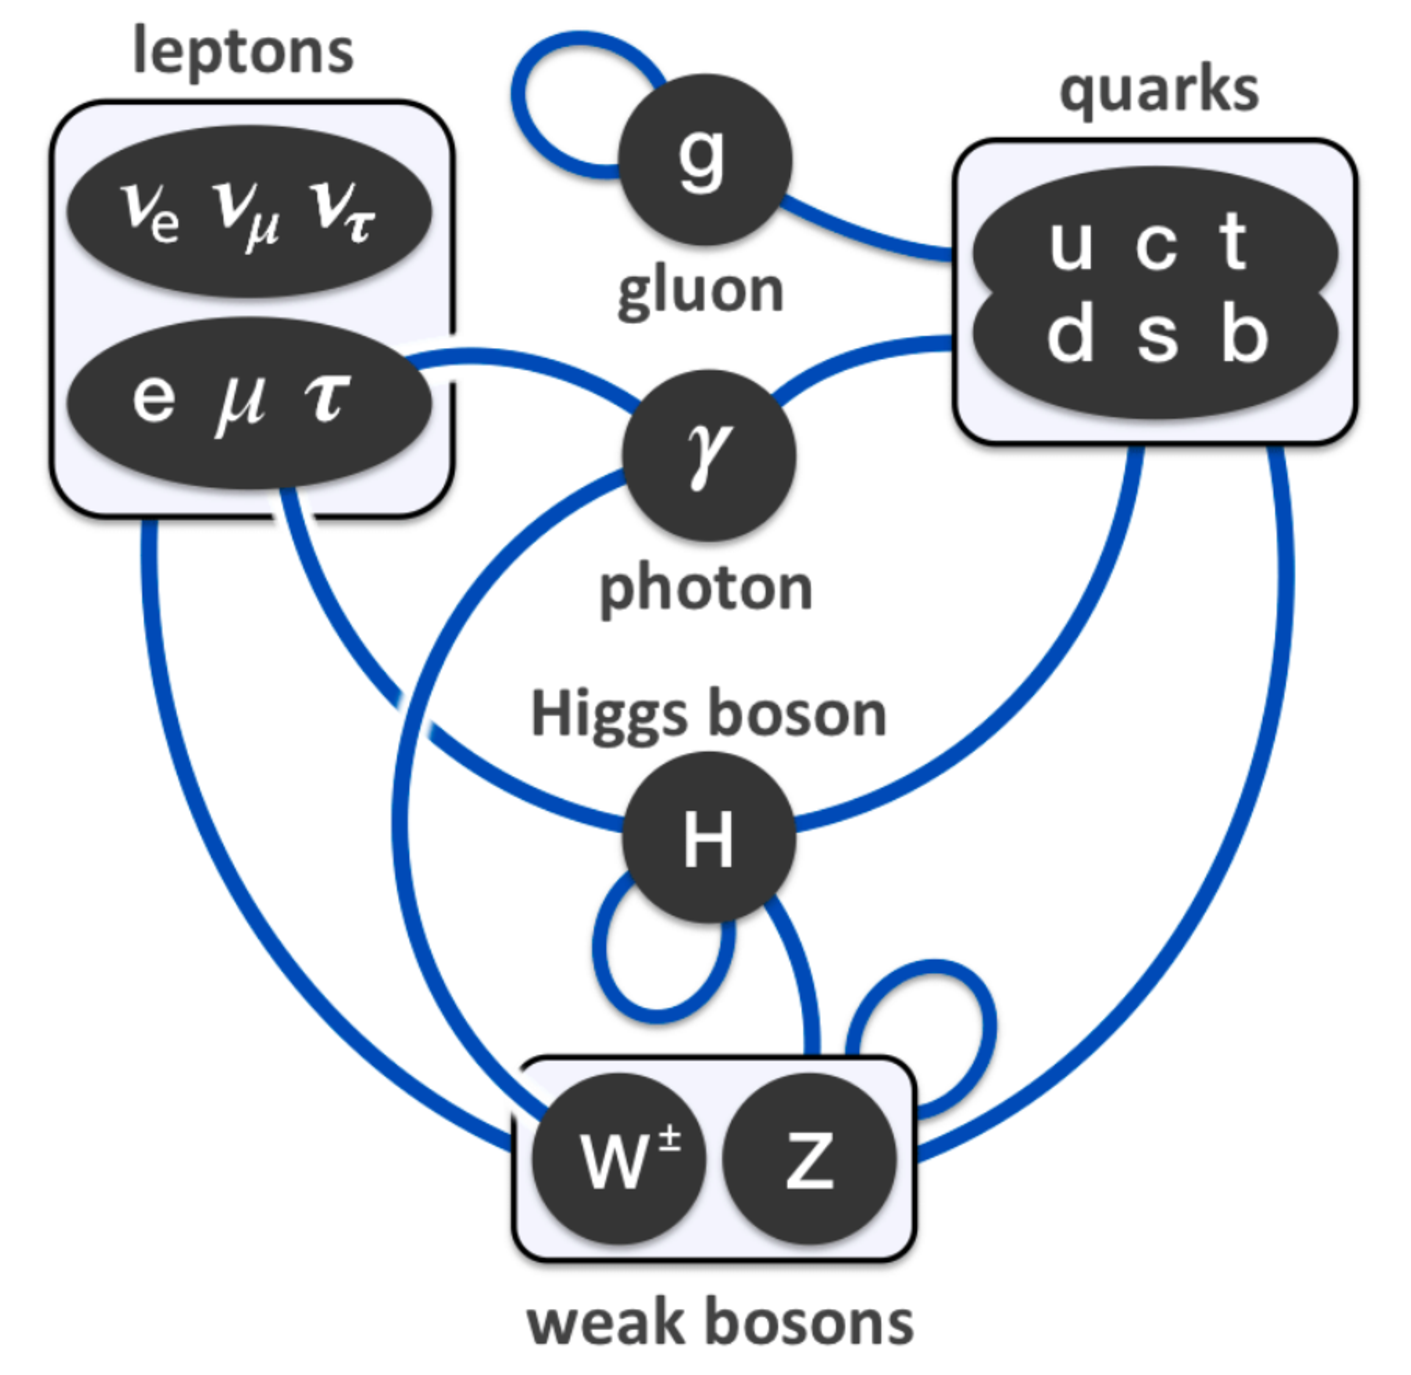
\includegraphics[width=0.5\linewidth]{figures/SMpic.pdf} 
   \caption[Overview of the Standard Model.]{The Standard Model with its fermions and bosons and the involved interactions. The solid blue line indicates which particles interact with each other. Loops depict self-interaction. \cite{SMpic}}
  \label{SMpic}                                     
 \end{center}
\end{figure}
%
Figure \ref{SMpic} summarizes the picture of the SM with its fermions and bosons. The lines indicate which particles interact with each other through the mediators, including self-interaction.
%Gedanken zum SM
%strong (n und p of same duplet) and weak isospin (chirality)
%%%%%%%%%%%%%%%%%%%%%%%%%%%%%%%%%%%%%%%%%%%%%%%%%%%%%%%%%%%%%%%%%%%%%%%%%%%%%%%%%%%%%%%%%%%%%%%%%%%%%%%%%%%%%%%%%%%%%%%%%%%%
\section{Beyond the scope of the Standard Model}\label{beyondSM}
Nevertheless, there are still many puzzles left which are not described by the SM. This circumstance keeps physicists well motivated to gain further progress and to push the frontiers of our understanding. \cite{Nair} In the following some of the issues are briefly described, like neutrino masses, quantum gravity, the hierarchy problem and supersymmetry.
\paragraph{Neutrino masses} are confirmed by various neutrino oscillation experiments \cite{Kajita}\cite{McDonald}, although the SM does not predict neutrino masses. The neutrino flavor states $\nu_\alpha$ with $\alpha=e,\mu,\tau$ are quantum entangled with the mass states $\nu_i$ where $i=1,2,3$ described by an unitary matrix $U_{\alpha i}$ \cite{mixing}. One possible extension of the SM, explaining neutrino masses, is the seesaw mechanism. Because of the absence of the right chirality spinor components $\Psi_{R,j}$, the mass term of the Dirac lagrangian $\bar{\Psi}_L\Psi_R+\bar{\Psi}_R\Psi_L$ cannot be formed in case of neutrinos. One possible solution is to describe the neutrino masses with a Majorana mass term, which introduces very massive right-chiral neutrinos\footnote{The large masses are consistent with the lack of evidence for right-chiral neutrinos at present day energies \cite{Nair}.} besides light weight left-chiral neutrinos. One caveat is that such right-chiral neutrinos as a consequence have to exist, although within the SM there are only left-handed neutrinos known. \cite{Nair}
\paragraph{Quantum gravity} could be the embedding of general relativity into a framework of quantum theory. Quantum theory provides a well confirmed framework for all theories describing particular interactions. Therefore it would be appealing to have a quantum formulation of gravity, following the example of all other fundamental forces and being one step closer to an unified description. From the point of view of cosmology, quantum gravity could be an encompassing theory for a more fundamental understanding where general relativity breaks down, when it comes to the initial conditions of the early universe or conditions of black holes. \cite{quantumgravity}
\paragraph{The hierarchy problem} is a current challenge in particle physics and arises from quadratic corrections to the weak scale. \cite{hierarchy} The hierarchy problem formulates the large differences of scales at which symmetries are broken. Considering a single, unifying symmetry, including the standard model symmetries $SU(3)_c\times SU(2)_L\times U(1)_Y$ (see chapter \ref{SM}), which has to be broken at scale $V$, because it is not manifested at the currently explored energy scales. A lower bound is $V\approx 10^{37}\,\text{GeV}$. At the same time spontaneous symmetry breaking takes place for $SU(2)_L\times U(1)_Y$ at scales of $v\approx\SI{246}{\giga\electronvolt}$\footnote{This is the vacuum expectation value for the Higgs field. \cite{VEV}} in order to allow for massive W$^\pm$ and Z$^0$ bosons as well es massive quarks and leptons. Within the framework of perturbation theory in quantum field theory such great scale differences are difficult to keep due to the fact that corrections of symmetry breaking are controlled by the highest masses involved. One approach for $v$ is $v^2=v_0^2\sum_{i=1}^kc_i\lambda^i V_0^2$ with the initial value $v_0$, the coupling constant $\lambda$ and general coefficients $c_i$. This shows that including the first order of correction, the equation becomes $v^2=v_0^2+c_1\lambda V_0^2$. The consequence is that $v_0^2$ has to be adjusted in such a way that it cancels out several decimal places, for instance 25, of the term $c_1\lambda V_0^2$, but the decimal places beyond that limit should add up to the scale of $\SI{246}{\giga\electronvolt}$. This fine tuning is an unsatisfactory situation, even worsened by adding more orders of quantum corrections. \cite{Nair} A non-perturbative solution to the hierarchy problem is proposed by supersymmetric models. \cite{nonperturbative} 
%passt hier wahrscheinlich doch nicht so gut hin, ist ja nicht so wesentlich jetzt für mich... Was ich mir vorstellen könnte ist, dass man das als relativierung zu GUT erklärt, dass auch GUT nicht die eierlegende Wollmilchsau ist--
\paragraph{Supersymmmetry (SUSY)} is a theory, which unifies fermions and bosons. The corresponding transformation can be described by an operator in spinor form $Q_{\alpha i}$ and converts fermion fields into boson fields and vice versa. Here $\alpha$ is the spinor index and $i$ are internal degrees of freedom. The field pairs are called superpartners (sparticles) and belong to the same multiplet. The difference between particles and sparticles is the spin quantum number which distinguishes them by half an unit of $\hbar$. \cite{Vergados} Due to the lack of evidence of sparticles in the same mass range as the already known elementary particles, also supersymmetry has to be broken. \cite{PhysTeV}. {\SUSY} is very attractive, because it can solve the hierarchy problem, achieve gauge unification and can even provide a candidate for dark matter. \cite{Nagashima} There are two main categories of supersymmetric models, namely $R$-parity conserving and $R$-parity violating models. $R$ is a discrete symmetry in the coupling of particles and their superpartners, defined as \cite{Vergados}:
\begin{align}
                        R=(-1)^{2S+3B+L}=                                       \begin{cases}
                                        +1 & \, \text{for ordinary particles} \\
                                        -1 & \, \text{for {\SUSY} particles}     \end{cases}
                                        \text{,}
\label{Rparity}
\end{align}
where $S$ is the spin, $B$ the baryon number and $L$ the lepton number. An exactly conserved $R$-parity will result in a stable lightest supersymmetric particle and the {\SUSY} particles will be produced in pairs. Whereas a $R$-parity violation will result in singly producable sparticles and all of them are intrinsically unstable. \cite{Kuze}
%%%%%%%%%%%%%%%%%%%%%%%%%%%%%%%%%%%%%%%%%%%%%%%%%%%%%%%%%%%%%%%%%%%%%%%%%%%%%%%%%%%%%%%%%%%%%%%%%%%%%%%%%%%%%%%%%%%%%%%%%%%%
\section{Leptoquarks}\label{LQmodels}
Different shortcomings of the standard model open up chances to extend the current understanding of elementary particle physics with concepts briefly introduced in chapter \ref{beyondSM}. One basic idea develops the symmetry approach further, taking the current symmetries as an example (see chapter \ref{SM}), into a grand unified theory ({\GUT}). This can be made possible by embedding the SM gauge groups $SU(3)_c\times SU(2)_L\times U(1)_Y$ into a higher symmetry $G_\text{{\GUT}}$. This group has to be broken at the so called ${\GUT}$-scale of $\sim 10^{16}\,\SI{}{\giga\electronvolt}$ to such an extent that the three SM interactions occur as separate interactions below this scale. \cite{PhysTeV} The previously mentioned issues in chapter \ref{beyondSM} already gave a clue on this unification concept in different degrees of manifestations and show that {\GUT} can be a solution for different issues, for example the gauge hierarchy problem \cite{hierarchyproblem}\cite{issuesGUT}, the generation problem \cite{issuesGUT}, the parameter problem \cite{issuesGUT} and neutrino masses \cite{neutrinoAndGUT}. {\GUT}s imply new gauge bosons called leptoquarks (LQ), which would explain the strong similarities between leptons and quarks. \cite{Nagashima}
%
%
\subsection{Leptoquarks and grand unified theories}\label{GUTandLQ}
The first {\GUT} model was proposed by Georgi and Glashow in 1974 \cite{GeorgiGlashow}. They proposed that the group $SU(5)$ incorporates all the fermions into one multiplet following the same universal coupling. This enables the possibility to transform leptons and quarks into each other with leptoquarks as mediators. Various global symmetries can embed the SM symmetries, but $SU(5)$ is the simplest one. \cite{Perkins} Although the Georgi-Glashow model had a great impact, this model has been ruled out \cite{GeorgiGlashowruledout}. It predicts a lifetime of the proton of $10^{30}\,\text{years}$, but the current experimental lower limit is $10^{33}\,\text{years}$\footnote{This value is vaild for the decay mode $p\rightarrow e^+K^0$. The predictions of the proton lifetime for other dominant decay modes -- relevant in {\GUT} models -- are higher and can be found in reference \cite{protonlifetime}.} \cite{Griffiths}\cite{protonlifetime}.\par%vllt noch einen Feynmangraph zum Proton Zerfall S. 408, Griffiths
Another unifying group would be $SO(10)$, which is broken to $SO(10)\rightarrow SU(4)_c\times SU(2)_L\times SU(2)_R$, where the leptons are treated as a forth color. \cite{PatiSalamExplanation} This model is known as Pati-Salam {\GUT} model \cite{PatiSalam}. Here also the right-handed leptons are included, acting differently than their left-chiral counterparts as it is expected for solutions of the neutrino masses for example. \cite{PatiSalamExplanation}\par
Other symmetry groups like $E_6$, inspired by superstring models, are also candidates for a {\GUT} theory. \cite{E6} $E_6$ has a rank of $6$ and is a member of the exceptional Lie groups. Furthermore it can be seen as the natural extension of $SU(5)$ and $SU(10)$ and naturally includes a greater set of particles. These additional particles can be, for instance, interpreted as dark matter candidates. \cite{E6explanation}
%
%
\subsection{Effective Leptoquark model}\label{effmodels}
%12 new mediators X (charge +-4/3, 3 colors = 6) und Y (charge +-1/3, 3 colors = 6) they couple to anti quarks and leptons (anti d liegt  im selben multiplet wie e-) griffiths
%X(Q,I3,Y)=(4/3,1/2,5/3), >(Q,I3,Y)=(1/3,-1/2,5/3) Nagashima
%gauge bosons both with su3 and su2 quantum numbers. these are associated with generators E_ar^+ a =1,2,3 r=4,5- These will be indicated as (X_mu)^alpha and (Y_mu)^alpha associated with r = 4,5 respectively. They occupy the positions indicated by alpha and r. the gauge bosons associated with E_alphar^- are the adjoined of the above and will be indicated as (X_mu)_alpha and (Y_mu)_alpha or equivalently as (Xbar_mu)^alpha and (Ybar_mu)^alpha. the gauge bosons X und Y are triplets under su3 and doublets under su2 and have hypercharge xxx and xxx (wie bei griffiths) vergados
%The known fermions split into three generations each containing 15 states. for example the first generation comprises u and d each in three colors and helicity states, the e- in two helicity states and the nu_e with one helicity state. by convention su5 multiplets are written down as LH states and  RH states are replaced by LH antiparticles (since CP symmetry e-_Land e+_L are equivalent, the RH states of course appear in seperate multiplets) Perkins
\begin{table}[htbp]
		\centering
                \renewcommand{\arraystretch}{1.2}       
		\begin{tabular*}{\linewidth}{@{\extracolsep{\fill}}cccc|cccc}
		\hline
		\hline
		\multicolumn{4}{c|}{$|F|=2$ leptoquarks}&  \multicolumn{4}{c}{$|F|=0$ leptoquarks}     
		\\
		\hline
		LQ       &       $Q/e$   & $T_3$   &       decay   &       LQ       &       $Q/e$   & $T_3$   &       decay   
		\\
		\hline
		$S_{0,L}$       &$-1/3$       &$0$     &$l^{-}_{L}u_L$ or $\nu_Ld_L$         &$V_{0,L}$      &$-2/3$     &$0$      &$l^{-}_{L}\bar{d}_R$ or $\nu_L\bar{u}_R$
		\\
                $S_{0,R}$       &             &        &$l^{-}_{R}u_R$                      &$V_{0,R}$      &            &         &$l^{-}_{R}\bar{d}_L$ 
                \\
                \hline
                $\tilde{S}_{0,R}$       &$-4/3$       &$0$     &$l^{-}_{R}d_R$              &$\tilde{V}_{0,L}$      &$-5/3$     &$0$      &$l^{-}_{R}\bar{u}_L$ 
                \\
                \hline
                $S_{1,L}$       &$-4/3$       &$-1$     &$l^{-}_{L}d_L$                     &$V_{1,L}$      &$-5/3$     &$-1$      &$l^{-}_{L}\bar{u}_R$
                \\
                         &$-1/3$       &$0$     &$l^{-}_{L}u_L$ or $\nu_Ld_L$              &              &$-2/3$     &$0$      &$l^{-}_{L}\bar{d}_R$ or $\nu_L\bar{u}_R$
                \\
                        &$2/3$       &$1$     &$\nu_Lu_L$                                &               &$1/3$     &$1$      &$\nu_L\bar{d}_R$
                \\
                \hline
                $V_{1/2,L}$       &$-4/3$       &$-1/2$     &$l^{-}_{L}d_R$                &$S_{1/2,L}$      &$-5/3$     &$-1/2$      &$l^{-}_{L}\bar{u}_L$
                \\
                $V_{1/2,R}$       &$-4/3$       &           &$l^{-}_{R}d_L$                &$S_{1/2,R}$      &$-5/3$    &             &$l^{-}_{R}\bar{u}_R$
                \\
                                &$-1/3$       &$1/2$      &$l^{-}_{R}u_L$                 &               &$-2/3$     &$1/2$      &$l^{-}_{R}\bar{d}_R$
                \\
                \hline
                $\tilde{V}_{1/2,L}$       &$-1/3$       &$-1/2$     &$l^{-}_{L}u_R$        &$\tilde{S}_{1/2,L}$      &$-2/3$     &$-1/2$      &$l^{-}_{L}\bar{d}_L$
                \\
                                &$2/3$       &$1/2$     &$\nu_Lu_R$                     &                &$1/3$     &$1/2$      &$\nu_L\bar{d}_L$
                \\
		\hline
		\hline
		\end{tabular*}
		\caption[Overview of the scalar and vector leptoquarks proposed by the minimal-Buchm\"{u}ller-R\"{u}ckl-Wyler model.]{Overview of the scalar (S) and vector (V) leptoquarks proposed by the minimal-Buchm\"{u}ller-R\"{u}ckl-Wyler model with their third component of the weak isospin $T_3$, electric charge $Q$ and fermion number $F$. The fourth column shows possible decay modes of the leptoquarks. \cite{Kuze}}
\label{LQstable}
\renewcommand{\arraystretch}{1}
\end{table}
%
All the {\GUT} models, which are briefly mentioned in section \ref{GUTandLQ}, share a common implication, namely the introduction of new gauge bosons called leptoquarks. This implication can be formulated as an effective theory of leptoquarks for energy scales below the {\GUT}-scale , describing the underlying physical concepts.\par     
The introduction of the effective leptoquark model closely follows \cite{Kuze}.\newline
Leptoquarks are color-triplet scalar $(S)$ or vector $(V)$ bosons having baryon and lepton numbers and carrying fractional electrical charge. \cite{Kuze} A general formulation of an effective Lagrangian for leptoquark interaction with SM fermions was proposed by Buchm\"{u}ller, R\"{u}ckl and Wyler \cite{BRW}. It assumes the following:
\begin{itemize}
\item[(i)] LQs have renormalizable interactions.
\item[(ii)] LQs have interactions invariant under the SM gauge symmetries $SU(3)_c\times SU(2)_L\times U(1)_Y$.
\item[(iii)] LQs couple only to the SM fermions, gauge bosons and the Higgs boson.
\item[(iv)] LQs are required to conserve the lepton number $L$ and the baryon number $B$ separately. They carry the fermion number
\begin{align}
                        F=3B+L
\label{fermionnumber}
\end{align}
with $|F|=0$ or $|F|=2$.
\item[(v)] Each LQ couples to only one quark-lepton generation, i.e. there are three LQ families.
\item[(vi)] LQs has pure chiral couplings to the SM fermions.
\end{itemize}
Condition (iv) makes sure that the proton instability is avoided. Condition (v) only allows inter-generational interactions and large tree-level flavor changing neutral currents and flavor universalities. Condition (vi) avoids direct contributions to chirally suppressed meson decays like $\pi\rightarrow e\nu$. The LQ model, fulfilling conditions (i)-(vi), is the so called minimal-Buchm\"{u}ller-R\"{u}ckl-Wyler effective model (mBRW) with the Yukawa coupling\footnote{Yukawa coupling describes the interaction of a scalar field with a scalar or pseudoscalar Dirac field \cite{Peskin}.} constant $\lambda$. \cite{Kuze}\newline
Fourteen different leptoquark types are proposed and are listed in table \ref{LQstable}. The same symbol represents LQs of different electric charge within an isospin family, i.e. $S_{1/2,L}$ stands for both, the $S_{1/2}$ state of charge $-\frac53$ and for $-\frac23$. Here $l_X$ are the left-handed lepton doublets in case of $X=L$ and the right handed lepton singlet in case of $X=R$. This differentiation between left-chirality and right-chirality is also valid for the quarks $q_X$ of up-type ($q=u$) or down-type ($q=d$). Seven of the fourteen LQs are scalars ($S_{0,L}$, $S_{0,R}$, $\tilde{S}_{0,R}$, $S_{1,L}$, $S_{1/2,L}$, $S_{1/2,R}$, $\tilde{S}_{1/2,L}$) and seven are vectors ($V_{0,L}$, $V_{0,R}$, $\tilde{V}_{0,R}$, $V_{1,L}$, $V_{1/2,L}$, $V_{1/2,R}$, $\tilde{V}_{1/2,L}$) with their fermion number $|F|=0$ and $|F|=2$. For specific models based on mBRW the branching ratio $\beta(LQ\rightarrow lq)$ is usually fixed to values like $0$, $\frac12$ or $1$. \cite{Kuze}\par
From the experimentalists' point of view it makes sense to expand the phenomenology of leptoquarks and ease some restrictions of the mBRW model, giving rise to more generic models. This means a broader sensitivity to possibly new physics in the face of already determined exclusion limits. One example is to consider the  branching ratio $\beta$ as a free parameter. Relaxing condition (iv) or (v) in the lepton sector could open new lepton-flavor violating decays. As a result the search for leptoquarks is more sensitive to various possibilities in the decay modes or to restrictions on the LQ-coupling. \cite{Kuze}
%https://edoc.ub.uni-muenchen.de/9100/1/Krobath_Gernot.pdf
%https://arxiv.org/pdf/hep-ph/9709356.pdf
%https://arxiv.org/pdf/hep-ex/0211048.pdf
%https://ac.els-cdn.com/037026938790637X/1-s2.0-037026938790637X-main.pdf?_tid=7fd73e94-a159-4098-a0c1-5df2ae6f102b&acdnat=1542542854_1685c5ae7ed0ff0824a75e01ecf264ea
%https://journals.aps.org/prd/pdf/10.1103/PhysRevD.8.1240
%https://journals.aps.org/prd/pdf/10.1103/PhysRevD.37.3165
%
%
\subsection{Leptoquark-like couplings in supersymmetry}
An additional generic picture can result from the point of view of supersymmetry. In $R$-parity violating {\SUSY} models squarks can produce leptoquark-like signature due to decay modes involving the Yukawa coupling. The left-chiral $\tilde{u}_L$\footnote{Usually the supersymmetric partner particles are denoted with a tilde $\left(\widetilde{\quad}\right)$.} squark couples to a $e^++d$ pair similar a leptoquark $\tilde{S}_{1/2,L}$ with an electric charge of $|Q|=\frac23 e$ would do. Accordingly the $\tilde{d}_R$ squark couples to a $e^-+u$ pair or $\nu_e+d$ pair and mimics a $S_0$ leptoquark of charge $|Q|=\frac13 e$. From an experimental point of view, the observation of such a decay is not only restricted to LQ models, but also has implications on constraints for the coupling of squarks in {\SUSY} models. \cite{Kuze}     
%
%
\subsection{Leptoquark pair production in proton-proton collisions}\label{LQpp}
For the search of leptoquarks, the mBRW model (see chapter \ref{effmodels}) is taken as a basis.\newline 
At proton-proton colliders, like the {\LHC}, leptoquarks can be be produced in pairs by gluon-fusion and smaller contributions of quark-fusion. These main processes are shown with feynman diagrams in figure \ref{LQpairs}. Figure \ref{gfa} and \ref{gfb} describes the gluon initiated production in the s-, t- and u-channel and figure \ref{qfc} the quark initiated production in the s- and t-channel. The last feynman diagram (lower right) is proportional to the square of the coupling constant ($\lambda^2$) due to the virtual lepton exchange \cite{hunter}\cite{Hewett}. Cross section calculations for such processes and further details can be found for example in reference \cite{Kramer}.  
%
\begin{figure}
  \centering
                \begin{subfigure}[t]{0.9\textwidth}
                \qquad\qquad
                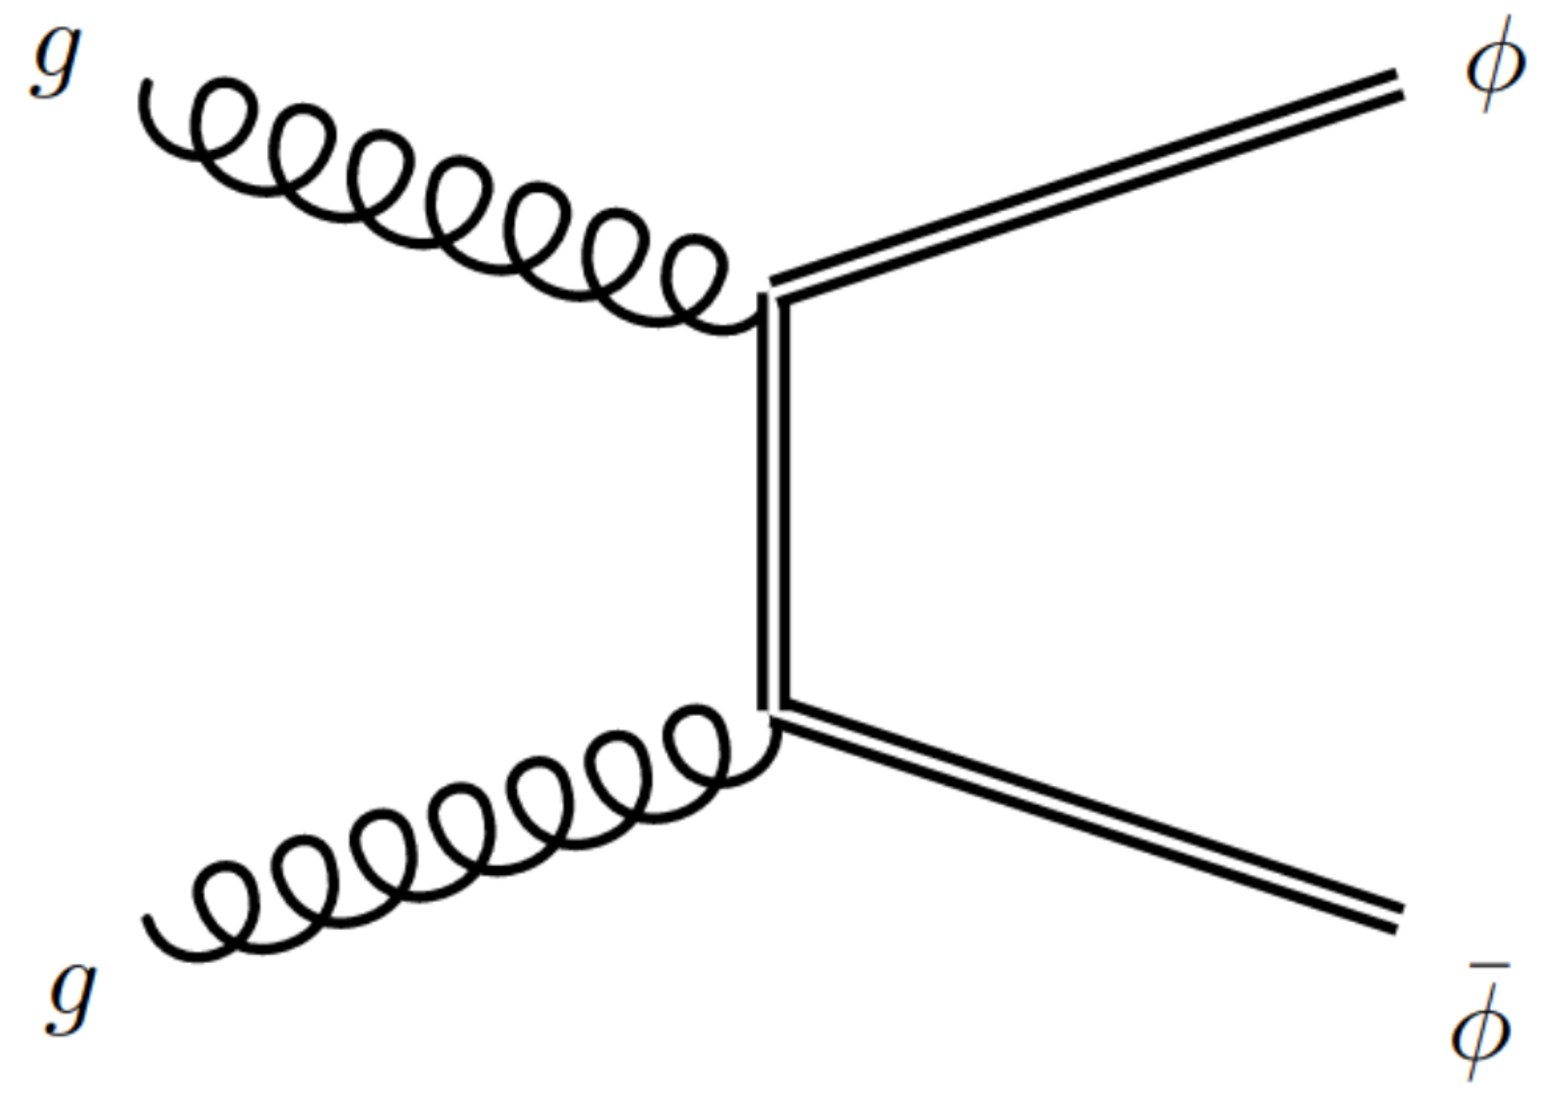
\includegraphics[width=0.4\textwidth]{figures/gfa.pdf}
                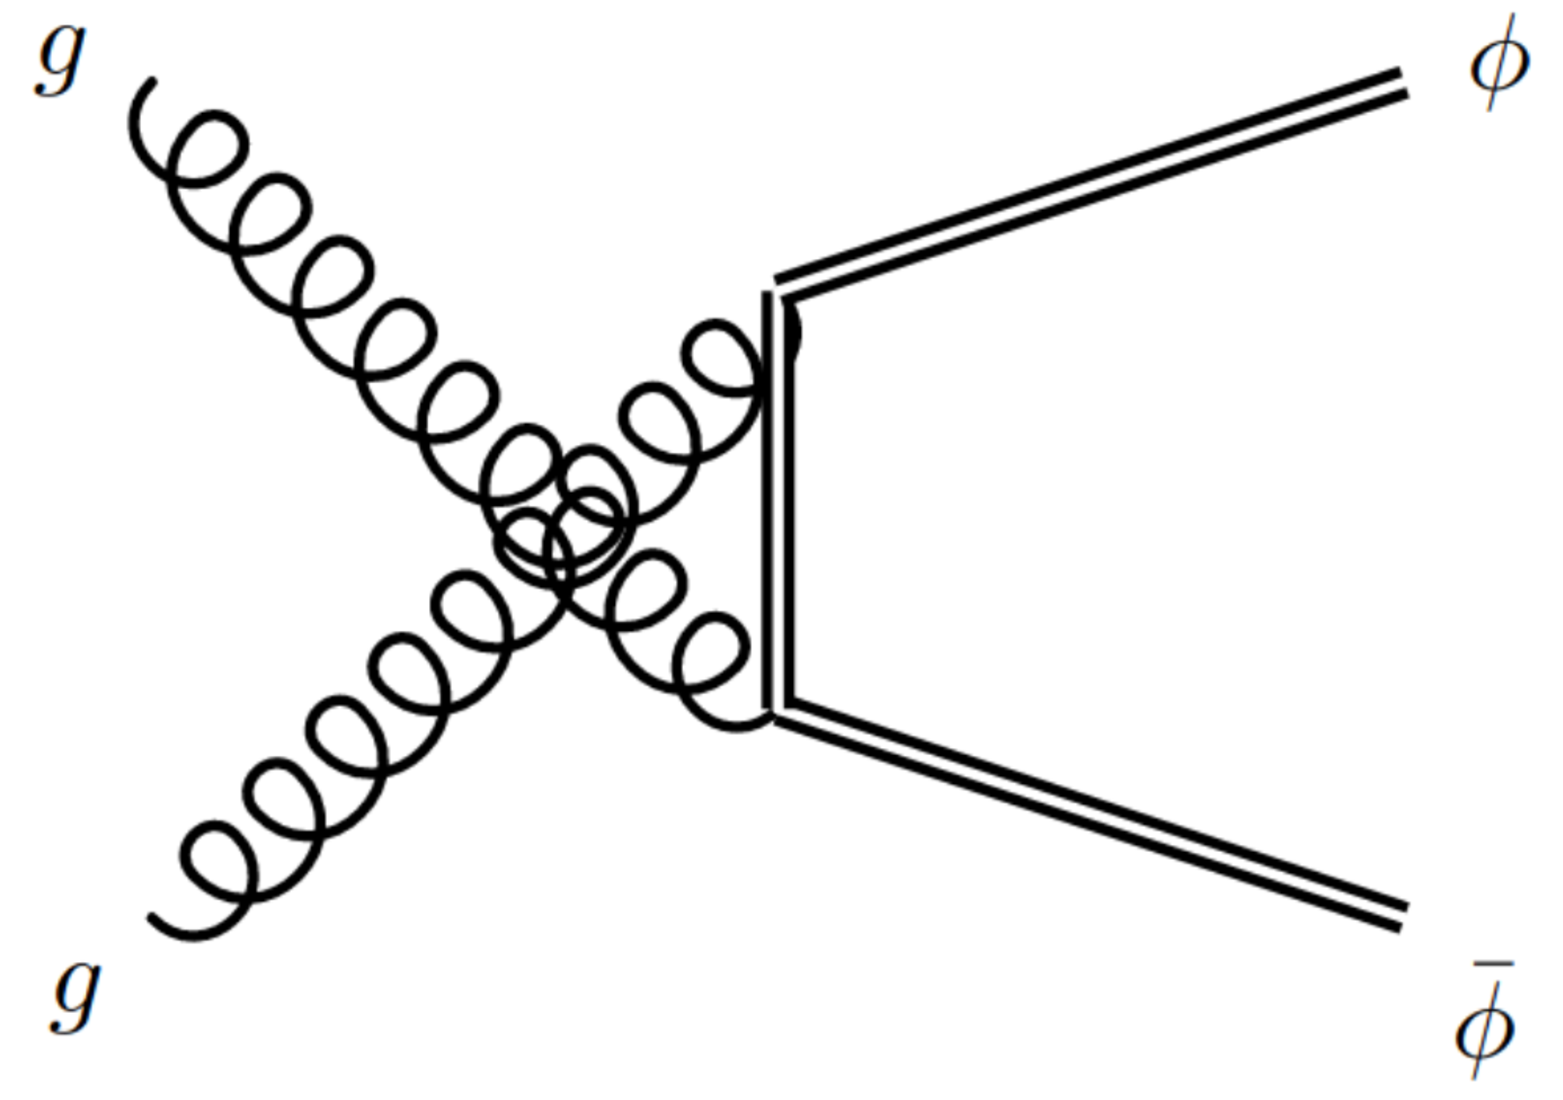
\includegraphics[width=0.4\textwidth]{figures/gfb.pdf}
                \subcaption{Leptoquark pair production via gluon-fusion in the t-channel and the u-channel.}
                \label{gfa}
                \end{subfigure}
                %
                \begin{subfigure}[t]{0.9\textwidth}
                \centering
                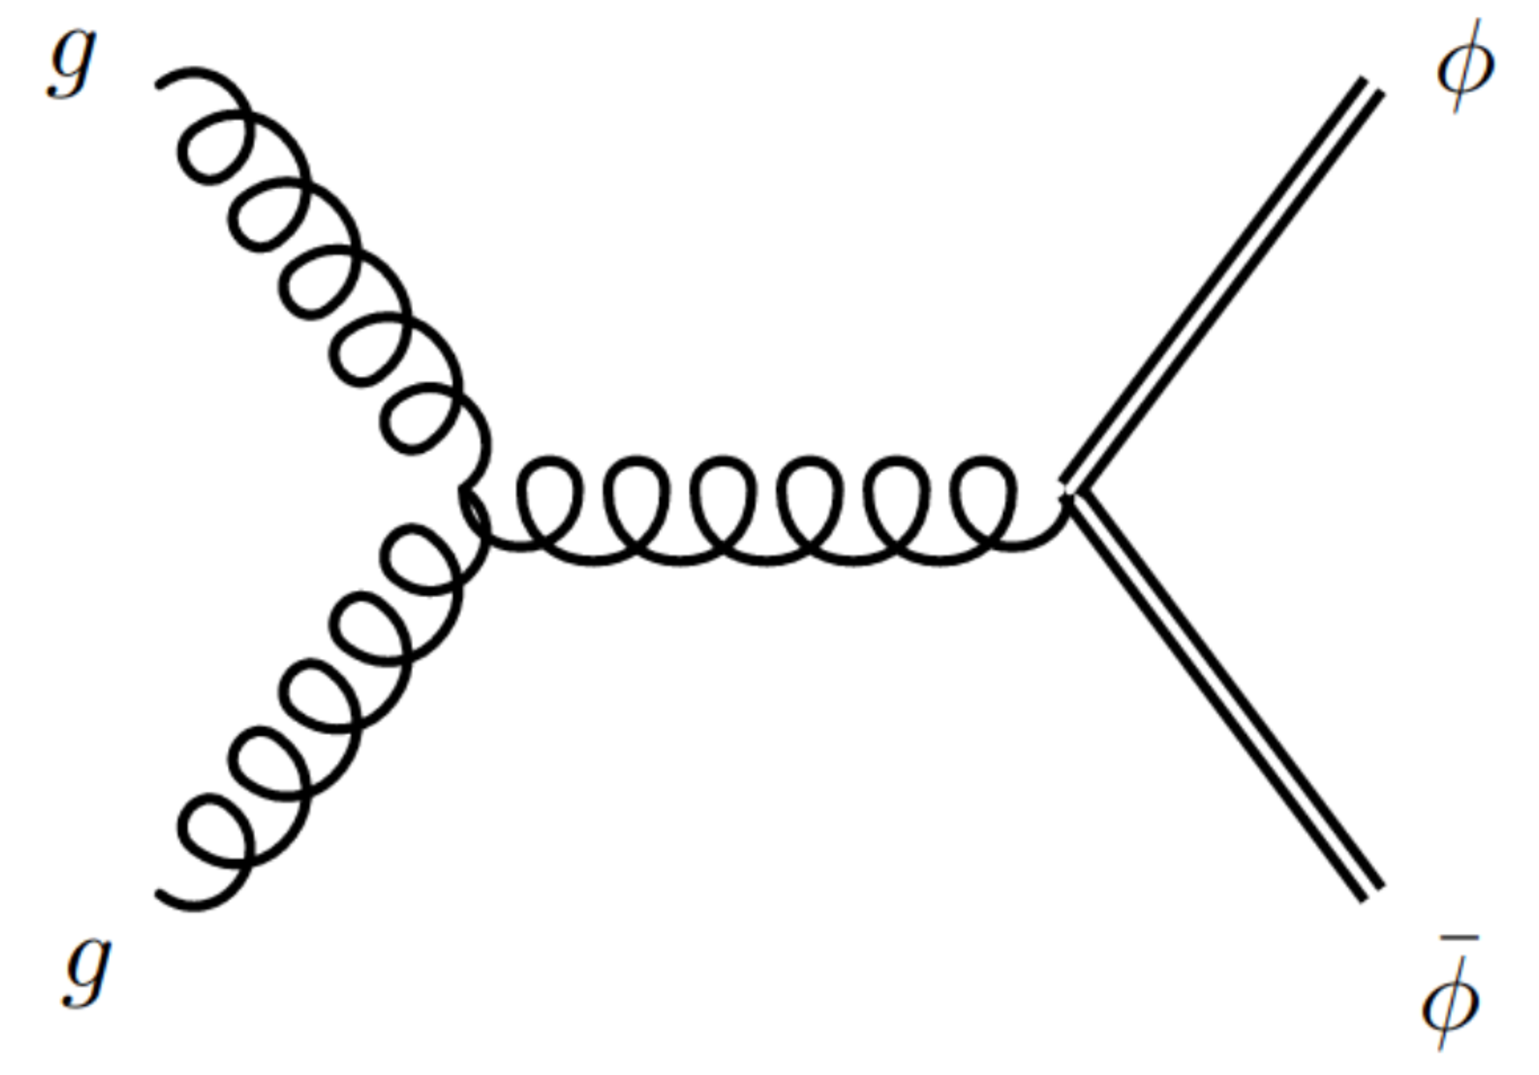
\includegraphics[width=0.4\textwidth]{figures/gfd.pdf}
                \subcaption{Leptoquark pair production via gluon-fusion in the s-channel.}
                \label{gfb}
                \end{subfigure}
                %
                \begin{subfigure}[t]{0.9\textwidth}
                \qquad\qquad
                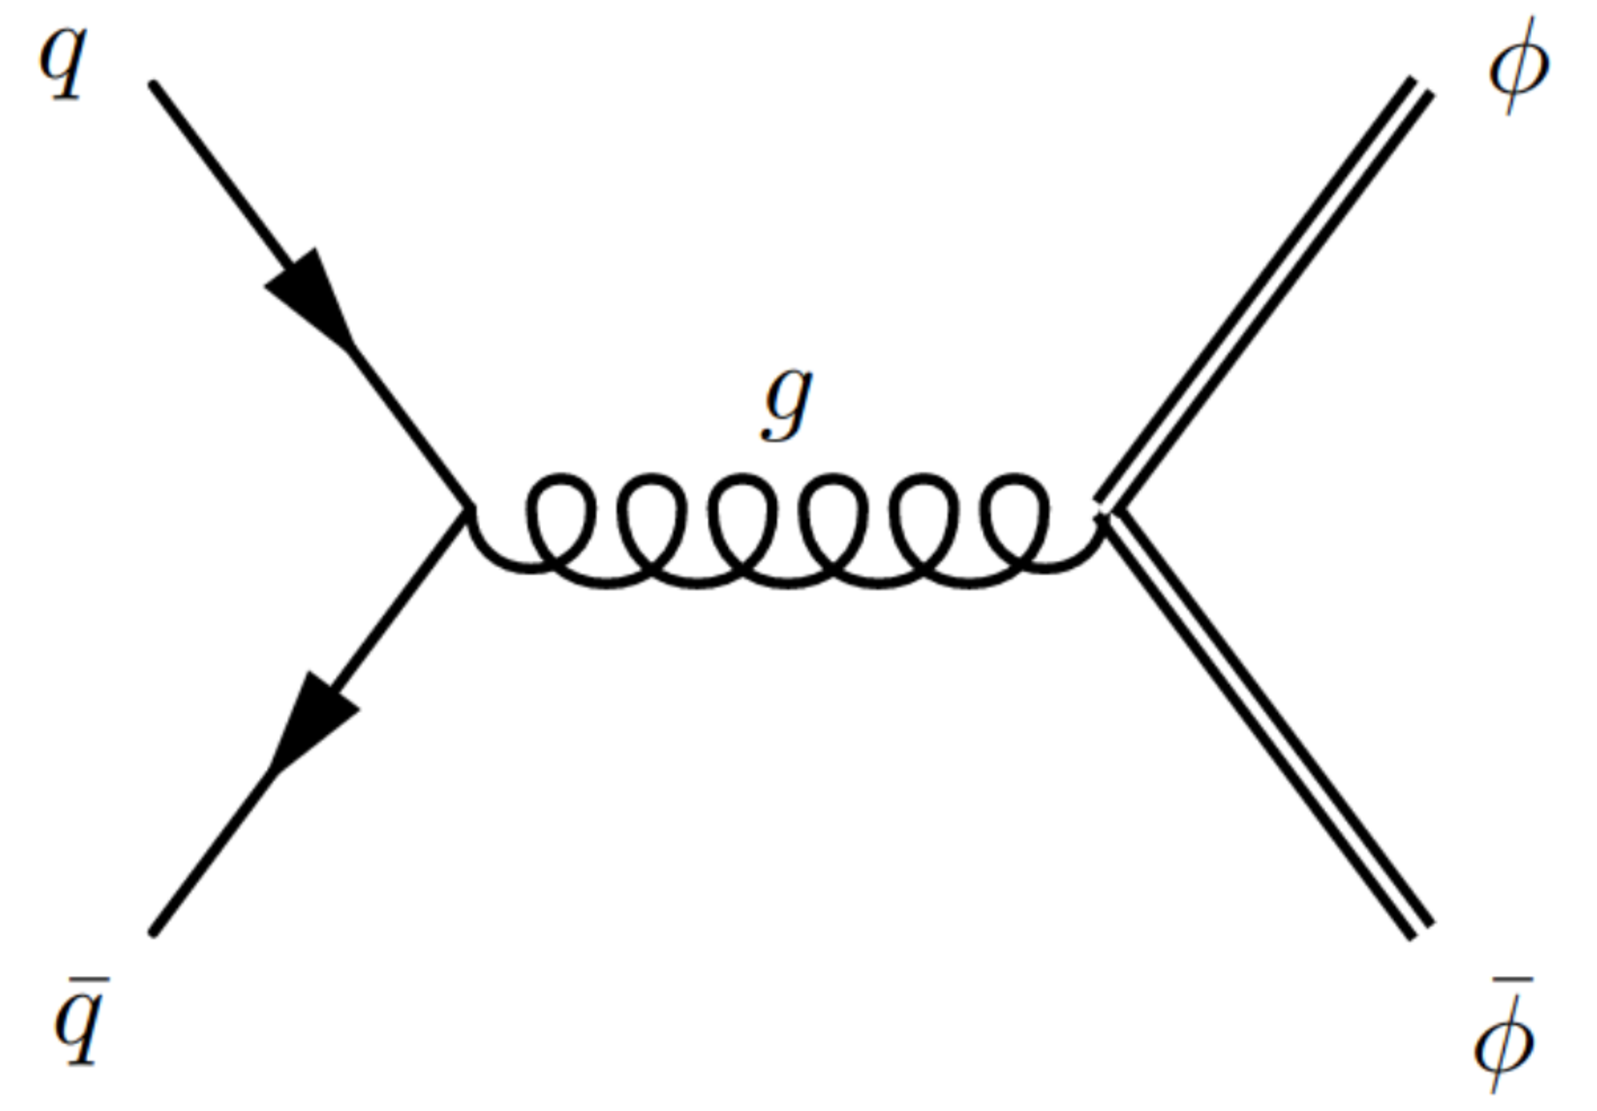
\includegraphics[width=0.4\textwidth]{figures/qfe.pdf}
                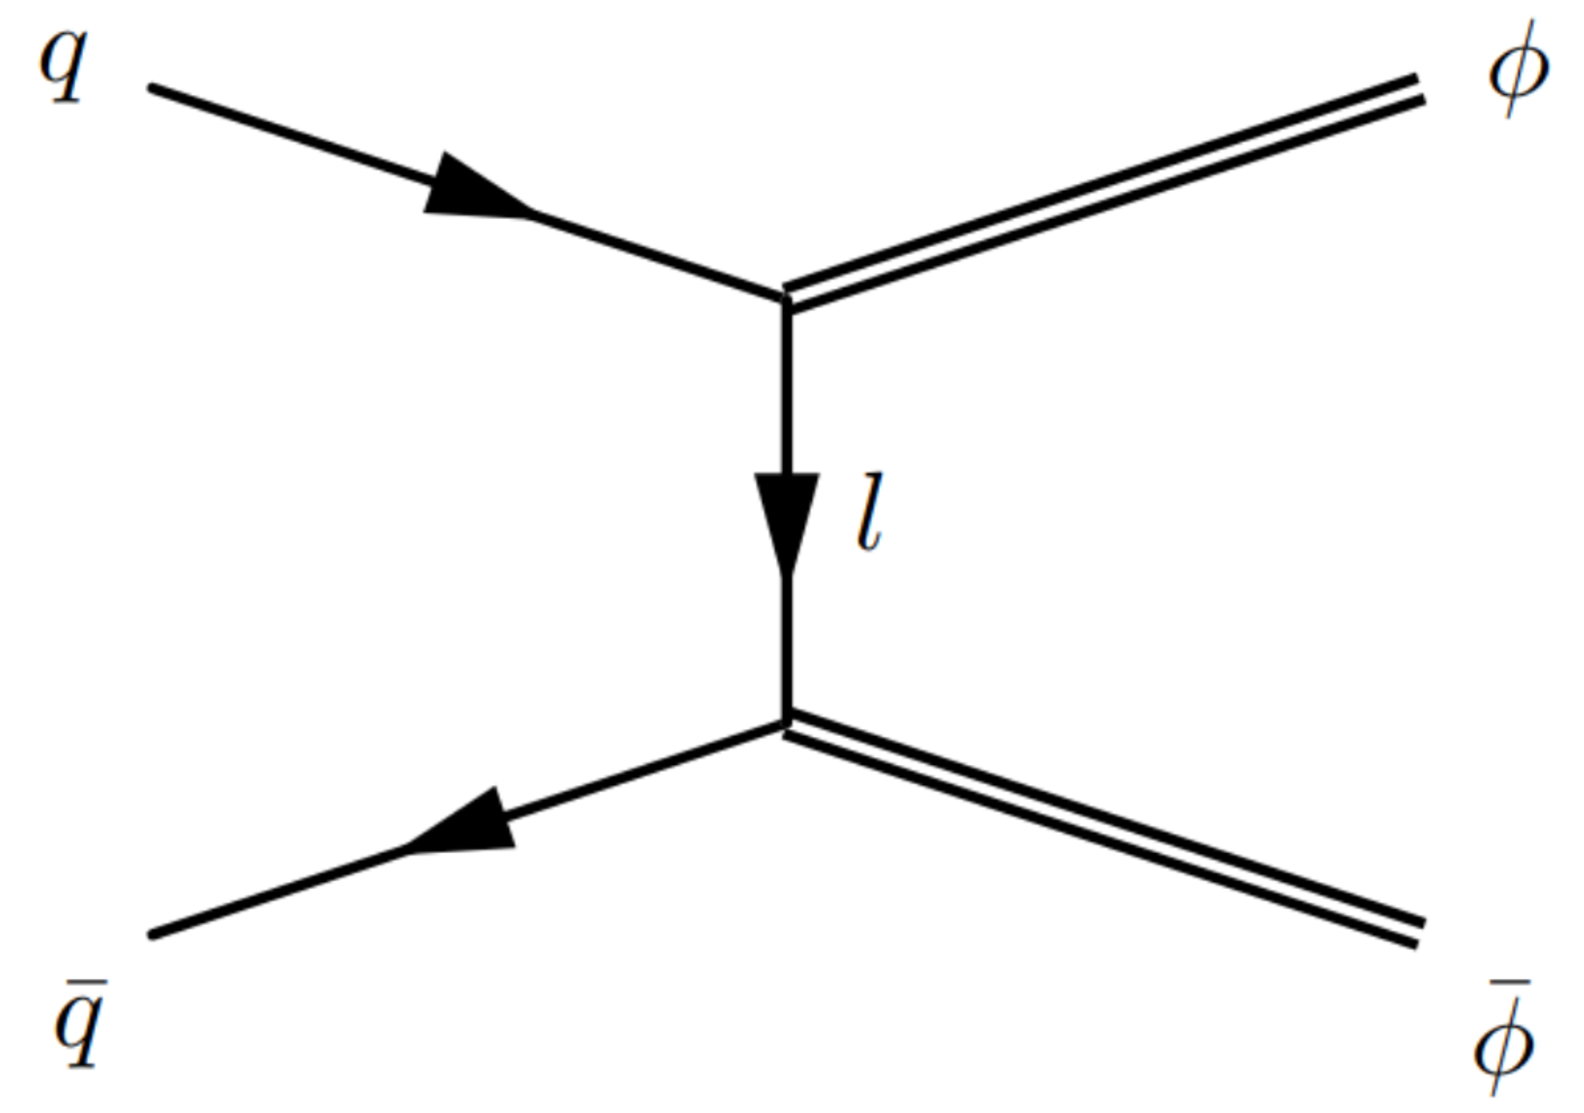
\includegraphics[width=0.4\textwidth]{figures/qff.pdf}
                \subcaption{Leptoquark pair production via quark-fusion in the s-channel and the t-channel.}
                \label{qfc}
                \end{subfigure}
                %
%
\caption[Feynman diagrams of leptoquark pair production processes at proton-proton colliders like the {\LHC}.]{Feynman diagrams of leptoquark pair production processes dominated by gluon-fusion (a), (b) and smaller contributions by quark-fusion (c) at proton-proton colliders like the {\LHC}. \cite{hunter}}
\label{LQpairs}
\end{figure}
%
%
%
%
%
The detectable final states are governed by the Yukawa coupling $\lambda_{lq}$ of the leptoquark directly to the quark $q$ and lepton $l$ (see figure \ref{YukawaLQ}). The model is defined by two parameters derived from $\lambda_{lq}$: The branching ratio $\beta$ and the coupling constant $\lambda$. They are connected to the Yukawa coupling constant by $\lambda_{lq}=\sqrt{\beta}\lambda$ for a charged lepton and by $\lambda_{lq}=\sqrt{1-\beta}\lambda$ for neutrinos. \cite{currentStatus:13TeVATLAS}\par
%
\begin{figure}[htbp]                                 
 \begin{center}                                       
  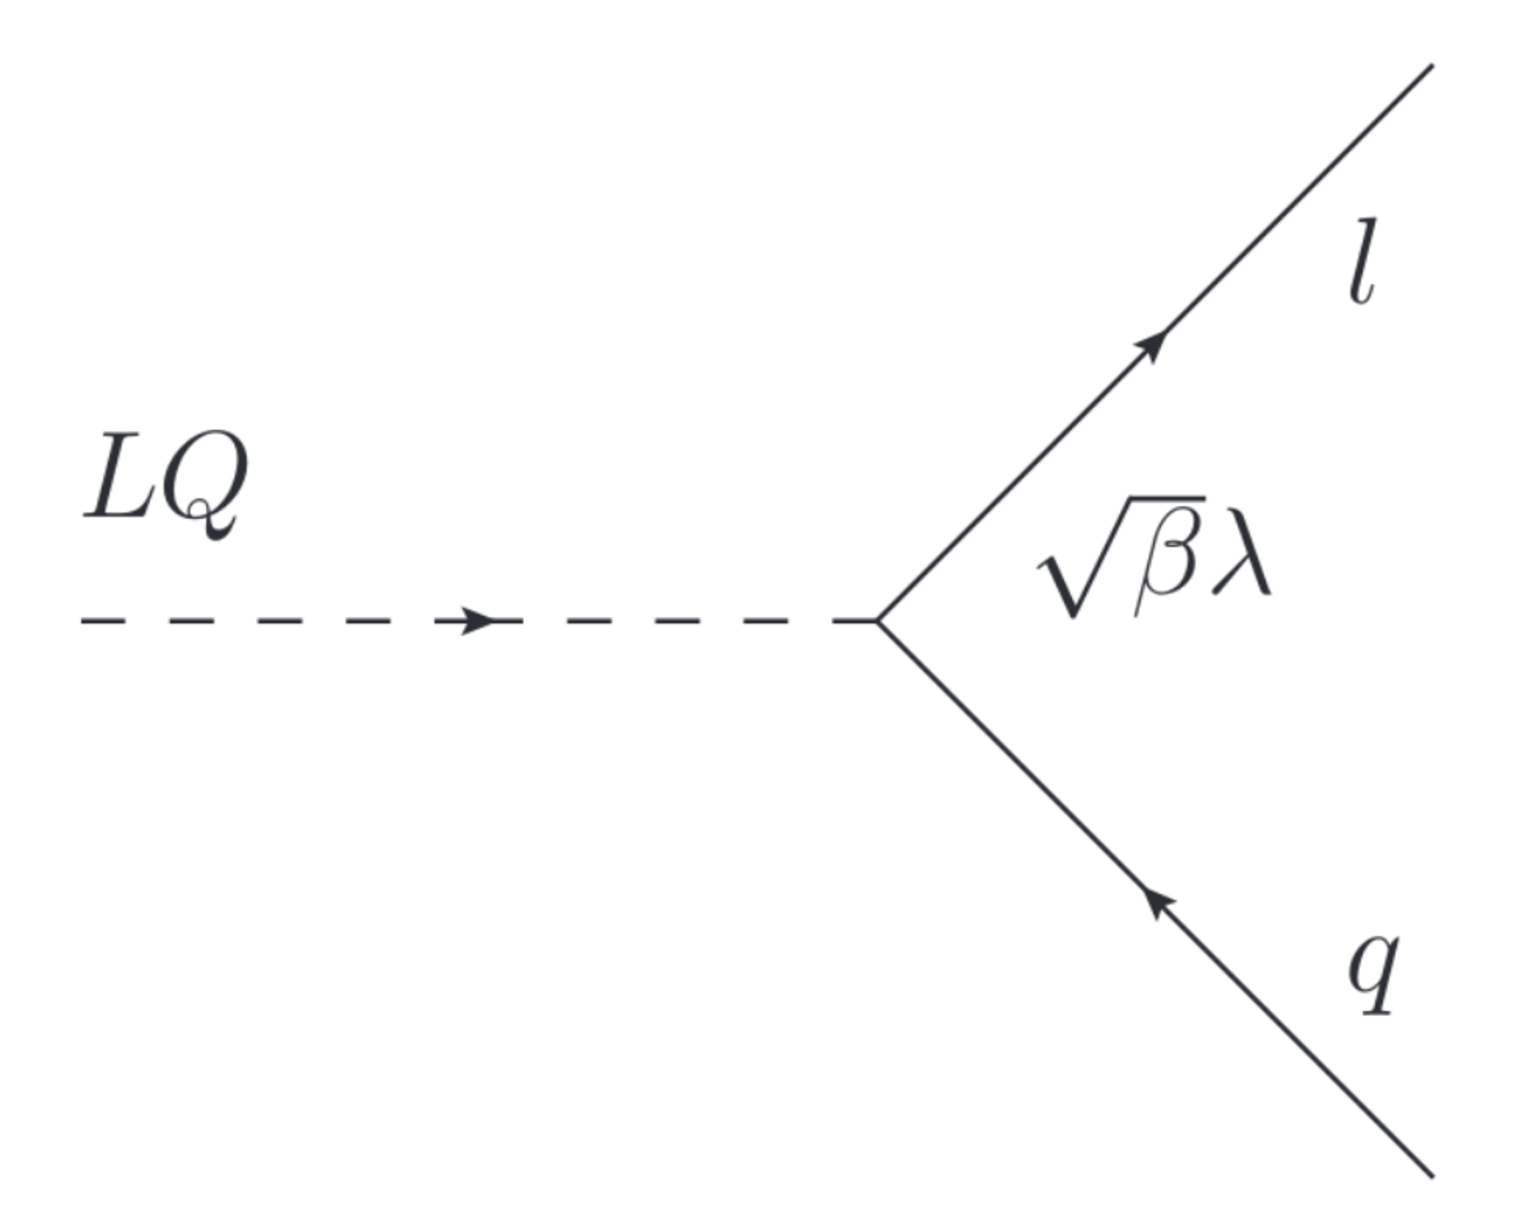
\includegraphics[width=0.4\linewidth]{figures/yukawa.pdf} 
   \caption[Feynman diagram of a leptoquark decay governed by Yukawa coupling.]{Feynman diagrams of a leptoquark decay into a lepton $l$ and a quark $q$ governed by Yukawa coupling $\lambda_{lq}=\sqrt{\beta}\lambda$. \cite{currentStatus:13TeVATLAS}}
  \label{YukawaLQ}                                     
 \end{center}
\end{figure}
%
The focus of this thesis lies on the search of pair produced scalar leptoquarks with the final state $LQ+LQ\rightarrow t\tau^{-}+\bar{t}\tau^{+}$. These final states would correspond to leptoquarks $S_{0,L}$ and $S_{1,L}$ (cf. table \ref{LQstable}). 
%Futher information on the search of vector leptoquarks can be found for example in \cite{vectorLQ} and \cite{vectorLQQ}. 
%https://cds.cern.ch/record/2308307/files/SUgS-18-001-pas.pdf guter Ausgangspunkt auch für LQ Literatur Suche
%
% eigentlich war geplant, dass die folgenden zwei Kapitel zu Kapitel data anaalysis gehören, allerdings findet Mahsana, dass das jetzt gleich kommen sollte
%
%
\subsection{Current status in the search for scalar leptoquarks}\label{currentStatus}
%Literatur dazu: current:<> in der .bib
Leptoquarks are a promising research field for physics beyond the SM. Various efforts are made with the physics program available at today's particle accelerators to search for LQ-like signatures. The following summarizes briefly the current status for the search for scalar leptoquarks at the {\LHC}.\par
LQ considered by the minimal-Buchm\"{u}ller-R\"{u}ckl-Wyler model (cf. section \ref{effmodels}) can result in various final states, which can be potentially detected by the {\ATLAS} or {\CMS} detector.\newline
The data samples recorded by the {\ATLAS} experiment in 2012 at a center of mass energy of $\sqrt{s}=\SI{8}{\tera\electronvolt}$ were searched for signal events of pair-produced LQs decaying to $LQ+LQ\rightarrow e^+q+e^-\bar{q}$, $LQ+LQ\rightarrow \mu^+q+\mu^-\bar{q}$, $LQ+LQ\rightarrow t\nu_\tau+q+\bar{t}\bar{\nu}_\tau$ and $LQ+LQ\rightarrow b\nu_\tau+q+\bar{b}\bar{\nu}_\tau$ at an integrated luminosity of $\SI{20.3}{\per\femto\barn}$. The search for first and second generation LQs was performed in the $e^+qe^-\bar{q}$ and $\mu^+q\mu^-\bar{q}$ channel. The integrated luminosity for the search of third generation LQs ($t\nu_\tau\bar{t}\bar{\nu}_\tau$ and $b\nu_\tau\bar{b}\bar{\nu}_\tau$) is $\SI{20.1}{\per\femto\barn}$. \cite{currentStatus:8TeVATLAS}\footnote{The search for scalar leptoquarks at $\sqrt{s}=\SI{7}{\tera\electronvolt}$ at the {\ATLAS} experiment is addressed by reference \cite{currentStatus:7TeVATLAS}.} For a branching ratio of the LQs of $\beta=1.0$ exclusion limits were found for the first and second generation LQs. The exclusion limit for first generation LQ masses are $m_{LQ1}<\SI{1050}{\giga\electronvolt}$ and for second generation LQ masses are $m_{LQ2}<\SI{1000}{\giga\electronvolt}$ at a confidence limit (CL) of $\SI{95}{\percent}$. For the third generation the mass exclusion limit at CL $\SI{95}{\percent}$ is $m_{LQ3}<\SI{625}{\giga\electronvolt}$ based on the $b\nu_\tau\bar{b}\bar{\nu}_\tau$ decay mode and $\SI{210}{\giga\electronvolt}<m_{LQ3}<\SI{640}{\giga\electronvolt}$ based on the $t\nu_\tau\bar{t}\bar{\nu}_\tau$ decay mode. \cite{currentStatus:8TeVATLAS}\par
A more recent study by the {\ATLAS} collaboration at $\sqrt{s}=\SI{13}{\tera\electronvolt}$ was published in reference \cite{currentStatus:13TeVATLAS} for first and second generation leptoquarks. The observed exclusion limits for the LQ mass at $\SI{95}{\percent}$ CL are $\SI{1100}{\giga\electronvolt}$ and $\SI{1050}{\giga\electronvolt}$ assuming a branching ratio of $\beta=1.0$. The study has increased the sensitivity for the leptoquarks and agrees with the former study \cite{currentStatus:8TeVATLAS}. The exclusion limits are extended \cite{currentStatus:13TeVATLAS} compared to the previous study.\par
The {\CMS} collaboration published a study for the search of third generation scalar leptoquarks decaying to a top quark and $\tau$-lepton at a center of mass energy of $\SI{13}{\tera\electronvolt}$.
%
\begin{figure}[htbp]                                 
 \begin{center}                                       
  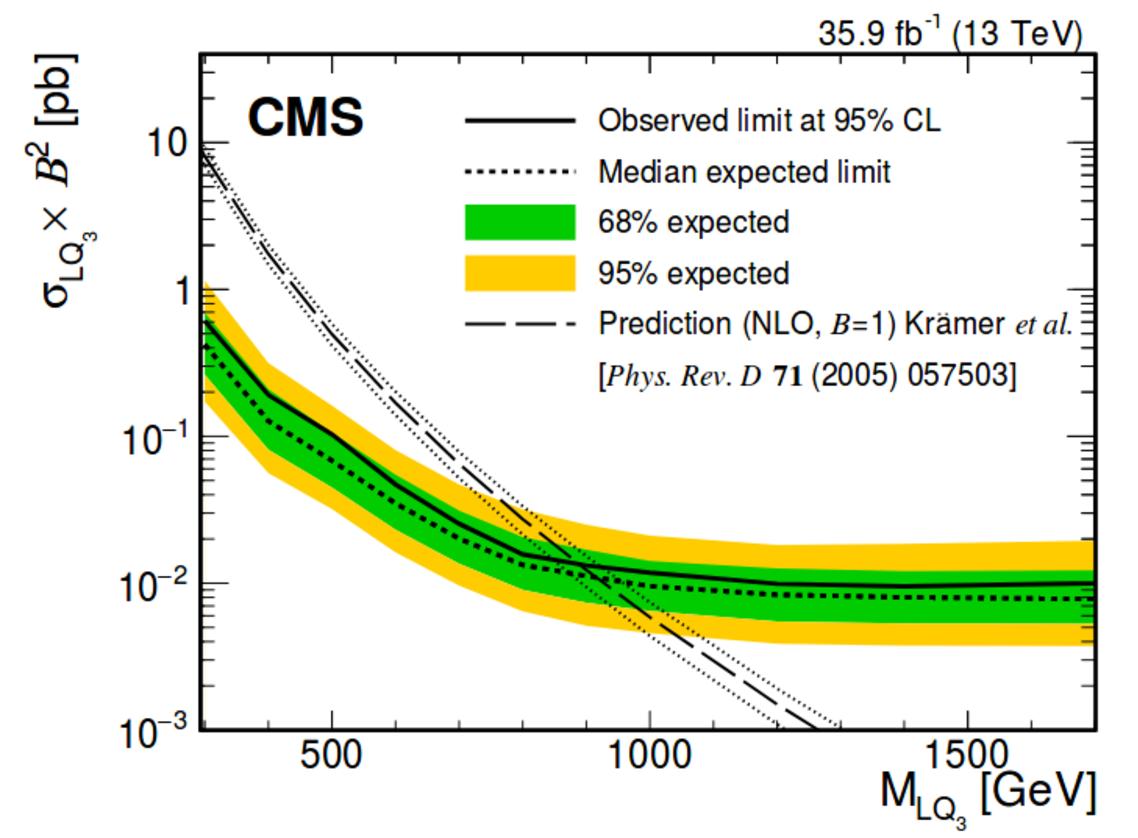
\includegraphics[width=0.6\linewidth]{figures/exclusionLQ.pdf} 
   \caption[Upper limits of the product of the cross section and $\beta^2$ depending on the leptoquark mass for the $t\tau^-\bar{t}\tau^+$ channel.]{Upper limits at CL $\SI{95}{\percent}$ of the product of the cross section and $\beta^2$ depending on the leptoquark mass for the $t\tau^-\bar{t}\tau^+$ channel (third generation) at $\sqrt{s}=\SI{13}{\tera\electronvolt}$ \cite{currentStatus:13TeVATLAS}.}
  \label{exclusionLQ}                                     
 \end{center}
\end{figure}
%
The corresponding integrated luminosity is $\SI{35.9}{\per\femto\barn}$. The results agree with the standard model expectation and no evidence for LQ pair production was found. The study excludes LQ with masses below $\SI{900}{\giga\electronvolt}$ at a branching fraction of $\beta=1.0$ and at a CL of $\SI{95}{\percent}$. Figure \ref{exclusionLQ} shows upper limits at CL $\SI{95}{\percent}$ of the product of the cross section and $\beta^2$ depending on the leptoquark mass for the $t\tau^-\bar{t}\tau^+$ channel. These results are the most stringent limits to date for the production of third generation LQs decaying to top quark and $\tau$-lepton. \cite{currentStatus:13TeVCMS}\par
%%%%%%%%%%%%%%%%%%%%%%%%%%%%%%%%%%%%%%%%%%%%%%%%%%%%%%%%%%%%%%%%%%%%%%%%%%%%%%%%%%%%%%%%%%%%%%%%%%%%%%%%%%%%%%%%%
\subsection{Starting point and research question for the analysis}\label{startingpoint}
This work is enclosed in the general research context briefly described in section \ref{currentStatus} and makes a contribution to the search of pair-produced scalar LQs of type $S_{0,L}$ and $S_{1,L}$ (cf. table \ref{LQstable}) decaying to $LQ+LQ\rightarrow t\tau^{-}+\bar{t}\tau^{+}$ at the {\ATLAS} experiment. The common difficulty in searches for exotic particles is that in the measured datasets signal and background contributions appear as one entity. To reliably distinguish between signal and background events it would be ideally to break the data down into its single constituents. Of course this is not possible, but using Monte Carlo simulations provides up a chance for a better understanding of signal and background contributions in real data (see also section \ref{MCsim}). Although this work does not presents a full search strategy for third generation leptoquarks it provides insight into $\tau$ reconstruction efficiencies and background studies for the search of LQ-signal signatures based on Monte Carlo samples (see section \ref{signalANDbgEff}). Within the context of the $t\tau^{-}+\bar{t}\tau^{+}$ channel, efficiencies reflect the ability to successfully reconstruct a tau lepton in the detector. The thesis makes further contributions to fake rate estimations for objects that incorrectly mimic the signature of a tau lepton. It also presents kinematic variables (see section \ref{Kinematics}) within the event selection (see section \ref{eventselection}) that are sensitive to the decay of third generation leptoqurk pairs. By taking into account findings from the kinematic distributions, the efficiency and fake rate contributions, the discovery significances based on signal samples are calculated, which allows first optimization steps (see section \ref{significance}). The used data sets are from the data taking periods $2015$, $2016$, $2017$ and partly $2018$ adding up to an integrated luminosity of $\SI{140}{\per\femto\barn}$.\par   
The search for third generation LQ decaying to top quarks and $\tau$-leptons is complex because of the multiple objects resulting from the subsequent decays of the heaviest quark and heaviest lepton. 
%
%
\begin{figure}
 \centering
  \begin{subfigure}[t]{0.45\textwidth}
   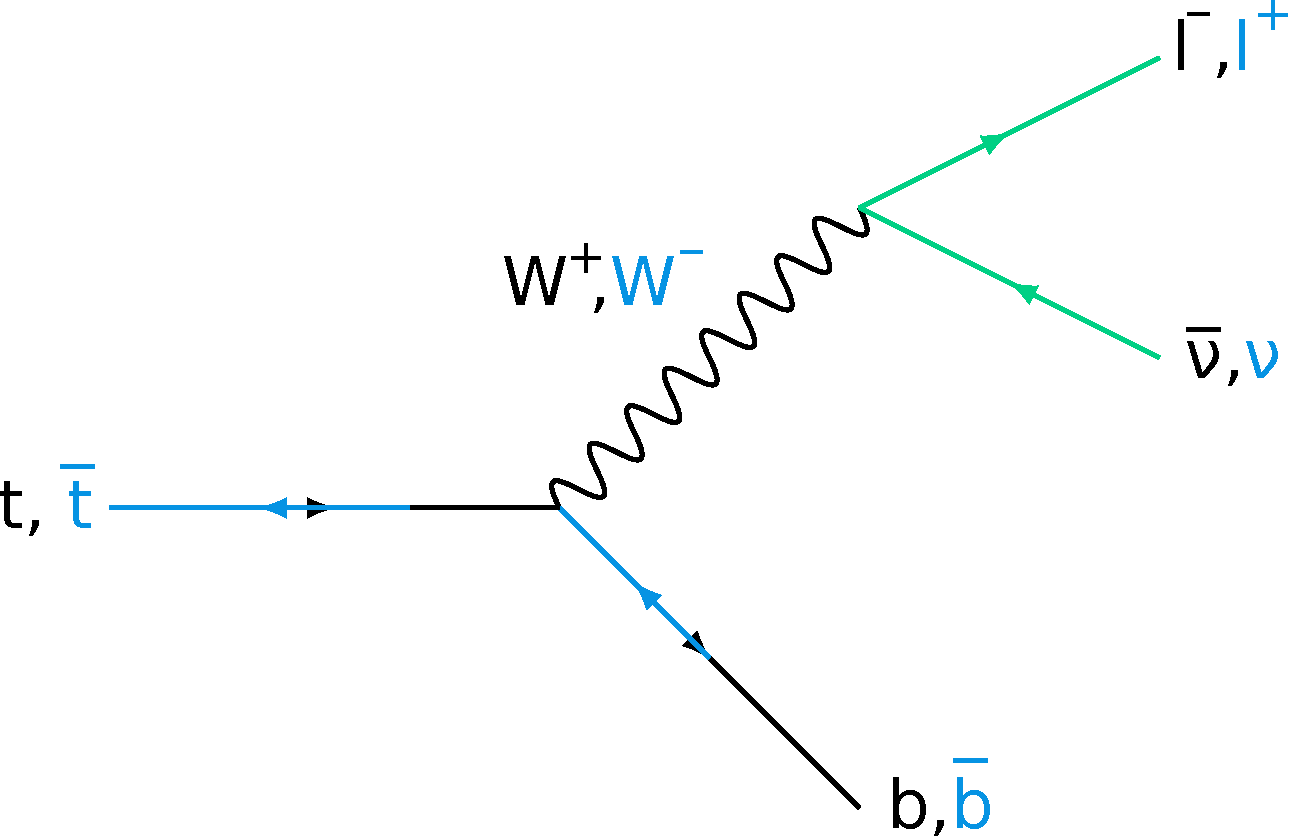
\includegraphics[width=\textwidth]{figures/t_leptonic.pdf}
    \subcaption[Leptonic top decay.]{Leptonic single-top decay. Black depicts the top decay, whereas blue depicts the anti-top decay. Leptons of different flavors are depicted as $l$ with the corresponding neutrino flavor $\nu_l$.}
   \label{topleptonic}
  \end{subfigure}
  \quad
  \begin{subfigure}[t]{0.45\textwidth}
   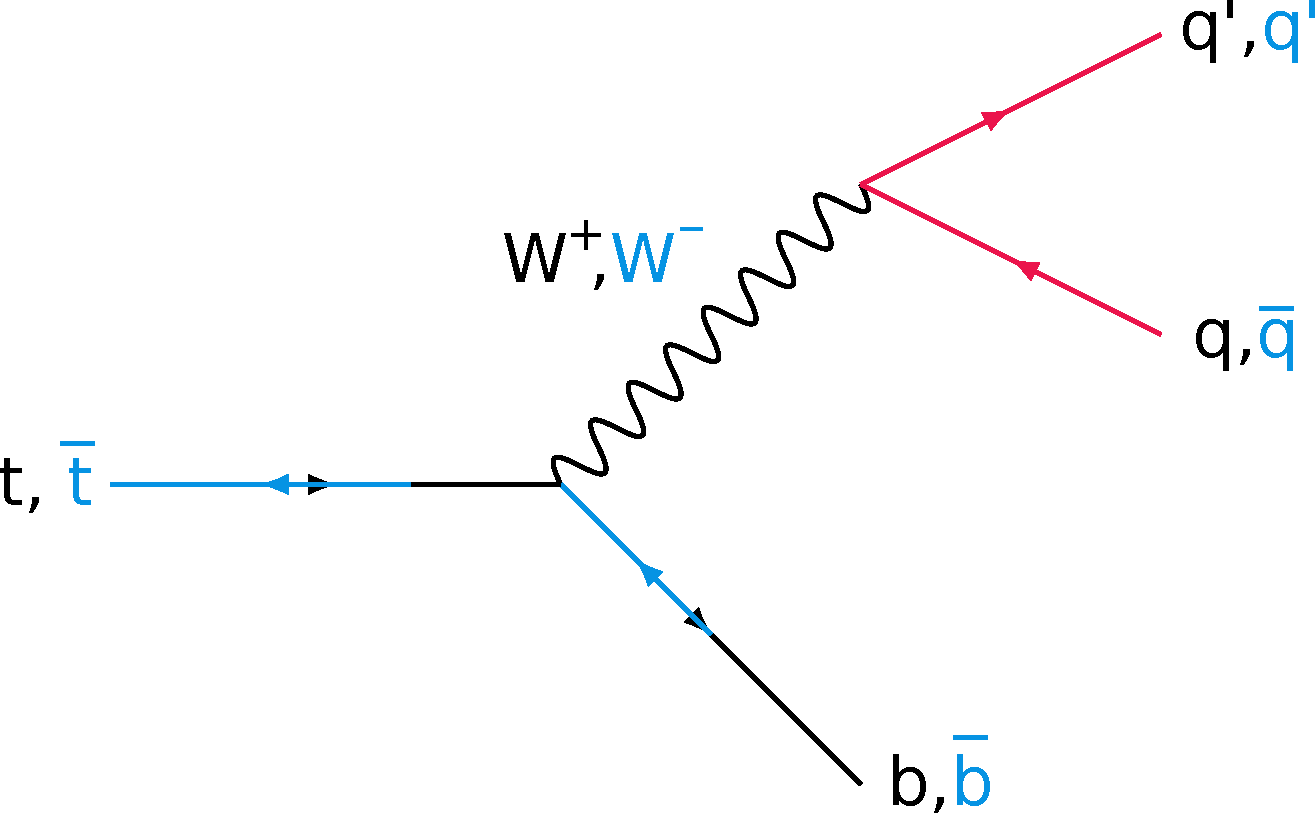
\includegraphics[width=\textwidth]{figures/t_hadronic.pdf}
   \subcaption[Hadronic top decay.]{Hadronic single-top decay. Black depicts the top decay, whereas blue depicts the anti-top decay.}
   \label{tophadronic}
  \end{subfigure}
 \caption[Leptonic and hadronic top decay.]{Leptonic (a) and hadronic (b) single-top decay.}
 \label{topdecay}
\end{figure}
%
The top quark decays weakly into $t\rightarrow Wq$ with $q=b,s,d$. The main decay mode involves the bottom quark. The subsequent decay of the weak gauge boson $W$ is either hadronically ($\SI{66.5\pm 1.4}{\percent}$) or leptonically ($\SI{34\pm1.0}{\percent}$) \cite{PhysRevD}. This is shown in figure \ref{topdecay}, where the black diagram paths indicates the top decay and the blue diagram path indicates the the anti-top decay. Leptons of different flavors are depicted as $l$ with their corresponding neutrinos $\nu_l$. This means that top-pairs can produce fully-leptonic decays following both the feynman diagram of figure \ref{topleptonic}, fully-hadronic decays following both the feynman diagram of figure \ref{tophadronic} and semi-leptonic decays, where one top decays leptonically and one hadronically. The overall percentage of the final state evolving from top pair pairs is shown in figure \ref{topcake}.\newline
%
\begin{figure}[htbp]                                 
 \begin{center}                                       
  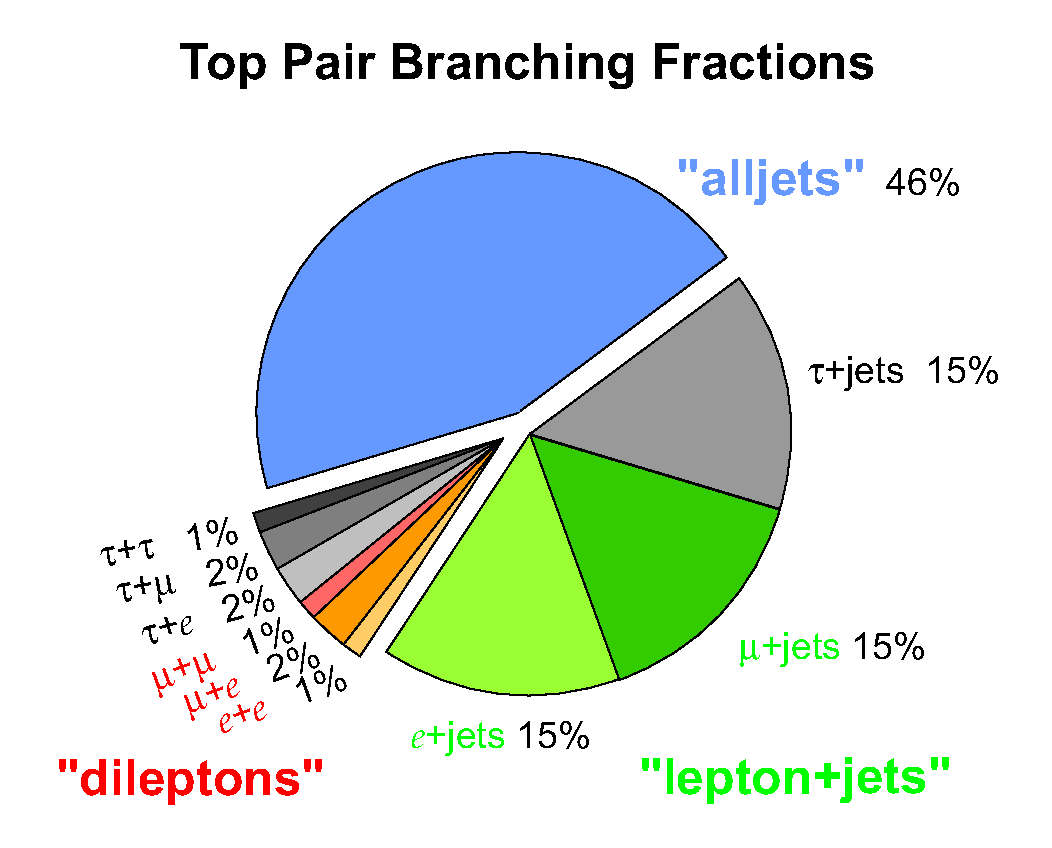
\includegraphics[width=0.6\linewidth]{figures/top_pair_branching_frac.eps} 
   \caption[Branching fractions of top-pairs.]{Branching fractions of top-pairs decaying fully-hadronically (`alljets'), fully-leptonically (`dileptons') and semi-leptonically (`lepton+jets') \cite{D0}. }
  \label{topcake}                                     
 \end{center}
\end{figure}
%
Tau leptons have various decay modes, which can be categorized by the number of charged particles involved in the decay. Main decay modes for taus include one charged particle (`1-prong') and three charged particles (`3-prong') in the decay. They are shown in table \ref{taudecays} for $\tau^-$. Here $h^{\pm}$ are charged pions $\pi^\pm$ and Kaons $K^\pm$, `neutrals' are photons $\gamma$ or neutral pions $\pi^0$. The decay modes of the $\tau^+$ can be inferred by having corresponding decay products with opposite charges.\par
Signal and background studies with various objects in the final state depend crucially on the purity of the signatures left in the detector (cf. chapter \ref{detectorsignatures}) and how they are traced back to the potential LQ. For example electrons and muons can be reconstructed reliably from their corresponding detector signatures (see chapter \ref{detectorsignatures}). Therefore the dileptonic and semi-leptonic decay modes of the top quark-pair are good candidates to study the signal and background contributions for the search of LQ. A pair of LQ provide, in addition to the hadronic $\tau$ final states, two leptons from the top-pair decay or one lepton and one jet respectively. In the face of high contributions from underlying QCD events, resulting in jet objects, dileptonic and semi-leptonic modes are more accurately to reconstruct compared to the full hadronic decays with jets only in the final state. In order to optimize the LQ signal selection the reconstruction efficiencies and fake rates of hadronically decaying taus is investigated in the $t\tau^{-}+\bar{t}\tau^{+}$ channel.
%
\begin{table}[htbp]
		\centering
                %\renewcommand{\arraystretch}{1.0}       
		\begin{tabular*}{\linewidth}{@{\extracolsep{\fill}}clc}
		\hline
		\hline
		&\textbf{mode}&  \textbf{fraction }$\Gamma_i/\Gamma$
		\\
		\hline
                \multicolumn{3}{c}{\textbf{1-prong decay}}
                \\
                $\Gamma_1$       & particle$^-\geq$ 0 neutrals $\geq 0K_L^0\nu_\tau$ & $\SI{84.58\pm0.06}{\percent}$
                \\
                $\Gamma_2$       & $\qquad \mu^-\bar{\nu}_\mu\nu_\tau$               & $\SI{17.39\pm0.04}{\percent}$
                \\
                $\Gamma_3$       & $\qquad e^-\bar{\nu}_e\nu_\tau$                   & $\SI{17.82\pm0.04}{\percent}$
                \\
                $\Gamma_4$       & $\qquad h^-\nu_\tau$                             & $\SI{11.51\pm0.05}{\percent}$
                \\
                $\Gamma_5$       & $\qquad h^-\geq 1\pi^0\nu_\tau$ (excluding $K^0$)  & $\SI{36.51\pm0.09}{\percent}$
                \\
                $\Gamma_6$       & $\qquad\qquad h^-\pi^0\nu_\tau$                   & $\SI{25.93\pm0.09}{\percent}$
                \\
                $\Gamma_7$       & $\qquad h^-\geq 2\pi^0\nu_\tau$                  & $\SI{10.81\pm0.09}{\percent}$
                \\
                $\Gamma_8$       & $\qquad\qquad h^-2\pi^0\nu_\tau$                   & $\SI{9.48\pm0.10}{\percent}$
                \\
                \hline
                \multicolumn{3}{c}{\textbf{3-prong decay}}
                \\
                $\Gamma_{9}$    & $h^-h^-h^+ \geq 0\,\text{neutrals}\geq 0K_L^0\nu_\tau$ & $\SI{15.21\pm0.06}{\percent}$
                \\
                $\Gamma_{10}$    & $\qquad h^-h^-h^+ \geq 0\,\text{neutrals}\,\nu_\tau$ (ex. $K_S^0\rightarrow \pi^+\pi^-$)      & $\SI{14.55\pm0.06}{\percent}$
                \\
                $\Gamma_{11}$    & $\qquad h^-h^-h^+\nu_\tau$                          & $\SI{9.80\pm0.05}{\percent}$
                \\
                $\Gamma_{12}$    & $\qquad \pi^-\pi^+\pi^-\nu_\tau$                          & $\SI{9.31\pm0.05}{\percent}$
                \\
                $\Gamma_{13}$    & $\qquad h^-h^-h^+\geq 1\pi^0\nu_\tau$ (excluding $K^0$) & $\SI{5.09\pm0.05}{\percent}$
                \\
                $\Gamma_{14}$    & $\qquad\qquad h^-h^-h^+\pi^0\nu_\tau$                 & $\SI{4.76\pm0.05}{\percent}$
                \\
                $\Gamma_{15}$    & $\qquad\qquad \pi^-\pi^+\pi^-\pi^0\nu_\tau$           & $\SI{4.57\pm0.05}{\percent}$
                \\
		\hline
		\hline
		\end{tabular*}
		\caption[Main decay modes of $\tau^-$.]{Main decay modes of $\tau^-$ including one charged particle (`1-prong') and three charged particles (`3-prong'). $h^{\pm}$ are charged pions $\pi^\pm$ and Kaons $K^\pm$, `neutrals' are photons $\gamma$ or neutral pions $\pi^0$. The decay products of $\tau^+$ have opposite charges correspondingly. \cite{PhysRevD}}
\label{taudecays}
%\renewcommand{\arraystretch}{1}
\end{table}
%
%%%%%%%%%%%%%%%%%%%%%%%%%%%%%%%%%%%%%%%%%%%%%%%%%%%%%%%%%%%%%%%%%%%%%%%%%%%%%%%%%%%%%%%%%%%%%%%%%%%%%%%%%%%%%%%%%%%%%%%%%%%%%
\chapter{Experimental setup for the search for scalar leptoquarks}\label{experiment}
For the search for scalar leptoquarks the {\ATLAS} detector at the Large Hadron Collider ({\LHC}) is used as experimental setup, which will be described within this chapter. The general setting of the proton-proton collider located at the {\CERN} research center is the topic of section \ref{LHC}. The particle detection of the resulting collision events, taking place in the {\ATLAS} detector with its different specialized components (section \ref{ATLAS}). Section \ref{LQpp} addresses the possible leptoquark pair production in proton-proton collisions.  
%%%%%%%%%%%%%%%%%%%%%%%%%%%%%%%%%%%%%%%%%%%%%%%%%%%%%%%%%%%%%%%%%%%%%%%%%%%%%%%%
\section{The Large Hadron Collider accelerator complex}\label{LHC}
The {\CERN} (Conseil Europ\'{e}en pour la Recherche Nucl\'{e}aire) research center was founded in $1954$ and is located near Geneva, Switzerland. It became a major European joint venture on elementary and nuclear particle physics. Currently, $22$ member states are participating in that large-scale project. The scientific ambition is manifold and includes to probe the essential constituents of nature and the fundamental forces acting between them. \cite{CERNabout}\par
%
\begin{figure}[htbp]                                 
 \begin{center}                                       
  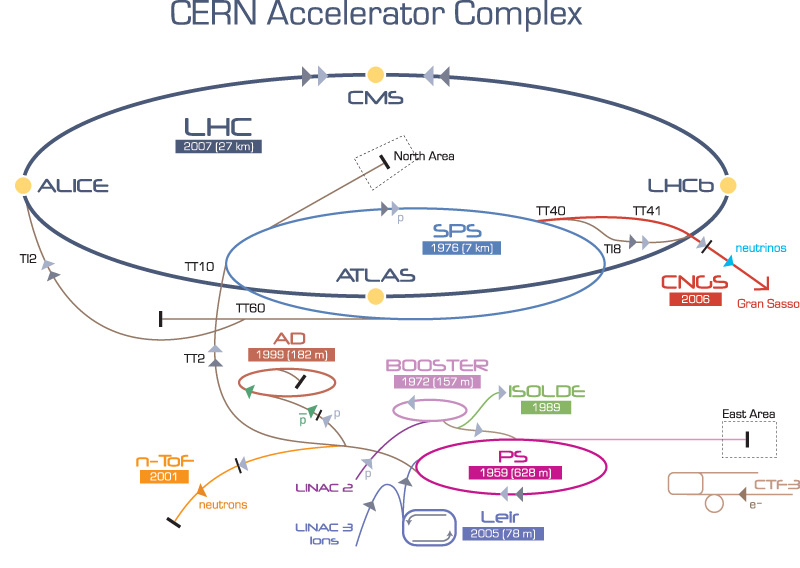
\includegraphics[width=0.8\linewidth]{figures/CERNKomplex2.jpg} 
   \caption[Schematic of the {\CERN} accelerator complex.]{Schematic of the {\CERN} accelerator complex with its different stages and few experiments like {\ATLAS} located at the interaction points of the {\LHC}. \cite{CERNKomplex}}
  \label{complex}                                     
 \end{center}
\end{figure}
%
In the accelerator complex protons reach energies of $\SI{6.5}{\tera\electronvolt}$ by going through different accelerator stages and are brought to collisions at defined interaction points in time intervals of $\SI{25}{\nano\second}$. Particle detectors, which are positioned at these interaction points, then register signatures of the resulting collision events and the analysis of newly created particles gives insight to the nature of elementary particle physics.\cite{LHCJINST}\newline
The {\LHC} is designed as two-ring proton-proton collider. It is also possible to collide lead ions. These ion collisions are provided for the {\ALICE}\cite{ALICE} experiment. However, the {\ATLAS} and {\CMS} experiment are in principle also capable of measuring lead collisions, but currently they are focused mainly on proton events. Figure \ref{complex} shows the different acceleration stages of the {\LHC} among other {\CERN} experiments.\newline
A hydrogen bottle is the starting point of the proton injection and acceleration. Fully ionized by an electron gun in chambers the protons are guided with electric fields towards the first acceleration stages. Radiofrequency (RF) cavities are responsible for the proton acceleration. Moreover the protons are accelerated in packages, known as bunches. \cite{LHCJINST}\cite{LHCSchule} Starting from the injection, protons will gain a kinetic energy of $\SI{50}{\mega\electronvolt}$ in the linear accelerator {\LINAC}2 and will be further transferred to the Proton Synchrotron Booster ($\SI{1.4}{\giga\electronvolt}$), the Proton Synchrotron ($\SI{25}{\giga\electronvolt}$), the Super Proton Synchrotron ($\SI{450}{\giga\electronvolt}$) and finally to the {\LHC} ring with its $\SI{26.7}{\kilo\meter}$ circumference. \cite{CERNabout} Dipole magnets are responsible for directing the protons through the stages and keep them on closed paths. Quadrupole magnets focus the beam to compensate the repulsive forces between the particles and to ensure small beam diameters at the interaction points for high collision rates. Conditions for a stable proton beam are diverse, including high vacua of $\SI{E-10}{\milli\bar}$ to $\SI{E-11}{\milli\bar}$ to avoid collisions with gas atoms and temperatures of $\SI{1.9}{\kelvin}$ for the superconducting NbTi-magnets of the accelerator. \cite{LHCJINST}\cite{LHCSchule}\par
Different experiments like \ALICE\cite{ALICE}, {{\LHC}}b\cite{LHCb} are located at the {\LHC} due to the variety of research questions. The general-purpose detectors {\ATLAS} and its counterpart {\CMS}\cite{CMS} are specialized to high luminosities\footnote{For the physical definition see eq. (\ref{Lumi}).}, exploiting the large range of physics opportunities made possible by the {\LHC}. Main tasks of the {\ATLAS} experiment are precision measurements of the SM (see chapter \ref{SM}), a better understanding of Quantum Chromo Dynamics (QCD) and the search for supersymmetric models, and new physics, among others. With the {\LHC} collision rate of $10^9$ inelastic events per second, up to $23$ simultaneous events per bunch-crossing at dominating high QCD cross sections require a powerful detector that is capable of recognizing the characteristic signatures. These circumstances are the reasons for the demands on the {\ATLAS} detector, including fast electronic elements, high detector granularity, handling high particles fluxes and reducing overlapping events at a large acceptance and coverage region. \cite{ATLASJINST}       
%AußerdeM: Hinweis auf high Lumi LHC als Art mini-Ausblick in diesem Kapitel https://arxiv.org/pdf/1705.08830.pdf, https://cds.cern.ch/record/1711887/files/ATL-COM-UPGRADE-2014-014.pdf ################
%%%%%%%%%%%%%%%%%%%%%%%%%%%%%%%%%%%%%%%%%%%%%%%%%%%%%%%%%%%%%%%%%%%%%%%%%%%%%%%%%%%%%%%%%%%%%%%%%%%%%
\section{The ATLAS detector at the LHC}\label{ATLAS}
One of the general purpose detectors for proton-proton collisions is the {\ATLAS} detector. This $\SI{25}{\meter}$ tall detector is located at one interaction point of the {\LHC} where bunches, consisting of approximately $\SI{E11}{}$ protons, collide at a rate of $\SI{40}{\mega\hertz}$ \cite{ATLASJINST}. The number of particles encountered per time is given by \cite{Perkins}
\begin{align}
                        \dot{N}=\mathcal{L}\sigma
\end{align}
with the cross section $\sigma$ for the present event and the instantaneous luminosity $\mathcal{L}$. The luminosity depends only on the characteristics of the collider and is often used as key parameter in collider physics \cite{LHCJINST}.
\begin{align}
                        \mathcal{L}=\frac{N_bn_bf_{\text{rev}}\gamma_r}{4\pi\epsilon_n\beta^*}F
\label{Lumi}
\end{align}
Where $N_b$ is the number of particles per bunch, $n_b$ the number of bunches per beam, $f_{\text{rev}}$ the rotational frequency, $\gamma_r$ the Lorentz factor, $\epsilon_n$ the normalized transverse beam emittance, $\beta^*$ the betatron function at the collision point and $F$ respects the geometric luminosity reduction factor due to the crossing angle at the collision point. The luminosity measured at the {\ATLAS} interaction point exceeded the design luminosity of $\mathcal{L}=\SI{2.05E34}{\per\square\centi\meter\per\second}$ by a factor of $2.05$ on the $2^{\text{nd}}$ of November 2017, proving the great success of the {\LHC} machine setup over the years \cite{designLumiExceeded}.\par 
%Erklärung für Lumi auch aus Perkins? ##########
To meet the requirements of a general-purpose detector, several considerations for the detector design were taken into account: On the one hand there is the demand to be sensitive to the great variety of particles governed by the fundamental forces (see chapter \ref{SM}). On the other hand the yet unknown physics should be potentially covered as well by the {\ATLAS} detector -- all seen from the angle of performing precision measurements. 
%Motivation eher sogar von der Seite, wieso so gebaut, wie er ist --> Teilchen detektieren (Verweis auf SM Kaptiel)-> Schichtaufbau-> etc... #######
The basic structure of {\ATLAS} is shown in figure \ref{ATLASandCoordinate} with its different sub-detector systems together with the convention for the coordinate system.  %Koordinatensystem
%
\begin{figure}
 \centering
  \begin{subfigure}[c]{0.95\textwidth}
   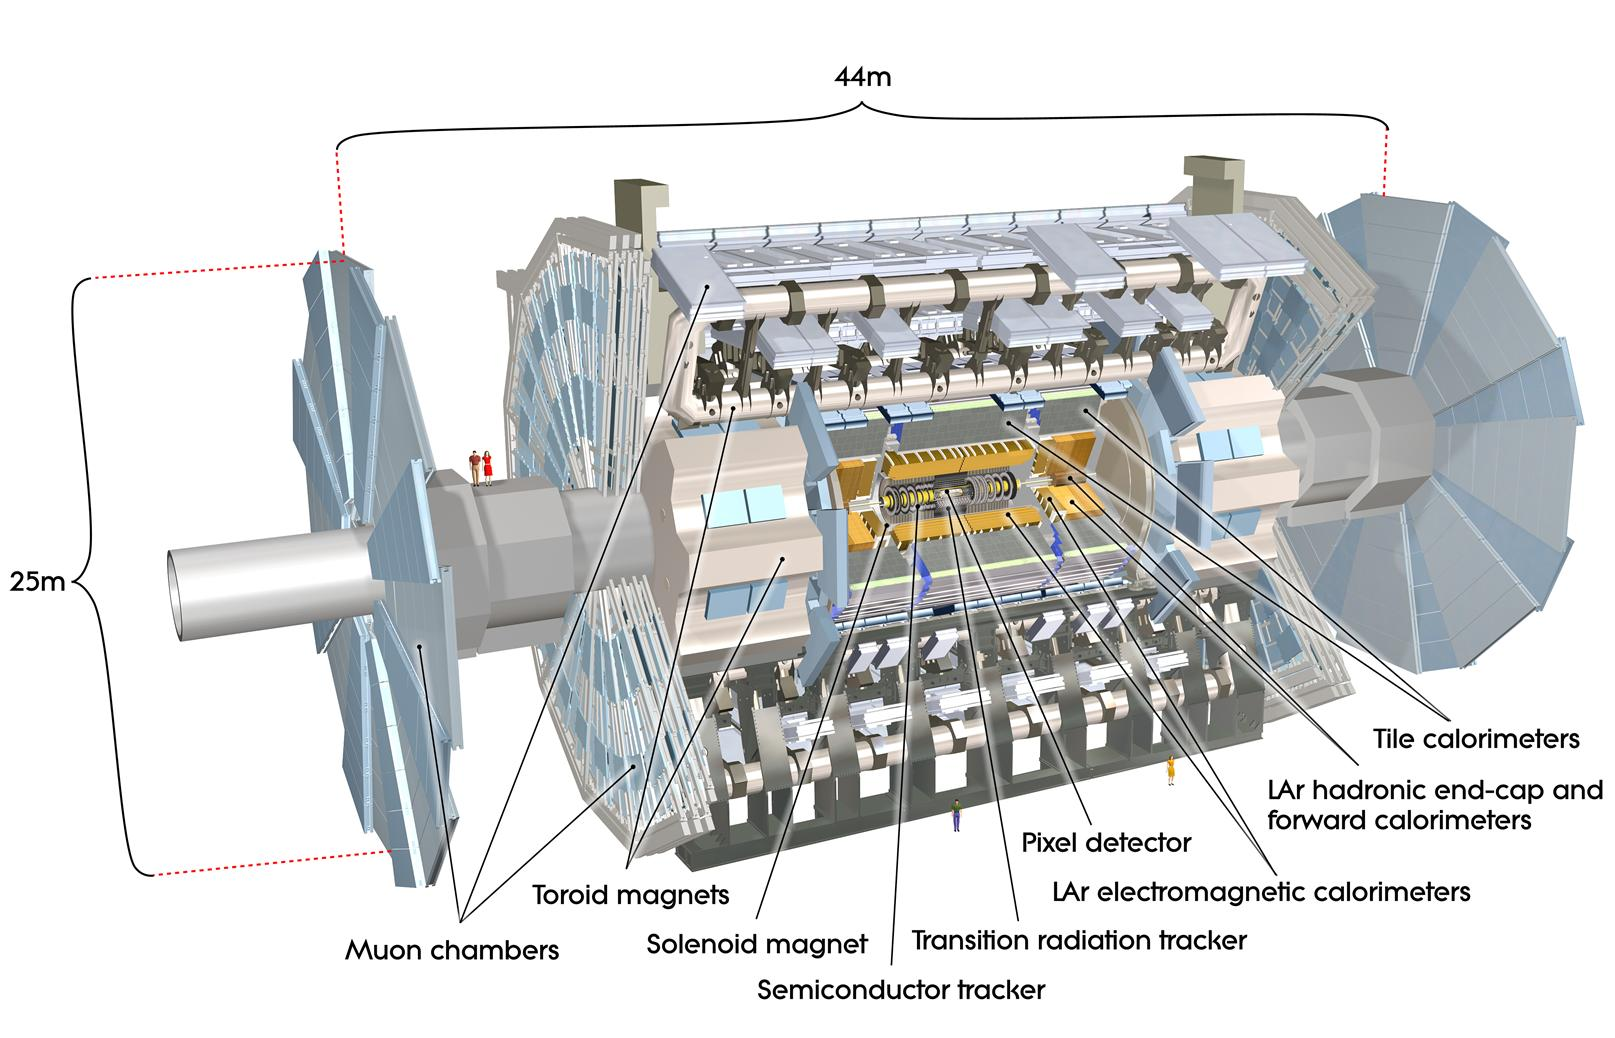
\includegraphics[width=\textwidth]{figures/ATLASDesign.png}
    \subcaption[The structure of the {\ATLAS} detector and its sub-systems.]{The layered structure of the {\ATLAS} detector at the {\LHC} with its sub-systems inner detector, calorimeter, magnets and muon spectrometer \cite{ATLASJINST}.}
   \label{ATLASDesign}
  \end{subfigure}
  \begin{subfigure}[c]{0.95\textwidth}
   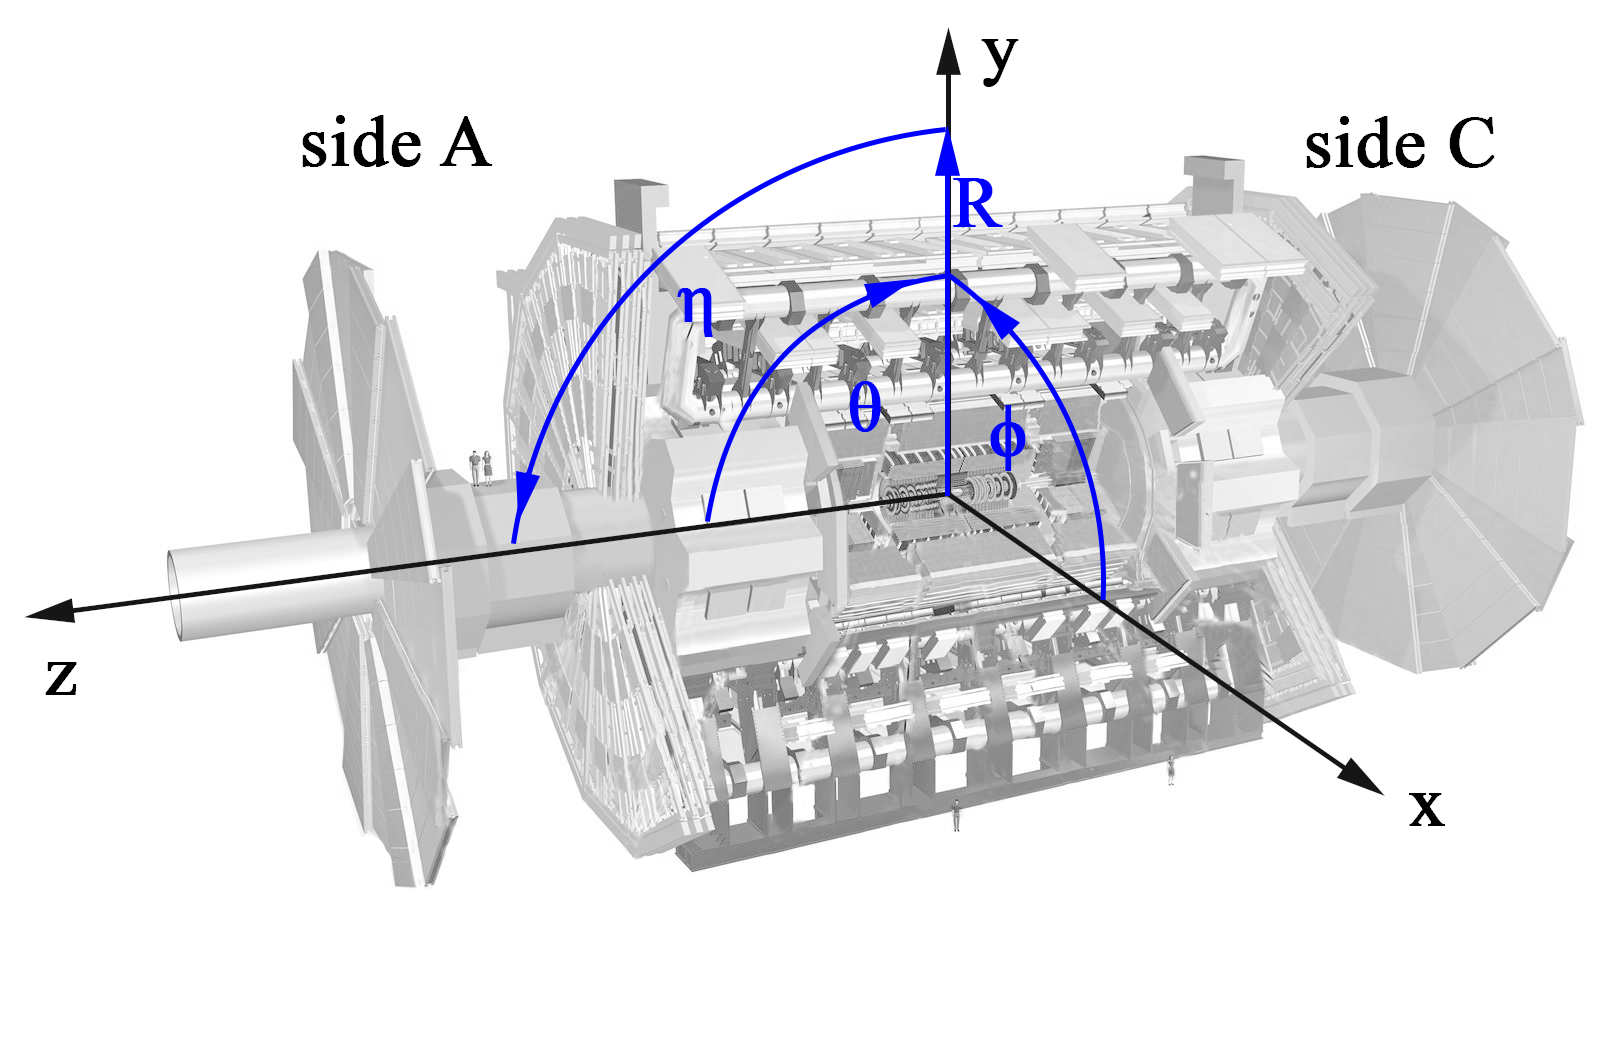
\includegraphics[width=1\textwidth]{figures/ATLASDesignCoordinate.png}
   \subcaption[Definition of the global {\ATLAS} coordinate system.]{The global {\ATLAS} coordinate system formulated in cylindric coordinates with the $z$-axis parallel to the beam line and the transverse plane defined through azimuthal angle $\phi$ and pseudorapidity $\eta$. Based on \cite{ATLASJINST}.}
   \label{Coordinate}
  \end{subfigure}
 \caption[Structure of the {\ATLAS} detector and the coordinate system.]{Structure of the {\ATLAS} detector and the coordinate system.}
 \label{ATLASandCoordinate}
\end{figure}
%
The nominal interaction point acts as origin of the coordinate system, where the $z$-axis follows the beam line counterclockwise. Perpendicular to the $z$-axis lies the transverse $x$-$y$-plane usually described through the azimuthal angle $\phi$. The positive $x$-axis points towards the center of the {\LHC}. The cylindric symmetry of the detector suggests a cylindric coordinate system with the angle $\theta$ starting from the beamline. \cite{ATLASJINST} Since the polar angle is not a Lorentz invariant quantity, it is useful to describe the position in terms of rapidity \cite{LHCJINST} $w=\frac12\ln{\frac{E+p_zc}{E-p_zc}}$ in that highly relativistic regime. In the limit of large momenta, i.e. $|\mathbf{p}|c\approx E$, the rapidity coincides with the pseudorapidity formulated as \cite{ChinaPseudorapidityBook}
\begin{align}
                        \eta=-\ln{\tan\frac{\theta}{2}}\text{.}
\label{pseudorapidity}
\end{align}
This variable only depends on the polar angle is therefore the adequate quantity in the context of collision experiments, where usually the angle $\theta$ from the beamline is measured. \cite{ChinaPseudorapidityBook}\par
The collision products, originating from the interaction point at the center of the {\ATLAS} detector, will propagate through the different layers of the detector's sub-systems. The inner detector is responsible to track electrically charged particles. The magnetic fields for identifying the particles' electric charge and for momentum measurement is provided by the {\ATLAS} magnet system. The next layer includes the calorimeter. The electromagnetic calorimeter measures mainly the energy deposit of electrons, positrons and photons and allows the distinction between them with the help of the track information given by the inner detector. Hadronic particles will deposit their energy in the hadronic calorimeter. The outermost layer consists of the muon system responsible for a second independent measurement of the muon and anti-muon tracks. \cite{ATLASJINST}\par    
\textbf{The magnet system} includes a superconducting solenoid with a field strength of $\SI{2}{\tesla}$ surrounding the inner detector as well as three large superconducting toroid magnets composed in an eight-fold azimuthal symmetry around the calorimeter. The barrel toroid magnet delivers a field strength of $\SI{0.5}{\tesla}$ and in the end-cap a field of $\SI{1}{\tesla}$ is present. \cite{ATLASJINST}\newline%Bending particle path -->identification... ######
\textbf{The inner detector} is responsible for momentum measurements, vertex measurements and pattern recognition for the identification of electrically charged particles. This is achieved with a combination of semiconductor pixel and microstrip trackers (SCT). The Insertable B-Layer (IBL) is the innermost layer of the pixel detectors at a radius of $\SI{3.3}{\centi\meter}$ away from the beam line. Additional straw tube tracking detectors are sensitive to transition radiation (TRT) located in the outer part that are responsible for high vertex and momentum resolution. The $R-\phi$ segmented pixel detectors are of a size of $50\times \SI{400}{\square\micro\meter}$ and the SCTs with their $8$ strip layers cover together a range of $|\eta|<2.5$. Typically $36$ hits per track are provided by the $\SI{4}{\milli\meter}$ straw tubes of the TRTs, which cover the range $|\eta|\leq 2.0$. \cite{IBL}\cite{ATLASJINST}\newline %Unterscheidung teilchen anhand der Übergangsstrahlung ####################
Liquid argon electromagnetic sampling \textbf{calorimeters} with high granularity allow for an excellent energy measurement of electrons and photons. They have a total thickness of more than $22$ radiation lengths $X_0$ in the barrel region ($|\eta|<1.475$) and more than $24X_0$ in the end-cap region ($1.375<|\eta|<3.2$). For hadronic energy measurements a scintillator-tile calorimeter covering $|\eta|<1.7$ is in operation. It is a sampling calorimeter and uses steel as absorber material and scintillating tiles as active material in conjunction with wavelength shifting fibres. Further LAr technology is used for hadronic particles in the outer pseudorapidity range up to $|\eta|=3.2$. Here copper plates provide the absorber material. The forward calorimeters extend the coverage of hadronic and electromagnetic energy measurements to $|\eta|=4.9$ and are $10X_0$ deep. \cite{ATLASJINST}\newline%Energiemessung: provide god res for high energy jets###################
The \textbf{muon system} is located in the outer layer of the {\ATLAS} detector and provides resolution for high energy muon tracks with three layered precision chambers up to the range of $|\eta|<2.7$. This is possible because of the air-cored toroid magnet system including one barrel and two end-cap magnets generating strong bending power in a large volume and delivering  a mostly perpendicular magnetic field with respect to the muon trajectories. The bending power $\int{\vec{B}d\vec{l}}$ along the track of the muon $d\vec{l}$ reaches from $\SI{1.5}{\tesla\meter}$ to $\SI{5.5}{\tesla\meter}$ in the range $|\eta|<1.4$ (barrel) and up to $\SI{7.5}{\tesla\meter}$ (end-cap). The precision chambers are Monitored Drift Tubes (MDT) and in the larger pseudorapidity range Cathode Strip Chambers (CSC), which are multiwire proportional chambers. Due to the fact that the overall performance crucially depends on the alignment of the muon detectors with respect to each other and with respect to the inner detector, MDTs are equipped with a optical monitoring system with $12000$ sensors. Resistive Plate Chambers (RPC) and Thin Gap Chambers (TGC) are the constituents of the muon trigger system. \cite{ATLASJINST} \newline %Myonen kommen überall durch-->hier detektieren + Problem der Spurkrümmung für high pt--> eigenes system für die genauere myon-messung ############
Due to technology and resource limitations the data recording rate has to be reduced from $\SI{40}{\mega\hertz}$ to $\SI{1}{\kilo\hertz}$. This poses high demands on an efficient \textbf{trigger system} which is organized in two levels. This is the level $1$ hardware-based trigger and the software-based high level trigger (HLT). Level $1$ uses only a subset of the total detector information making basic decisions to flag so called regions of interest within the detector's coordinate system. Searches include patterns for high transverse momenta of muon tracks, electrons and photons as well as jets or large missing energy balances. The output rate after this first selection accounts for $\SI{100}{\kilo\hertz}$. The HLT is responsible for selecting the level $1$ triggered regions at full granularity and precision, reconstructing the complete events. This event filter is the final stage and achieves data reduction down to the final data-taking rate of $\SI{1}{\kilo\hertz}$, writing events of the size of approximately $\SI{2.4}{\giga\byte\per\second}$ to the disks. The HLT selection criteria are implemented using offline analysis procedures. \cite{ATLASJINST}\cite{newATLASJINST} %efficient triggering with sufficient background rejection ###############
% XXXXXXXXXXXXXXXXXXXXXXXXXXX alte Version XXXXXXXXXXXXXXXXXXXXXXXX
%three levels. Level $1$ uses only a subset of the total detector information making basic decisions to flag so called regions of interest within the coordinate system. Searches include patterns for high transverse momenta of muon tracks, electrons and photons as well as jets or large missing energy balances. The output rate after this first selection accounts for $\SI{75}{\kilo\hertz}$. The high level trigger $2$ and $3$ are responsible for selecting the level $1$ triggered regions at full granularity and precision. The level $3$ event filter is the final stage and achieves data reduction down to the final data-taking rate of $\SI{200}{\hertz}$, writing events of the size of approximately $\SI{1.3}{\mega\byte}$ to the disks. The event filter's selection criteria are implemented using offline analysis procedures. \cite{ATLASJINST}
%%%%%%%%%%%%%%%%%%%%%%%%%%%%%%%%%%%%%%%%%%%%%%%%%%%%%%%%%%%%%%%%%%%%%%%%%%%%%%%%%%%%%%%%%%%%%%%%%%%%%%%%
\chapter{Turning detector signatures into physical objects}\label{detectorsignatures}
All components of the detector system of {\ATLAS} (see chapter \ref{ATLAS}) deliver electronic signals of the proton-proton collisions, which have to be reconstructed to physical objects for the analysis. This chapter describes the reconstruction of the physical objects like electrons, muons, jets and b-flavor jets and taus, which are relevant to the analysis in this thesis. Furthermore, the role of Monte Carlo simulations in the analysis is presented briefly.
\section{Electron reconstruction at ATLAS}\label{eReconstruction}
Electrons and positrons are stable and abundant final states of collision products. Therefore, relying on signatures of such particles in the detector is essential. Electrons and positrons\footnote{In this section, the term `positron' is absorbed in the term `electron'.} give rise to tracks in the inner detector and deposit their total energy in the electromagnetic calorimeter. The tracks and calorimeter signals are used for the electron reconstruction. \cite{ePerformance}\par
For the reconstruction of electrons in the central region ($|\eta|<\SI{2.47}{}$) several steps are necessary. At first, with respect to the granularity of the calorimeter, it is searched for electron cluster seeds in the so called step of \textit{seed-cluster reconstruction}. For more information on clusters see section \ref{jets}. The efficiency of this search is $\SI{95}{\percent}$ to $\SI{99}{\percent}$ for transverse energies up to $\SI{7}{\giga\electronvolt}$ and $>\SI{15}{\giga\electronvolt}$ respectively. The \textit{track reconstruction} is responsible for the pattern recognition in the inner detector taking into account the energy loss due to mainly bremsstrahlung in the detector material of up to $\SI{30}{\percent}$. The track seed, consisting of at least three hits in different layers of the silicon detectors, is extended to a full track of at least seven hits and is extrapolated to the regions of interest at the electromagnetic calorimeter. This is done by the {\ATLAS} Global $\chi^2$ Track Fitter \cite{trackfitter}. Afterwards a loose matching of the tracks to the clusters in the electromagnetic calorimeter is done in the \textit{electron specific track fit}. The final step, \textit{electron candidate reconstruction}, is the selection of the final track candidate out of the different tracks with the best matching to the initial cluster seed. \cite{ePerformance}\newline
Both, the information of the track and the energy cluster, are used for the four-momentum calculation of the electrons. Algorithms for reconstructed electron identification are applied to distinguish signal-like or background-like electron candidates. For that the TRT likelihood method plays an important role, which uses the high-threshold hits of each TRT. Several discriminating variables are evaluated\footnote{For further details see \cite{ePerformance}} for this likelihood method (LH). Based on the outcome, three quality categories for the electron identification are defined: \textit{Loose} relies on information of the hadronic calorimeter and the first two layers of the electromagnetic calorimeter. \textit{Medium} adds information from the TRTs, the transverse impact parameter and the third layer of the electromagnetic calorimeter, whereas the \textit{Tight} operating point additionally considers track-cluster matching variables like the ratio of the cluster energy over the track momentum. \cite{ePerformance}\newline
For a well reconstructed electron additional requirements on the isolation of the cluster and the track need to be met. In this thesis the definition of the operating point \textit{Gradient} is relevant. The efficiency depends linearly on the transverse energy $E_T$. For Gradient the isolation efficiency used in the operating point optimization is $\SI{0.1143}{\percent\per\giga\electronvolt}\cdot E_T+\SI{92.14}{\percent}$ for the calorimeter cluster and the track. \cite{ePerformance}\newline
The high level electron trigger has a transverse energy threshold of at least $\SI{24}{\giga\electronvolt}$ and requires at least a medium quality electron based on the likelihood categories described in section \ref{eReconstruction} (\texttt{e24\textunderscore lhmedium}). This high level trigger (HLT) is seeded from the electromagnetic calorimeter of the level 1 trigger system with a threshold of at least $E_T<\SI{20}{\giga\electronvolt}$ (\texttt{L1EM20VH}). Additionally a energy dependent veto against energy deposits in the hadronic calorimeter behind  the electromagnetic cluster is implemented. Thus it acts as hadronic veto (denoted with `\texttt{H}'). Furthermore the transverse energy threshold depends slightly on the pseudorapidity to compensate for energy losses in the material directly in front of the electromagnetic calorimeter (denoted with `\texttt{V}'). The next step of a tighter trigger selection includes a transverse energy threshold of $E_T>\SI{60}{\giga\electronvolt}$ and requires a medium quality electron (\texttt{e60\textunderscore lhmedium}). Adapted for high energy electrons the trigger \texttt{e120\textunderscore lhloose} provides electrons with transverse energies of at least $\SI{120}{\giga\electronvolt}$ by requiring at the same time the loose electron working point. \cite{trigger:e:mu} The above electron trigger menu is valid for data taken in 2015. For the data-taking periods in 2016-2018 the following changes are applied:\newline
HLT thresholds are set to $\SI{26}{\giga\electronvolt}$ with the tight quality requirement (\texttt{e26\textunderscore lhtight}) and a variable cone size isolation (\texttt{ivarloose}), which uses the criteria that the sum of the track momentum must not exceed $\SI{10}{\percent}$ of the electron's transverse energy within a cone of $\Delta R=\sqrt{\Delta\eta^2+\Delta\phi^2}<0.2$ \cite{trigger:ivarloose:erkl}\cite{trigger:ivarloose:form}. Additional to that no transverse impact parameter cut is applied (\texttt{nod0}) \cite{trigger:ivarloose:erkl}. The complementary trigger for the high transverse energy regime is increased to $\SI{140}{\giga\electronvolt}$ \cite{trigger:e:mu}.
%electron identification starts from searches of the highest energy deposit in the second layer of em, immer unter dem Aspekt möglichst schneller processierung       
%lowest single e trigger e24_lhmedium threshold of ET>24GeV + medium LH identification of the electron
%seeded from the electromagnetic calorimeter at level 1 with threshold ET>20GeV L1EM20VH
%energy dependent veto against energy deposited in the hadronic calorimeter behind the electronmagnetic cluster = hadronic veto H
%ET threshold slighly eta dependent to compensate for energy loss in the passive material in front of the calorimeter V
%complementary trigger for the high transverse energy regime which requires a loose electron identification with ET>120GeV
%---------------cite trigger:e:mu
%nod0 -> no transverse impact parameter cut is applied
%iloose indic       ates a variable cone size isolation requ
%----------cite trigger:ivarloose:erkl
%iloose            track momentum sum can not be more than  10% of the electron transverse energy within dR<0,2
%------------------cite trigger:ivarloose:form
%
%
%
%
\section{Muon reconstruction at ATLAS}\label{muReconstruction}
Muons are good tracers of particles with shorter lifetimes and thus should be reconstructed as an important information carrier of the particle collisions. Muons\footnote{In this section, the term `anti-muon' is absorbed in the term `muon'.} are reconstructed independently in the inner detector and the muon spectrometer and the resulting combination of the two gives the full muon track. \cite{muPerformance}\par
The first reconstruction step is again pattern recognition for seeds in the silicon layers from the inside towards the outside of the inner detector. Seeds are formed out of three space points. The space points are provided by the pixel detectors with their local two-dimensional space points and from the combination of a pair of SCTs. The default setting of the seeding algorithm allows three combinations for space points: all space points within the pixel detector, all within the SCTs or two within the pixel detector and one within the SCT. \cite{muInner}\newline
The muon reconstruction in the muon spectrometer is initiated by the search for hit patterns in the muon chambers to form segments. Muon track candidates are created by fitting the segments from different layers, which is done by a combinatorial search. Selection criteria include hit multiplicity and fit quality to find the optimal track. The hits associated to each track candidate, after applying an overlap removal algorithm, are fitted using a global $\chi^2$ fit. \cite{muPerformance}\newline
Different types of reconstructed muons are distinguished, depending on which information of the possible muon candidate is available in the inner detector, the calorimeter and the muon spectrometer. After a first signature combination of the involved sub-detector signatures, the energy loss of the muon traveling through the calorimeters and the detector material is included in a refit. A \textit{combined muon} is reconstructed from the independent inner detector and muon spectrometer measurement in a global refit, if both sub-detector components have registered a muon signature. \textit{Segment-tagged muons} are extrapolated from the inner detector muon track to at least one local segment of the muon spectrometer. If the track of the inner detector can be matched to energy deposits in the calorimeter, the reconstructed muon is called \textit{calorimeter-tagged} muon. Muons reconstructed only on the basis of the muon spectrometer are extrapolated back to the interaction point and therefore are called \textit{extrapolated muons}.\cite{muPerformance}\newline
Quality requirements on the track suppress background contributions and guarantee a robust momentum measurement by including discriminating variables like the $\chi^2$ of the combined track. This categorization finalizes the muon identification process. For the category \textit{Loose muons} all above listed muon types are used. The category \textit{medium muons} minimizes the systematic uncertainties and is based only on combined muons and extrapolated muons. \textit{Tight muons} only uses the combined muon type and is optimized for maximum purity at the cost of some efficiency. The \textit{high-$p_T$ muons} are designed for  a maximization of the momentum resolution for tracks above $\SI{100}{\giga\electronvolt}$. \cite{muPerformance}\newline
The relevant isolation requirement used in this thesis for muons is the so called \textit{Gradient} isolation, which includes track-based and calorimeter-based discriminating variables. In this case it is the sum of transverse momenta of the tracks in a cone around the muon with $\Delta R=\sqrt{\Delta\eta^2+\Delta\phi^2}<0.3$, excluding the muon track itself. The calorimeter condition is based on the sum of transverse energies of the topological clusters around the muon in a cone of $\Delta R<0.2$. \cite{muPerformance}\cite{varcone}\newline
Trigger decisions for muons are based on the MS and the quality of the match that combines the track measurement of the MS and the ID. The requirement on the transverse momentum of the combined muon is at least $\SI{20}{\giga\electronvolt}$ with an additional loose isolation (\texttt{mu20\textunderscore iloose}). The loose isolation means that the scalar sum of the track $p_T$ values does not exceed $\SI{12}{\percent}$ of the muon's transverse momentum within a cone of $\Delta R<0.2$. This HLT is based on the decisions of the trigger level 1 seed, which selects muons with a transverse momentum of at least $\SI{15}{\giga\electronvolt}$ (\texttt{L1MU15}). The HLT trigger \texttt{mu50} has a threshold of $p_T<\SI{50}{\giga\electronvolt}$ and complements the trigger's high momentum regime without isolation conditions. The above muon trigger menu is based on the data taking periods in 2015 \cite{trigger:e:mu}. Changes to the data selection of the periods of the year 2016-2018 are as follows: \newline
The HLT transverse momentum requirement is changed to at least $>\SI{26}{\giga\electronvolt}$ and the isolation requirement is changed in such a way that the scalar sum of the track momentum must not exceed $\SI{7}{\percent}$ of the muon's transverse momentum within a cone of $\Delta R<0.3$ (\texttt{e26\textunderscore ivarmedium}) \cite{trigger:mu}.            
%MS only und quality of th e matching of muon track measured independently in the ID and MS (physical property = pT)
%pT>20GeV of CB muon candidate + loose isolation: sum of track pT values  in cone around dR<0,2 is set to <12% of the muon pT
%seeded by L1MU15 -> pT>15GeV
%complemented by mu50 withoout isolatoin for high pT muons with pT>50GeV
%---------------perf of the atlas trigger system in 2015
%ivarmedium ptrack compared to pt complett <7% in cone dR<0,3
%----------------- cite erkl
%
%
\section{Jet reconstruction at ATLAS}\label{jets}
Note that jets are not physical objects in the sense of elementary particles, but denote collimated streams of colored final states. Due to confinement (cf. chapter \ref{SM}) colored fragments will always result in jet signatures. \cite{PhysTeV}\newline  
For the reconstruction of hadronic parts of final states like isolated hadrons, jets (see also section \ref{btagging}) and hadronically decaying taus (see also section \ref{taus}), the {\ATLAS} experiment employs clusters of topologically connected calorimeter cell signals (topo-clusters). The topo-cluster algorithm analyzes the spatial distribution of the cell signals to reconstruct the energy and direction of the incoming particle. \cite{topo}\par
The segmented lateral readout of the high granularity calorimeter allows the distinction between signals from particle showers and background events with the aid of the cell signal significance $\zeta_\text{cell}^\text{EM}$. \cite{topo} Seeds are defined by cells, where the absolute energy $|E|$ exceeds the noise level by a factor of four standard deviations. The topo-clusters are expanded by iteratively adding all neighbor cells with energies two standard deviations above the noise level. \cite{jetPerformance}\newline
For this thesis the relevant clustering algorithm is the anti-$k_t$ algorithm. The algorithm is based on the following definitions \cite{antikt}:
\begin{align}
                        &d_{ij}=\min(k_{ti}^{-2},k_{tj}^{-2})\frac{\Delta_{ij}^2}{R^2}\,\text{,}\\
                        &d_{iB}=k_{ti}^{-2}\,\text{,}
\label{antiktalgorithm}
\end{align}
where $d_{ij}$ is the distance between the objects $i$ and $j$ and $d_{iB}$ the distance between $i$ and the beam $B$ in the transverse plane. $k_t$ denotes the transverse momentum and $\Delta_{ij}^2=(\eta_i-\eta_j)^2+(\phi_i-\phi_j)^2$ denotes the cone between $i$ and $j$. The radius parameter $R$ scales the distance $d_{ij}$ with respect to $d_{iB}$ that any final pair of jets $a$ and $b$ is at least separated by $\Delta^2_{ab}=R^2$. The final clustered jet is obtained by the search of the minimum in distances $d_{iB}$ and $d_{ij}$. If the minimum is $d_{ij}$, then the sum of the four-momentum of object $i$ and $j$ is calculated and is treated as a new object. Again all distances between the objects are re-calculated until $d_{iB}$ is a minimum. This means, object $i$ is the final jet. The anti-$k_t$ algorithm is a stable jet reconstruction algorithm and is not prone to fluctuations because of adding low $k_t$-objects. \cite{antikt}
%
%
\section{b-jet reconstruction at ALTAS}\label{btagging}
The third generation quarks, i.e. top (t) and bottom (b), play a crucial role in the SM and its various extension possibilities like the Leptoquark Model due to their large masses \cite{Hansson}. Therefore, it is essential to identify hadrons containing b quarks and separating them from light-flavor quarks at hadron collider detectors like {\ATLAS}. This task is commonly referred to as b-tagging and can be seen as a classification problem with the goal to assign correct jet flavors. To this end the particle tracks in the inner detector and the jet reconstruction of clusters in the electromagnetic and hadronic calorimeter are discriminating objects. \cite{Paganini}\par
%
\begin{figure}[htbp]                                 
 \begin{center}                                       
  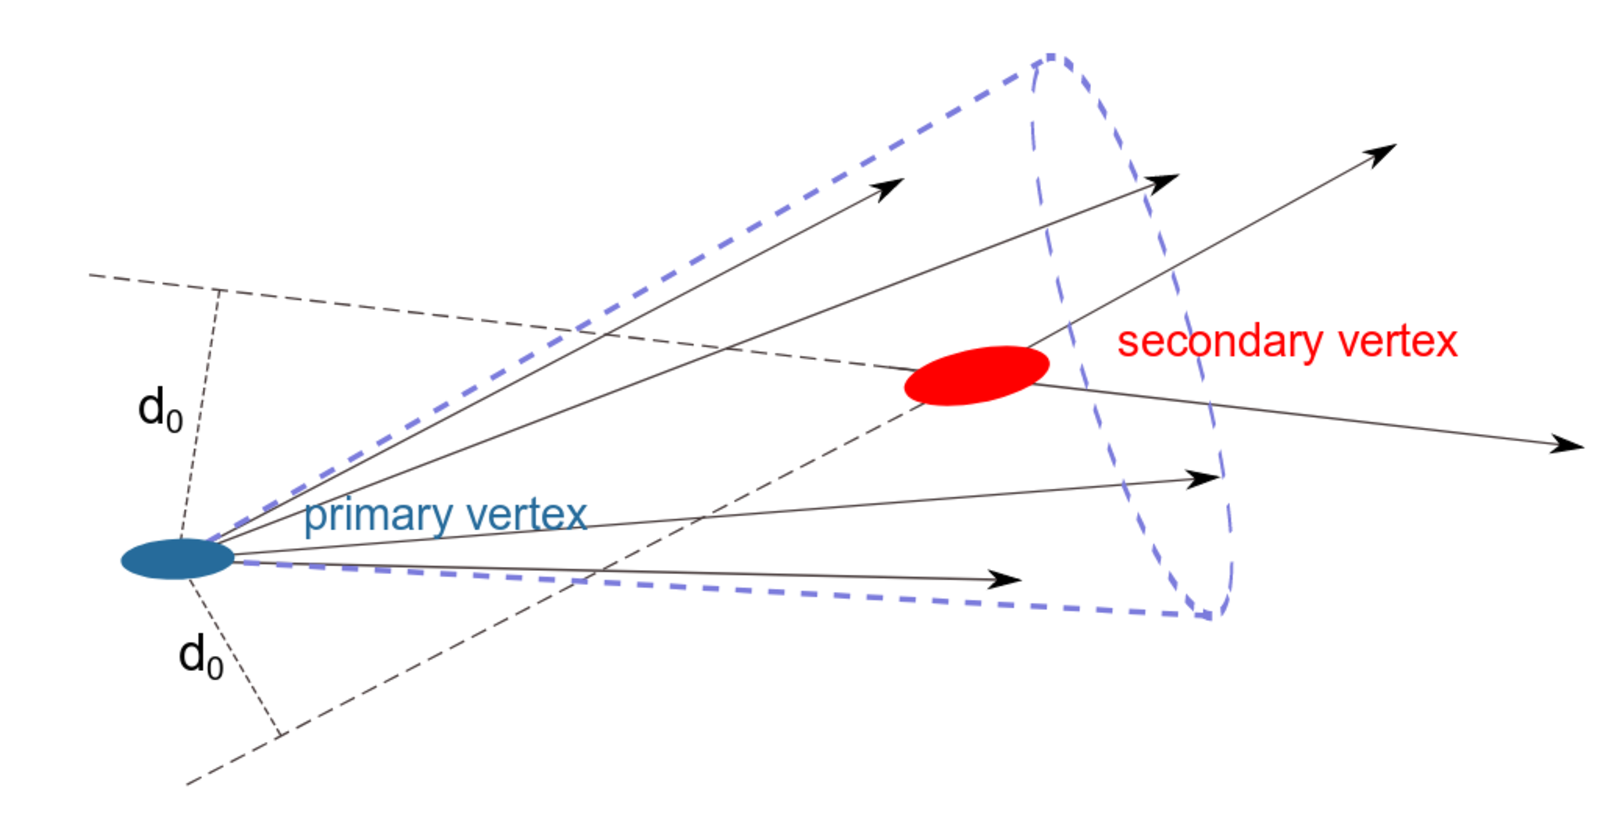
\includegraphics[width=0.55\linewidth]{figures/btagged.pdf} 
   \caption[Tracks in a b-jet.]{Signature of a b-jet with the primary and secondary vertex created relevant for b-tagging. $d_0$ is the impact parameter. \cite{Hansson}}
  \label{btagged}                                    
 \end{center}
\end{figure}
%
The long lifetime of B hadrons of $\sim\SI{1.6}{\pico\second}$ allows them to travel a few millimeters in the detector. The subsequent decay of those heavy particles within a secondary vertex produces tracks with a comparably large impact parameter $d_0$ that is the shortest distance of the particle track from the primary vertex (see figure \ref{btagged}). This signature and the deduced impact parameter significance $S(d_0)=\frac{d_o}{\sigma(d_0)}$, where $\sigma(d_0)$ is the uncertainty of the impact parameter, are used by the b-tagging algorithms including five low-level and two high-level taggers. \cite{Hansson} The b-tagging algorithms rely on multivariate combinations of the information and process them to calculate a discriminant value for each jet. Thresholds on these values define the working point to provide efficient identification of b-jets. For better information processing of the combinations of large input parameters neural network models can be used. \cite{Luca} One example for a b-tagging algorithm is the the MV2 tagger which uses 24 input variables of the low-level taggers together with kinematic properties\footnote{For further details on MV2 see \cite{MV2}}. \cite{Paganini} It uses a boosted decision tree (BDT) to discriminate b-jets from light-jets and c-jets. \cite{MV2} The light-flavor and c-jet rejection as a function of b-jet efficiency for MV2c10 (red line) is shown in figure \ref{btageff}. The description `c10' indicates the fraction of c-jet composition of the training background sample, e.g. for MV2c10 the c-jet to light-jet composition is $\SI{10}{\percent}/\SI{90}{\percent}$. Three other tagger configurations are shown in comparison as well as their ratio to MV2c10. Following the MV2c10 efficiency curve different working points can be defined. The relevant working point for the physical object selection in this work is $\SI{77}{\percent}$ (cf. chapter \ref{physObj}). The c-jet rejection rate for this working point is $6$, for light-jet rejection $134$ and for $\tau$-rejection $22$ extracted from $t\bar{t}$ events. \cite{MV2c10}    
\begin{figure}
 \centering
  \begin{subfigure}[t]{0.49\textwidth}
   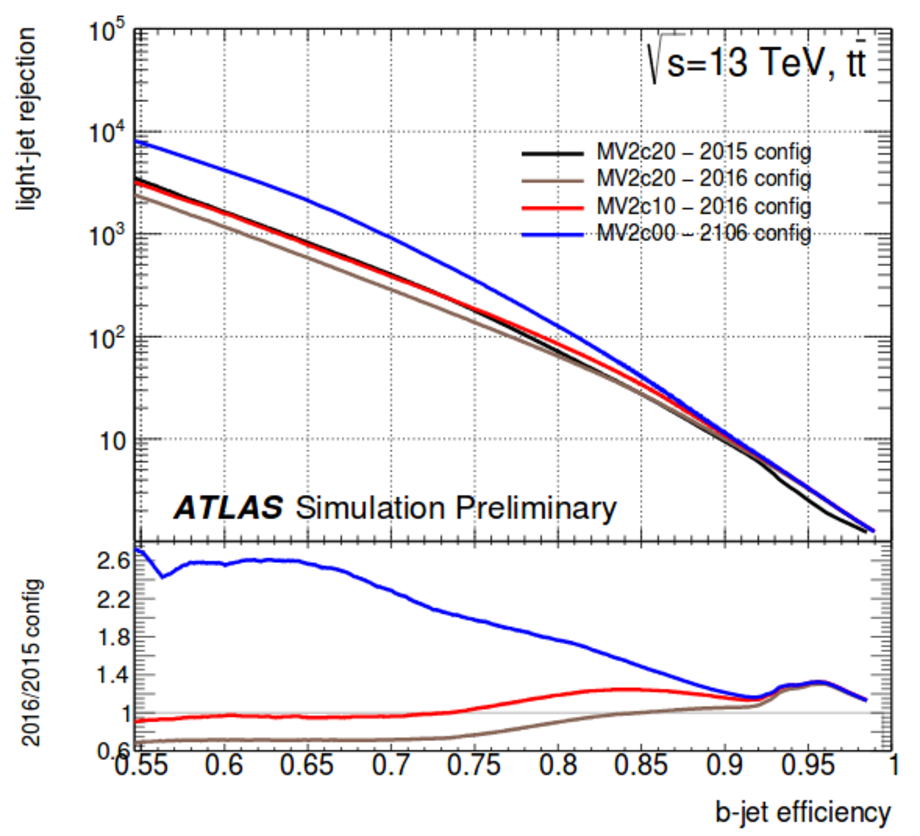
\includegraphics[width=\textwidth]{figures/lightjetrejection.pdf}
    \subcaption[Light-jet rejection versus b-jet efficiency for the MV2c10 tagger.]{Light-jet rejection versus b-jet efficiency for the MV2c10 tagger (red) in comparison to previous configurations evaluated on $t\bar{t}$ events. The ratio is evaluated with respect to MV2c10. \cite{MV2c10}}
   %\label{ATLASDesign}
  \end{subfigure}
  \begin{subfigure}[t]{0.49\textwidth}
   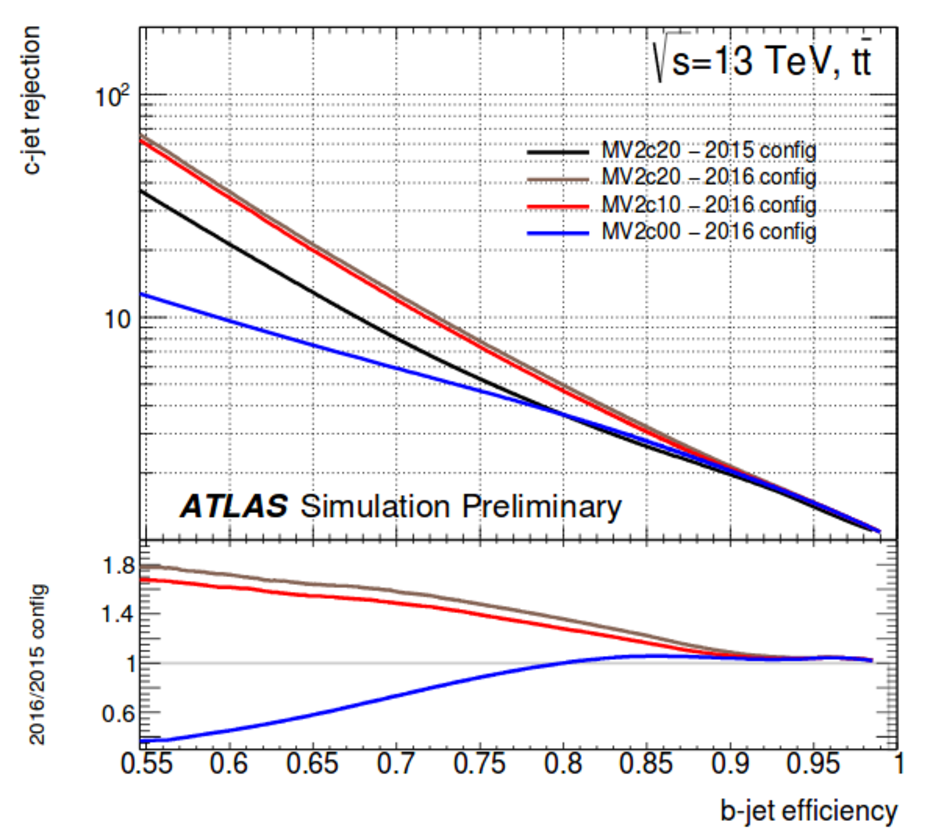
\includegraphics[width=1\textwidth]{figures/cjetrejection.pdf}
   \subcaption[c-jet rejection versus b-jet efficiency for the MV2c10 tagger.]{c-jet rejection versus b-jet efficiency for the MV2c10 tagger (red) in comparison to previous configurations evaluated on $t\bar{t}$ events. The ratio is evaluated with respect to MV2c10. \cite{MV2c10}}
   %\label{btageff}
  \end{subfigure}
 \caption[Light-flavor (a) and c-jet rejection (b) versus b-jet efficiency for the MV2c10 tagger.]{Light-flavor and c-jet rejection versus b-jet efficiency for the MV2c10 tagger. \cite{MV2c10}}
 \label{btageff}
\end{figure}
%%%%%%%%%%%%%
\section{Tau reconstruction at ATLAS}\label{taus}
Final states with tau leptons\footnote{In this section, the `term anti-tau' is absorbed in the term `tau'.}, decaying hadronically, play an important role for the physics at the {\ATLAS} experiment.  Five hadronic decay modes cover over $\SI{90}{\percent}$ of the overall hadronic modes, which results in one (1-prong) or three (3-prong) charged hadrons ($h^\pm$), up to two neutral pions ($\pi^0$) and a tau neutrino $\nu_\tau$. \cite{tauPerformance2} 
For the reconstruction of hadronic taus $\tau_\text{had-vis}$ at the {\ATLAS} detector, the anti-$k_t$ algorithm (see eq. (\ref{antiktalgorithm})) for jet formation is used (see section \ref{jets}) with a distance parameter of $R=0.4$. The requirements for the transverse momentum is $p_T>\SI{10}{\giga\electronvolt}$ and for the pseudorapidity is $|\eta|<2.5$. The hadronic identification of the tau relies on topo-clusters in the last layer of the electromagnetic calorimeter and the hadronic calorimeter. The additional track selection requires at least two associated hits in the pixel detector/IBL in the $\tau_\text{had-vis}$ direction and at least seven hits in total in the pixel detector and the SCTs. Also requirements on the distance of closest approach are set to $|d_0|<\SI{1.0}{\milli\meter}$ in the transverse plane and to $|\Delta z_0\sin\theta|<\SI{1.5}{\milli\meter}$.\cite{tauPerformance}\newline
Due to the fact that the reconstruction of tau candidates provides very little rejection against jet background a detailed set of discriminating variables\footnote{They can be found in \cite{tauPerformance}.} are introduced. Tau identification relies on separate boosted decision trees (BDT) for each prong case. The working points for that are labeled \textit{loose}, \textit{medium} and \textit{tight} corresponding to different signal efficiency values. In case of 1-prong they are, respectively, $0.6$, $0.55$ and $0.45$ for loose, medium and tight. The working points for 3-prong decays correspond to $0.5$, $0.4$, $0.3$. \cite{tauPerformance}\newline
To ensure that electrons will be not misinterpreted as 1-prong tau decays an additional BDT is implemented as a tau-electron veto. It has the same classification of \textit{loose}, \textit{medium} and \textit{tight}, but with signal efficiencies of $0.95$, $0.85$ and $0.75$ respectively. \cite{elBDT}
%
%
\section{Monte Carlo simulations}\label{MCsim}
A steady comparison and adaption of theory and experiment is crucial to be able to draw physically reliable conclusions. This fact holds true for high energy particle collision experiments, like the {\LHC}. Therefore predictions for collision events, the creation of new particles, the understanding of decays and fragmentation of these generated particles, modeling the underlying event, predictions to the subsequent hadronisation of quarks, the calculation of interactions with the detector and predictions of final states are necessary for the search of new physics. These scenarios are an extremely challenging endeavor. Typically hundreds of particles of different kinds are involved and their energy and momentum spectra are widely distributed over different orders of magnitude. One important cornerstone to cope with the above mentioned challenges are Monte Carlo (MC) simulations. \cite{bigMC}\par
MC simulations are based on an algorithm relying on sequences of pseudo random numbers. Effectively it is a method to numerically compute multidimensional integrals over a complex region as it is often the case for matrix elements in perturbation theory. \cite{MCbook} The MC chain for the {\ATLAS} detector consists of three main steps. This includes the generation of MC events with event generators and the subsequent simulation of fragmentation and showering processes in the first step. The second step is the simulation of the detector and the propagation of the particles through it with the associated interactions and, as third step, the digitization of energy deposits in the detector's sensitive areas. This digitization step involves the simulation of the resulting signals in the readout system for comparison with real data. The detailed implemented simulation of the detector and the particles interaction with it is done with {\GEANT}4\cite{GEANT4}, which additionally considers realistic detector conditions and misalignments as well as the detector response to be as realistic as possible. This fact enhances the digital copy to furthermore test the effectiveness of proposed search strategies for specific signatures like the ones created from exotic particles. \cite{ATLASSim}
%aus Verenas MA: ATLAS detector and physics performance: Technical design report, 2 1999. CERN-LHCC-99-015
%%%%%%%%%%%%%%%%%%%%%%%%%%%%%%%%%%%%%%%%%%%%%%%%%%%%%%%%%%%%%%%%%%%%%%%%%%%%%%%%%%%%%%%%%%%%%%%%%%%%%%%%%%%%%%%%%%
\chapter{Analysis}\label{analysis}
Before investigating the research question formulated in section \ref{startingpoint}, the framework principles have to be defined. The MC samples and data samples, which are taken into account, are listed in detail in section \ref{MCsamples}. The physical object definition and the event selection for the performed analysis are presented in section \ref{physObj} and \ref{eventselection}.  
%das wurde zu LQ verfrachtet, siehe LQ Kapitel: besserer Zusammenhang
%\section{Current status in the search for scalar leptoquarks}
%\section{Starting point and research question for the analysis}
\section{Datasets and Monte Carlo samples}\label{MCsamples}
%%%%%%%%%%%%%%%%%%%%%%%%%%%%%%%%%%%%%%%%%%%%%%%%%%%%%%%%%%%%%%%%%%%%%%%%%%%%%%%%%%%%%%%%%%%%%%%%%%%%%%%%%%%%%%%%%%%
The motivation is to estimate tau efficiencies for the search for third generation leptoquarks in the $t\tau^{-}+\bar{t}\tau^{+}$ channel. To draw convincing conclusions from the efficiency study, a good estimation of the standard model background events has to be chosen. The choice of background samples involves the following considerations:\newline
%ttbar teil
Dominant background processes, contaminating the potential LQ signal, originate from QCD events producing top-quark pairs and top-pair production in association with Higgs, where Higgs decays into tau leptons.\newline
The differential cross section for top-quark pair generation at $\sqrt{s}=\SI{13}{\tera\electronvolt}$ is \SI{829\pm189}{\pico\barn} \cite{ttbarpairproduction} including the statistical and the systematic uncertainty as well as the uncertainty from the luminosity measurement. Due to the nature of a proton-proton collider mainly gluon fusion ($\SI{90}{\percent}$ \cite{PhysRevD}) is responsible for the top-quark pair production at the {\LHC}. Also quark fusion can lead to $t\bar{t}$ states. The corresponding Feynman diagrams involved in the pair production are shown in figure \ref{ttbarproduction}. Because of its high production cross section and the lack of naturally existing taus, the $t\bar{t}$ sample is the ideal candidate to study jets and especially b-jets that fake as a hadronic tau.  
%
\begin{figure}
 \centering
  \begin{subfigure}[t]{0.49\textwidth}
   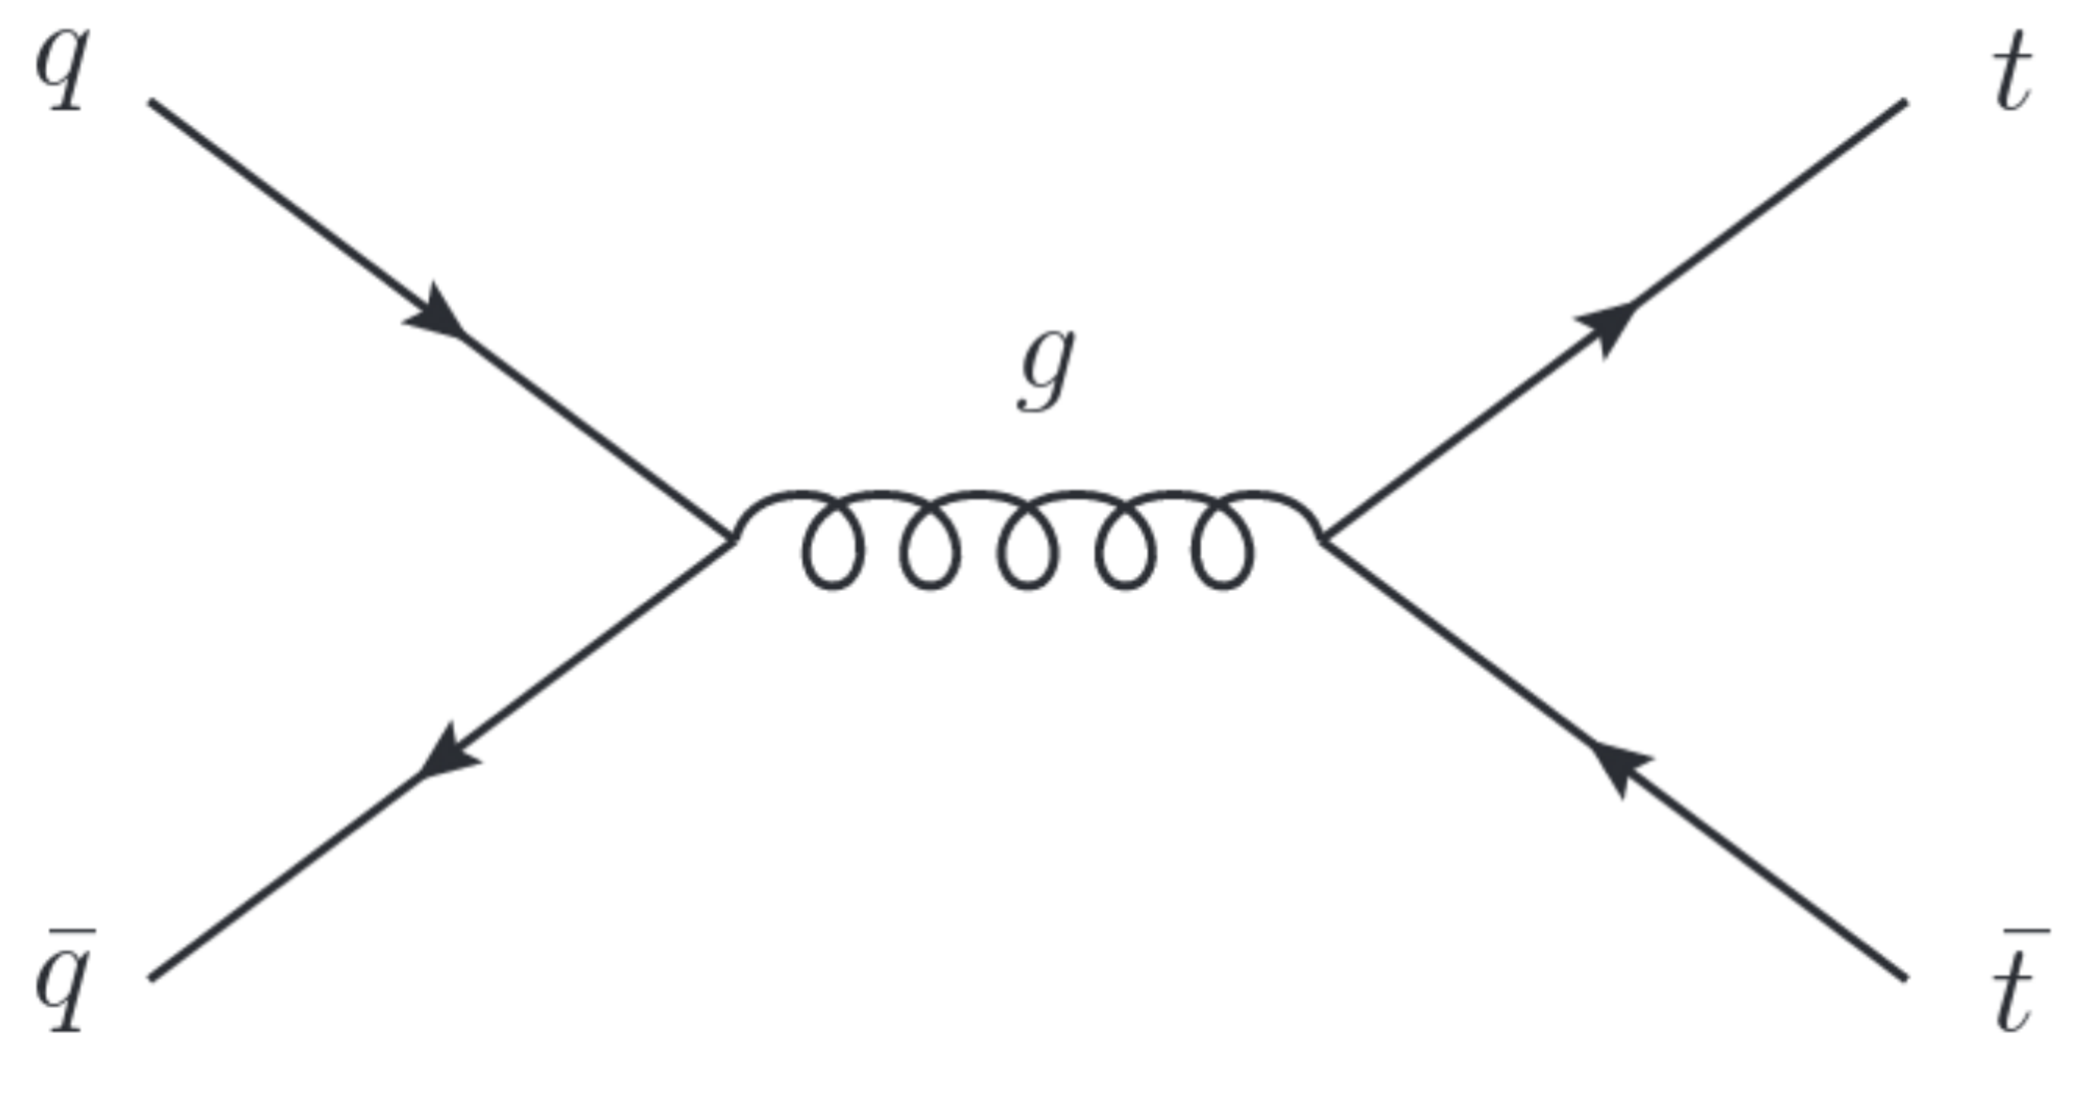
\includegraphics[width=\textwidth]{figures/ttbara.pdf}
    \subcaption[Quark fusion process generating a top-quark pair in the s-channel.]{Quark fusion process generating a top-quark pair in the s-channel \cite{Feynmanttbar}.}
   %\label{ATLASDesign}
  \end{subfigure}
  \begin{subfigure}[t]{0.49\textwidth}
   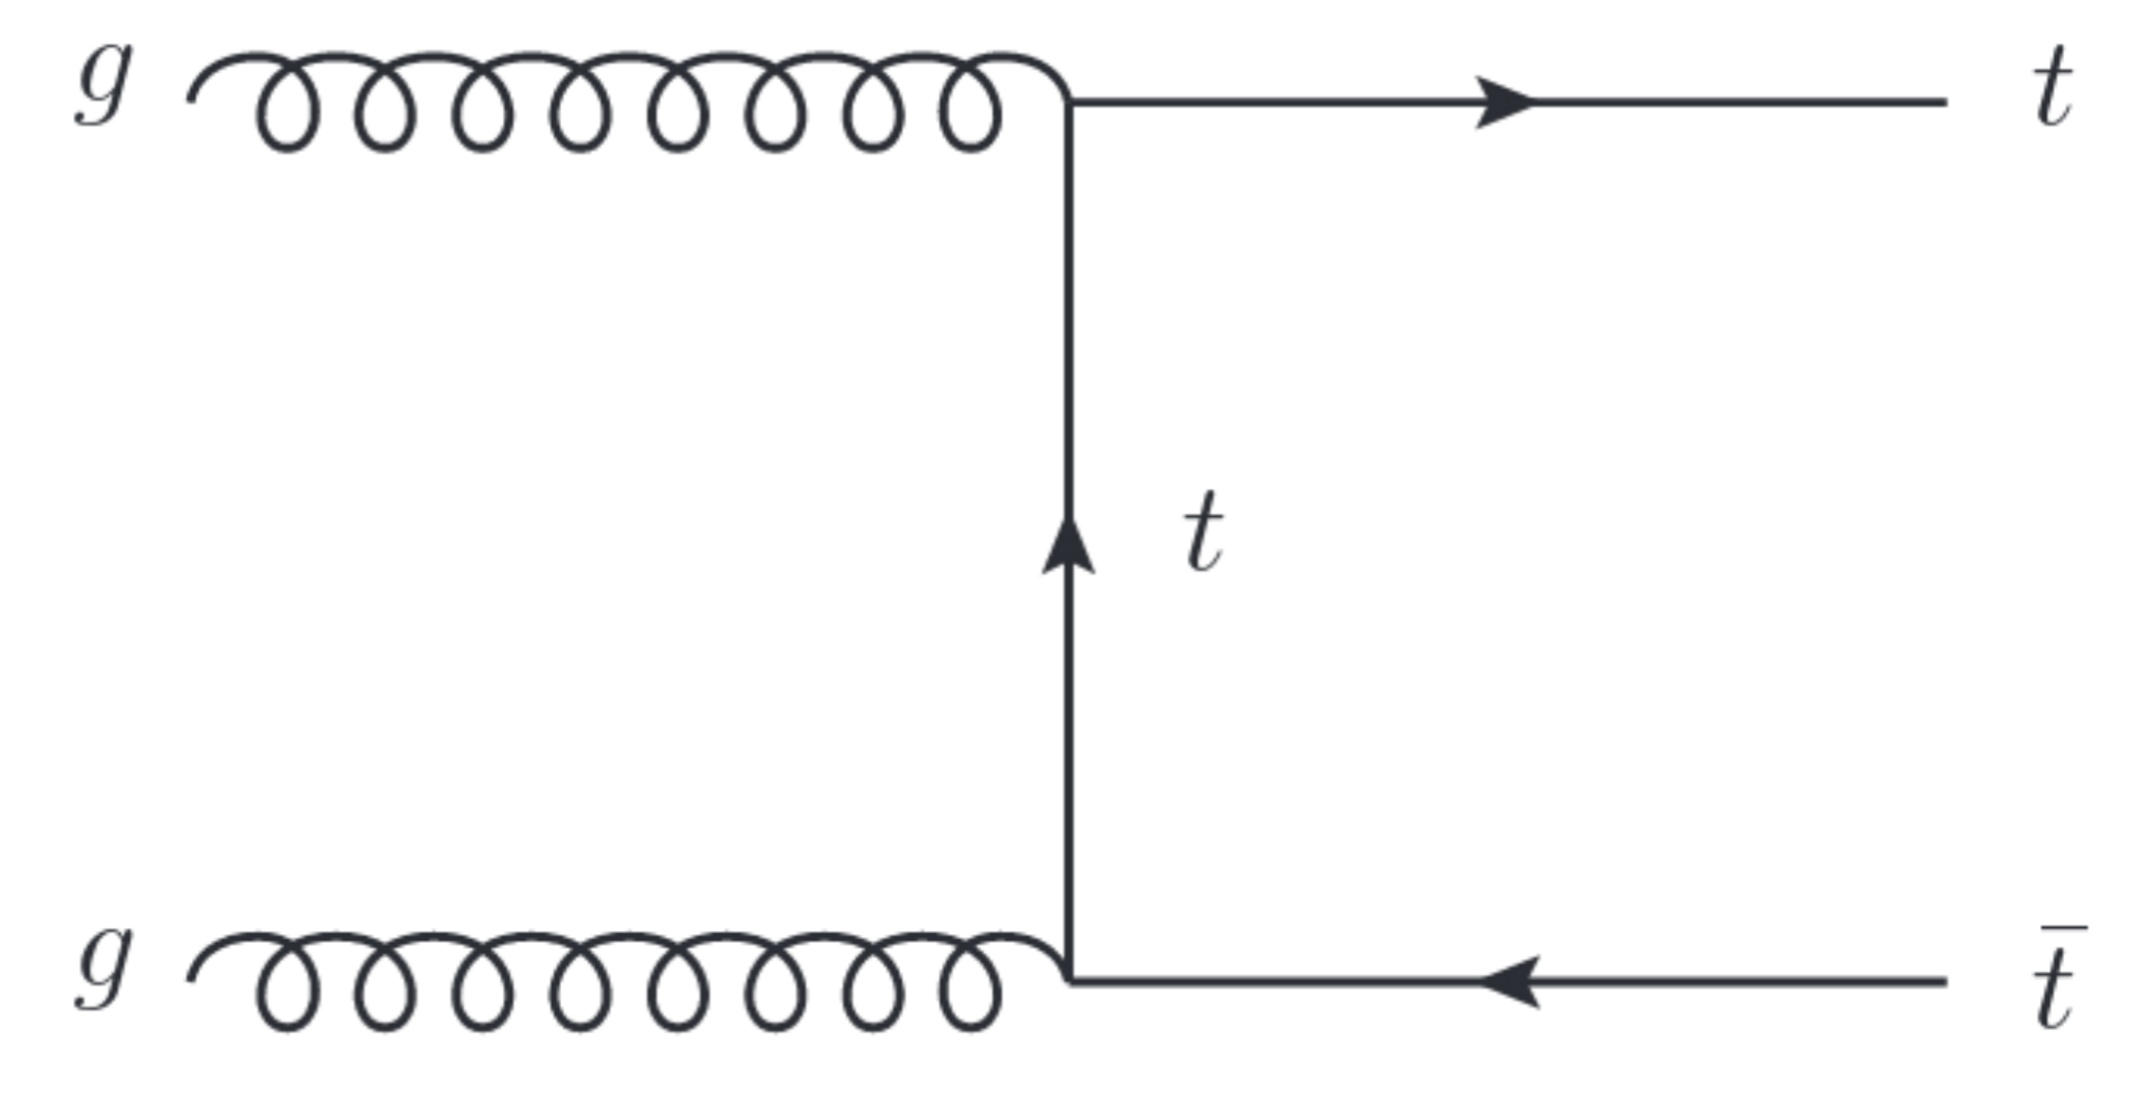
\includegraphics[width=\textwidth]{figures/ttbarb.pdf}
   \subcaption[Gluon fusion process generating a top-quark pair in the t-channel.]{Gluon fusion process generating a top-quark pair in the t-channel \cite{Feynmanttbar}.}
   %\label{btageff}
  \end{subfigure}
 \begin{subfigure}[t]{0.49\textwidth}
   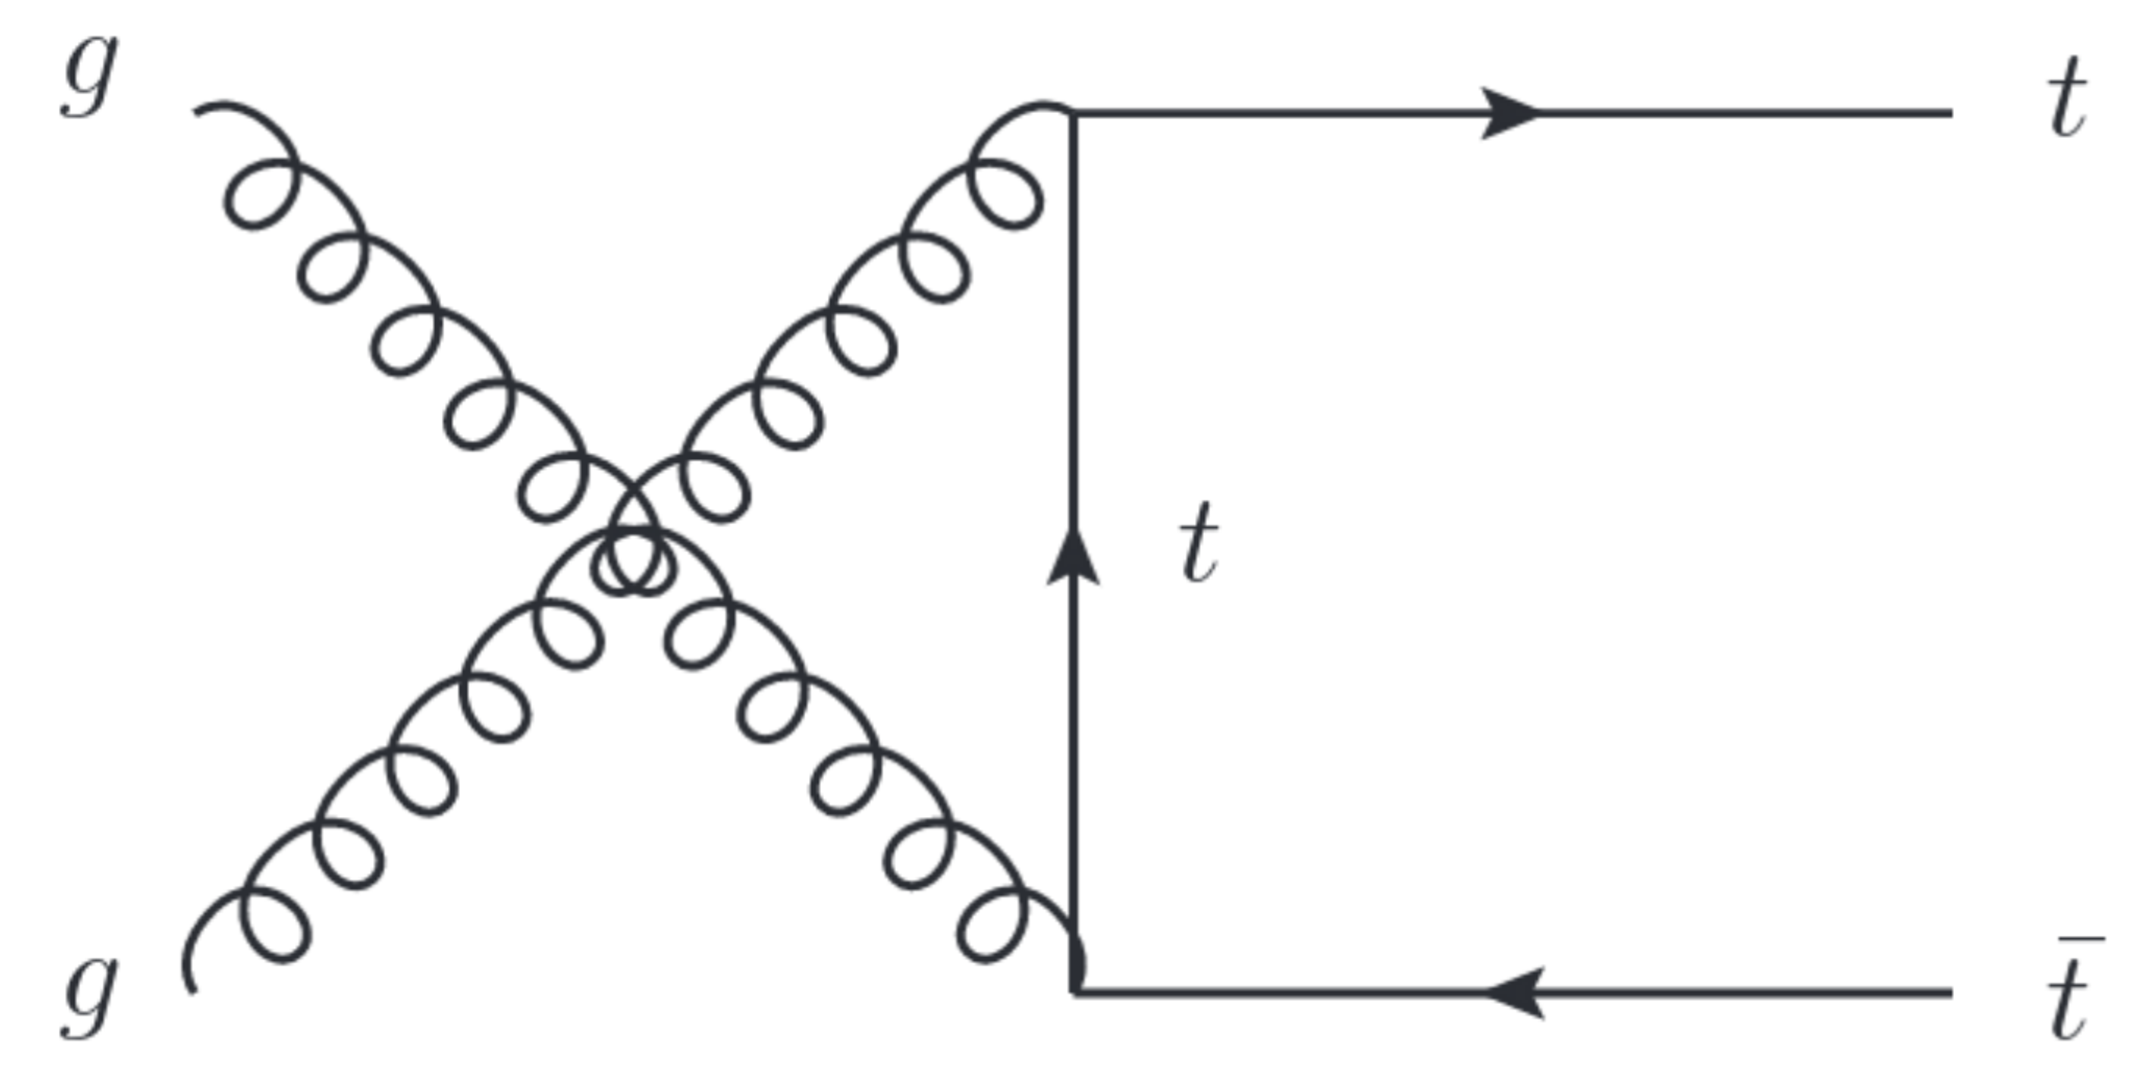
\includegraphics[width=\textwidth]{figures/ttbarc.pdf}
    \subcaption[Gluon fusion process generating a top-quark pair in the u-channel.]{Gluon fusion process generating a top-quark pair in the u-channel \cite{Feynmanttbar}.}
   %\label{ATLASDesign}
  \end{subfigure}
  \begin{subfigure}[t]{0.49\textwidth}
   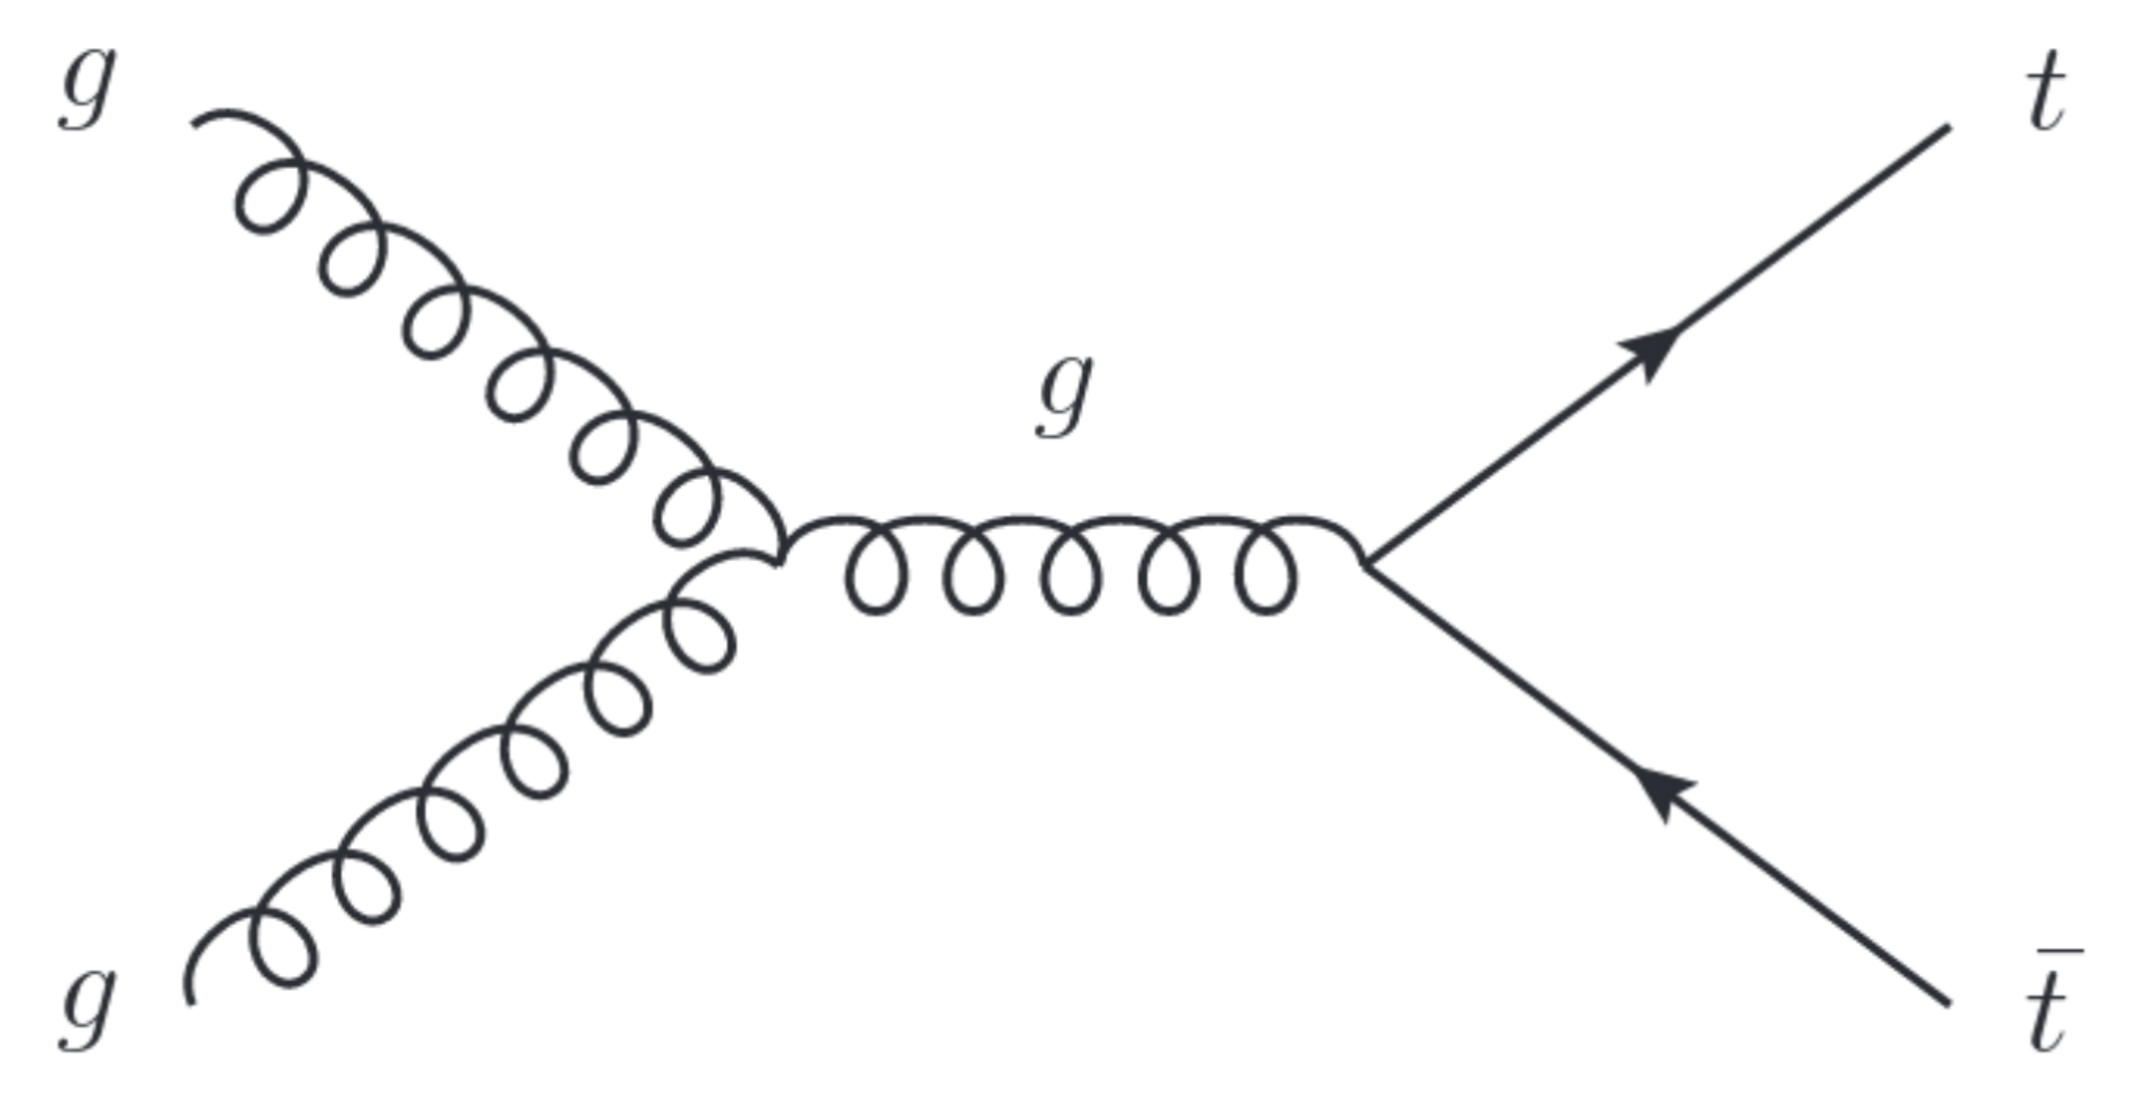
\includegraphics[width=\textwidth]{figures/ttbard.pdf}
    \subcaption[Gluon fusion process generating a top-quark pair in the s-channel.]{Gluon fusion process generating a top-quark pair in the s-channel \cite{Feynmanttbar}.}
   %\label{ATLASDesign}
  \end{subfigure}
 \caption[Feynman diagrams showing the dominant top-pair production at the {\LHC}.]{Feynman diagrams showing the dominant top-pair production at the {\LHC} including quark fusion (a) and gluon fusion (b)-(d) \cite{Feynmanttbar}.}
 \label{ttbarproduction}
\end{figure}
%
%dann noch H teil.
The total cross section measured for Higgs production is $\left( 12^{+25}_{-16} \right)\,\text{pb}$ \cite{HiggsCrossSection}. The dominant Higgs production mechanisms of leading order at hadron colliders are gluon fusion, vector boson fusion, Higgs-strahlung or the associated production with a pair of top (bottom) quarks \cite{PhysRevD}. The relevant background SM process for the search of LQs is the associated Higgs production with a top pair, which can mimic the $t\tau^{-}+\bar{t}\tau^{+}$ state. The $t\bar{t}H$ cross section is $\SI{0.51\pm0.06}{\pico\barn}$. The corresponding Feynman diagram for $t\bar{t}H$ production is depicted in figure \ref{ttHproduction}. The used $t\bar{t}H$ sample (cf. section \ref{MCsamples}) acts as an inclusive sample, which allows all possible Higgs decays. The Higgs coupling strength is proportional to the particle's mass and therefore the direct decay of the Higgs boson into a tau-pair is possible, as it involves the heaviest lepton (cf. \ref{SMtable}). Together with the decay $H\rightarrow b\bar{b}$ the mode $H\rightarrow \tau^-\tau^+$ is the dominant process below the threshold of $\SI{160.8}{\giga\electronvolt}$ and $\SI{182.4}{\giga\electronvolt}$ that is the on-shell $\text{H}^0\rightarrow\text{W}^-\text{W}^+$ and $\text{H}^0\rightarrow\text{Z}^0\text{Z}^0$ production \cite{PhysRevD}. On-shell means that both vector bosons are produced with their likeliest mass rather than producing one vector boson of the pair as a virtual particle. From the point of view of the Higgs boson's coupling to large masses in principle $H\rightarrow t\bar{t}$ is also a possible decay mode. But the di-top mass exceeds the Higgs mass by a factor of roughly three times, which suppresses that decay due to the fact that the top-pair can exist only virtually.    
%
\begin{figure}[htbp]                                 
 \begin{center}                                       
  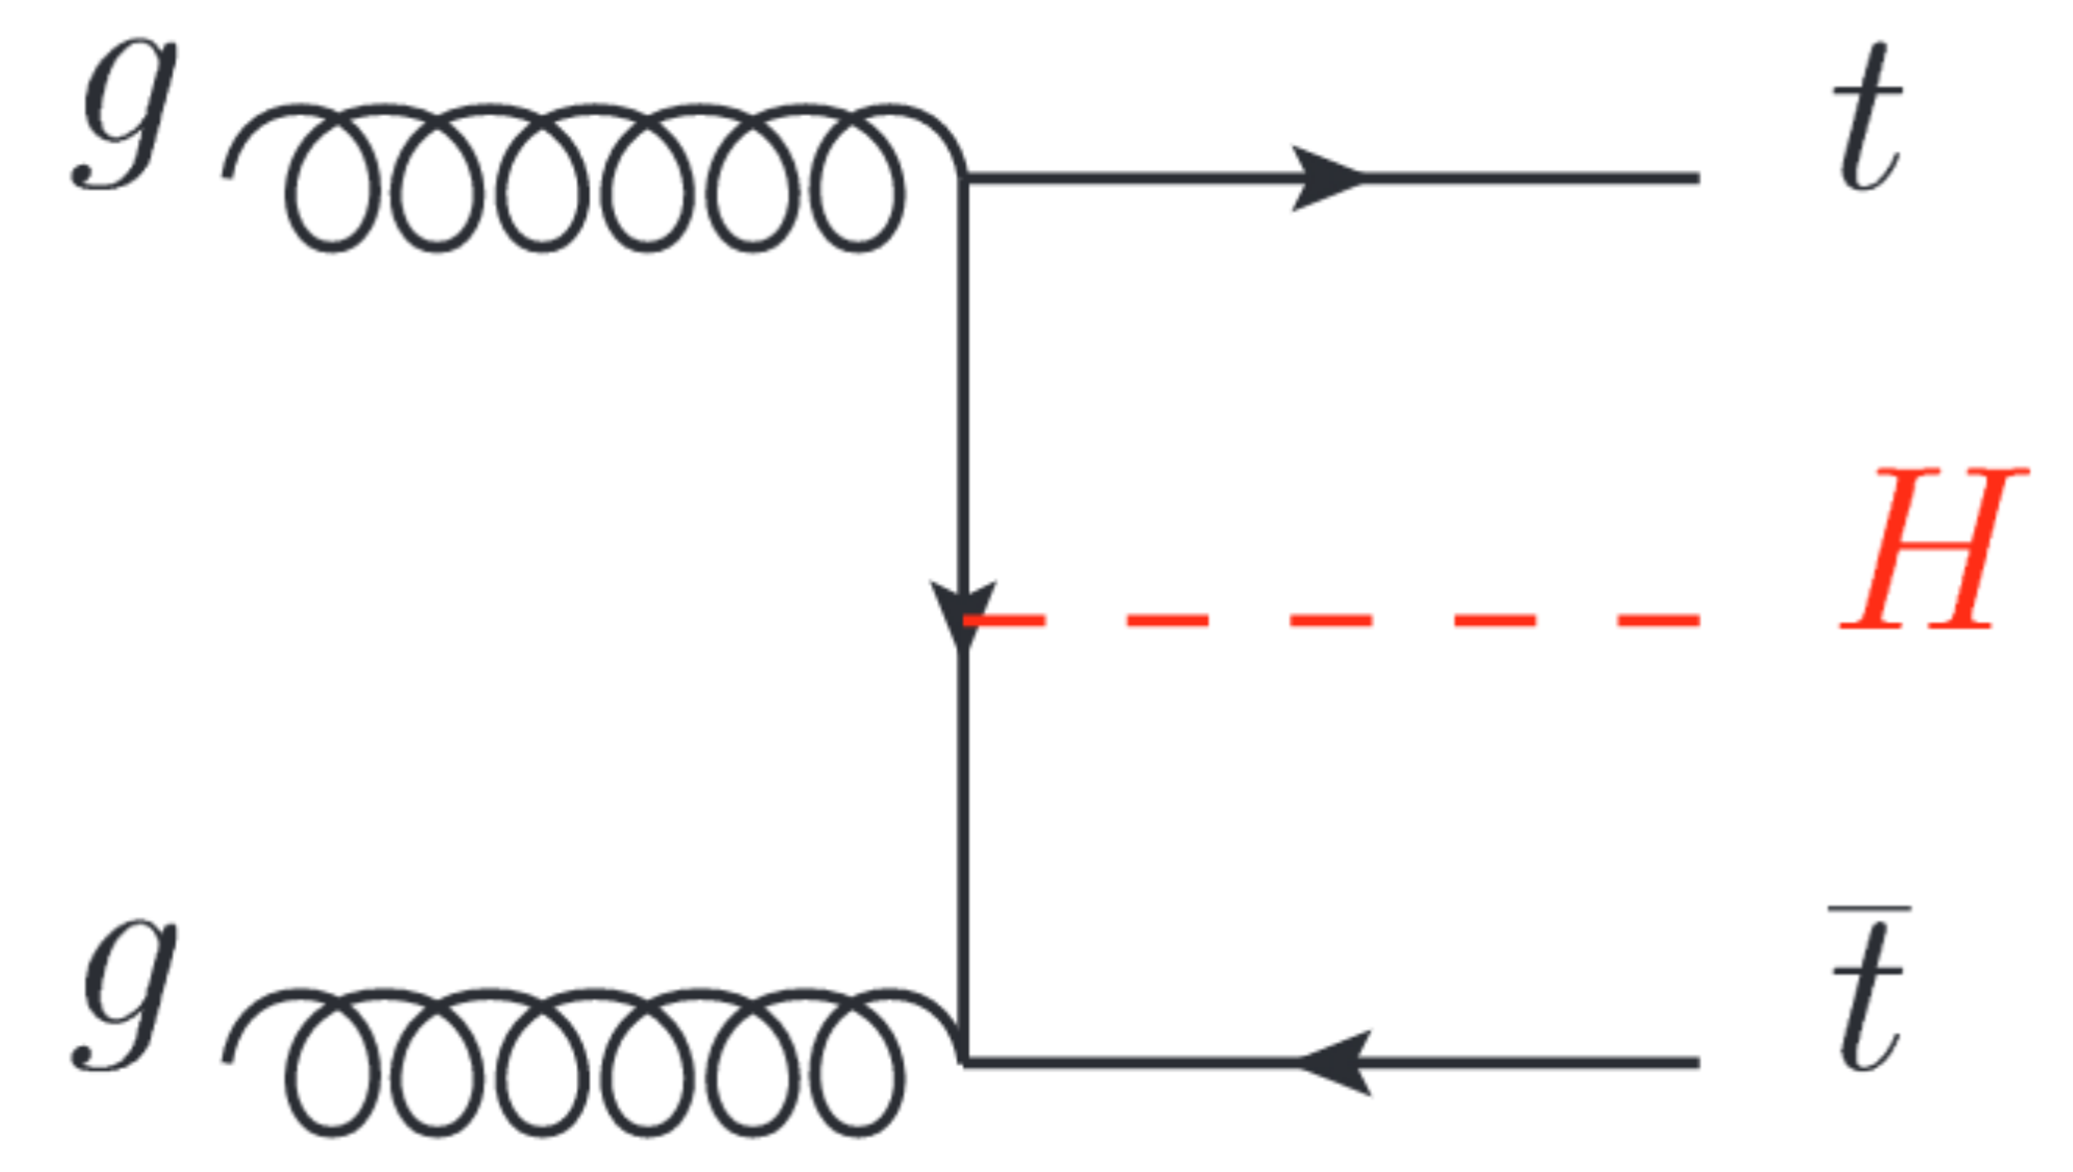
\includegraphics[width=0.3\linewidth]{figures/ttHproduction.pdf} 
   \caption[Higgs production associated with a top-quark pair.]{Feynman diagram in leading order for the top-quark pair associated Higgs production \cite{PhysRevD}.}
  \label{ttHproduction}                                    
 \end{center}
\end{figure}
%
The above mentioned aspects make the $t\bar{t}H$ sample a good candidate to study faked taus from jets with the additional condition that also real taus are naturally present compared to the top-pair production. Furthermore efficiencies for different tau selections can be studied as well in this events as they occur as signal signatures. Findings in the background processes then can be compared to the LQ signal samples (see section \ref{signaleff}). \newline
Together these to background samples cover most of the contamination of the $t\tau^{-}+\bar{t}\tau^{+}$ for the LQ search.\par
The MC samples in the analysis are used to investigate the signal and background composition and to estimate fake rates related to tau reconstruction of LQs in the $t\tau^{-}+\bar{t}\tau^{+}$ channel. The analysis uses two types of MC samples. One category includes the LQ signal following the decays after the mBRW model (cf. section \ref{effmodels}). These signal samples were produced with the event generator {\aMCNLO} (v2.6.0) \cite{aMCNlo} with two different mass points of the LQ of $m_{LQ}=\SI{500}{\giga\electronvolt}$ and $m_{LQ}=\SI{1}{\tera\electronvolt}$ and with a production cross section of $\SI{271}{\femto\barn}$ $\SI{3}{\femto\barn}$ respectively. The top pair is allowed to decay either fully leptonically or semi-leptonically in the LQ sample (cf. section \ref{startingpoint}). The parton showering and fragmentation as well as the underlying event generation were done with {\Pythia} \cite{Pythia8} with the particle distribution function (PDF) sets {\NNPDFd} \cite{NNPDF} and the A14 \cite{A14} tunes at next-to-leading order (NLO) in matrix calculation. \newline         
The other category of simulations includes main background contributions of standard model processes as motivated above. That is background from $t\bar{t}$ pairs and inclusive $t\bar{t}H$ decay processes. The $t\bar{t}$ samples are generated with {\POWHEG} \cite{Powheg} and allow the $t\bar{t}$ pair to decay fully leptonically. Showering, fragmentation and the underlying event generation are simulated with the generator {\Pythia} at NLO with the PDF set of {\NNPDFz} and the parameter set of A14. The $h_\text{damp}$ parameter was set to $\SI{258.75}{\giga\electronvolt}$, which is a resummation damping factor and regulates the highest transverse momentum of the first additional parton radiation beyond the Born level \cite{hdamp}\cite{hdamp2}.\newline
%
\begin{table}[htbp]
		\centering
                \renewcommand{\arraystretch}{1.2}       
		\begin{tabular*}{\linewidth}{@{\extracolsep{\fill}}cc}
		\hline
		\hline
		\textbf{data-taking year}&  \textbf{integrated luminosity}
		\\
		\hline
                $2018$                & $\SI{60}{\per\femto\barn}$
                \\
                $2017$                & $\SI{44}{\per\femto\barn}$
                \\
                $2016$                & $\SI{33}{\per\femto\barn}$
                \\
                $2015$                & $\SI{3}{\per\femto\barn}$
                \\
                \hline
                \textbf{total}        & $\SI{140}{\per\femto\barn}$
                \\
		\hline
		\hline
		\end{tabular*}
		\caption[Integrated luminosity for the data-taking periods 2015-2018.]{Integrated luminosity for the data-taking periods 2015, 2016, 2017 and 2018.}
\label{datalumi}
\renewcommand{\arraystretch}{1}
\end{table}
%
The $t\bar{t}H$ sample is generated with {\POWHEG}. Like for the $t\bar{t}$ samples, the event generator {\Pythia} at NLO with the PDF set of {\NNPDFz} and the parameter set of A14 was used to simulate the showering, fragmentation and underlying event. The mass of the Higgs boson is set to $\SI{125}{\giga\electronvolt}$ and the resummation parameter was set to $\SI{325.5}{\giga\electronvolt}$. \newline
For all samples the {\EvtGen} (v1.6.0) \cite{EvtGen} program was used for the decay of the bottom and charm hadrons produced by the top-quark decay.\newline
Data sets of the data-taking periods 2015, 2016, 2017 and 2018, which were produced at a center of mass energy of $\sqrt{s}=\SI{13}{\tera\electronvolt}$, are studied and compared to the MC predictions. Table \ref{datalumi} shows the integrated luminosity of the different years and the total integrated luminosity of $\SI{140}{\per\femto\barn}$ used in the analysis. Because of the fact that for this study no systematic uncertainties are considered, the luminosity values are rounded to the next whole number. Their uncertainty contributions of usually few percent are small compared to uncertainties from systematics.
%%%%%%%%%%%%%%%%%%%%%%%%%%%%%%%%%%%%%%%%%%%%%%%%%%%%%%%%%%%%%%%%%%%%%%%%%%%%%%%%%%%%%%%%%%%%%%%%%%%%%%%%%%%%%$
\section{Physical object selection}\label{physObj}
The physical object selection for electrons, muons, hadronic taus, jets and b-jets in the analysis is described in this section. For the general reconstruction concepts of physical objects see chapter \ref{detectorsignatures}.\par
The {\ATLAS} software framework for event generation, simulation, reconstruction and derivation production (cf. also section \ref{MCsim}) is Athena \cite{Athena}. %The management and build of the software packages rely on CMake.
The standard package for physical object reconstruction used in this analysis is AnalysisTop. It is derived from the general software chain of AthAnalysisBase specifically adapted for the needs of the top-quark analysis group. The \texttt{C++} framwork {\ROOT} is used as data analysis tool. For this work a package based on AnalysisTop of release 21.2.56 (build on November 29, 2018) was used.\par
\subsubsection*{Electrons}
Electrons have to fulfill the tight quality requirement and need to have at least a transverse momentum of $p_T>\SI{27}{\giga\electronvolt}$ and lie within the pseudorapidity range of $|\eta|<2.5$. In order to get a clean signal from a leptonic decaying top quark, the electrons have to meet the $p_T$ dependent isolation requirements. For the electron trigger requirements see the paragraph `Lepton trigger' below.
\subsubsection*{Muons}
Muons have to meet the medium quality requirement and need to have a transverse momentum of $p_T>\SI{27}{\giga\electronvolt}$. The selected muons are reconstructed as a combined muon within a pseudorapidity region of $|\eta|<2.5$. Analogous to the electron selection for a clean lepton signal, the muon has to further fulfill the $p_T$ dependent isolation requirements. For the muon trigger requirements see the paragraph `Lepton trigger' below. 
\subsubsection*{Taus}
Taus selected for this analysis need to have a transverse momentum of at least $p_T>\SI{25}{\giga\electronvolt}$ and must lie within the pseudorapidity range of $|\eta|<2.5$. Additional to that the taus have to decay hadronically. Following their basic reconstruction procedure, taus have to meet the conditions of the loose working point (see section \ref{taus}). To avoid misinterpretations of electrons as taus, the corresponding working point is set to loose.
\subsubsection*{Jets}
Jets are reconstructed with the anti-$k_T$ algorithm and need to have a transverse momentum of at least $p_T>\SI{25}{\giga\electronvolt}$. 
\subsubsection*{b-jets}\label{physObj:bjet}
For the b-jet selection the b-tagger MV2c10 is used with a working point of $\SI{77}{\percent}$ b-tagging efficiency.
\subsubsection*{Lepton trigger}\label{leptontrigger}
The trigger requirements relevant for the analysis on electrons and muons are described here and are categorized each after the corresponding data-taking period.\par
Electrons are required to to pass the `OR' condition of the single electron triggers. This means that for an electron at least one of the triggers presented in table \ref{etriggersTable} had indicated an electron signature for the specific data-taking period in the detector.\par
%
\begin{table}[htbp]
		\centering
                \footnotesize
                \renewcommand{\arraystretch}{1.2}       
		\begin{tabular*}{\linewidth}{@{\extracolsep{\fill}}ccc}
		\hline
		\hline
		\textbf{data-taking year}&  \textbf{`OR' required trigger} & \textbf{important parameter}
		\\
                \hline
                \multirow{3}{*}{$2018$, $2017$, $2016$}                & \texttt{e26\textunderscore lhtight\textunderscore nod0\textunderscore ivarloose}   & $p_T>\SI{26}{\giga\electronvolt}$, tight working point 
                \\
                & or \texttt{e60\textunderscore lhmedium\textunderscore nod0}   & $p_T>\SI{60}{\giga\electronvolt}$, medium working point 
                \\
                & or \texttt{e140\textunderscore lhloose\textunderscore nod0}       & $p_T>\SI{140}{\giga\electronvolt}$, loose working point 
                \\
                \hline
                \multirow{3}{*}{$2015$}                & \texttt{e24\textunderscore lhmedium\textunderscore L1EM20VH}   &      $p_T>\SI{24}{\giga\electronvolt}$, medium working point 
                \\
                & or \texttt{e60\textunderscore lhmedium}       & $p_T>\SI{60}{\giga\electronvolt}$, medium working point
                \\
                & or \texttt{e120\textunderscore lhloose}       & $p_T>\SI{120}{\giga\electronvolt}$, loose working point
                \\
		\hline
		\hline
		\end{tabular*}
		\caption[List of single electron triggers.]{List of single electron triggers.}
\label{etriggersTable}
\renewcommand{\arraystretch}{1}
\end{table}
%
The same strategy as it is used for electrons is valid for muons. Muons are required to to pass the `OR' condition of the single muon triggers. This means that for an muon at least one of the triggers presented in table \ref{mutriggersTable} had indicated a muon signature for the specific data-taking period in the detector.\par
%
\begin{table}[htbp]
		\centering
                \footnotesize
                \renewcommand{\arraystretch}{1.2}       
		\begin{tabular*}{\linewidth}{@{\extracolsep{\fill}}ccc}
		\hline
		\hline
		\textbf{data-taking year}&  \textbf{`OR' required trigger} & \textbf{important parameter}
		\\
                \hline
                \multirow{2}{*}{$2018$, $2017$, $2016$}                & \texttt{mu26\textunderscore ivarmedium} & $p_T>\SI{26}{\giga\electronvolt}$, medium working point
                \\
                & or \texttt{mu50}      & $p_T>\SI{50}{\giga\electronvolt}$
                \\
                \hline
                $2015$                & \texttt{mu20\textunderscore iloose\textunderscore L1MU15} & $p_T>\SI{26}{\giga\electronvolt}$, loose working point
                \\
		\hline
		\hline
		\end{tabular*}
		\caption[List of single muon triggers.]{List of single muon triggers.}
\label{mutriggersTable}
\renewcommand{\arraystretch}{1}
\end{table}
%
For more detailed information about the trigger requirements and their exlanation see section \ref{eReconstruction} and \ref{muReconstruction}.
\subsubsection*{Overlap removal}\label{overlapremoval}
To avoid misinterpretations an overlap removal between different objects acts like a veto and is applied for the event reconstruction. The overlap is determined by thresholds in the separtion variable $\Delta R=\sqrt{\Delta\eta^2+\Delta\phi^2}$. The following overlap removals are applied for objects like electrons $e$, muons $\mu$, tau leptons $\tau$ and jets $j$:
\begin{itemize}
\item electron removal if $\Delta R(e,j)<0.4$
\item muon removal if $\Delta R(\mu,j)<0.4$
\item jet removal if $\Delta R(j,e)<0.2$
\item tau removal if $\Delta R(\tau,l)< 0.4$ with $l=e,\mu$
\end{itemize}
%https://indico.cern.ch/event/784955/contributions/3265310/attachments/1776237/2890543/SR_definitions.pdf
%overlap removal: default between <e,jet>, <mu,jet>, <jet,e> 0.2 nicht tau, 0.4 tau
%%%%%%%%%%%%%%%%%%%%%%%%%%%%%%%%%%%%%%%%%%%%%%%%%%%%%%%%%%%%%%%%%%%%%%%%%%%%%%%%%%%%%%%%%%%%%%%%%%%%%%%%%%%%%%
\section{Event selection}\label{eventselection}
The signal and background studies for the $t\tau^{-}+\bar{t}\tau^{+}$ channel involves the event selection shown in figure \ref{selection}.\newline
%
\begin{figure}[htbp]                                 
 \begin{center}                                       
  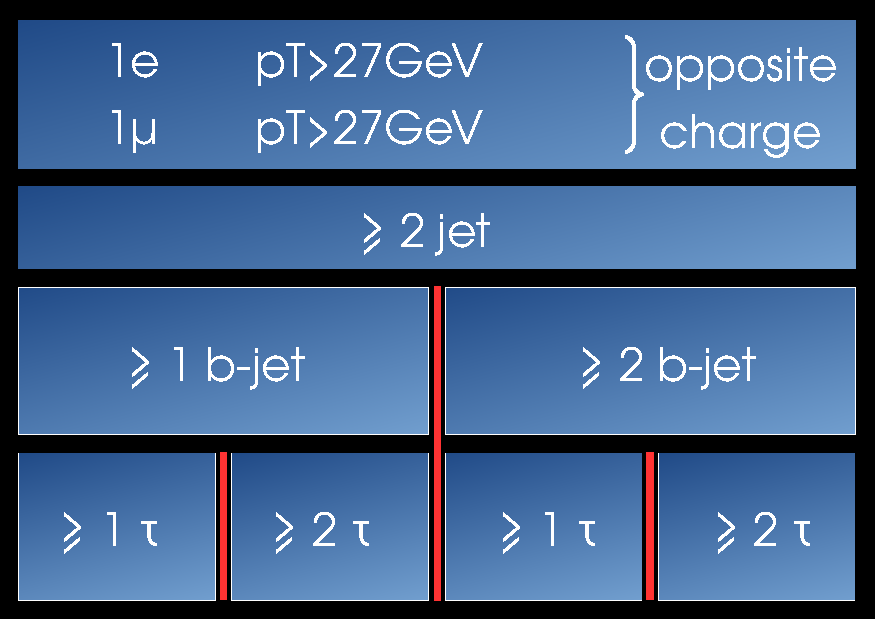
\includegraphics[width=0.45\linewidth]{figures/selection.pdf} 
   \caption[Overview of the event selection.]{Overview of the event selection involved for the signal and background studies in the $t\tau^{-}+\bar{t}\tau^{+}$ channel.}
  \label{selection}                                    
 \end{center}
\end{figure}
%
The selection includes one electron and one muon of opposite electrical charge and a transverse momentum of at least $p_T>\SI{27}{\giga\electronvolt}$. This di-lepton selection covers the leptonic decay of the top-pair mediated by the $W^-$ boson in case of the anti-top quark and mediated by the $W^+$ in case of the top quark. Due to conservation of the electric charge the resulting leptons of the subsequent decay of the $W^\pm$ boson is of opposite sign. In addition to that at least two jets are selected because the weak top-pair decay produces a bottom-pair (cf. figure \ref{topdecay}), which will result in a jet. At least two of the above selected jets have to be b-tagged or at least one of the above jets have to be b-tagged. To cover the full $t\tau^{-}+\bar{t}\tau^{+}$ channel, an additional selection is made to select at least either one or two tau leptons for each cases of b-jet selection. The samples include these categories of one b-tagged jet, two b-tagged jets, one tau or two taus and the corresponding distributions as separate categories.
%%%%%%%%%%%%%%%%%%%%%%%%%%%%%%%%%%%%%%%%%%%%%%%%%%%%%%%%%%%%%%%%%%%%%%%%%%%%%%%%%%%%%%%%%%%%%%%%%%%%%%%%%%%%%
\chapter{Results}\label{results}
%%%%%%%%%%%%%%%%%%%%%%%%%%%%%%%%%%%%%%%%%%%%%%%%%%%%%%%%%%%%%%%%%%%%%%%%%%%%%%%%%%%%%%%%%%%%%%%%%%%%%%%%%%%%%
\section{Number of event candidates}\label{eventYield}
The observed and predicted number of event candidates for the event selection described in section \ref{eventselection} is summarized in this chapter.\par
The event yield table \ref{eventYieldTable} includes all the main background contributions from $t\bar{t}$ and $t\bar{t}H$ processes as well as the LQ signal samples generated with two different mass points compared to the number of event candidates from data. The error consists of the statistical uncertainty only. The differentiation of the event number categories follow the event selection described in section \ref{eventselection}. Its main categories include the selection of either at least one b-jet or at least two b-jets. The decay channel of the LQ involves a pair of b-quarks originating from the subsequent top-pair decay mediated by the weak interaction (cf. section \ref{startingpoint}). After the two b-jet selection the sample is dominated by contributions from standard model $t\bar{t}$ productions. Selecting only one b-jet will be useful for a full search strategy for scalar LQs. Due to the leptoquarks' high masses of $\SI{500}{\giga\electronvolt}$ and $\SI{1}{\tera\electronvolt}$ and experimental exclusion limits as well as theoretically considerations, the assumed production cross section at the {\LHC} is small compared to abundant QCD processes of the SM\footnote{For a cross section comparison see \ref{MCsamples}, where the different samples are discussed.}. Thus the looser selection of at least one b-jet and the resulting higher event yield gives room for tighter cuts on kinematic variables to optimize the signal and at the same time looses almost nothing in background rejection. \newline
%
\begin{sidewaystable}[htbp]
		\centering
                \renewcommand{\arraystretch}{1.5}       
		\begin{tabular*}{\linewidth}{@{\extracolsep{\fill}}ccccccc}
		\hline
		\hline
		\textbf{channel} &      \multicolumn{6}{c}{\textbf{event selection}}
		\\
                & $\geq 1\,$b-jet &     $\geq 1\,$b-jet $+$ $\geq 1\tau$ &   $\geq 1\,$b-jet $+$ $\geq 2\tau$ &     $\geq 2\,$b-jet &     $\geq 2\,$b-jet $+$ $\geq 1\tau$ &     $\geq 2\,$b-jet $+$ $\geq 2\tau$ 
		\\
		\hline
                $t\bar{t}$ &    $\SI{555369\pm 303}{}$ &        $\SI{2793\pm 21}{}$ &    $\SI{7.5\pm 1.1}{}$ & $\SI{270799\pm 210}{}$ &        $\SI{765\pm 11}{}$ &   $\SI{2.99\pm 0.69}{}$
                \\
                $t\bar{t}H$ &    $\SI{517.4\pm 2.7}{}$ &        $\SI{28.02\pm 0.55}{}$ &    $\SI{1.554\pm 0.070}{}$ & $\SI{338.1\pm 1.6}{}$ &        $\SI{14.24\pm 0.37}{}$ &   $\SI{0.735\pm 0.043}{}$
                \\
                \hline
                \textbf{total} &    $\SI{555886\pm 303}{}$ &        $\SI{2821\pm 21}{}$ &    $\SI{9.0\pm 1.1}{}$ & $\SI{271137\pm 210}{}$ &        $\SI{779\pm 11}{}$ &   $\SI{3.72\pm 0.69}{}$
                \\
                \hline
                $LQ_\text{$500\,$GeV}$ &    $\SI{1304\pm 40}{}$ &        $\SI{598\pm 27}{}$ &    $\SI{96\pm 10}{}$ & $\SI{650\pm 28}{}$ &        $\SI{287\pm 19}{}$ &   $\SI{45.9\pm 6.7}{}$
                \\
                $LQ_\text{$1\,$TeV}$ &    $\SI{14.69\pm 0.41}{}$ &        $\SI{6.65\pm 0.27}{}$ &    $\SI{0.745\pm 0.093}{}$ & $\SI{7.44\pm 0.29}{}$ &        $\SI{3.38\pm 0.19}{}$ &   $\SI{0.371\pm 0.063}{}$
                \\
                \hline
                data &    $\SI{554745\pm 745}{}$ &        $\SI{3342\pm 58}{}$ &    $\SI{12.0\pm 3.5}{}$ & $\SI{265437\pm 515}{}$ &        $\SI{1022\pm 32}{}$ &   $\SI{3.0\pm 1.7}{}$
                \\
		\hline
		\hline
		\end{tabular*}
		\caption[Observed and predicted event yield for the event selection.]{The observed and predicted number of event candidates with statistical uncertainty for the event selection described in section \ref{eventselection} including the LQ signal, the background contributions of $t\bar{t}$ and $t\bar{t}H$ processes and data. The integrated luminosity is $\SI{140}{\per\femto\barn}$.}
\label{eventYieldTable}
\renewcommand{\arraystretch}{1}
\end{sidewaystable}
%
The additional selection of at least either one or at least two tau leptons impose an additional reduction on the event yield for both b-jet selections. The difference between the background simulations is that selecting $\geq 1\,\text{b-jet}+\geq 1\,\tau$ additionally results in a strong reduction of the events without any tau lepton selection down to $\SI{0.5\pm 0.75}{\percent}$ in case of the $t\bar{t}$ sample, whereas the amount in case of the $t\bar{t}H$ sample is reduced to $\SI{5.4\pm 2.0}{\percent}$. The expectation is that the events surviving the tau selection contributed from the $t\bar{t}$ sample are mainly due to faked taus. No real $\tau$ lepton is expected here. In contrast, some real $\tau$ contributions from the Higgs sample are expected from the possible decay $H^0\rightarrow \tau^-\tau^+$. This is because the Higgs coupling strength is proportional to the mass and therefore the heaviest lepton (cf. table \ref{SMtable}) is a direct decay product of the Higgs boson. The reduction of the event yield for both signal samples, when at least one tau is selected, is only down to $\SI{45.9\pm 5.5}{\percent}$ (mass point \SI{500}{\giga\electronvolt}) and $\SI{45.3\pm 4.9}{\percent}$ (mass point $\SI{1}{\tera\electronvolt}$). The data event candidates reduce to $\SI{0.6\pm1.7}{\percent}$ in that selection. A more detailed efficiency study is presented in the following section \ref{signalANDbgEff}.     
%%%%%%%%%%%%%%%%%%%%%%%%%%%%%%%%%%%%%%%%%%%%%%%%%%%%%%%%%%%%%%%%%%%%%%%%%%%%%%%%%%%%%%%%%%%%%%%%%%%%%%%%%%%%%
\section{Signal and background efficiencies}\label{signalANDbgEff}
%%%%%%%%%%%%%%%%%%%%%%%%%%%%%%%%%%%%%%%%%%%%%%%%%%%%%%%%%%%%%%%%%%%%%%%%%%%%%%%%%%%%%%%%%%%%%%%%%%%%%%%%%%%%%
Main background contributions are processes from Higgs and top-quark pairs, which contaminate the potential LQ signal. A sub-selection of the event selection (cf. \ref{eventselection}) allows for a more detailed picture of the final states' origin in the $t\tau^{-}+\bar{t}\tau^{+}$ channel for signal and background samples. The MC samples include the so called `truth' information that is the information of the generated particles and the subsequent decay without the digitization and reconstruction step of their signatures in the detector. Taking into account this capability of the MC simulations (cf. \ref{MCsim}) a comparison between the fully reconstructed events and the mere information of the simulated particles is possible. Thus reconstruction efficiencies are the adequate description for that comparison and give insight to the signal and background composition. The efficiency study for signal and background samples are done in two sections \ref{bgeff} and \ref{signaleff} separately. 
\subsection{Tau reconstruction efficiencies and fake rates}\label{bgeff}
%%%%%%%%%%%%%%%%%%%%%%%%%%%%%%%%%%%%%%%%%%%%%%%%%%%%%%%%%%%%%%%%%%%%%%%%%%%%%%%%%%%%%%%%%%%%%%%%%%%%%%%%%%%%%
%%%%%%%%%%%%%%%%%%%%%%%%%%%%%%%%%%%%%%%%%%%%%%%%%%%%%%%%%%%%%%%%%%%%%%%%%%%%%%%%%%%%%%%%%%%%%%%%%%%%%%%%%%%%%
%%%%%%%%%%%%%%%%%%%%%%%%%%%%%%%%%%%%%%%%%%%%%%%%%%%%%%%%%%%%%%%%%%%%%%%%%%%%%%%%%%%%%%%%%%%%%%%%%%%%%%%%%%%%%
%%%%%%%%%%%%%%%%%%%%%%%%%%%%%%%%%%%%%%%%%%%%%%%%%%%%%%%%%%%%%%%%%%%%%%%%%%%%%%%%%%%%%%%%%%%%%%%%%%%%%%%%%%%%%
The sub-selections for the efficiency study are as follows: The event selection (cf. section \ref{eventselection}) with at least two b-jets and at least one tau lepton is applied additionally to the object selection (cf. section \ref{physObj}), in the following named together as basic selection. Applying the common definition of efficiency, which compares the number of events passing a special selection $Z$ compared to the total event number, different efficiency selections are created. The efficiency definition within the tau reconstruction efficiencies are defined as:
\begin{align}
                \epsilon=\frac{\text{\#truth hadronic }\tau\text{ matched to a reconstructed }\tau+Z}{\text{\#truth }\tau\text{ passing the basic selection}+Z}\,\text{.}
\label{effeq}
\end{align}
The applied single selections are summarized in table \ref{ttbarttHEffTable}. The error $\sigma_\epsilon$ is derived from the binomial uncertainty in efficiency following the definition
\begin{align}
\sigma_\epsilon=\frac{\sqrt{n\epsilon\left(1-\epsilon\right)}}{n}\,\text{.}.
\label{binomialerror}
\end{align}
%Tau fake rates
Before discussing the tau reconstruction efficiency a fake rate estimation for the background samples is done at first. The efficiency definition from eq. (\ref{effeq}) can be transferred into the context of fake rates:
\begin{align}
                f=\frac{\text{\#truth fake candidate matched to a reconstructed }\tau}{\text{\#truth fake candidate passing the basic selection}}\,\text{.}
\label{fakeeq}
\end{align}
Objects that possibly fake a hadronic tau are given the name `fake candidate'. Four different fake candidates are available, estimating the taus faked by jets in general, by b-jets, by light jets excuding b-jets and electrons and are summarized in table \ref{ttbarttHfakeTable}.
%The total efficiency of reconstructing a hadronic tau matched to its truth particle and passing the basic selection over taking all truth taus fulfilling the basic selections (truth matching for tau) is as low as $\SI{0.635\pm 0.061}{\percent}$ for the top-quark pair events compared to $\SI{29.39\pm 0.26}{\percent}$ efficiency for the $t\bar{t}H$ events. The matching is realized with a geometric matching of the reconstructed and truth particle within a cone of $\Delta R=\sqrt{\Delta\phi^2+\Delta\eta^2}<0.05$. The low efficiency in the $t\bar{t}$ sample reflects the fact that no taus are expected there and some tau leptons are expected from direct Higgs boson decays. The efficiency for Higgs events strongly depends on the $p_T$ of the truth tau up to transverse momenta of $\SI{150}{\giga\electronvolt}$ (see fig. \ref{DividedTau:bg:ttH}). As a conclusion the tau reconstruction efficiency of the $t\bar{t}$ represents a fake tau rate.\par 
%	
\begin{sidewaystable}[htbp]
		\centering
                \footnotesize
                \renewcommand{\arraystretch}{1.2}
		\begin{tabular*}{\linewidth}{@{\extracolsep{\fill}}ccccc}
		\hline
		\hline
		 \textbf{sample}  & \multicolumn{2}{c}{\textbf{t$\bar{\textbf{t}}$}}  & \multicolumn{2}{c}{\textbf{t$\bar{\textbf{t}}$H}} 
		\\
		\hline
		\multirow{2}{*}{selection}  & reconstructed taus      & total number of  & reconstructed taus       & total number of
		\\
                & matched to fake object        & potential fake objects       & matched to fake object        &  potential fake objects
                \\
		\hline
		%truth matching for tau      & $107$            & $16863$      & $8971$        & $30527$
		%\\
		%efficiency                  & \multicolumn{2}{c}{$\SI{0.635\pm 0.061}{\percent}$}    & \multicolumn{2}{c}{$\SI{29.39\pm 0.26}{\percent}$}
		%\\
		%\hline
		%tau originated from W$^{\pm}$, Z$^0$& $0$        & $0$         & $3251$          & $8843$
		%\\
		%efficiency                  & \multicolumn{2}{c}{-}   & \multicolumn{2}{c}{$\SI{36.76\pm 0.51}{\percent}$}
		%\\
		%\hline
                %tau originated from W$^{\pm}$, Z$^0$ (1-prong)& $0$        & $0$         & $2488$          & $6195$
		%\\
		%efficiency                  & \multicolumn{2}{c}{-}   & \multicolumn{2}{c}{$\SI{40.16\pm 0.62}{\percent}$}
		%\\
		%\hline
                %tau originated from W$^{\pm}$, Z$^0$ (3-prong)& $0$        & $0$         & $763$          & $2630$
		%\\
		%efficiency                  & \multicolumn{2}{c}{-}   & \multicolumn{2}{c}{$\SI{29.01\pm 0.88}{\percent}$}
		%\\
		%\hline
                %tau originated from H$^0$& $0$        & $0$         & $5140$          & $11372$
		%\\
		%efficiency                  & \multicolumn{2}{c}{-}   & \multicolumn{2}{c}{$\SI{45.20\pm 0.47}{\percent}$}
		%\\
		%\hline
                %tau originated from H$^0$ (1-prong)& $0$        & $0$         & $4132$          & $8390$
		%\\
		%efficiency                  & \multicolumn{2}{c}{-}   & \multicolumn{2}{c}{$\SI{49.25\pm 0.55}{\percent}$}
		%\\
		%\hline
                %tau originated from H$^0$ (3-prong)& $0$        & $0$         & $1008$          & $2958$
		%\\
		%efficiency                  & \multicolumn{2}{c}{-}   & \multicolumn{2}{c}{$\SI{34.08\pm 0.87}{\percent}$}
		%\\
		%\hline
		%tau from B-mesons           & $107$            & $16860$      & $44$            & $8553$ 
		%\\
		%efficiency                  & \multicolumn{2}{c}{$\SI{0.635\pm 0.061}{\percent}$}   & \multicolumn{2}{c}{$\SI{0.514\pm 0.077}{\percent}$}
		%\\
		%\hline
		jet faking as tau            & $8232$         & $4728730$      & $21925$         & $2178770$ 
		\\
		efficiency                  & \multicolumn{2}{c}{$\SI{0.1741\pm 0.0019}{\percent}$}   & \multicolumn{2}{c}{$\SI{1.0063\pm 0.0068}{\percent}$}
		\\
		\hline
		b-jet faking as tau          & $5361$        & $3317260$      & $1993$         & $1332650$ 
		\\
		efficiency                  & \multicolumn{2}{c}{$\SI{0.1616\pm 0.0022}{\percent}$}   & \multicolumn{2}{c}{$\SI{0.1496\pm 0.0033}{\percent}$}
		\\
		\hline
                not b-jet faking as tau          & $2871$        & $1411470$      & $19932$         & $846121$ 
		\\
		efficiency                  & \multicolumn{2}{c}{$\SI{0.2034\pm 0.0038}{\percent}$}   & \multicolumn{2}{c}{$\SI{2.356\pm 0.016}{\percent}$}
		\\
                \hline
                electron faking as tau          & $17$        & $1639390$      & $17$         & $488234$ 
		\\
		efficiency                  & \multicolumn{2}{c}{$\SI{0.00104\pm 0.00025}{\percent}$}   & \multicolumn{2}{c}{$\SI{0.00348\pm 0.00084}{\percent}$}
		\\
		\hline
		\hline
		\end{tabular*}
		\caption[Fake rates for the t$\bar{\text{t}}$ and the t$\bar{\text{t}}$H sample.]{Fake rates for different tau lepton categories for the t$\bar{\text{t}}$ and the t$\bar{\text{t}}$H Monte Carlo sample. The fake rate is defined as $f=\frac{\text{\#truth fake candidate matched to a reconstructed }\tau}{\text{\#truth fake candidate passing the basic selection}}$}
		\label{ttbarttHfakeTable}
          \renewcommand{\arraystretch}{1}
\end{sidewaystable}
%       
%   
%\begin{figure}
%  \centering
%                \begin{subfigure}[t]{0.49\textwidth}
%                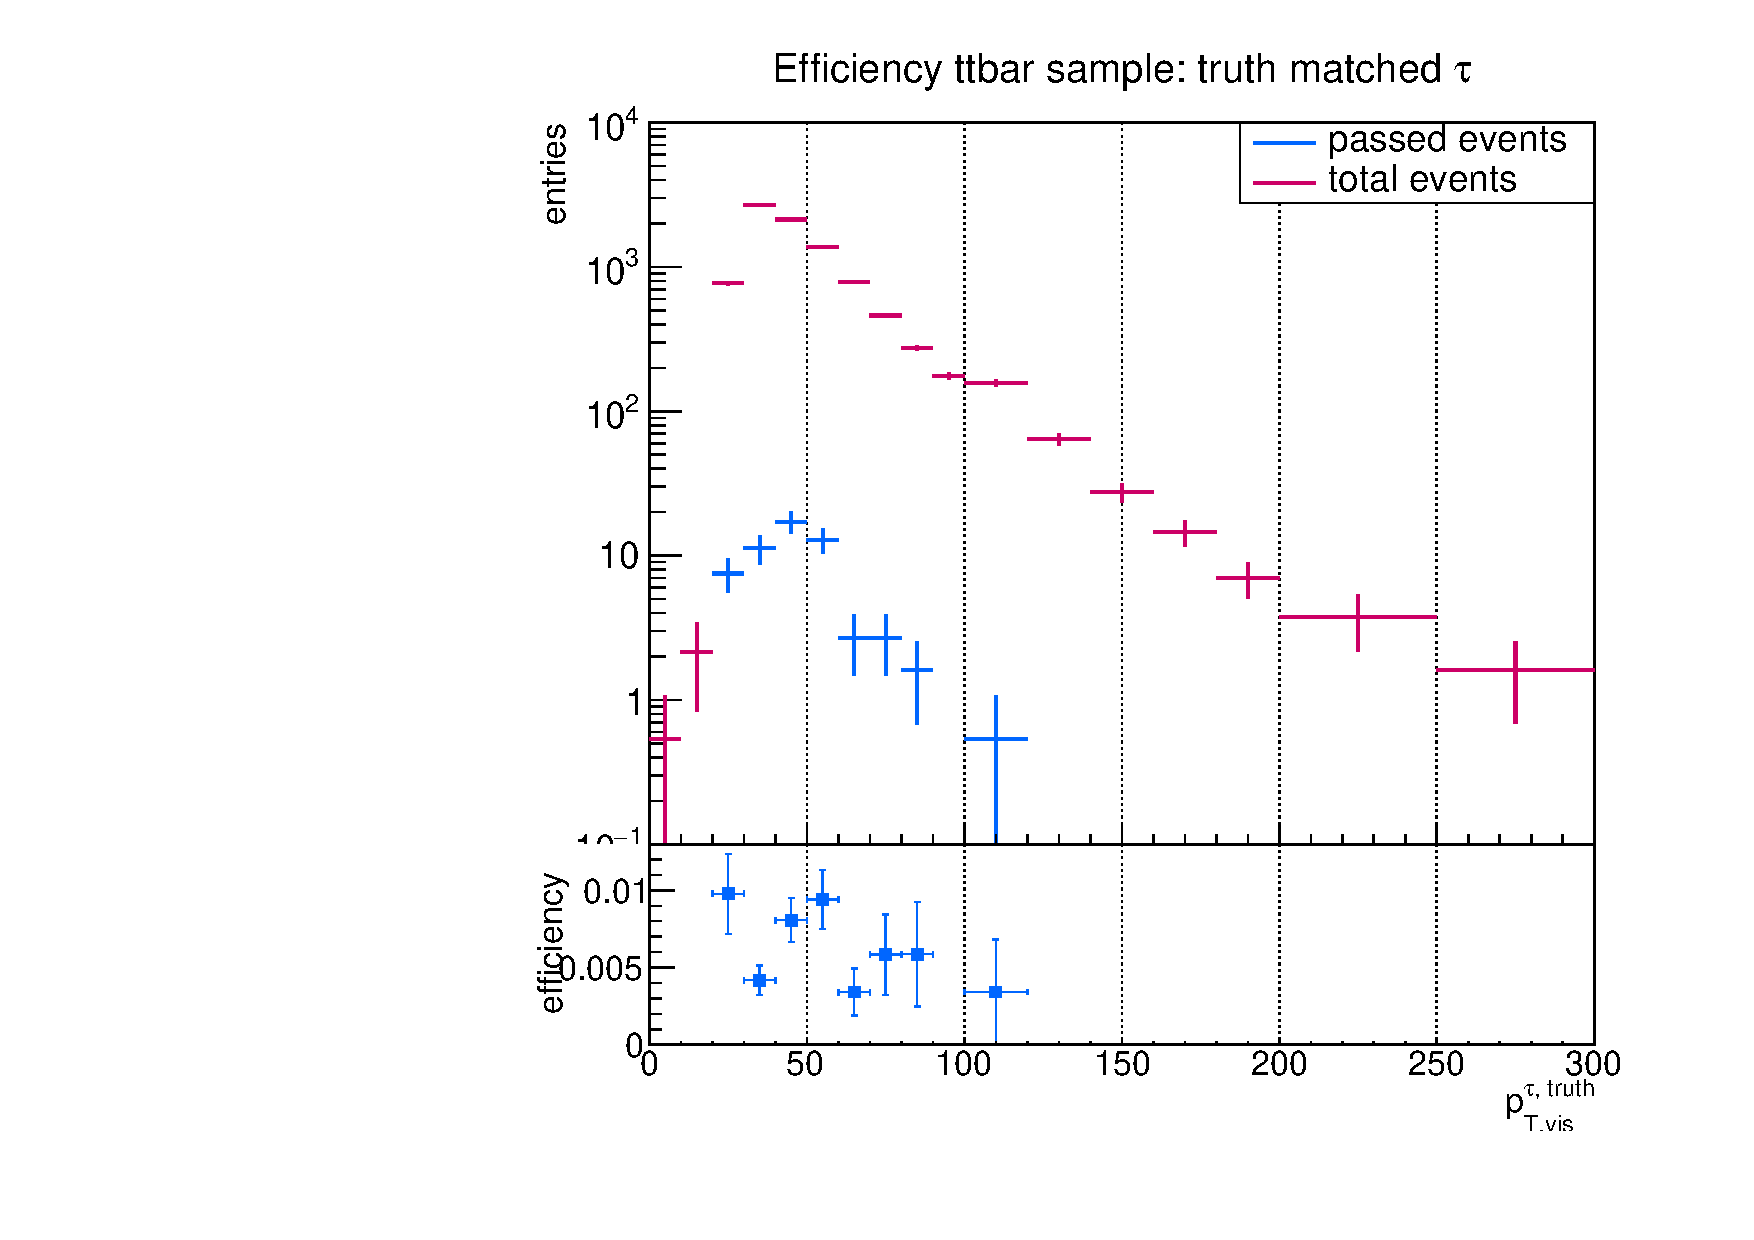
\includegraphics[width=\textwidth]{figures/plots/ttbar/Divided_Tau.pdf}
%                \subcaption{Hadronic tau reconstruction efficiency of $\SI{0.635\pm 0.061}{\percent}$ for the top-quark pair events.}
 %               \label{DividedTau:bg:ttbar}
 %               \end{subfigure}
 %               %
 %               \begin{subfigure}[t]{0.49\textwidth}
 %               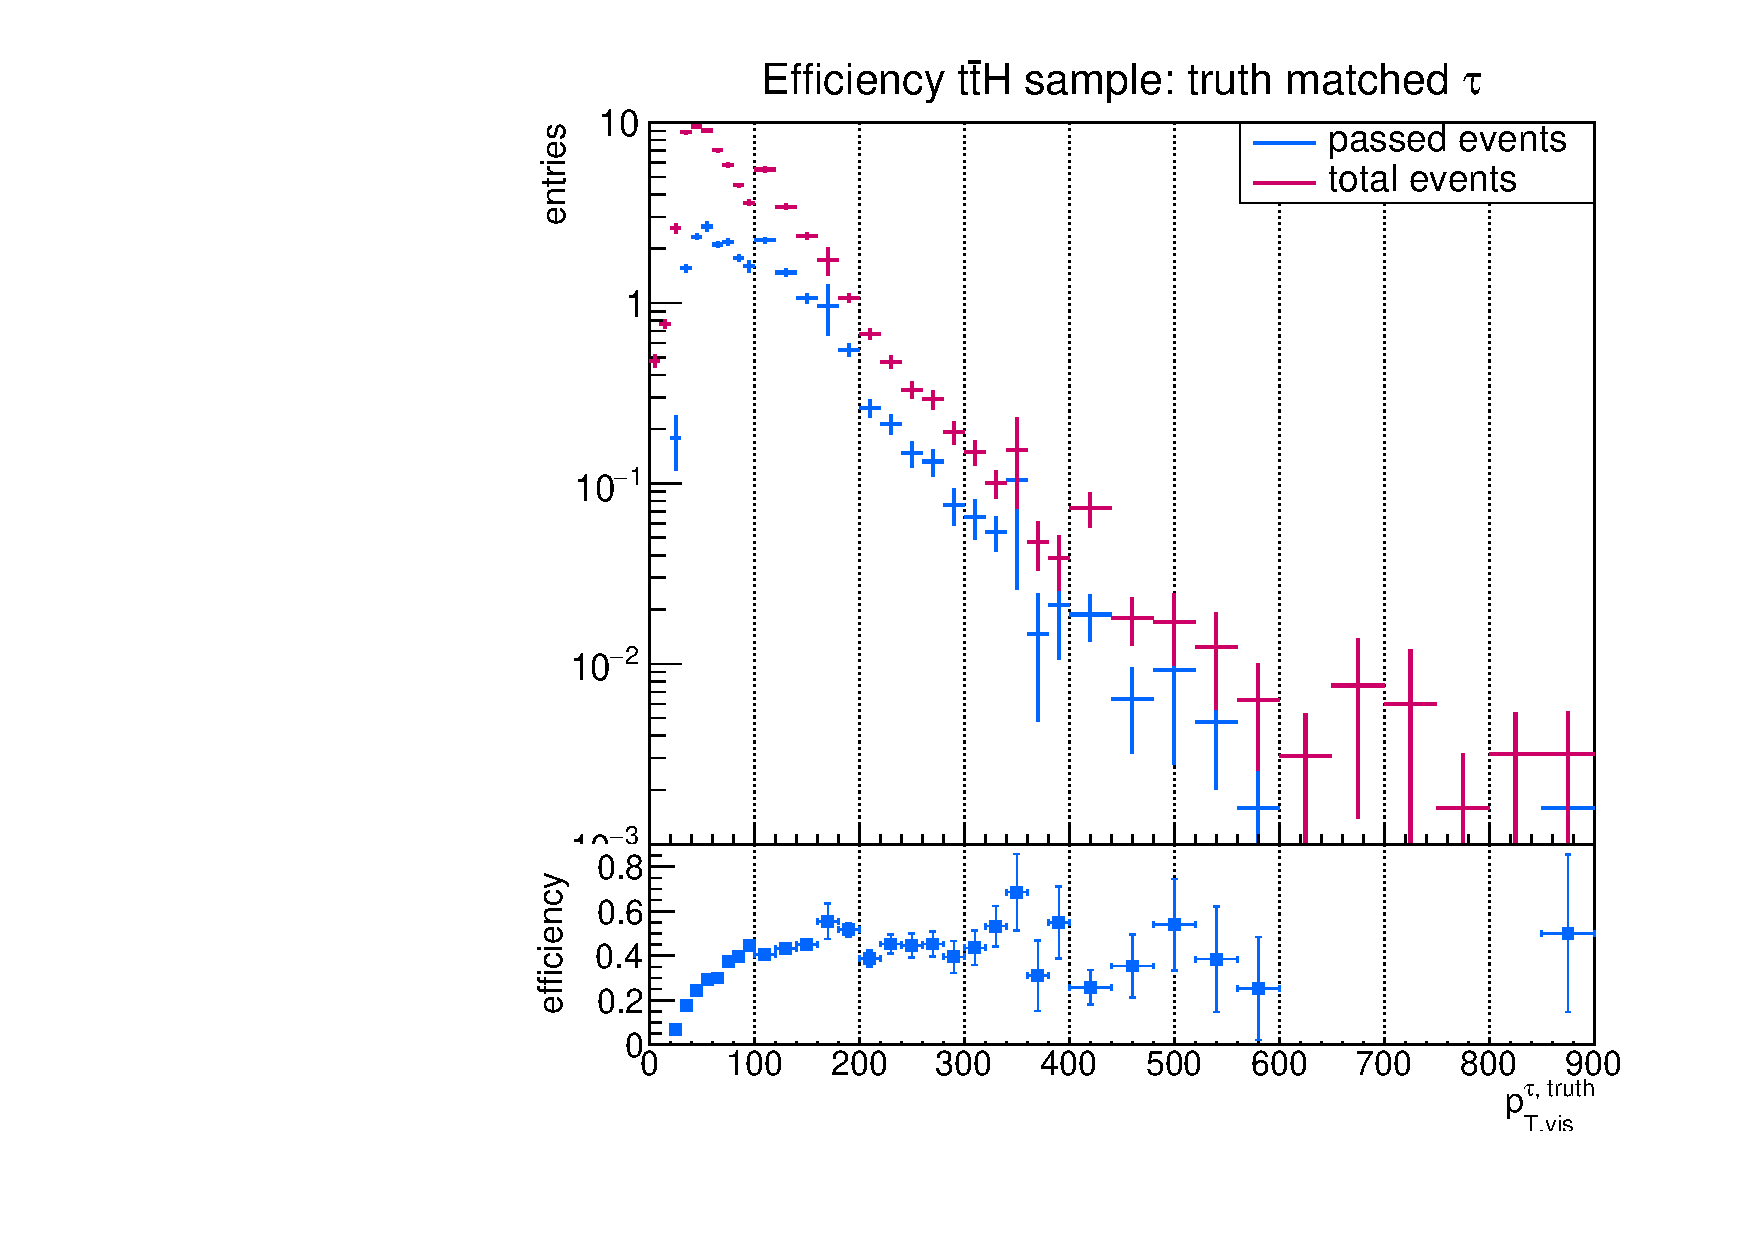
\includegraphics[width=\textwidth]{figures/plots/ttH/Divided_Tau.pdf}
 %               \subcaption{Hadronic tau reconstruction efficiency of $\SI{29.39\pm 0.26}{\percent}$ for the Higgs events.}
 %               \label{DividedTau:bg:ttH}
 %               \end{subfigure}
%\caption[Hadronic tau reconstruction efficiency for the background events.]{Hadronic tau reconstruction efficiency for the background events. The efficiency is defined as number of reconstructed hadronic taus passing the basic selection and is matched to a truth tau over the number of truth taus passing the basic selection (truth matching tau).}
%\label{DividedTau:bg}
%\end{figure}
%
%Jet
 The fake rate for jets that is the number of truth jets matched with a reconstructed tau-jet over the number of truth jets satisfying the basic selection is $\SI{0.1741\pm 0.0019}{\percent}$ and $\SI{1.0063\pm 0.0068}{\percent}$ for the top-pair related background and the Higgs related background respectively.\newline
The efficiency depending on the transverse momentum of the truth jet is shown as ratio plot in figure \ref{DividedJet:bg}.
%
\begin{figure}
  \centering
                \begin{subfigure}[t]{0.49\textwidth}
                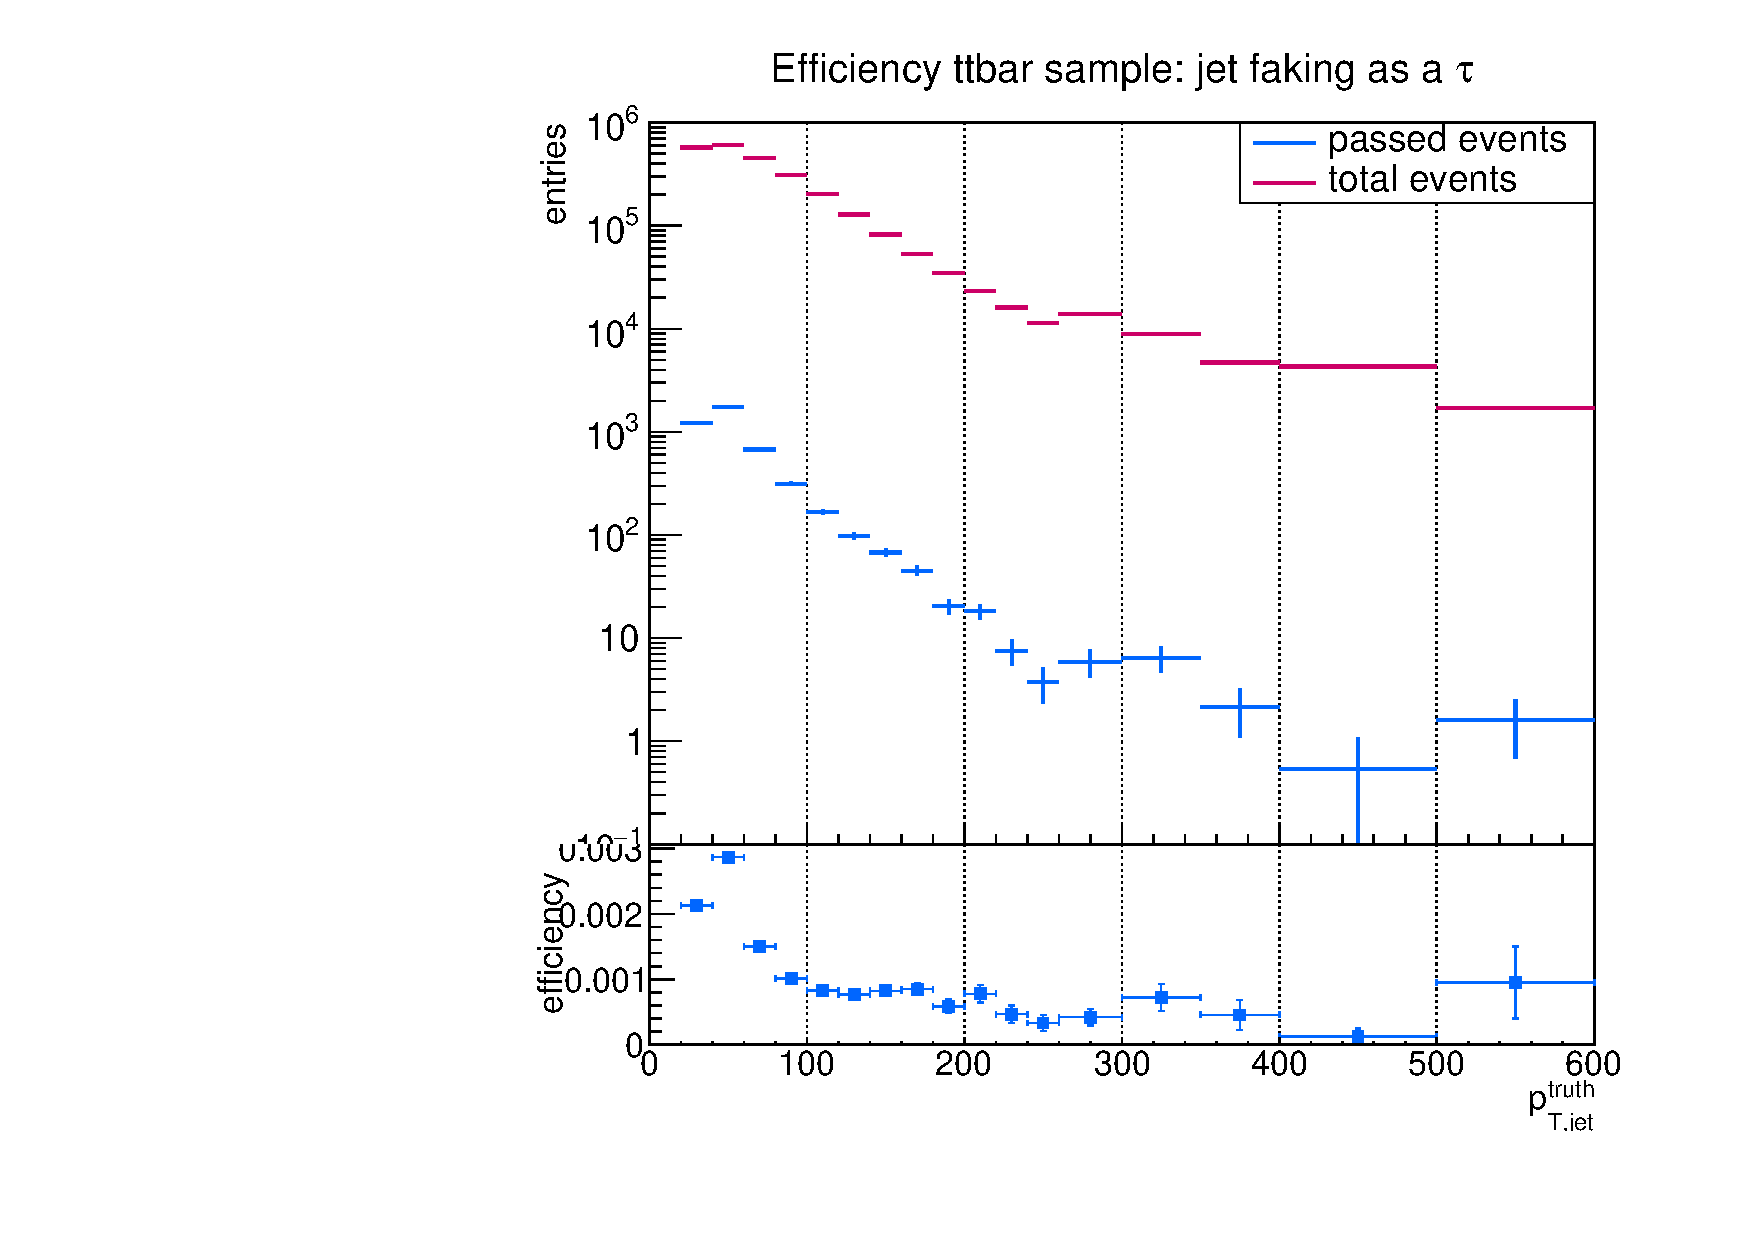
\includegraphics[width=\textwidth]{figures/plots/ttbar/Divided_Jet.pdf}
                \subcaption{Estimation of a jet faking a tau lepton of $\SI{0.1741\pm 0.0019}{\percent}$ for the top-quark pair events.}
                \label{DividedJet:bg:ttbar}
                \end{subfigure}
                %
                \begin{subfigure}[t]{0.49\textwidth}
                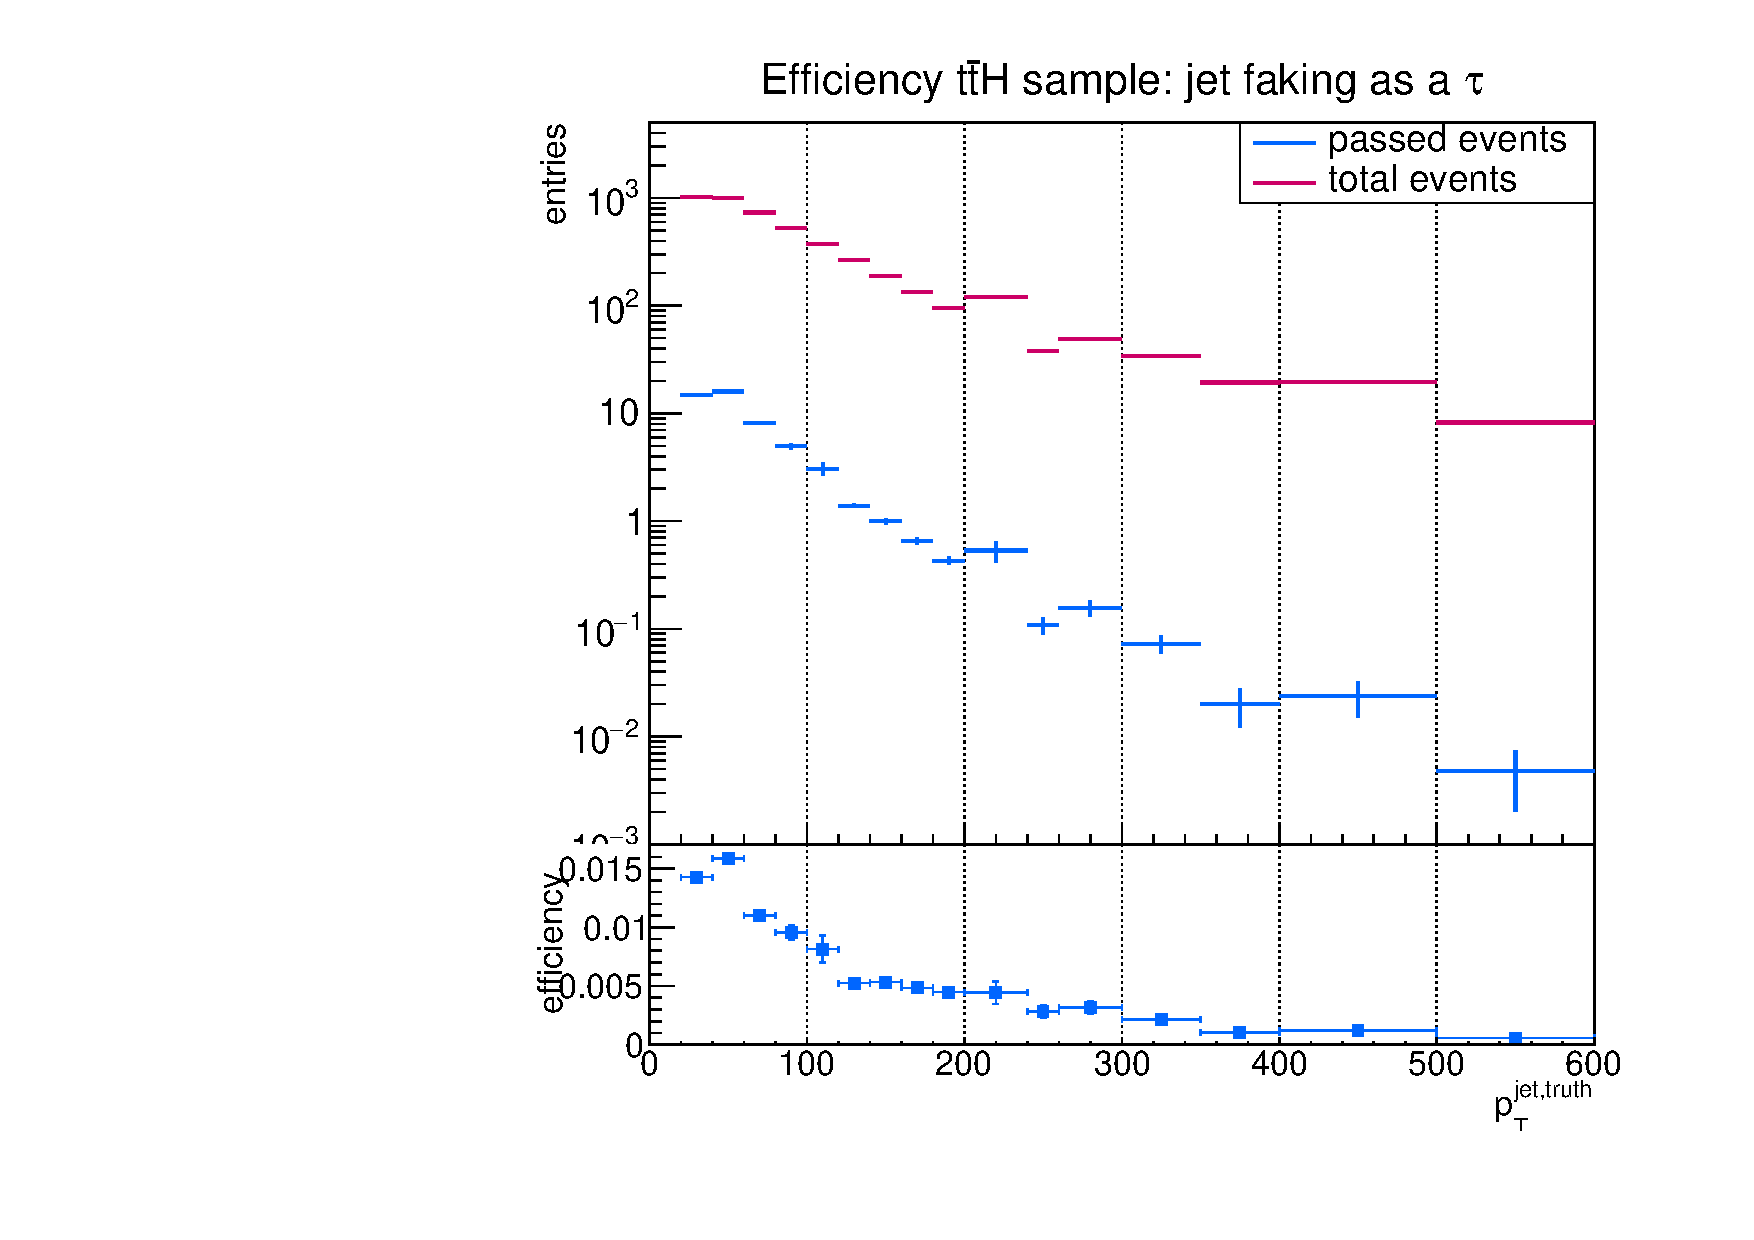
\includegraphics[width=\textwidth]{figures/plots/ttH/Divided_Jet.pdf}
                \subcaption{Estimation of a jet faking a tau lepton of $\SI{1.0063\pm 0.0068}{\percent}$ for the Higgs events.}
                \label{DividedJet:bg:ttH}
                \end{subfigure}        
\caption[Estimation of a jet faking a tau lepton for the background events.]{Estimation of a jet faking a tau lepton for the background events. The efficiency is defined as number of truth jets passing matched to a tau-jet over the number of truth jets passing the basic selection.}
\label{DividedJet:bg}
\end{figure}
%
The qualitative trend is for both background samples the same, showing a peak fake rate at $p_{T,\text{jet}}^{\text{truth}}$ at $\SI{50}{\giga\electronvolt}$. There exists a plateau in the range of the truth jet transverse momentum between $\SI{100}{\giga\electronvolt}$ and $\SI{200}{\giga\electronvolt}$ before the efficiency goes down. As a result the jet fake rate depends directly on the jets' transverse momentum. The main difference is that the fake rate for the $t\bar{t}H$ sample is greater than that of the $t\bar{t}$ sample. These differences in the mean fake rate could be due to the difference in jet composition. For $t\bar{t}$ the jets are gluon-originated (cf. fig. \ref{ttbarproduction}) and for $t\bar{t}H$ quark-originated (cf. fig. \ref{ttHproduction}) jets.\par
%b-jet
The fake rate for b-jets is defined in the same way as for jets above with the difference of selecting only jets of b-flavor. The fake rate values of the two background samples are not in agreement within the uncertainties, Although they are in the same range of $\SI{0.1616\pm 0.0022}{\percent}$ and $\SI{0.1496\pm 0.0033}{\percent}$ corresponding to $t\bar{t}$ and $t\bar{t}H$. The efficiency depending on the truth transverse momentum of the b-jet is shown in figure \ref{DividedBjet:bg}.
%
\begin{figure}
  \centering
                \begin{subfigure}[t]{0.49\textwidth}
                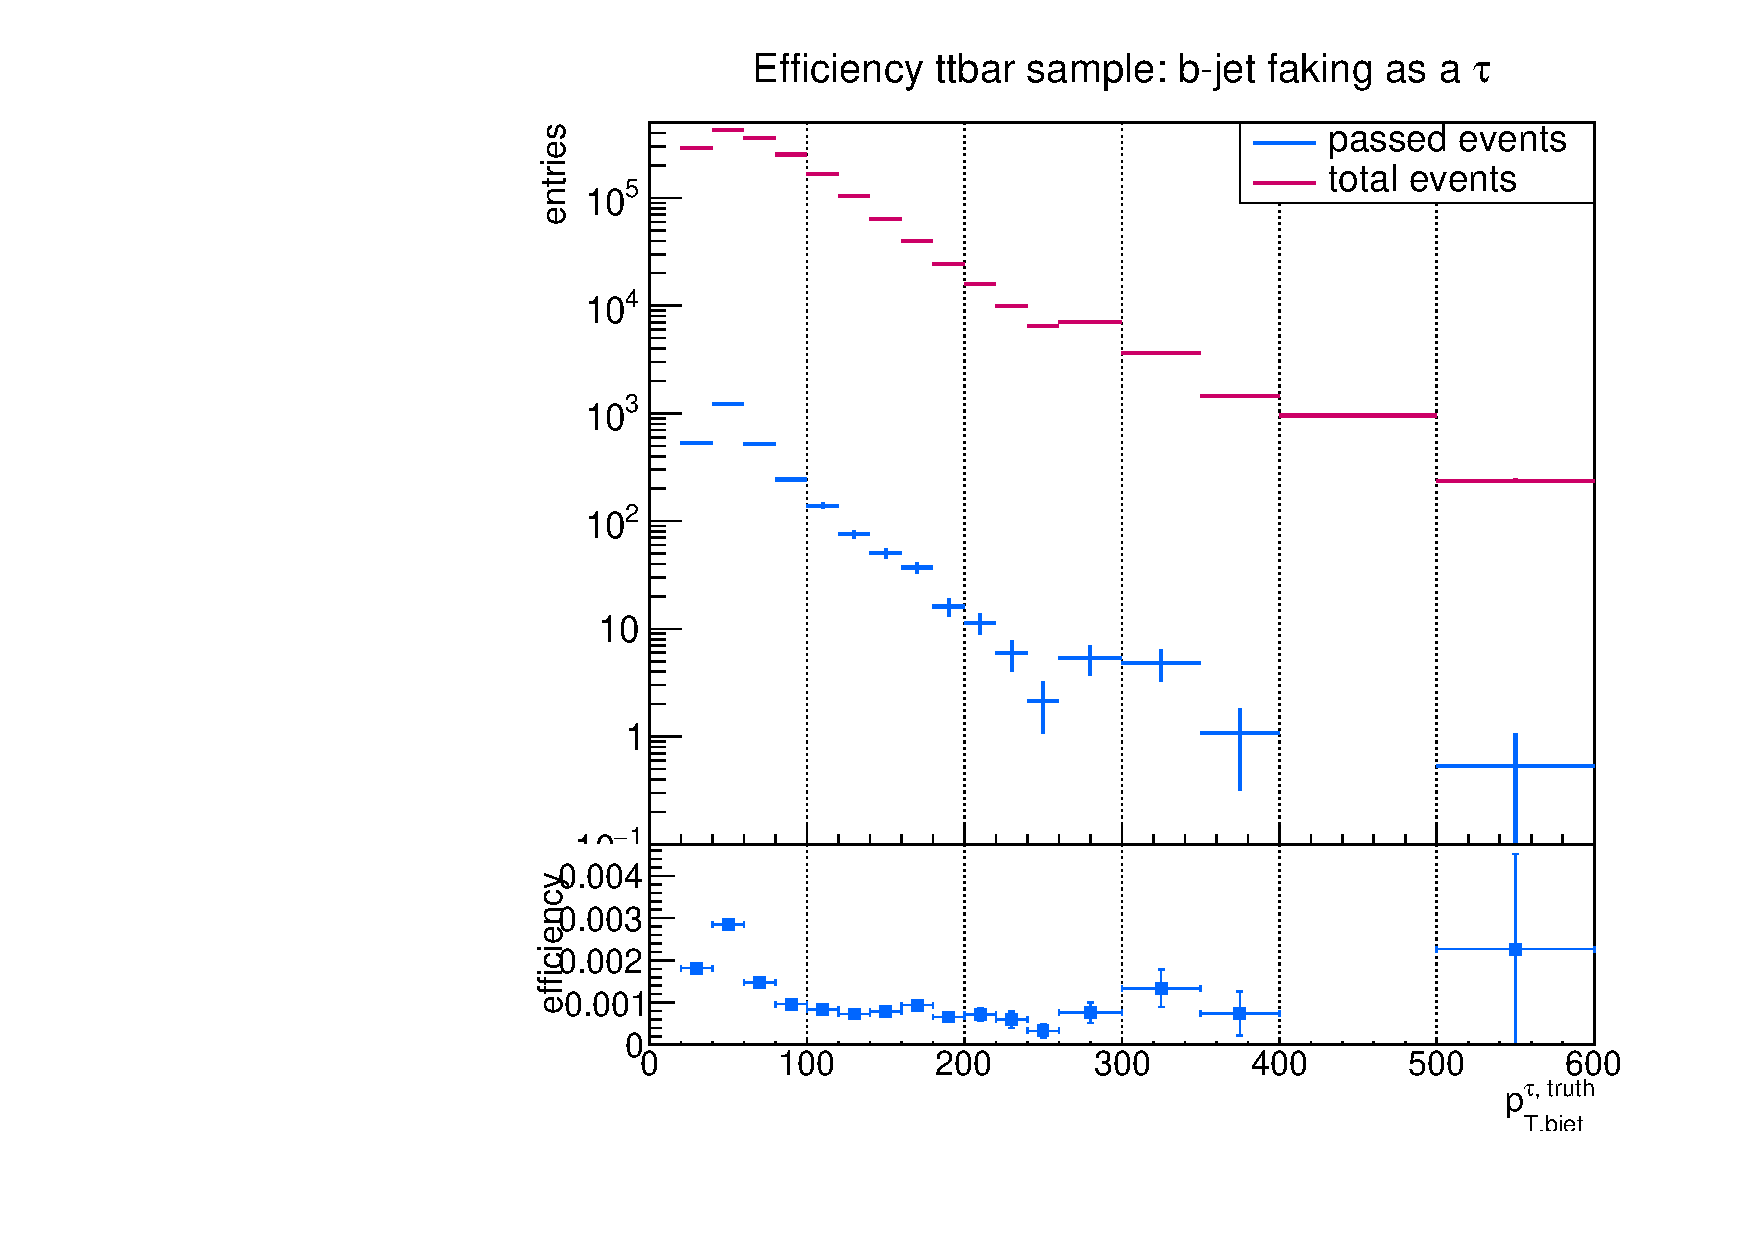
\includegraphics[width=\textwidth]{figures/plots/ttbar/Divided_Bjet.pdf}
                \subcaption{Estimation of a b-jet faking a tau lepton of $\SI{0.1616\pm 0.0022}{\percent}$ for the top-quark pair events.}
                \label{DividedBjet:bg:ttbar}
                \end{subfigure}
                %
                \begin{subfigure}[t]{0.49\textwidth}
                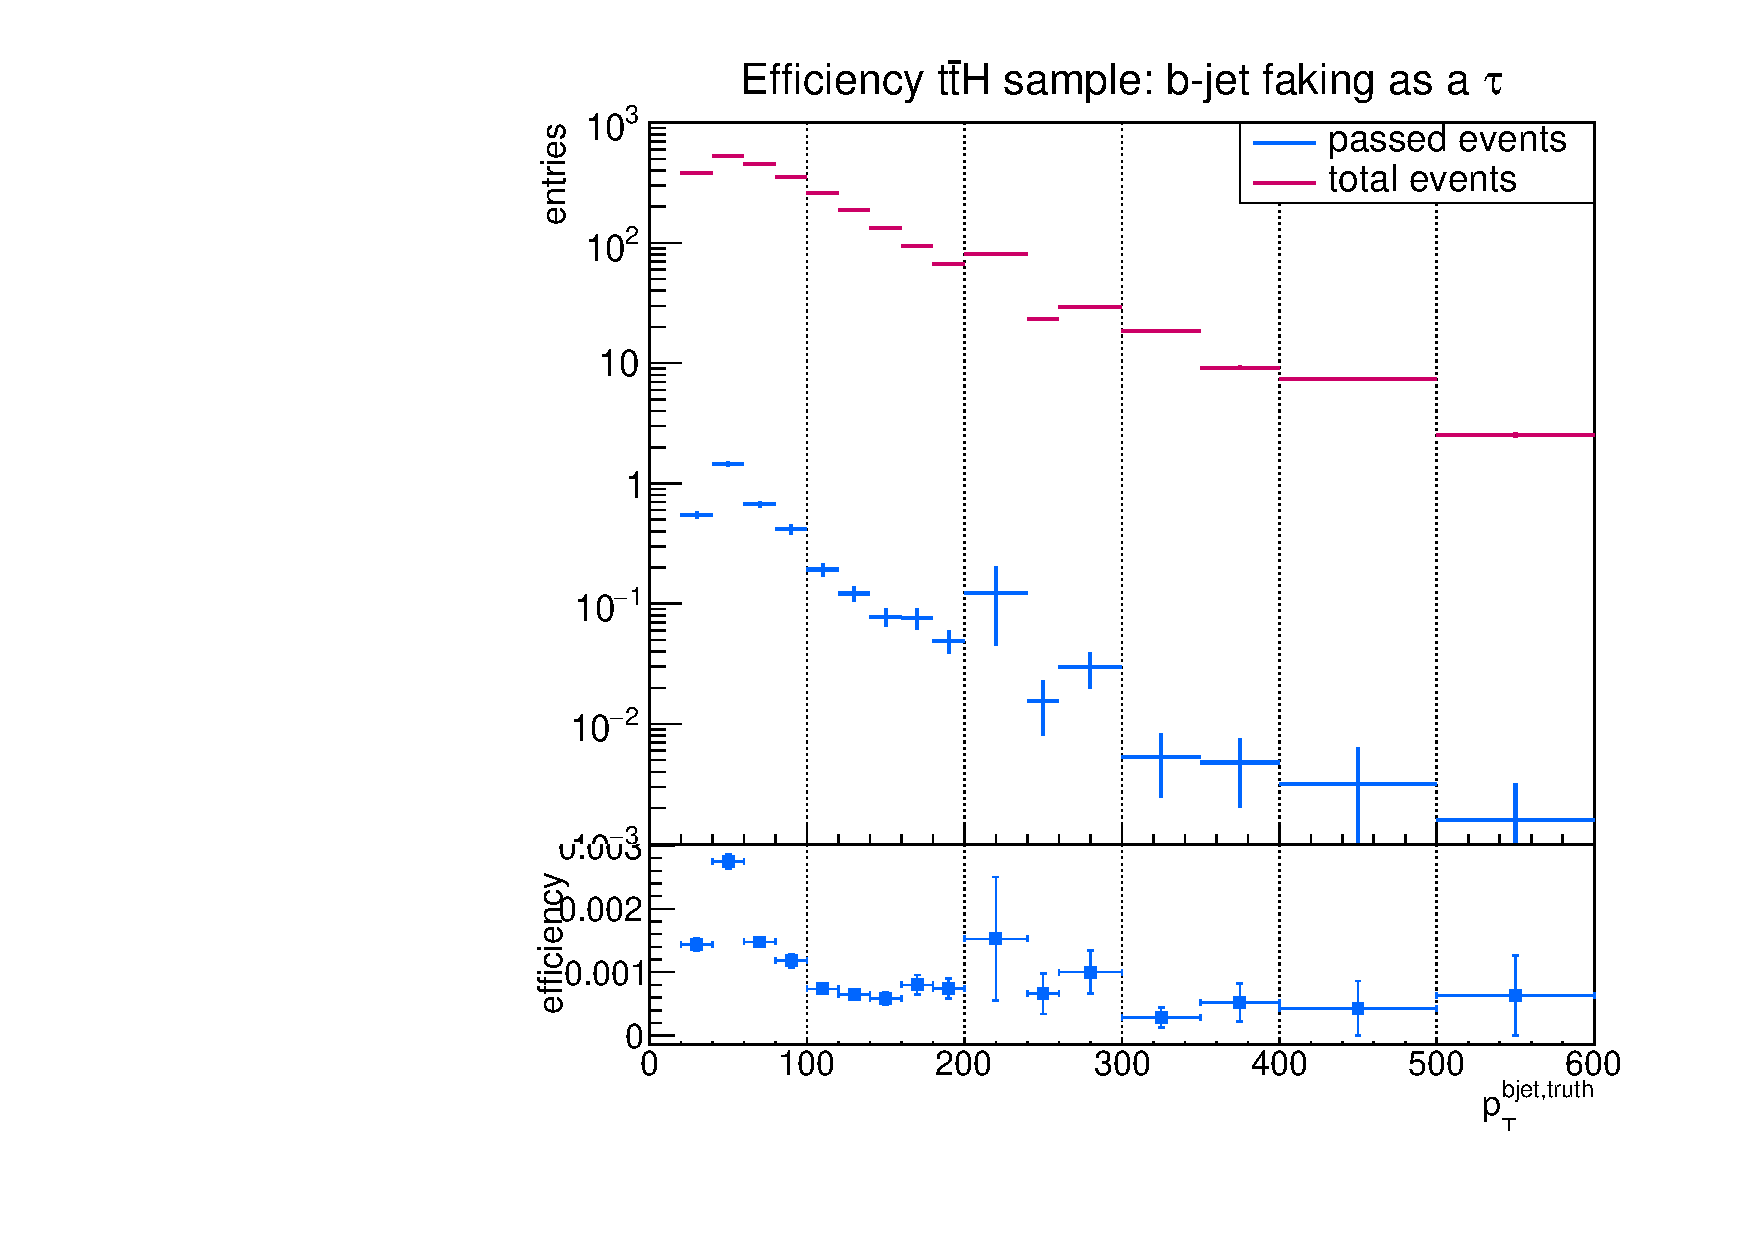
\includegraphics[width=\textwidth]{figures/plots/ttH/Divided_Bjet.pdf}
                \subcaption{Estimation of a b-jet faking a tau lepton of $\SI{0.1496\pm 0.0033}{\percent}$ for the Higgs events.}
                \label{DividedBjet:bg:ttH}
                \end{subfigure}
\caption[Estimation of a b-jet faking a tau lepton for the background events.]{Estimation of a b-jet faking a tau lepton for the background events. The efficiency is defined as number of truth b-jets matched to a tau-jet over the number of truth b-jets passing the basic selection.}
\label{DividedBjet:bg}
\end{figure}
%
The dependence of the fake rate in case of b-jets faking a tau follows the same trend as observed for jets in general. The only difference is that the b-jet fake rate in the Higgs sample is slightly higher compared to the top-pair sample. This fact can be explained by the $p_T$ dependence of the fake rate: The b-jet's $p_T$ spectrum is slightly harder in the Higgs sample (see fig. \ref{DividedBjet:bg:ttH}) compared to the top-pair sample (see fig. \ref{DividedBjet:bg:ttbar}).
%NoBjet
To complete the view on jet composition the next fake cadidates are light jets explicitly excluding b-jets and their corresponding fake rate plot is shown in figure \ref{DividedNoBjet:bg}. The fake rate is $\SI{0.2034\pm 0.0038}{\percent}$ and $\SI{2.356\pm 0.016}{\percent}$ for $t\bar{t}$ and $t\bar{t}H$ sample respectively. As the ratio plot shows, the fake rate is high for the background contributions related to Higgs in the a greater range up to $\SI{120}{\giga\electronvolt}$, whereas the background contributions related to the top-pair events show the characteristic peak at \SI{50}{\giga\electronvolt} as observed earlier. The difference in the fake rate, where light jets fake as tau is consistent with the above mentioned fact that the jet composition and therefore the light jet composition is different in both background samples.\par
%
\begin{figure}
  \centering
                \begin{subfigure}[t]{0.49\textwidth}
                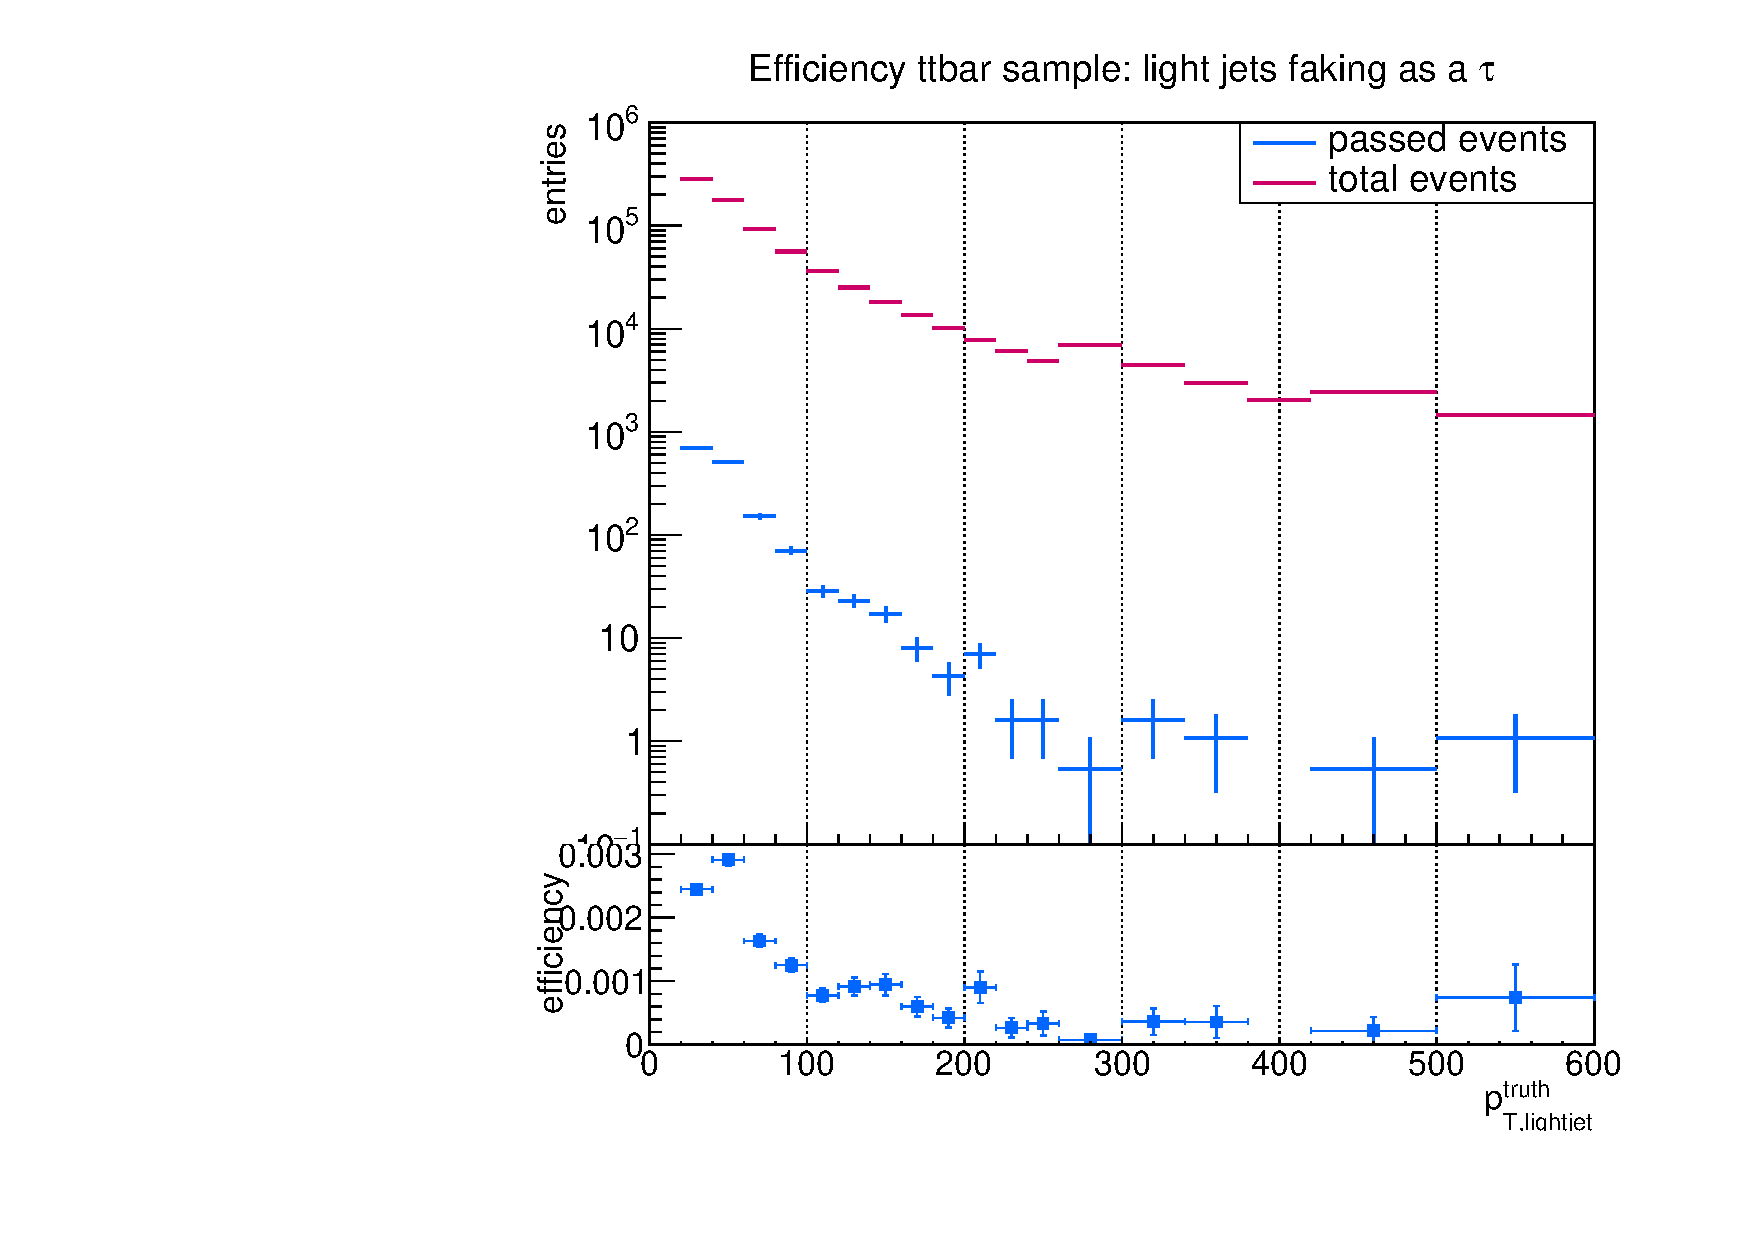
\includegraphics[width=\textwidth]{figures/plots/ttbar/Divided_NoBjet.pdf}
                \subcaption{Estimation of a light jet (excluding b-jets) faking a tau lepton of $\SI{0.2034\pm 0.0038}{\percent}$ for the top-quark pair events.}
                \label{DividedNoBjet:bg:ttbar}
                \end{subfigure}
                %
                \begin{subfigure}[t]{0.49\textwidth}
                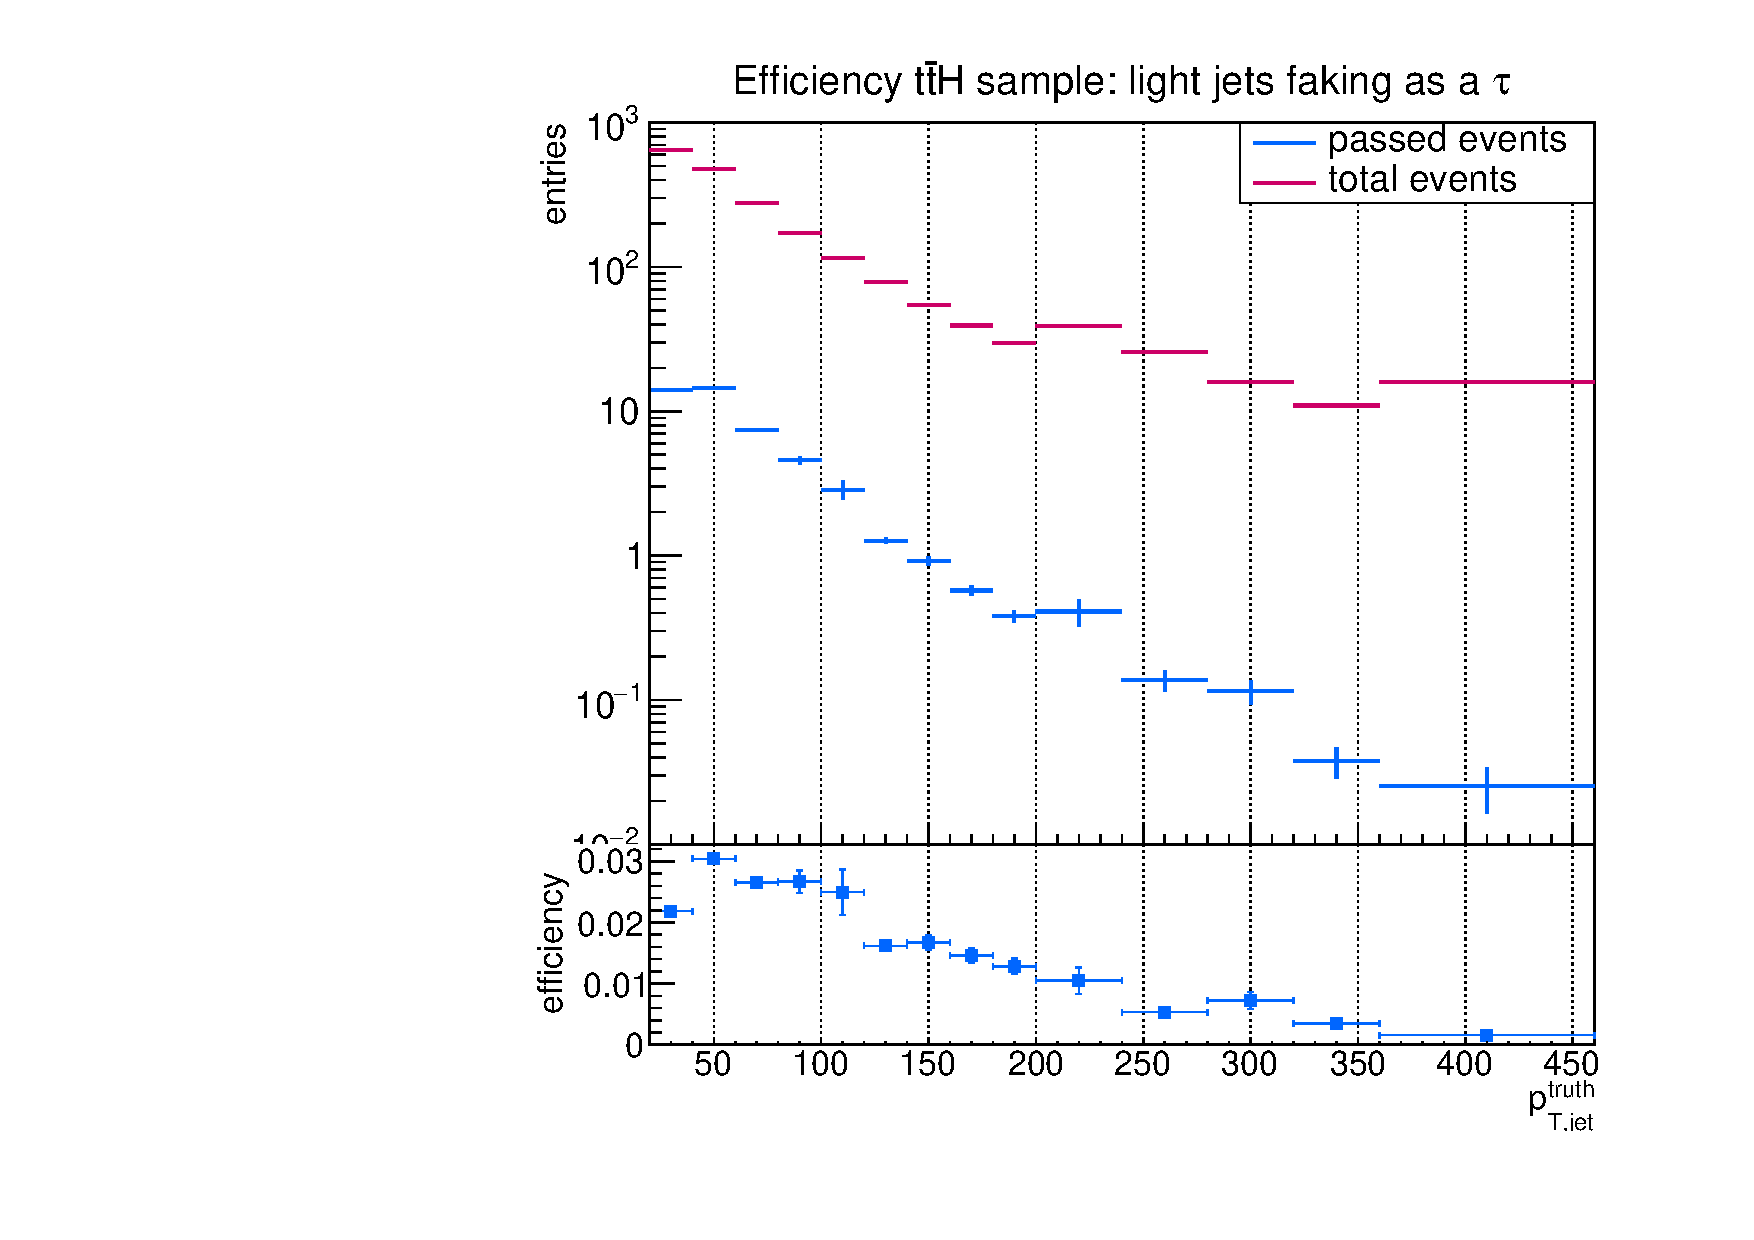
\includegraphics[width=\textwidth]{figures/plots/ttH/Divided_NoBjet.pdf}
                \subcaption{Estimation of a light jet (excluding b-jets) faking a tau lepton of $\SI{2.356\pm 0.016}{\percent}$ for the Higgs events.}
                \label{DividedNoBjet:bg:ttH}
                \end{subfigure}
   %             
\caption[Estimation of a light-jet faking a tau lepton for the background events.]{Estimation of a light-jet (excluding b-jets) faking a tau lepton for the background events. The efficiency is defined as truth number of light jets, explicitly not including the b-flavor, matched to a tau-jet over the number of truth light jets without truth b-jets passing the basic selection.}
\label{DividedNoBjet:bg}
\end{figure}
%
%e fake 
The fake tau contributions from electrons is very tiny in this efficiency consideration. The fake rate estimation is done by taking the true number of electrons, which are reconstructed as a hadronic tau over the truth electrons passing the basic selection. For the top-pair related events the fake rate is $\SI{0.00104\pm 0.00025}{\percent}$ and for the Higgs related events $\SI{0.00348\pm 0.00084}{\percent}$.\par
%One reason for such a low rate lies in the standard procedure of tau reconstruction described in section \ref{taus}, where most of the electrons are already vetoed. \par das passt scheinbar nicht??
%
%
%
%
%
%	
\begin{table}[htbp]
		\centering
                \footnotesize
                \renewcommand{\arraystretch}{1.2}
		\begin{tabular*}{\linewidth}{@{\extracolsep{\fill}}ccc}
		\hline
                \hline
		\textbf{sample}    & \multicolumn{2}{c}{\textbf{t$\bar{\textbf{t}}$H}} 
		\\
		\hline
		\multirow{2}{*}{selection}   & reconstructed taus       & total number
                \\
                & matched to truth taus & of taus
		\\ 
		\hline
                tau originated from H$^0$        & $5140$          & $11372$
		\\
		efficiency                     & \multicolumn{2}{c}{$\SI{45.20\pm 0.47}{\percent}$}
		\\
		\hline
                tau originated from H$^0$ (1-prong)         & $4132$          & $8390$
		\\
		efficiency                     & \multicolumn{2}{c}{$\SI{49.25\pm 0.55}{\percent}$}
		\\
		\hline
                tau originated from H$^0$ (3-prong)         & $1008$          & $2958$
		\\
		efficiency                    & \multicolumn{2}{c}{$\SI{34.08\pm 0.87}{\percent}$}
		\\
		\hline
		\hline
		\end{tabular*}
		\caption[Efficiencies for the t$\bar{\text{t}}$H sample.]{Efficiencies for different tau lepton categories for the t$\bar{\text{t}}$H Monte Carlo sample. The efficiency is defined as $\epsilon=\frac{\text{\#truth hadronic }\tau\text{ matched to a reconstructed }\tau+Z}{\text{\#truth }\tau\text{ passing the basic selection}+Z}$.}
		\label{ttbarttHEffTable}
          \renewcommand{\arraystretch}{1}
\end{table}
%
% H für Higgs Betrachtung
As discussed in section \ref{MCsamples} the advantage of the $t\bar{t}H$ sample is that it includes real tau signals. Therefore tau efficiency study is not only possible for the signal samples, but can be studied as well of the background is done here for the $t\bar{t}H$ sample. The efficiency definition was already given with eq. (\ref{effeq}) at the beginning of this section. To determine the tau efficiency further sub-selections shown in table \ref{ttbarttHEffTable} are performed.\newline
Two main sources of taus can be distinguished and include both the sub-categories of 1-prong and 3-prong decays (cf. \ref{startingpoint} and \ref{taus}): Taus originating from bosons of the weak interaction ($W^\pm$, $Z^0$) and taus originating directly from Higgs bosons. This variety comes with the diversity of the Higgs decay modes like di-boson and di-tau events. Applied overlap removals between tau leptons and light leptons (see section \ref{overlapremoval}) reduce the efficiency numbers significantly. Therefore only taus from $H^0$ are considered. %Nevertheless the plots for tau leptons originating from $W^\pm$ and $Z^0$ can be found in section \ref{promptplots}. 
%
%Selecting the number of taus passing the basic selection and are matched to a truth tau within $\Delta R=0.05$ originating from weak bosons over the total number of truth taus passing the basic selection and originate from weak bosons gives an efficiency value of $\SI{36.76\pm 0.51}{\percent}$. Higgs decaying into vector bosons gives rise to this proportion of the tau leptons. The dependency of the efficiency with the transverse momentum of the truth tau is shown in figure \ref{Dividedprompt:bg:all}. Splitting this origin into 1-prong and 3-prong case of the subsequent tau decay gives efficiency values of $\SI{40.16\pm 0.62}{\percent}$ and $\SI{29.01\pm 0.88}{\percent}$ respectively (see figure \ref{Dividedprompt:bg:1prong} and \ref{Dividedprompt:bg:3prong}). The efficiencies for the tau reconstruction after one charged particle or three charged particles are reasonable when compared to the reconstruction efficiencies of the selected physical objects. Taking into account $\sim\SI{99}{\percent}$ of the muon and electron reconstruction efficiency \cite{muPerformance}\cite{ePerformance2}, the two b-jets with a reconstruction efficiency of $\SI{77}{\percent}$ each (cf. section \ref{btagging} and \ref{physObj:bjet}) and the reconstruction efficiency of a loose tau with $\SI{60}{\percent}$ (1-prong) and $\SI{50}{\percent}$ (3-prong) (cf. section \ref{taus}). Following the product of the reconstruction efficiencies $\epsilon_{1/3-\text{prong}}=\epsilon_e\epsilon_\mu\epsilon_{2\text{b-jets}}\epsilon_\tau$ results in $\SI{35}{\percent}$ (1-prong) and $\SI{29}{\percent}$ (3-prong).\newline
%
% XXXXXXXXXXXXXXXXXXXXXXXXx
%

%
%
%
The efficiency derived from the number of taus matched to a truth tau and originating from a Higgs boson over the total number of truth taus passing the basic selection and its origin from Higgs is $\SI{45.20\pm 0.47}{\percent}$. The efficiency plot is shown in figure \ref{DividedFromH:bg:all}. Splitting the taus' origin from $H^0$ into 1-prong and 3-prong case gives the efficiency of $\SI{49.25\pm 0.55}{\percent}$ and $\SI{34.08\pm 0.87}{\percent}$ respectively (see figure \ref{DividedFromH:bg:1prong} and \ref{DividedFromH:bg:3prong}). %Compared to the efficiency resulting from the product of the different object reconstruction efficiencies the tau efficiency coming from Higgs decays are 15 percentage points and 5 percentage point higher for the 1-prong and 3-prong case respectively.\par
The overall efficiency dependence increases towards $\SI{200}{\giga\electronvolt}$ and fluctuates beyond that threshold for higher transverse momenta. This behavior is mostly dominated by the 1-prong cases with its highest contribution to the prompt Higgs decay, because the 1-prong case in figure \ref{DividedFromH:bg:1prong} shows the same trend. In contrast to that, the smaller contributions of $\SI{34.08\pm 0.87}{\percent}$ efficiency in the 3-prong case show slightly less dependence in efficiency (see fig. \ref{DividedFromH:bg:3prong}).\par
%
\begin{figure}
  \centering
                \begin{subfigure}[t]{0.49\textwidth}
                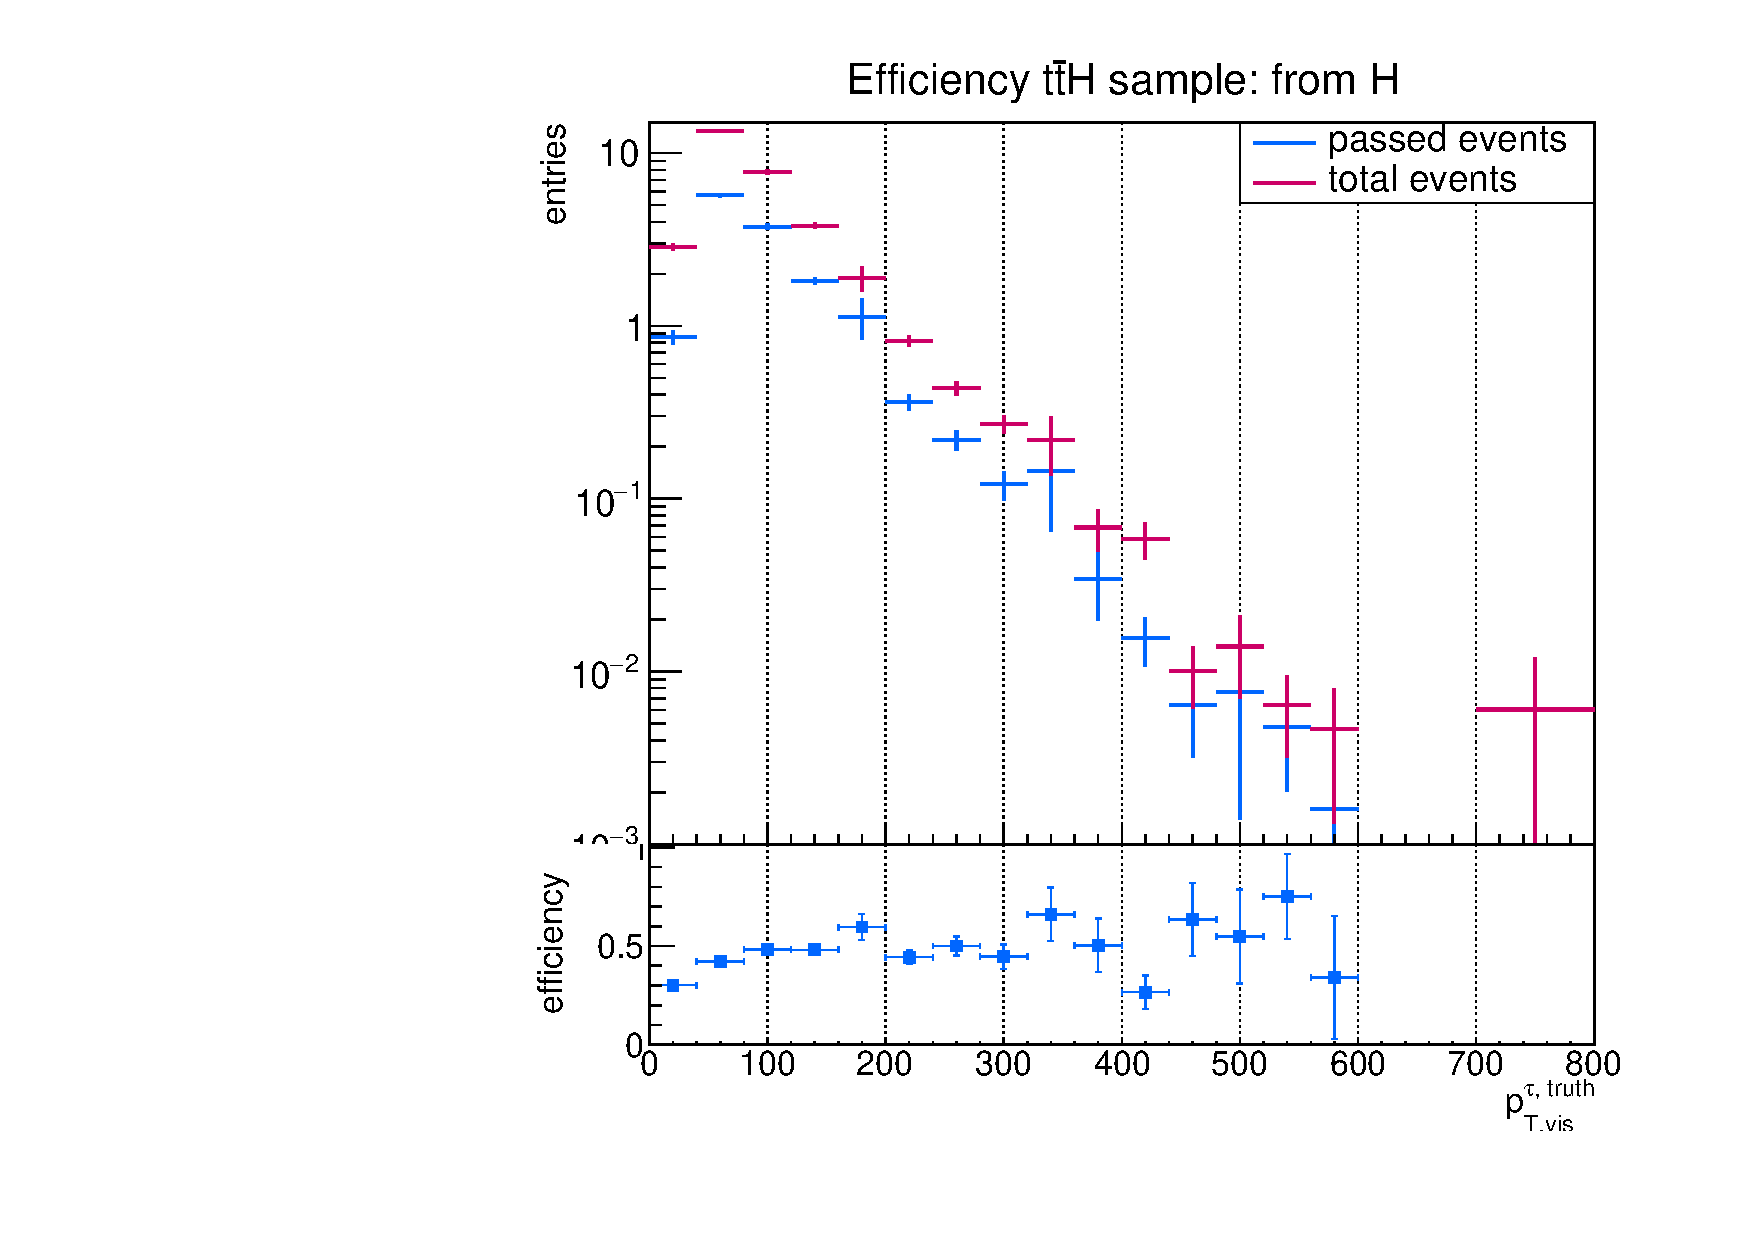
\includegraphics[width=\textwidth]{figures/plots/ttH/Divided_H.pdf}
                \subcaption{Efficiency of taus originating from Higgs bosons  of $\SI{45.20\pm 0.47}{\percent}$ for the Higgs events.}
                \label{DividedFromH:bg:all}
                \end{subfigure}
                %
                \begin{subfigure}[t]{0.49\textwidth}
                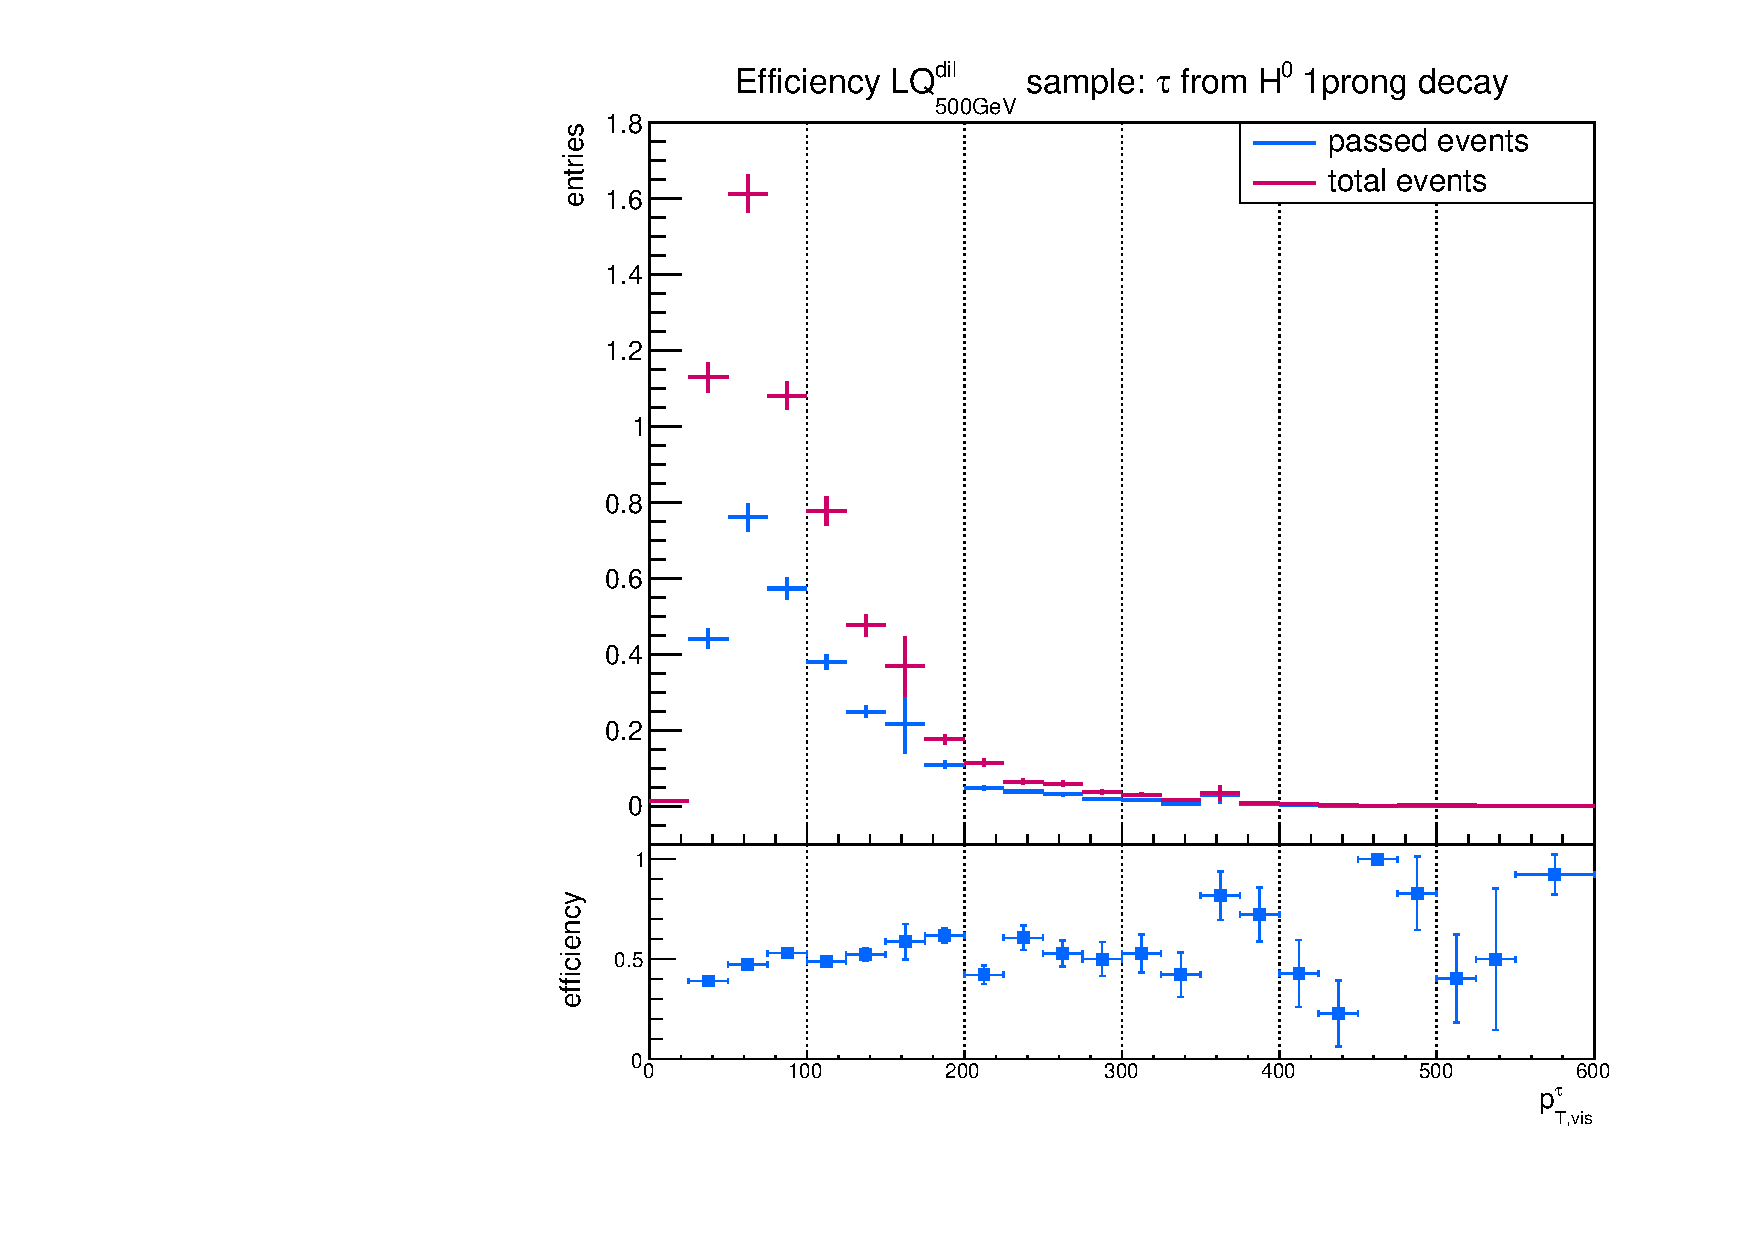
\includegraphics[width=\textwidth]{figures/plots/ttH/Divided_fromH1prong.pdf}
                \subcaption{Efficiency of taus originating from Higgs bosons and decaying in the 1-prong mode. The efficiency is $\SI{49.25\pm 0.55}{\percent}$ for the Higgs events.}
                \label{DividedFromH:bg:1prong}
                \end{subfigure}
                %
                \begin{subfigure}[t]{0.49\textwidth}
                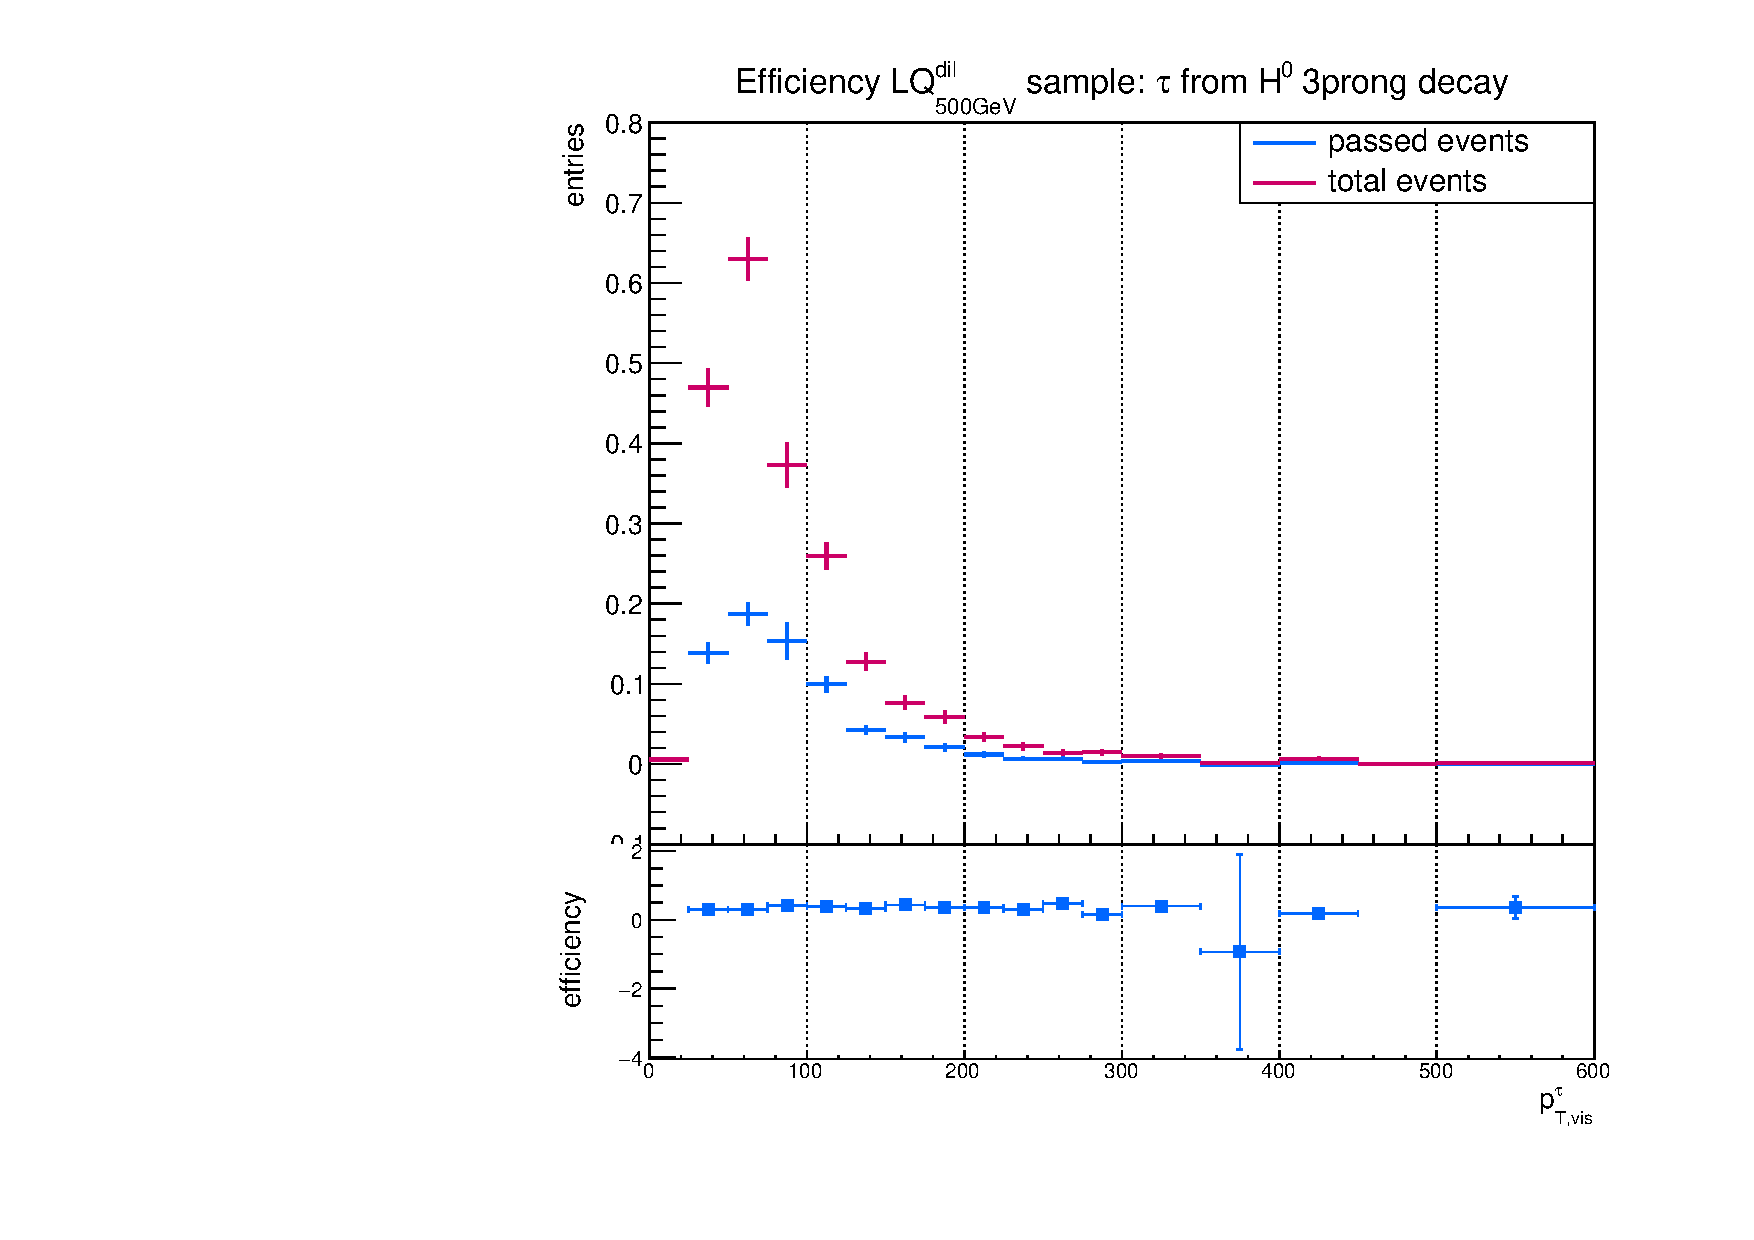
\includegraphics[width=\textwidth]{figures/plots/ttH/Divided_fromH3prong.pdf}
                \subcaption{Efficiency of taus originating from Higgs bosons and decaying in the 3-prong mode. The efficiency is $\SI{34.08\pm 0.87}{\percent}$ for the Higgs events.}
                \label{DividedFromH:bg:3prong}
                \end{subfigure}
   %             
\caption[Efficiency of taus originating from Higgs bosons.]{Efficiency of taus originating from Higgs. The efficiency is defined as the number of taus matched to a hadronic truth tau as well as the origin is from a $H^0$ boson over the total number of truth taus passing the basic selection and originating from a $H^0$ boson.}
\label{DividedFromH:bg:ttH}
\end{figure}
%
%from B mesons
%The dependency of the tau reconstruction efficiency are shown in figure \ref{DividedTau:bg}. The difficulty of the real tau reconstruction with transverse momenta smaller than $\sim\SI{100}{\giga\electronvolt}$ can be seen in the ratio plot of the Higgs sample with its low efficiency in that $p_{T,\text{vis}}^{\tau,\text{truth}}$ range (fig. \ref{DividedTau:bg:ttH}).
%Further investigating the matched truth tau`s origin shows that they originate from heavy B mesons (tau from B-mesons in \ref{ttbarttHEffTable}). This is denoted by the efficiency defined by the number of hadronic taus in the basic selection matched to a truth particle and originating from B-mesons over the total number of taus in the basic selection originating from B-mesons. Background contributions from Higgs events only originate only in rare cases from B-mesons with a efficiency of $\SI{0.514\pm 0.077}{\percent}$.\par
%Überleitung zu kinematic variables
The evaluated efficiencies of the sub-selection, where taus originate directly from Higgs, can also be expressed as a function of various kinematic variables, which is presented here for the $t\bar{t}H$ sample. The next section (\ref{signaleff}) provides this study for the LQ signal samples as well.\newline
%HT Gedöns// H 
Thus, as a reference for the LQ signal samples the sum of the transverse momenta of different physical variables $S_{T,\text{lep}}$, $H_{T,\text{had}}$, $S_{T}$, $H_{T}$ and the number of jets are plotted against the efficiency for taus originating from Higgs bosons. The definition of the sum-variables are as follows:
\begin{align}
S_{T,\text{lep}}&=\cancel{E}_{T}+\sum_i p_{T,i}^{\text{e}}+\sum_i p_{T,i}^{\mu}+\sum_i p_{T,i}^{\tau} \label{STlepgedöns}\\
H_{T,\text{had}}&=\sum_i p_{T,i}^{\text{jet}} \label{HThadgedöns}\\
S_{T}&=\cancel{E}_{T}+\sum_i p_{T,i}^{\text{e}}+\sum_i p_{T,i}^{\mu}+\sum_i p_{T,i}^{\tau}+\sum_i p_{T,i}^{\text{jet}} \label{STgedöns}\\
H_{T}&=\sum_i p_{T,i}^{\text{e}}+\sum_i p_{T,i}^{\mu}+\sum_i p_{T,i}^{\text{jet}}\,\text{,}
\label{HTgedöns}
\end{align}
where $p_{T,i}^\text{X}$ is the transverse momentum of single electrons $X=e$, muons $X=\mu$, taus $X=\tau$ and jets $X=\text{jet}$ and $\cancel{E}_{T}$ denotes the missing transverse energy, which includes in standard model considerations the neutrinos. With the definitions of eq. (\ref{STlepgedöns})-(\ref{HTgedöns}) different sensitivities are covered. $S_T$ is sensitive to all considered objects with the sub-category of $S_{T,\text{lep}}$, which only takes the leptonic objects into account, while $H_{T}$ is sensitive to electrons and muons as well as jets. $H_{T,\text{had}}$ only includes jets.\par
\begin{figure}
  \centering
                \begin{subfigure}[t]{0.49\textwidth}
                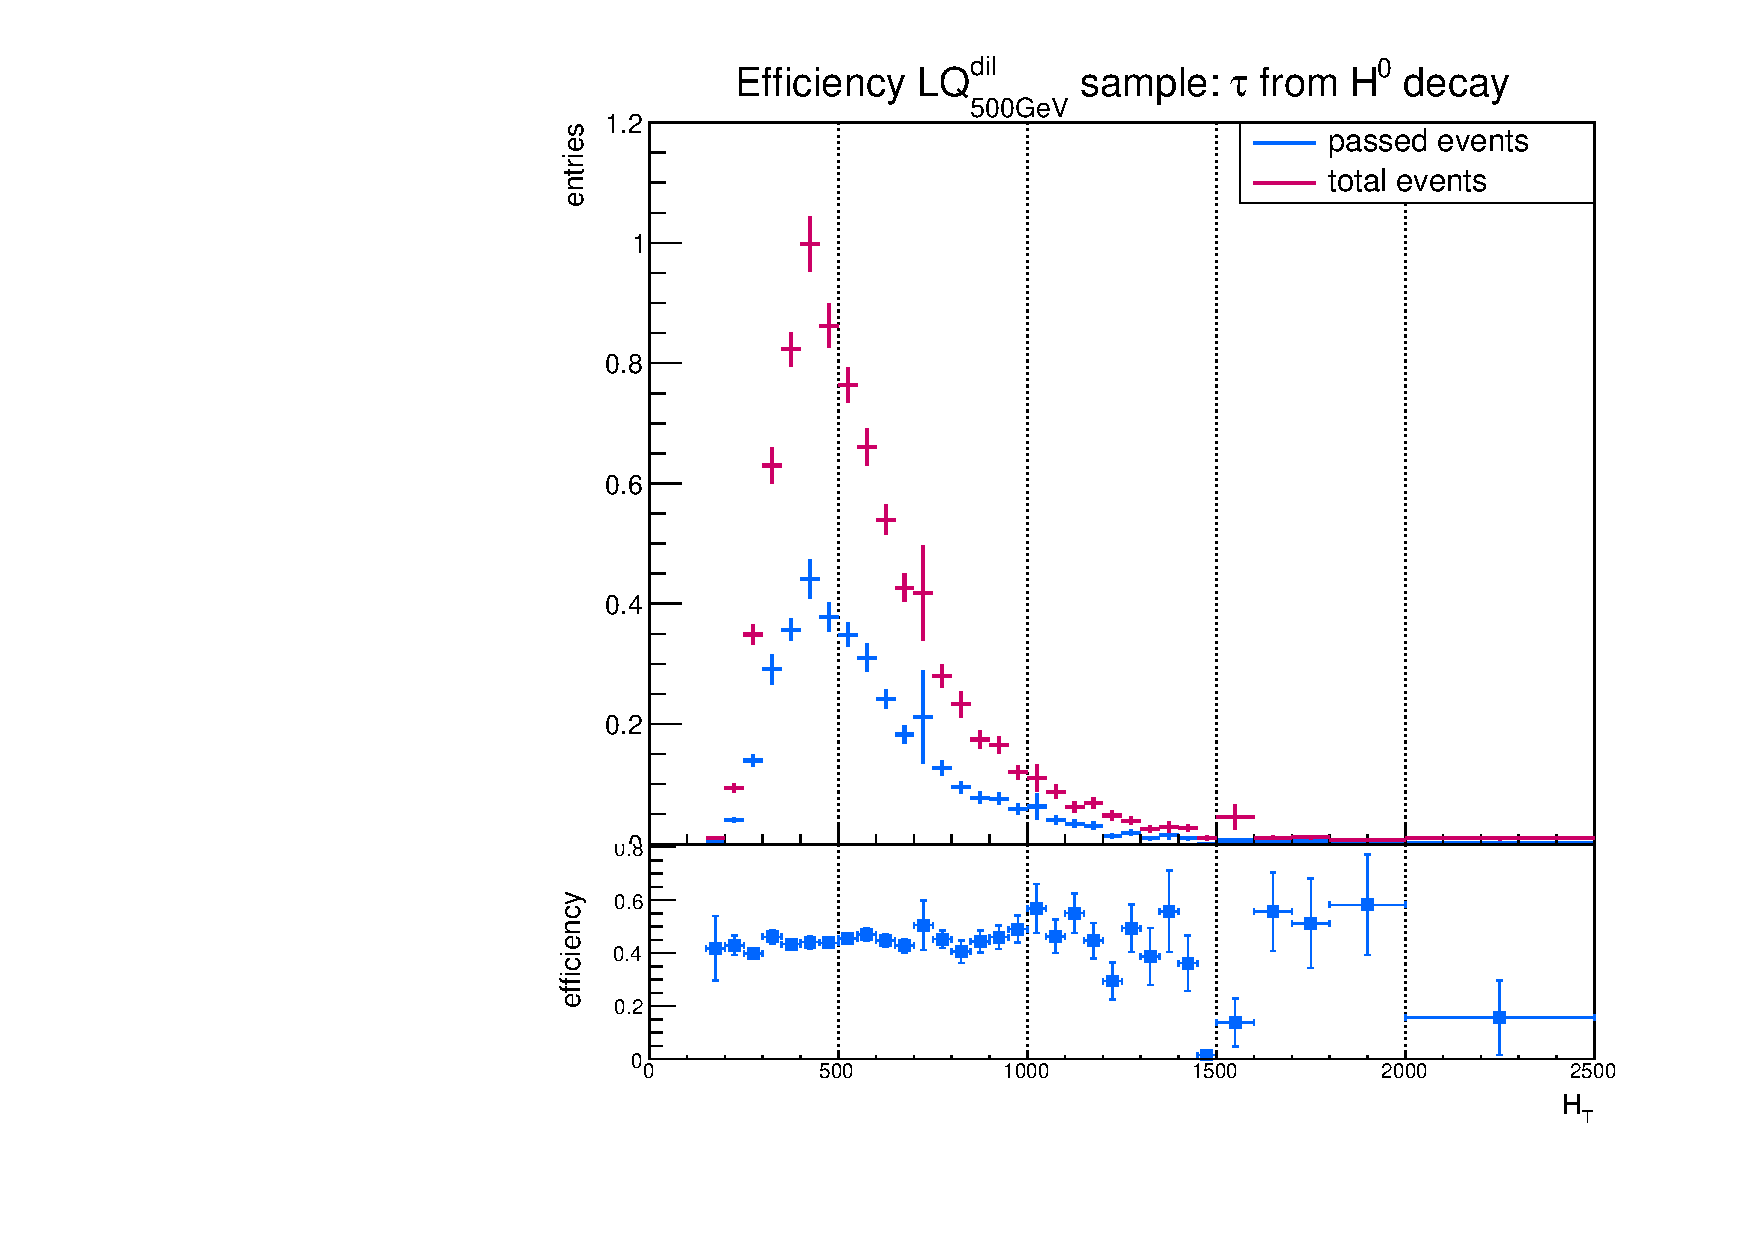
\includegraphics[width=\textwidth]{figures/plots/ttH/Divided_fromHHT.pdf}
                \subcaption{Efficiency of taus originating from Higgs bosons of depending on $H_{T}$ for the Higgs events.}
                \label{Divided:fromH:HT}
                \end{subfigure}
                %
                \begin{subfigure}[t]{0.49\textwidth}
                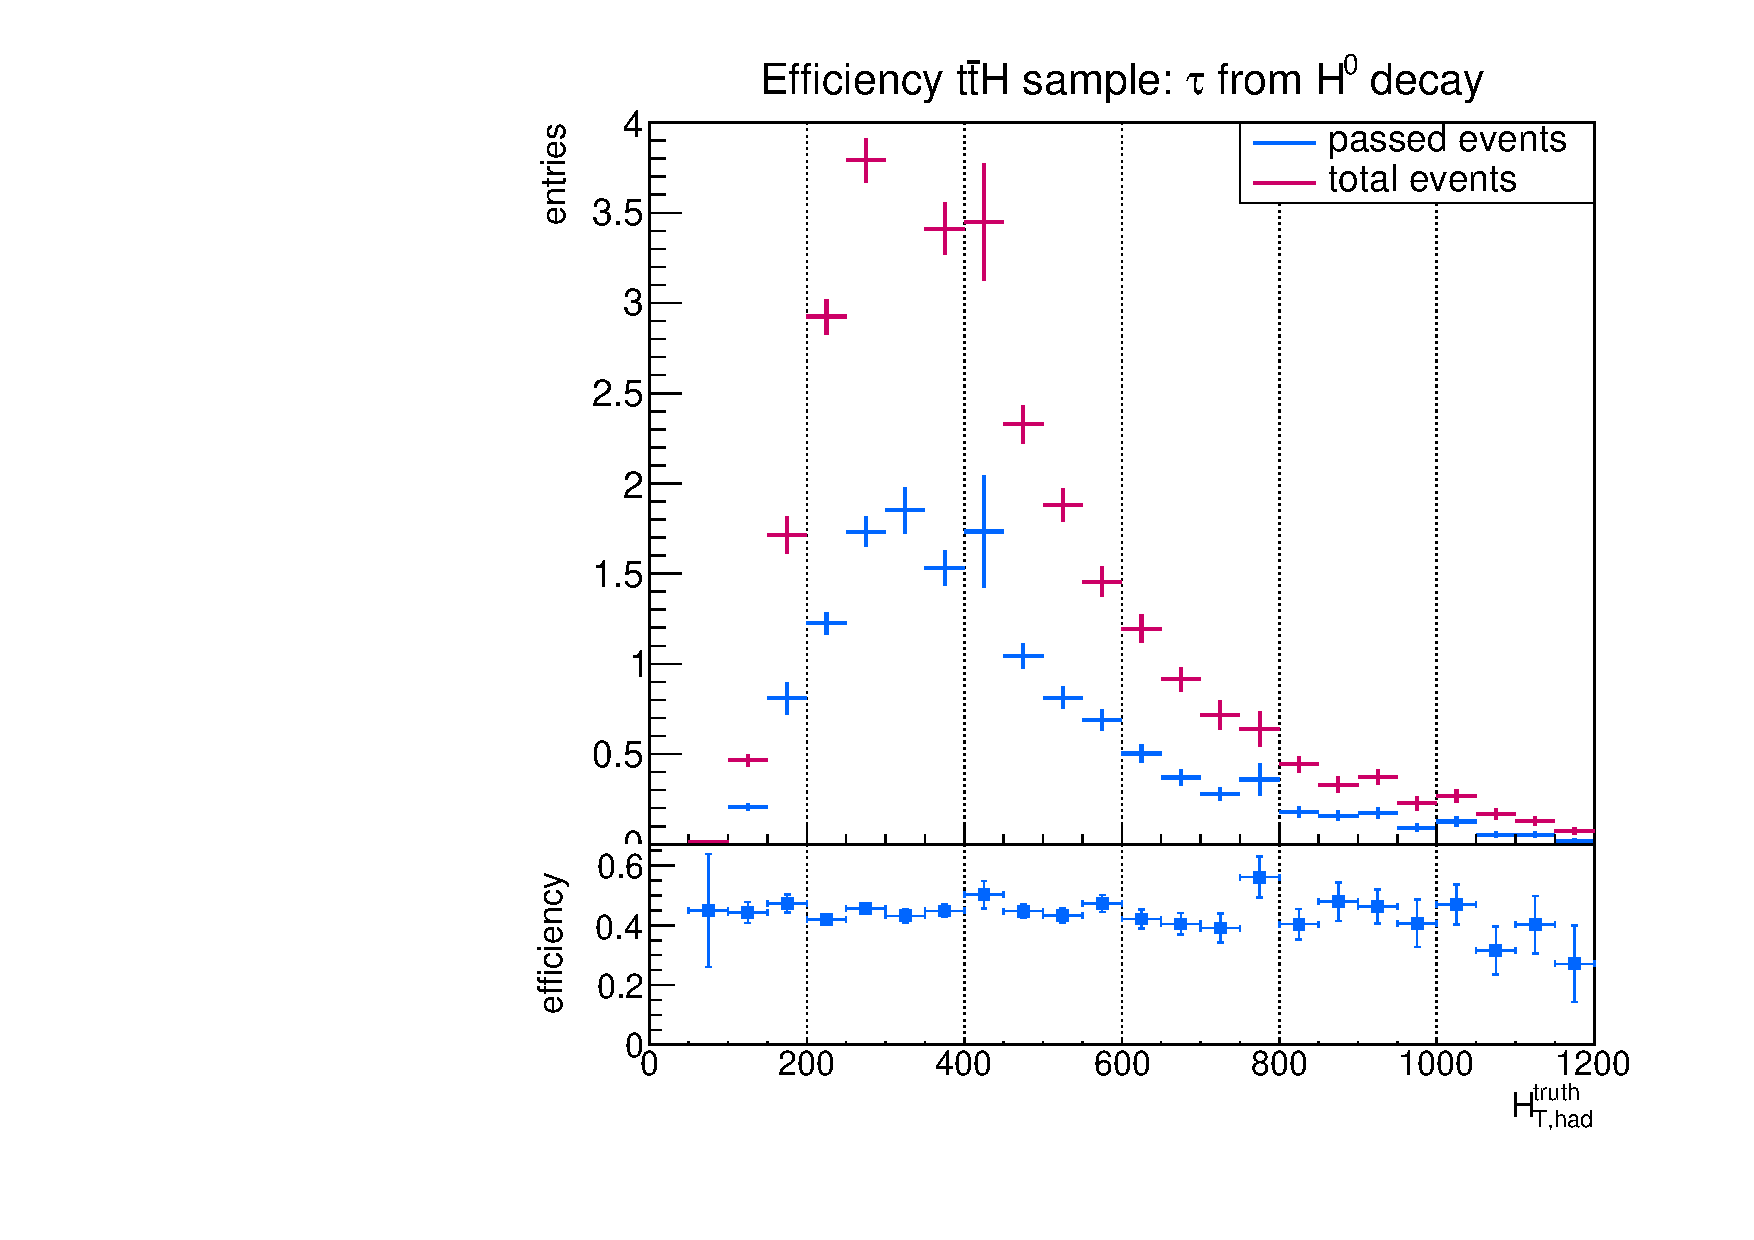
\includegraphics[width=\textwidth]{figures/plots/ttH/Divided_fromHHThad.pdf}
                \subcaption{Efficiency of taus originating from Higgs bosons of depending on $H_{T,\text{had}}$ for the Higgs events.}
                \label{Divided:fromH:HThad}
                \end{subfigure}
\caption[Efficiency of taus originating from Higgs bosons for events from $t\bar{t}H$ sample.]{Efficiency of taus originating from Higgs bosons depending on $H_{T}$ (a) and $H_{T,\text{had}}$ (b)for events from $t\bar{t}H$ sample.}
\label{Divided:fromH:HTgedöns}
\end{figure}
%
%HT und HThad
In figure \ref{Divided:fromH:HTgedöns} the sum of the transverse momenta are shown against the efficiency in case of taus generated by $H^0$. Adding up the electrons' and muons' transverse momentum (see \ref{Divided:fromH:HT}) to the sum of the jets' transverse momentum (see \ref{Divided:fromH:HThad}) influences the number of elements and expands the spectrum, but influences not the shape of the efficiency depicted in the ratio plot. Only slight changes in efficiency is visible apart from the constant efficiency curve in the ratio plot for the variable $H_T$. The difference of the variables regarding electrons and muons adds one remarkable minimum to the efficiency depending on $H_T$ at $\SI{1.45}{\tera\electronvolt}$ to the efficiency dependence, which can be local lack of enough statistcs.\newline
%ST and STlep
\begin{figure}
  \centering
                \begin{subfigure}[t]{0.49\textwidth}
                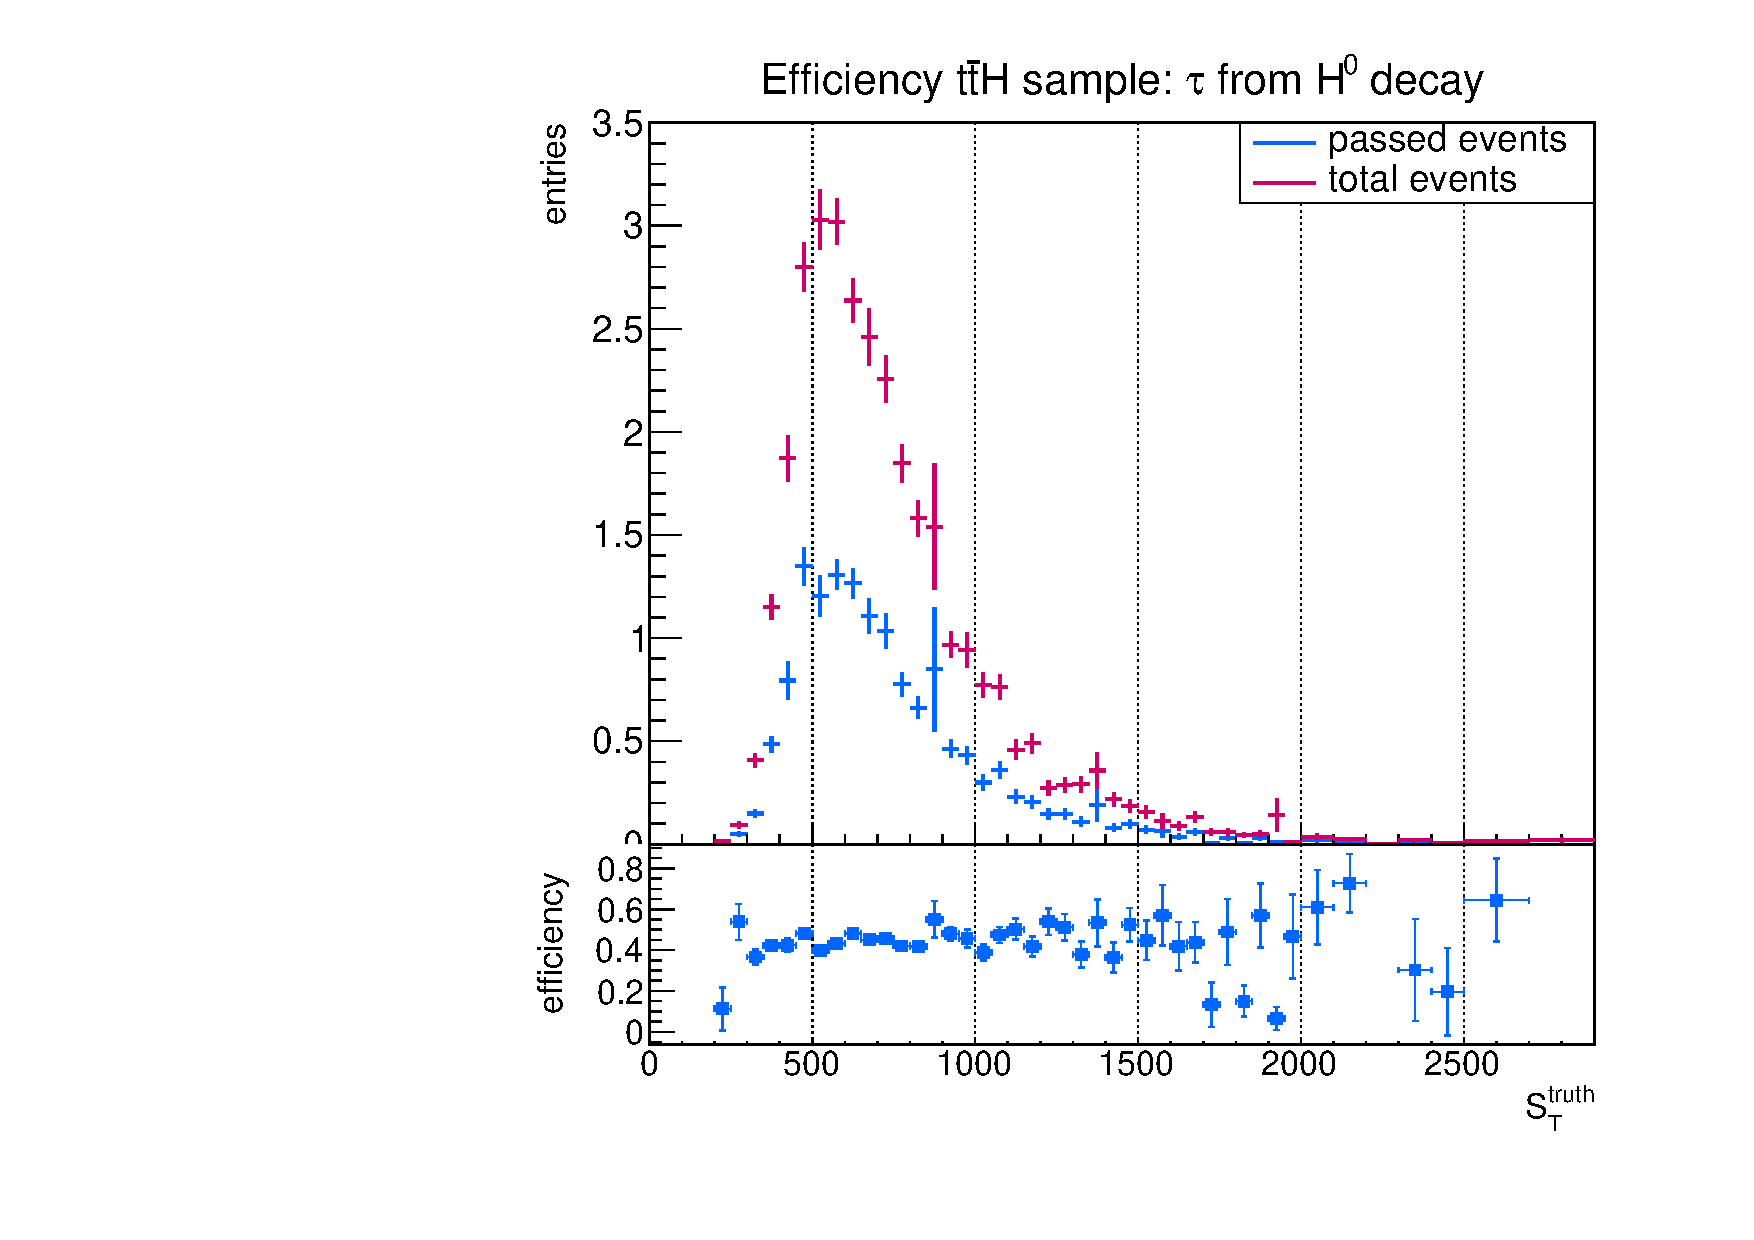
\includegraphics[width=\textwidth]{figures/plots/ttH/Divided_fromHST.pdf}
                \subcaption{Efficiency of taus originating from Higgs bosons of depending on $S_{T}$ for the Higgs events.}
                \label{Divided:fromH:ST}
                \end{subfigure}
                %
                \begin{subfigure}[t]{0.49\textwidth}
                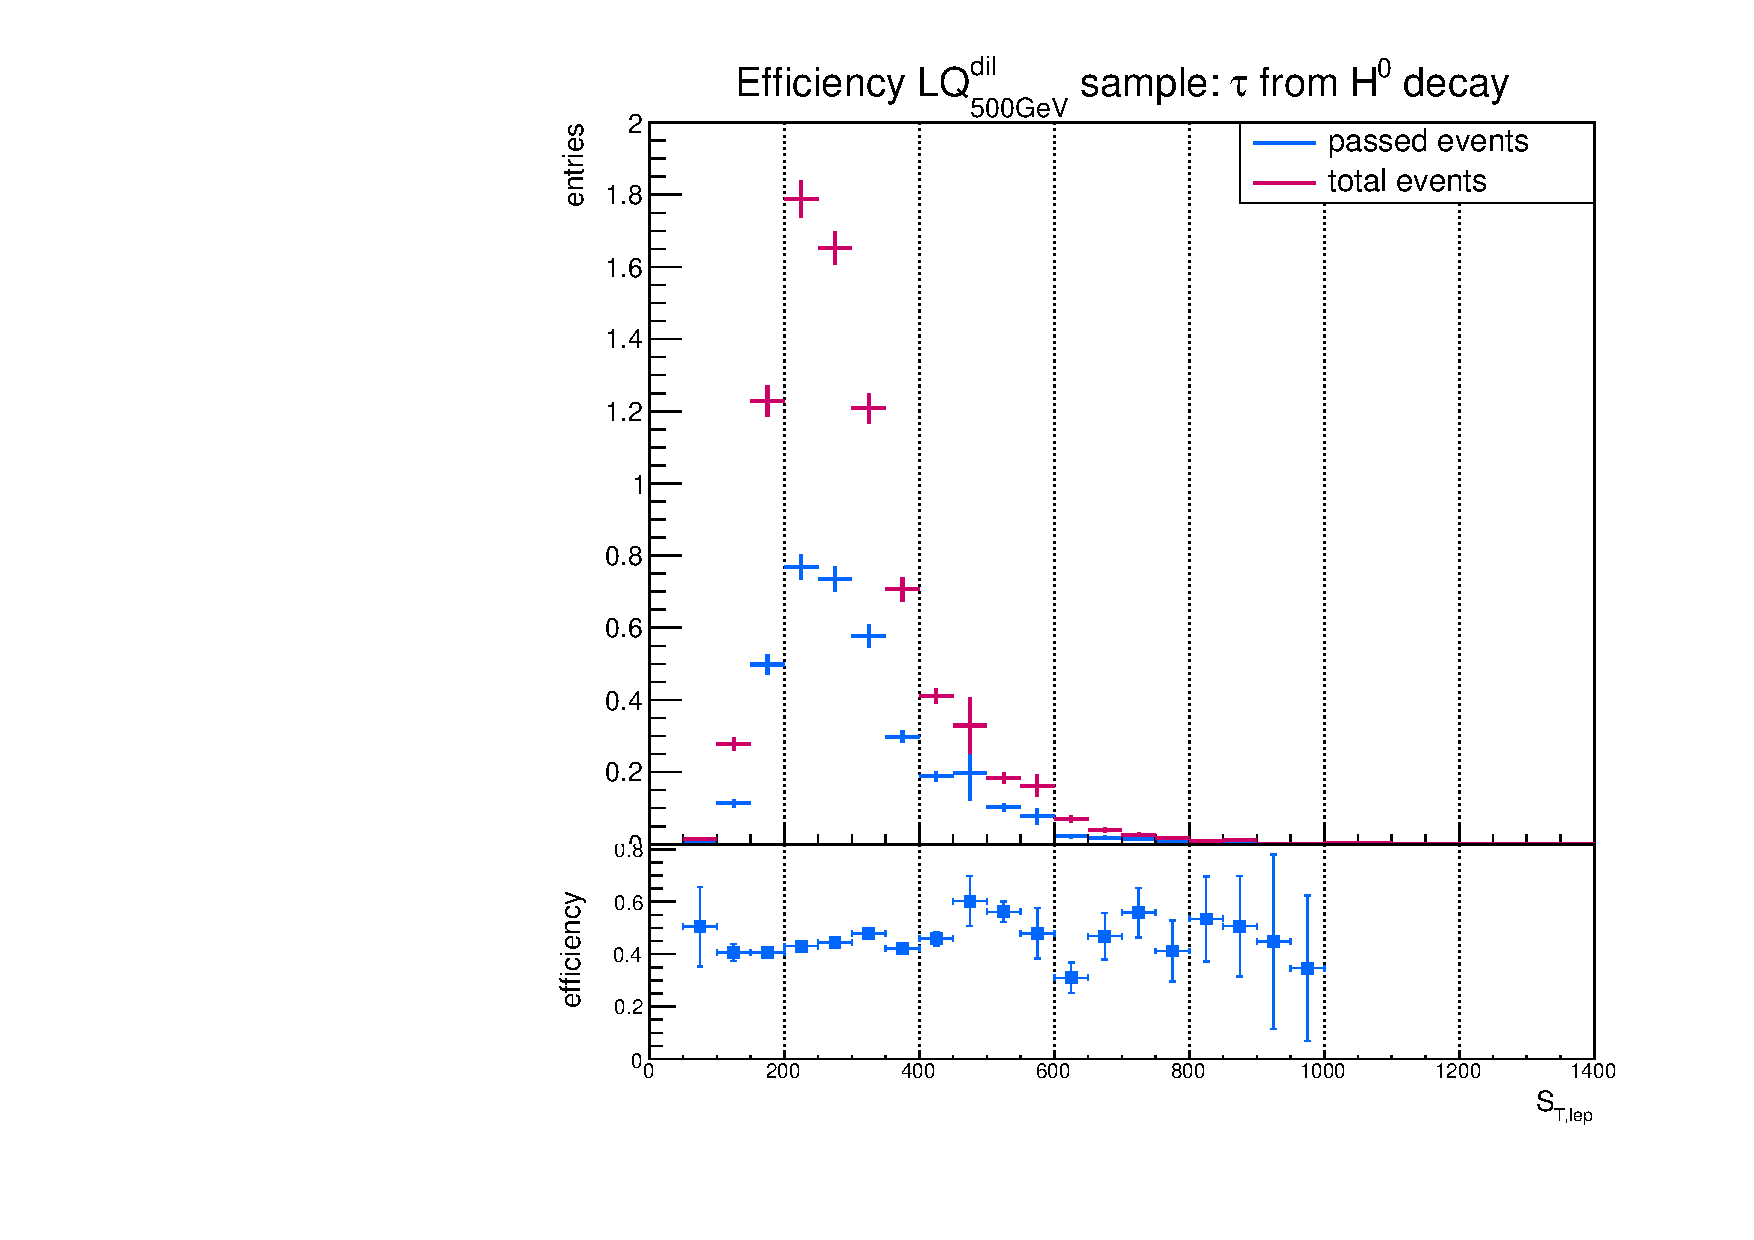
\includegraphics[width=\textwidth]{figures/plots/ttH/Divided_fromHSTlep.pdf}
                \subcaption{Efficiency of taus originating from Higgs bosons of depending on $S_{T,\text{lep}}$ for the Higgs events.}
                \label{Divided:fromH:STlep}
                \end{subfigure}
\caption[Efficiency of taus originating from Higgs bosons for events from $t\bar{t}H$ sample.]{Efficiency of taus originating from Higgs bosons depending on $S_{T}$ (a) and $S_{T,\text{lep}}$ (b) for events from $t\bar{t}H$ sample.}
\label{Divided:fromH:STgedöns}
\end{figure}
%
The sum of all considered objects in $S_T$ or the subset $S_{T,\text{lep}}$ are depicted in figure \ref{Divided:fromH:ST} and \ref{Divided:fromH:STlep} respectively. Efficiency variations over the whole momentum range in $S_T$ are caused mainly by hadronic tau multiplicity and transverse momenta, because $H_T$ and $H_{T,\text{had}}$ does not contain hadronic taus. This conclusion can be drawn from stronger variations in the $S_{T,\text{lep}}$ distribution (see fig. \ref{Divided:fromH:STlep}).\newline  
%njets
The efficiency dependence on the number of jets shows very low efficiency of $\SI{5}{\percent}$ for taus originating from Higgs bosons with 2 jets, while with 3 jets the efficiency increases significantly and its further trend is continuously. The efficiency graph is shown in figure \ref{Divided:fromH:njets}.\newline
%
\begin{figure}
  \centering
                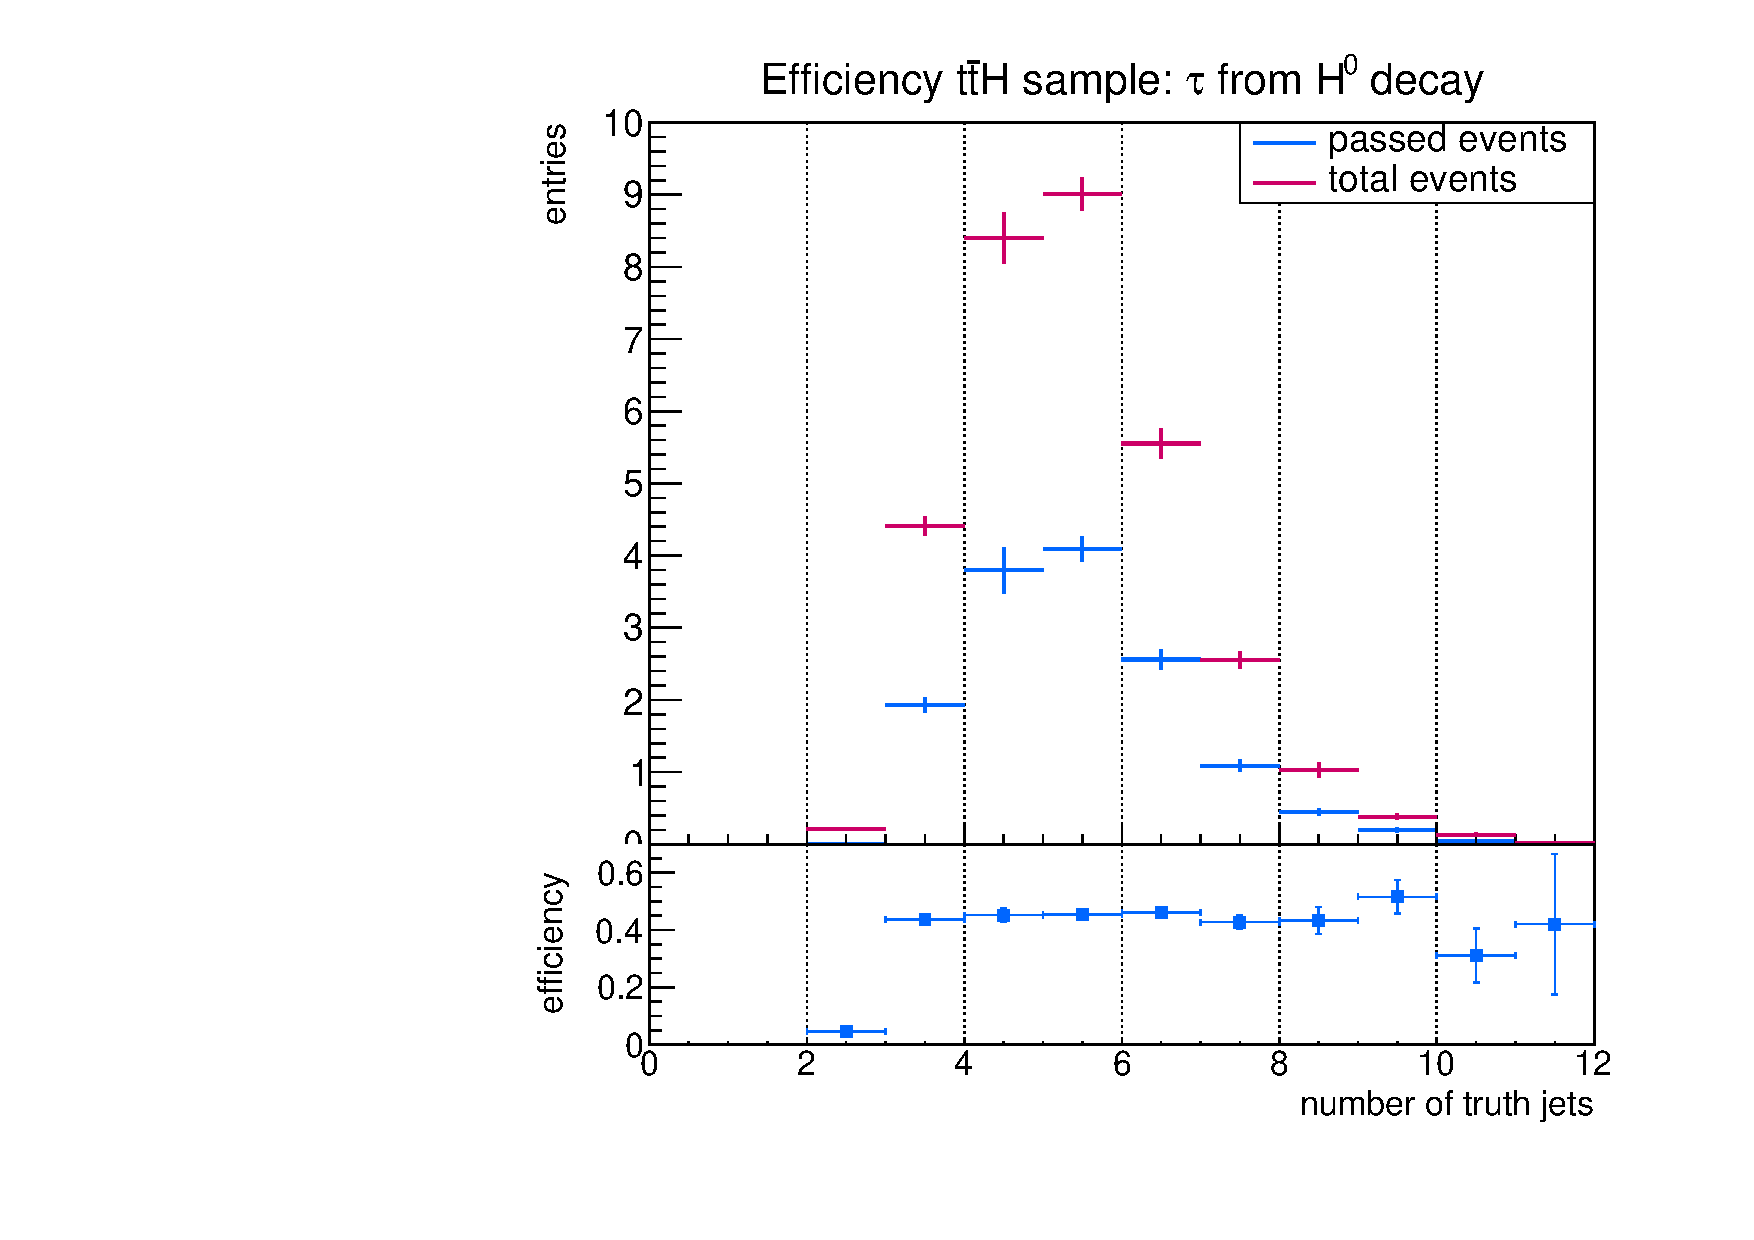
\includegraphics[width=0.5\textwidth]{figures/plots/ttH/Divided_fromHnjets.pdf}
\caption[Efficiency of taus originating from Higgs bosons depending on the number of jets.]{Efficiency of taus originating from Higgs bosons depending on the number of jets.}
\label{Divided:fromH:njets}
\end{figure}
%
%dR min/max Gedöns fromH
Decay characteristics will influence the separation of different objects involved in the event selection. Therefore the minimum and maximum separation $\Delta R$ is studied between taus and leptons, taus and jets as well as taus and b-jets. This is done for taus originated from Higgs bosons.\par
Figure \ref{dR:fromH:taulepton} shows the minimum and maximum separation between taus and light leptons (electrons and muons) for the origin candidate $H^0$. Almost no efficiency dependence for the minimum separation can be detected , besides the low efficiency at $\Delta R<0.5$ which results from overlap removal between these objects. The maximum separation between taus and light leptons in contrast show fluctuations in the separation range $2.4<\Delta R<3.0$. \newline
%
\begin{figure}
  \centering
                \begin{subfigure}[t]{0.49\textwidth}
                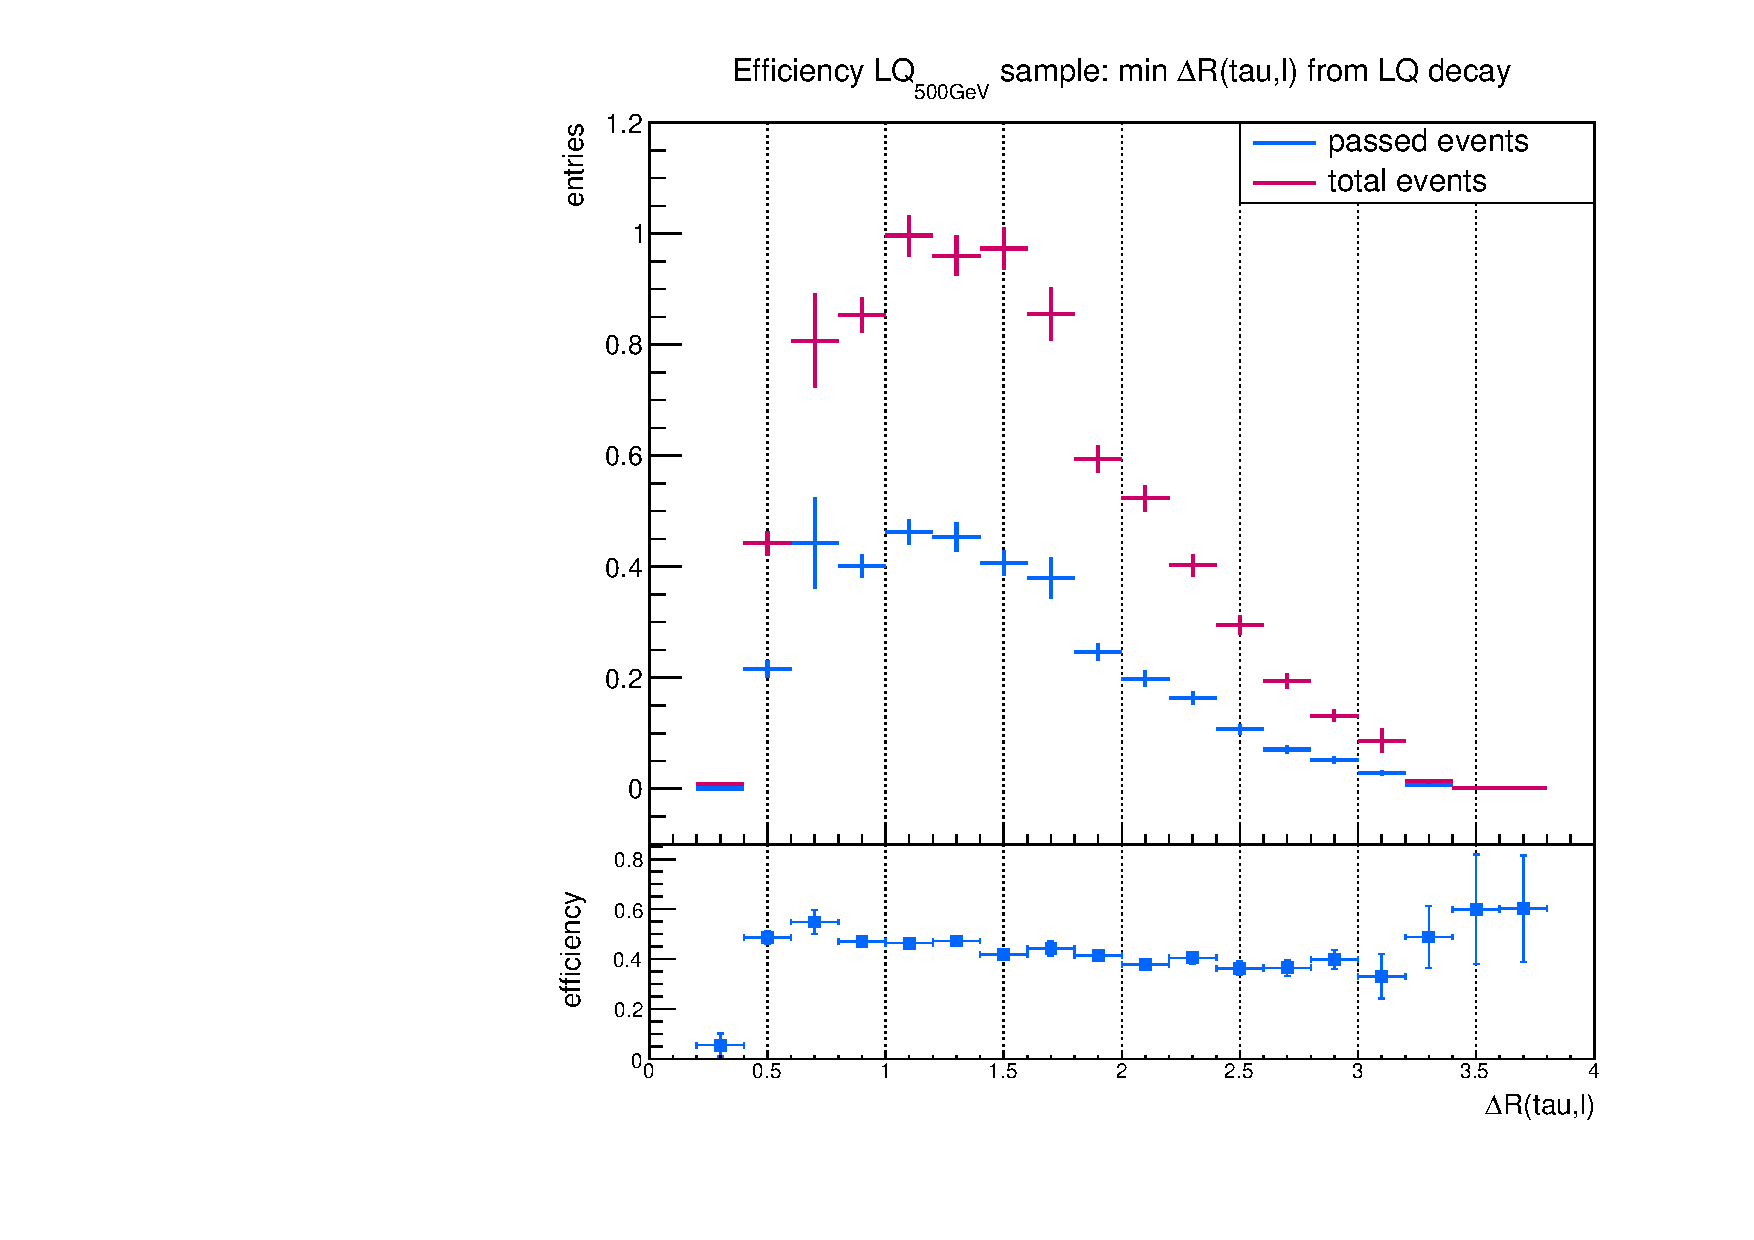
\includegraphics[width=\textwidth]{figures/plots/ttH/Divided_fromH_mindR_taulepton.pdf}
                \subcaption{Minimum separation between taus originating from the Higgs events and leptons.}
                \label{dR:fromH:taulepton:min}
                \end{subfigure}
                 %
                \begin{subfigure}[t]{0.49\textwidth}
                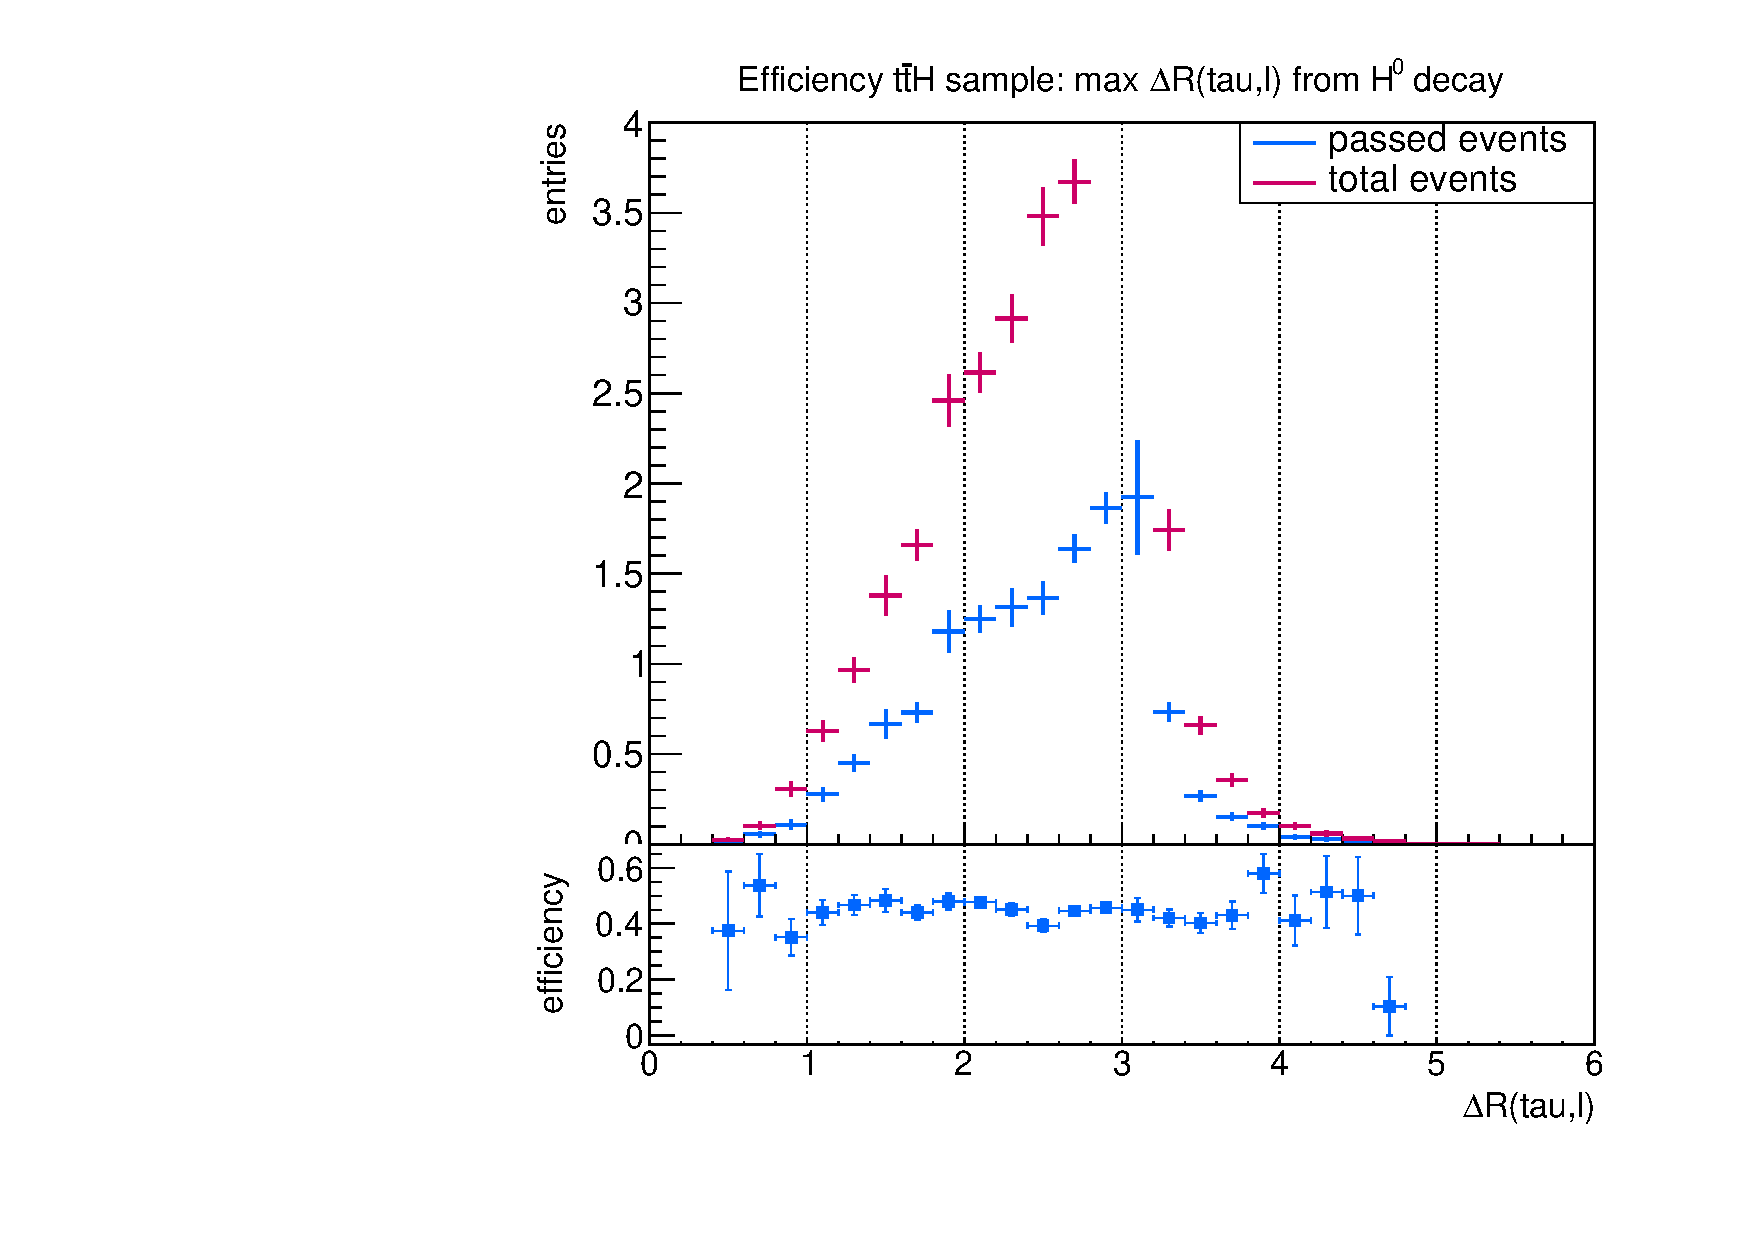
\includegraphics[width=\textwidth]{figures/plots/ttH/Divided_maxdR_fromH_taulepton.pdf}
                \subcaption{Maximum separation between taus originating from the Higgs events and leptons.}
                \label{dR:fromH:taulepton:max}
                \end{subfigure}
\caption[Efficiency of taus originating from Higgs bosons for the separation between taus and leptons.]{Efficiency of taus originating from Higgs bosons for the minimum and maximum separation between taus and leptons (electrons and muons).}
\label{dR:fromH:taulepton}
\end{figure}
%
The minimum and maximum separation between taus and jets is presented in figure \ref{dR:fromH:taujets}. For that case of the taus' origin from Higgs they seem to be either well separated explained by peak in number of tau leptons at $\Delta R=3.0$ for the maximum separation (see figure \ref{dR:fromH:taujets:max}). Or there is no separation shown by the abundant entries for $\Delta R<0.5$ in the minimum separation (see fig. \ref{dR:fromH:taujets:min}), which become the main fake rate contributors for the category jets. High efficiency dependence is shown from the maximum separation in the range of less than $2.0$.\newline
%
\begin{figure}
  \centering
                \begin{subfigure}[t]{0.49\textwidth}
                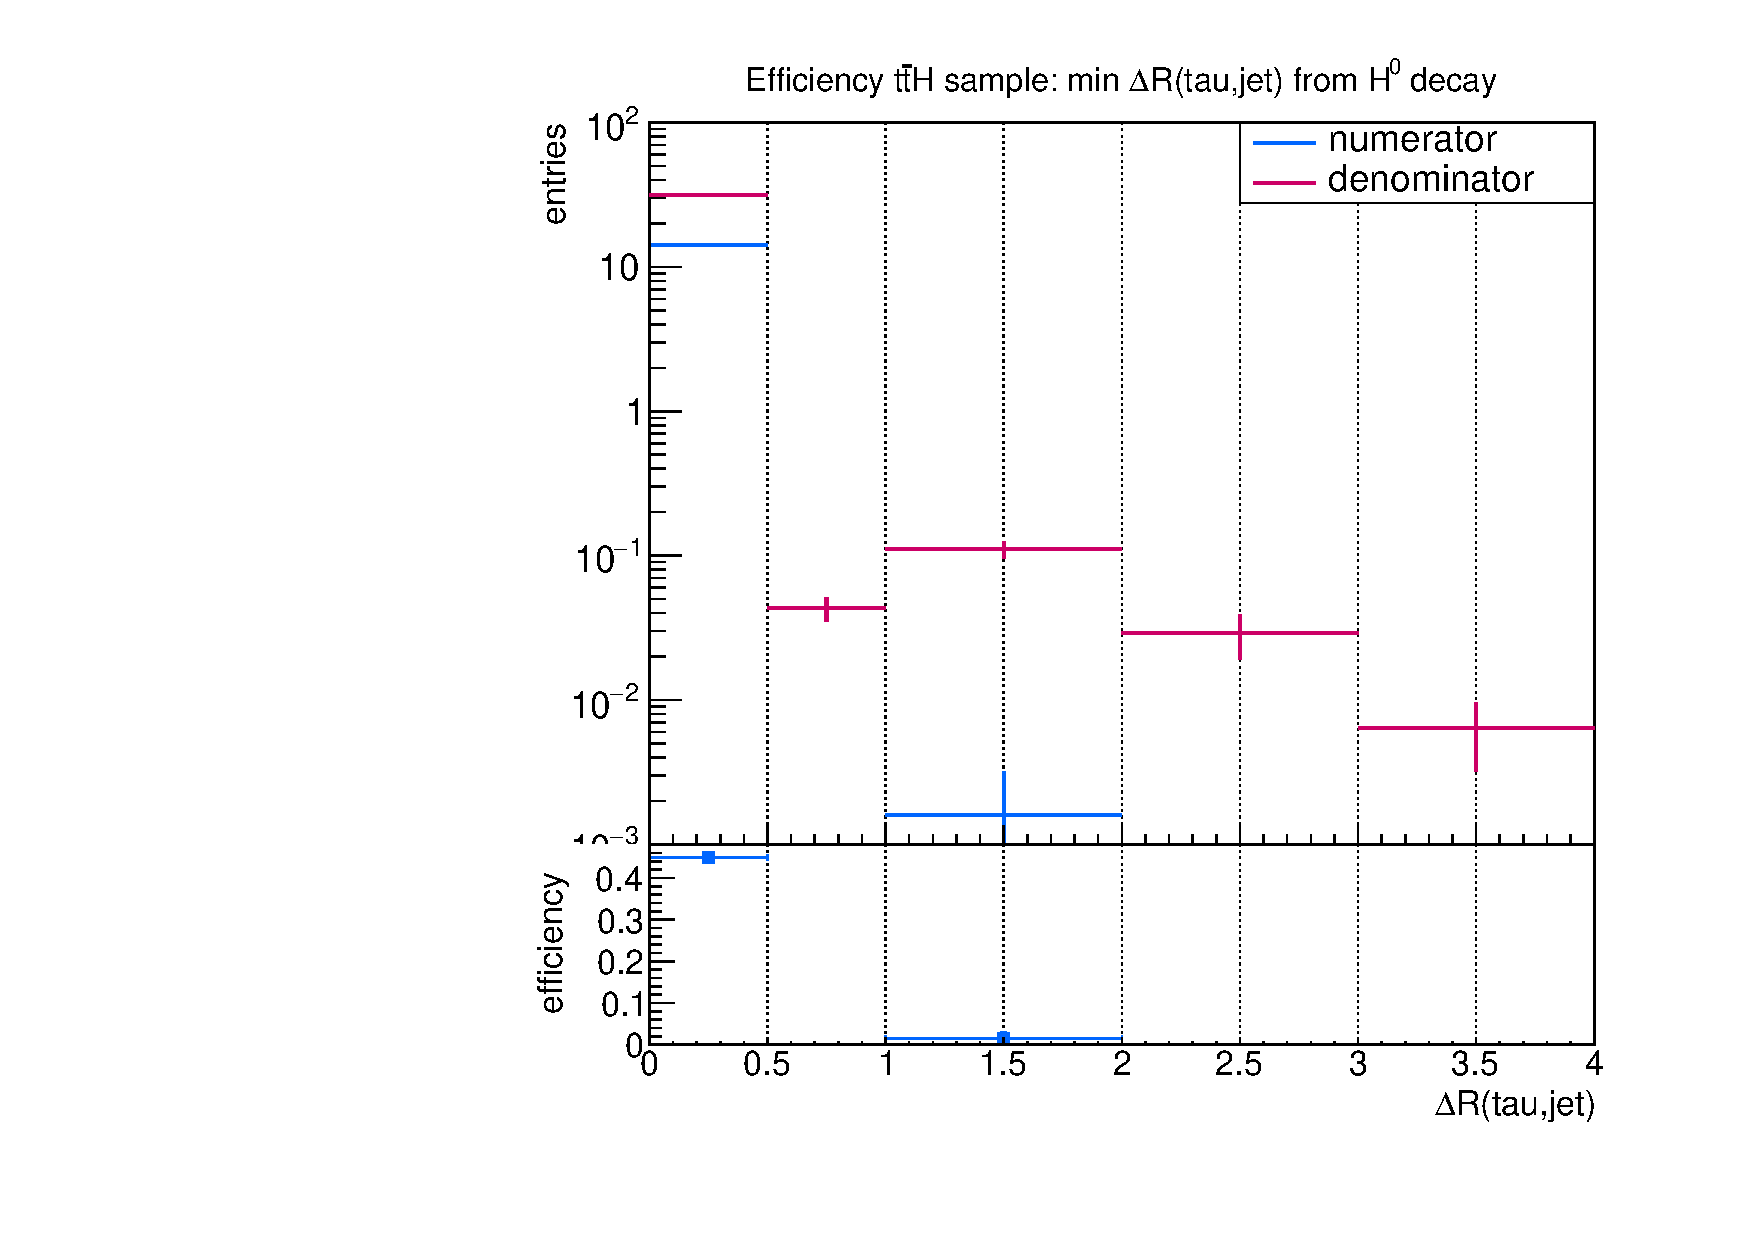
\includegraphics[width=\textwidth]{figures/plots/ttH/Divided_fromH_mindR_taujet.pdf}
                \subcaption{Minimum separation between taus originating from the Higgs events and jets.}
                \label{dR:fromH:taujets:min}
                \end{subfigure}
                 %
                \begin{subfigure}[t]{0.49\textwidth}
                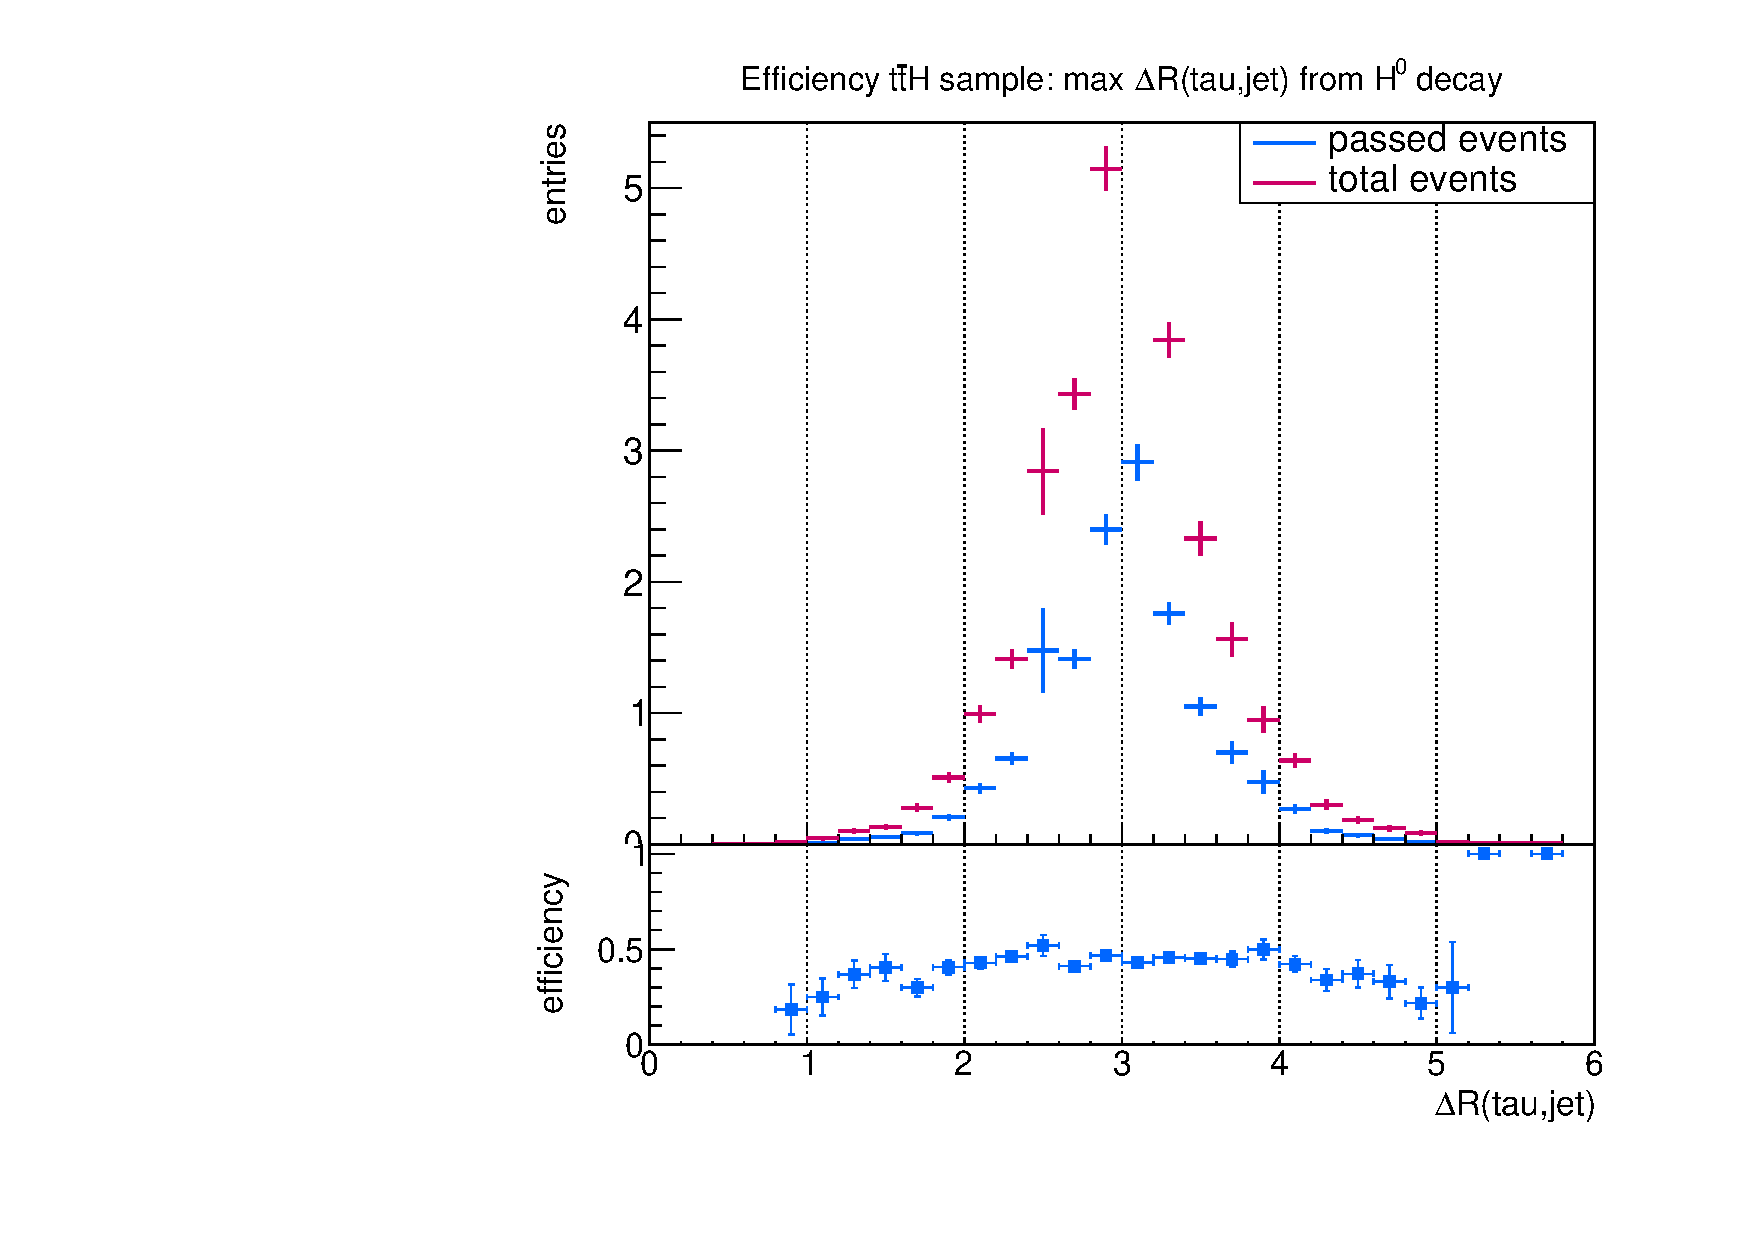
\includegraphics[width=\textwidth]{figures/plots/ttH/Divided_maxdR_fromH_taujet.pdf}
                \subcaption{Maximum separation between taus originating from the Higgs events and jets.}
                \label{dR:fromH:taujets:max}
                \end{subfigure}
\caption[Efficiency of taus originating from Higgs bosons for the separation between taus and jets.]{Efficiency of taus originating from Higgs bosons for the minimum and maximum separation between taus and jets.}
\label{dR:fromH:taujets}
\end{figure}
%
The maximum separation between taus and b-jets shows a slightly shifted peak at $\Delta R=2.8$ compared to the jet separation (see \ref{dR:fromH:taubjets:max}), but the efficiency dependence is very similar to the jets separation. This is valid for taus coming from $H^0$. The minimum separation between taus and b-jets show large changes compared to all jet flavors (see \ref{dR:fromH:taubjets:max}). The minimum separation is extended over a full separation range up to $\Delta R=4.5$ and has significantly less efficiency close to zero for small separations.
%
\begin{figure}
  \centering
                \begin{subfigure}[t]{0.49\textwidth}
                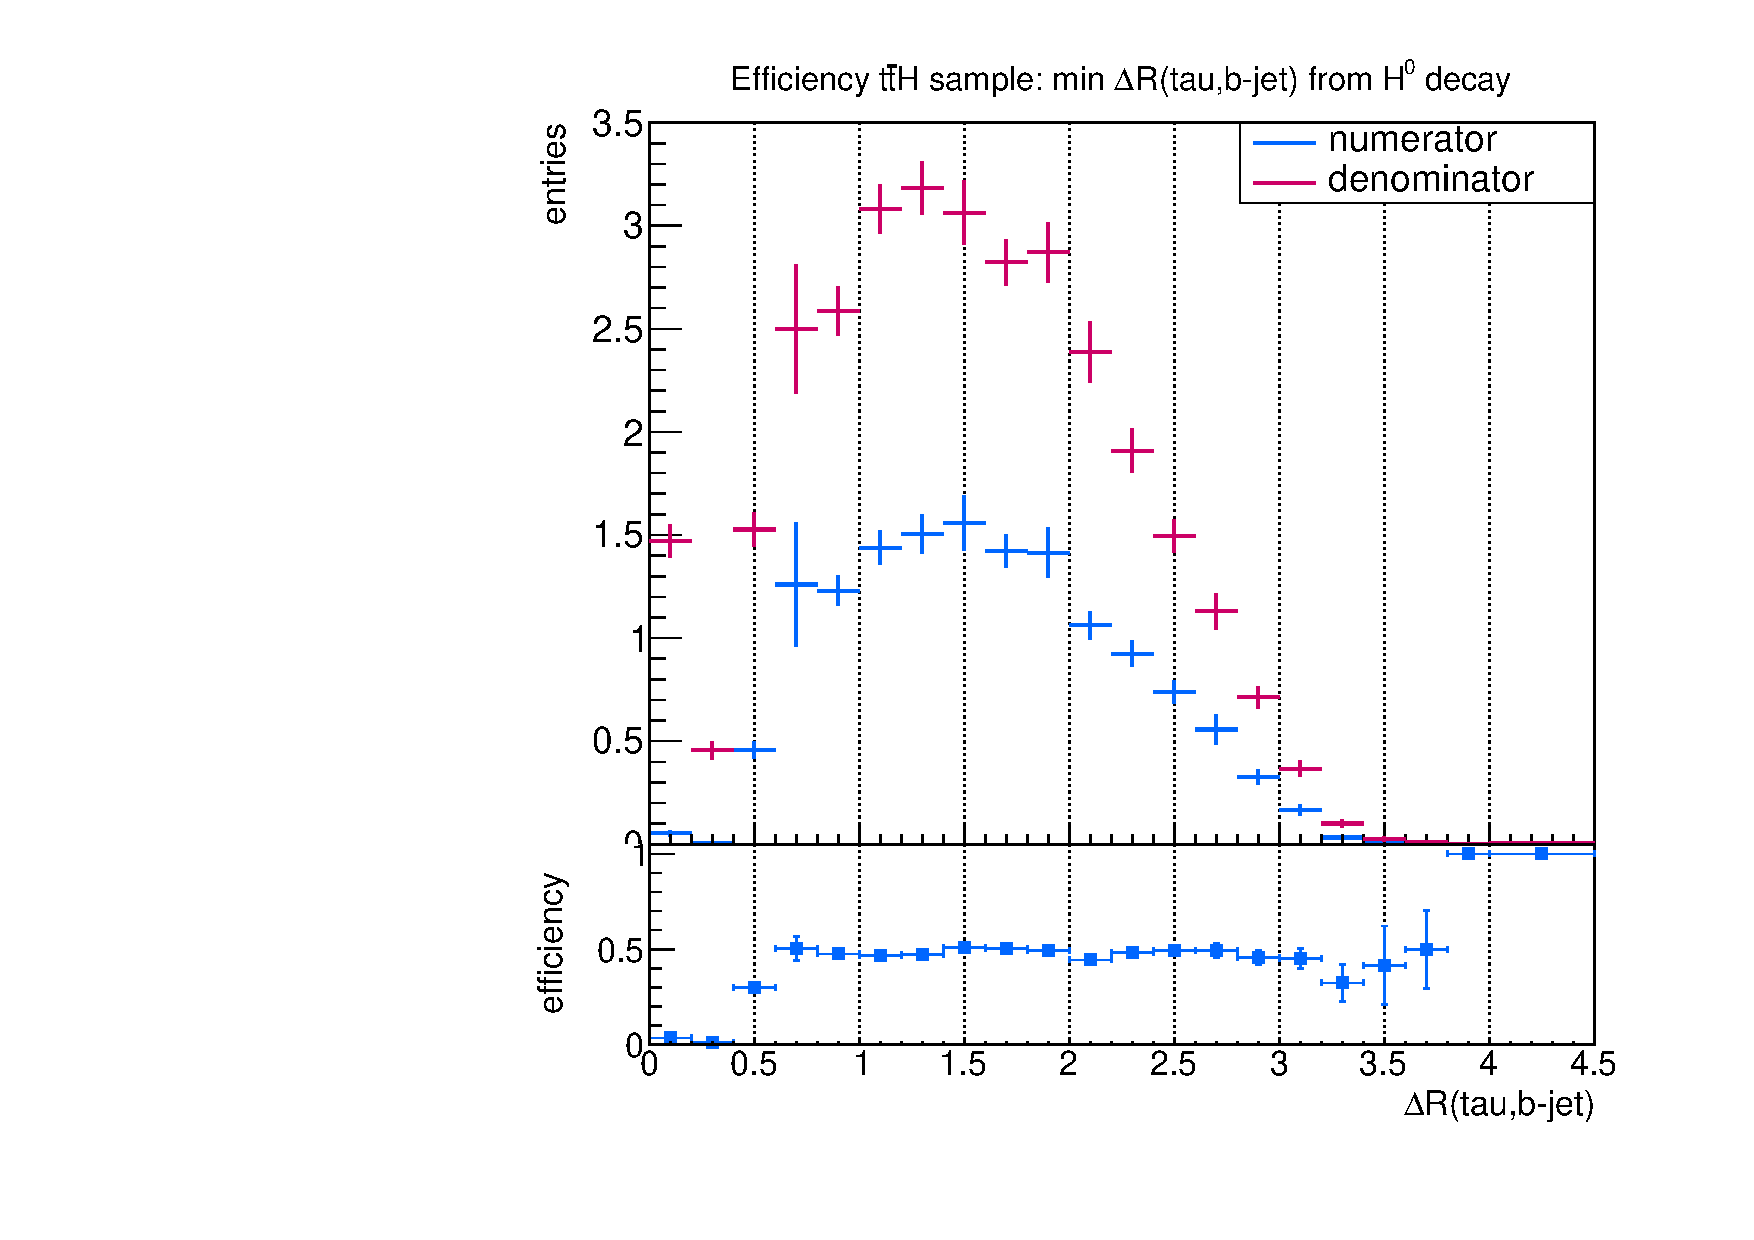
\includegraphics[width=\textwidth]{figures/plots/ttH/Divided_mindR_fromH_taubjet.pdf}
                \subcaption{Minimum separation between taus originating from the Higgs events and b-jets.}
                \label{dR:fromH:taubjets:min}
                \end{subfigure}
                 %
                \begin{subfigure}[t]{0.49\textwidth}
                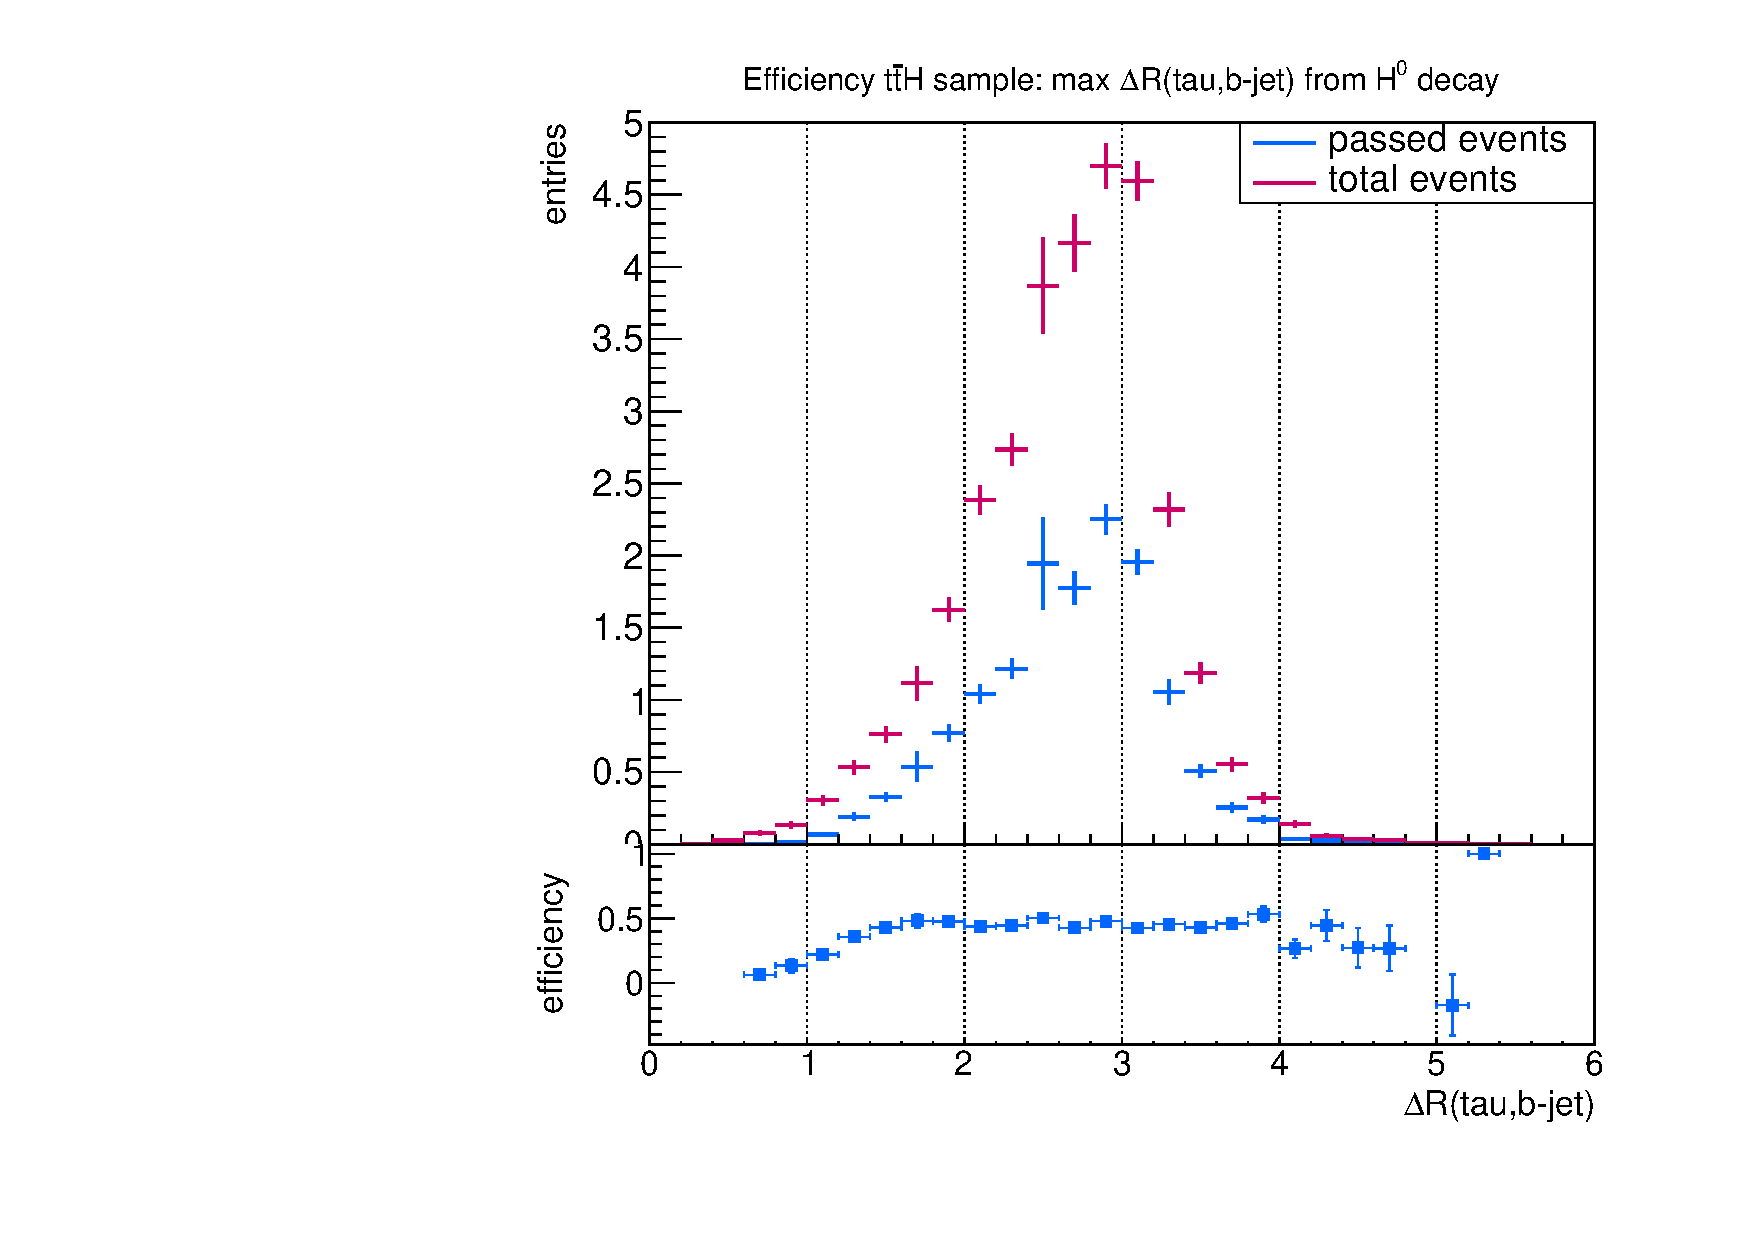
\includegraphics[width=\textwidth]{figures/plots/ttH/Divided_maxdR_fromH_taubjet.pdf}
                \subcaption{Maximum separation between taus originating from the Higgs events and b-jets.}
                \label{dR:fromH:taubjets:max}
                \end{subfigure}
\caption[Efficiency of taus originating from Higgs bosons for the separation between taus and b-jets.]{Efficiency of taus originating from Higgs bosons for the minimum and maximum separation between taus and b-jets.}
\label{dR:fromH:taubjets}
\end{figure}
%
%%%%%%%%%%%%%%%%%%%%%%%%%%%%%%%%%%%%%%%%%%%%%%%%%%%%%%%%%%%%%%%%%%%%%%%%%%%%%%%%%%%%%%%%%%%%%%%%%%%%%%%%%%%%%%%%%%%%%%%%%%%%%%%%%%%%%%%%
%%%%%%%%%%%%%%%%%%%%%%%%%%%%%%%%%%%%%%%%%%%%%%%%%%%%%%%%%%%%%%%%%%%%%%%%%%%%%%%%%%%%%%%%%%%%%%%%%%%%%%%%%%%%%%%%%%%%%%%%%%%%%%%%%%%%%%%%
%%%%%%%%%%%%%%%%%%%%%%%%%%%%%%%%%%%%%%%%%%%%%%%%%%%%%%%%%%%%%%%%%%%%%%%%%%%%%%%%%%%%%%%%%%%%%%%%%%%%%%%%%%%%%%%%%%%%%%%%%%%%%%%%%%%%%%%%
%%%%%%%%%%%%%%%%%%%%%%%%%%%%%%%%%%%%%%%%%%%%%%%%%%%%%%%%%%%%%%%%%%%%%%%%%%%%%%%%%%%%%%%%%%%%%%%%%%%%%%%%%%%%%%%%%%%%%%%%%%%%%%%%%%%%%%%%
\subsection{Taus reconstruction efficiency in signal samples}\label{signaleff}
The efficiencies for the leptoquark signal samples with their two mass points are summarized in table \ref{LQEffTable} following the example of the background efficiencies in table \ref{ttbarttHEffTable}. The uncertainty is derived from the binomial error of the efficiency after eq. (\ref{binomialerror}). The efficiency definition is the same as for the background samples (see eq. (\ref{effeq})) with the difference that the category of taus originating from a Higgs boson is replaced by the category of tau leptons originating from leptoquarks.\par
%	
	\begin{sidewaystable}[htbp]
		\centering
                \footnotesize
                \renewcommand{\arraystretch}{1.2}
		\begin{tabular*}{\linewidth}{@{\extracolsep{\fill}}ccccc}
		\hline
		\hline
		 \textbf{sample}  & \multicolumn{2}{c}{\textbf{LQ$_{500\textbf{GeV}}$}}  & \multicolumn{2}{c}{\textbf{LQ$_{1\textbf{TeV}}$}} 
		\\
		\hline
		\multirow{2}{*}{selection}  & reconstructed taus       & total number  & reconstructed taus       & total number 
		\\
                & matched to truth taus & of taus       & matched to truth taus & of taus
                \\
		\hline
		%truth matching for tau      & $1339$            & $2764$      & $1235$        & $2761$
		%\\
		%efficiency                  & \multicolumn{2}{c}{$\SI{48.44\pm 0.95}{\percent}$}    & \multicolumn{2}{c}{$\SI{44.73\pm 0.95}{\percent}$}
		%\\
		%\hline
		%tau originated from W$^{\pm}$, Z$^0$& $36$        & $111$         & $31$          & $149$
		%\\
		%efficiency                  & \multicolumn{2}{c}{$\SI{32.4\pm 4.4}{\percent}$}   & \multicolumn{2}{c}{$\SI{20.8\pm 3.3}{\percent}$}
		%\\
		%\hline
                %tau originated from W$^{\pm}$, Z$^0$ (1-prong)& $26$        & $79$         & $26$          & $110$
		%\\
		%efficiency                  & \multicolumn{2}{c}{$\SI{32.9\pm 5.3}{\percent}$}   & \multicolumn{2}{c}{$\SI{23.6\pm 4.1}{\percent}$}
		%\\
		%\hline
                %tau originated from W$^{\pm}$, Z$^0$ (3-prong)& $10$        & $29$         & $4$          & $32$
		%\\
		%efficiency                  & \multicolumn{2}{c}{$\SI{34.5\pm 8.8}{\percent}$}   & \multicolumn{2}{c}{$\SI{12.5\pm 5.8}{\percent}$}
		%\\
		%\hline
                tau originated from LQ& $905$        & $1764$         & $571$          & $1127$
		\\
		efficiency                  & \multicolumn{2}{c}{$\SI{51.3\pm 1.2}{\percent}$}   & \multicolumn{2}{c}{$\SI{50.7\pm 1.5}{\percent}$}
		\\
		\hline
                tau originated from LQ (1-prong)& $745$        & $1343$         & $160$          & $419$
		\\
		efficiency                  & \multicolumn{2}{c}{$\SI{55.5\pm 1.4}{\percent}$}   & \multicolumn{2}{c}{$\SI{55.0\pm 1.7}{\percent}$}
		\\
		\hline
                tau originated from LQ (3-prong)& $160$        & $419$         & $94$          & $259$
		\\
		efficiency                  & \multicolumn{2}{c}{$\SI{38.2\pm 2.4}{\percent}$}   & \multicolumn{2}{c}{$\SI{36.3\pm 3.0}{\percent}$}
		\\
		%\hline
		%tau from B-mesons           & $1$            & $110$      & $1$            & $107$ 
		%\\
		%efficiency                  & \multicolumn{2}{c}{$\SI{0.91\pm 0.90}{\percent}$}   & \multicolumn{2}{c}{$\SI{0.93\pm 0.93}{\percent}$}
		\\
		%\hline
		%jet faking as tau            & $3452$         & $43922$      & $3728$         & $53495$ 
		%\\
		%efficiency                  & \multicolumn{2}{c}{$\SI{7.86\pm 0.13}{\percent}$}   & \multicolumn{2}{c}{$\SI{6.97\pm 0.11}{\percent}$}
		%\\
		%\hline
		%b-jet faking as tau          & $38$        & $1613$      & $33$         & $1842$ 
		%\\
		%efficiency                  & \multicolumn{2}{c}{$\SI{2.36\pm 0.38}{\percent}$}   & \multicolumn{2}{c}{$\SI{1.79\pm 0.31}{\percent}$}
		%\\
		%\hline
                %not b-jet faking as tau          & $3414$        & $27788$      & $3695$         & $35075$ 
		%\\
		%efficiency                  & \multicolumn{2}{c}{$\SI{12.29\pm 0.20}{\percent}$}   & \multicolumn{2}{c}{$\SI{10.53\pm 0.16}{\percent}$}
		%\\
                %\hline
                %electron faking as tau          & $2$        & $7871$      & $5$         & $8906$ 
		%\\
		%efficiency                  & \multicolumn{2}{c}{$\SI{0.025\pm 0.018}{\percent}$}   & \multicolumn{2}{c}{$\SI{0.056\pm 0.025}{\percent}$}
		%\\
		\hline
		\hline
		\end{tabular*}
		\caption[Efficiencies for the two LQ samples with $\SI{500}{\giga\electronvolt}$ and $\SI{1}{\tera\electronvolt}$ mass point.]{Efficiencies for different tau lepton categories for the two different LQ Monte Carlo samples with $\SI{500}{\giga\electronvolt}$ and $\SI{1}{\tera\electronvolt}$ mass point. The efficiency is defined as $\epsilon=\frac{\text{\#truth hadronic }\tau\text{ matched to a reconstructed }\tau+Z}{\text{\#truth }\tau\text{ passing the basic selection}+Z}$.}
		\label{LQEffTable}
                \renewcommand{\arraystretch}{1}
                \end{sidewaystable}
%
%Truth match
%The efficiency for reconstructing a hadronic tau, which is matched to a truth tau over the total number of truth taus passing the basic selection is $\SI{48.44\pm 0.95}{\percent}$ and $\SI{44.73\pm 0.95}{\percent}$ for the $\SI{500}{\giga\electronvolt}$ and $\SI{1}{\tera\electronvolt}$ mass point LQ sample respectively. These higher efficiencies compared to the background samples are caused by the existence of more real taus due to the LQ decay. This can be seen also at the momentum spectrum in figure \ref{DividedTau:signal}, where the truth tau's transverse momentum is drawn against the efficiency.\par  
%
%\begin{figure}
%  \centering
%                \begin{subfigure}[t]{0.49\textwidth}
%                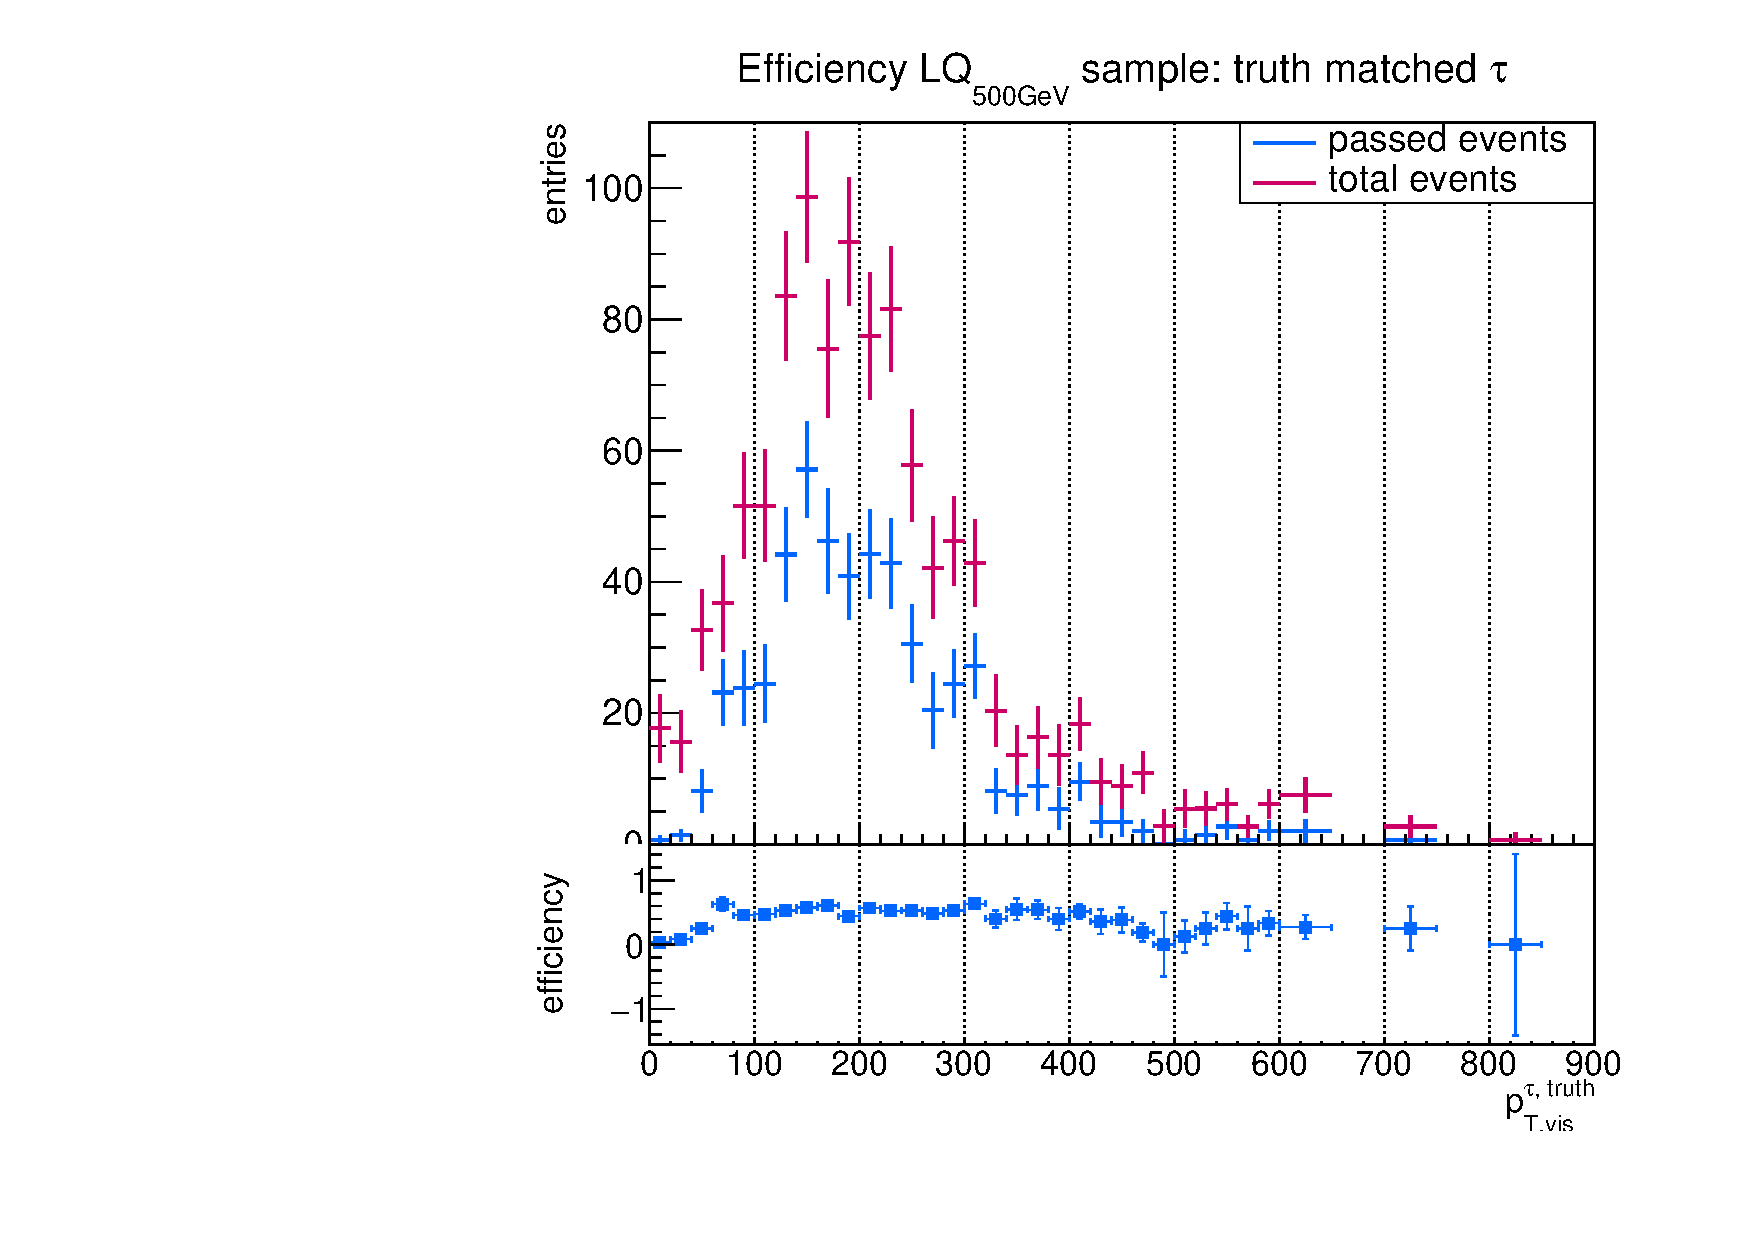
\includegraphics[width=\textwidth]{figures/plots/LQ75/Divided_Tau.pdf}
%                \subcaption{Hadronic tau reconstruction efficiency of $\SI{48.44\pm 0.95}{\percent}$ for the low mass LQ signal events.}
%                \label{DividedTau:signal:LQ75}
%                \end{subfigure}
%                %
%                \begin{subfigure}[t]{0.49\textwidth}
%                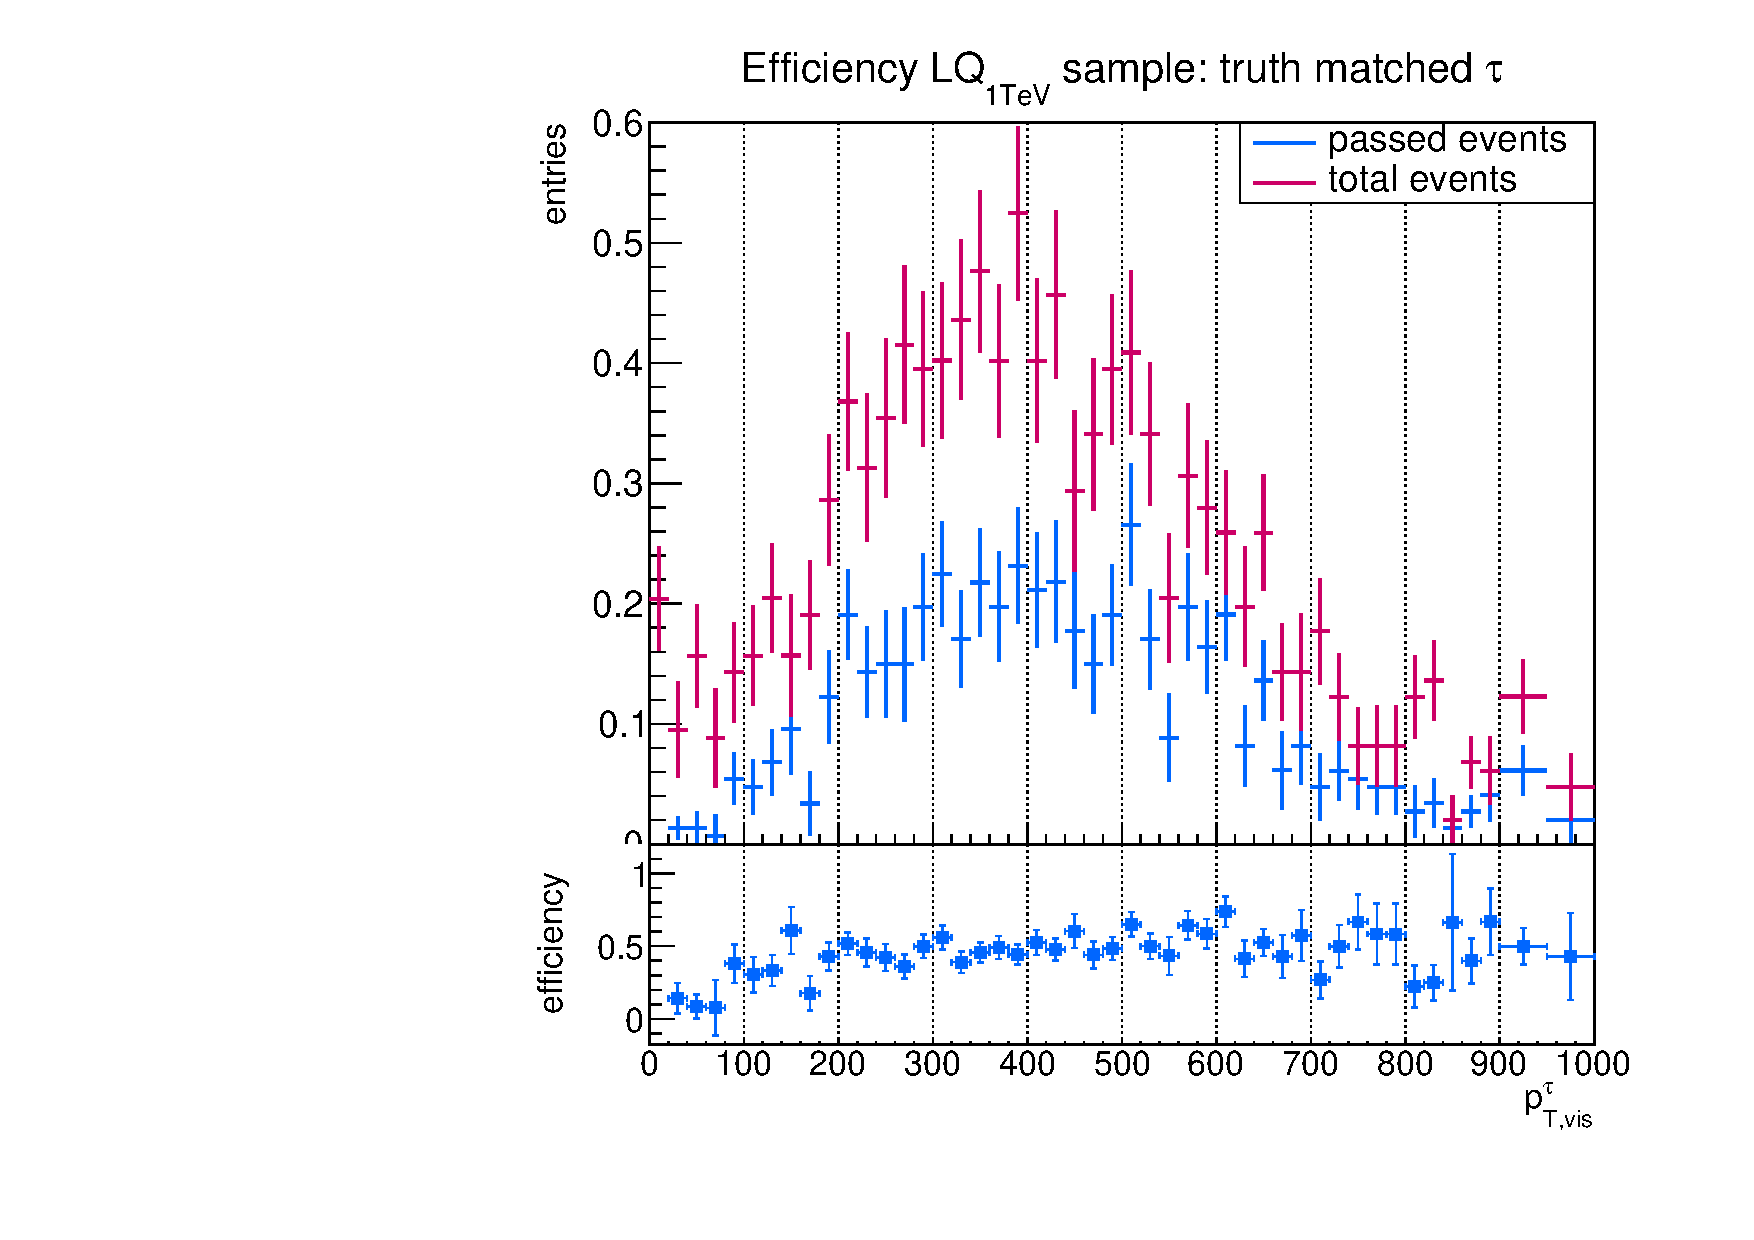
\includegraphics[width=\textwidth]{figures/plots/LQ76/Divided_Tau.pdf}
%                \subcaption{Hadronic tau reconstruction efficiency of $\SI{44.73\pm 0.95}{\percent}$ for the high mass LQ signal events.}
%                \label{DividedTau:signal:LQ76}
%                \end{subfigure}
%\caption[Hadronic tau reconstruction efficiency for the signal events.]{Hadronic tau reconstruction efficiency for the signal events. The efficiency is defined as number of reconstructed hadronic taus passing the basic selection and is matched to a truth tau over the number of truth taus passing the basic selection (truth matching tau).}
%\label{DividedTau:signal}
%\end{figure}
%
%B mesons %if eff has dependence on pT of the objects this difference is expected because of different kinematics
%With a mean efficiency value of roughly $\sim\SI{1}{\percent}$ taus originating from B-mesons the rate is as twice as high compared to the two background samples. Nevertheless this is a small contribution compared to other tau sources and more important, because of the low statistics of only one event and the resulting high uncertainty, this sub-category can be neglected in the overall consideration.\par  
%prompt
%The weak gauge bosons remain as tau sources with an efficiency of $\SI{32.4\pm 4.4}{\percent}$ for the LQ$_{500\textbf{GeV}}$ sample. This is comparable with the efficiency in the same sub-category for the Higgs background sample (cf. table \ref{ttbarttHEffTable}). But the higher mass point LQ sample shows a smaller efficiency of $\SI{20.8\pm 3.3}{\percent}$ in that sub-selection. This means that the behavior regarding tau sources from $W^\pm$ and $Z^0$ is comparable in both signal and $t\bar{t}H$ background samples. The efficiency depending on the truth taus' transverse momentum is shown in figure \ref{Dividedprompt:signal:LQ75} and \ref{Dividedprompt:signal:LQ76} for the low and the high LQ mass point respectively. A further sub-selection differentiates between the tau decay into one and three charged particles, which can be seen in figure \ref{Dividedprompt:signal:1prongLQ75} and \ref{Dividedprompt:signal:3prongLQ75} for the low mass point. The $p_{T,\text{vis}}^{\tau,\text{truth}}$ range reaches $\SI{300}{\giga\electronvolt}$ and $\SI{250}{\giga\electronvolt}$ and shows an increasing efficiency with increasing transverse momentum. This effect is known from events from $t\bar{t}H$ sample. The overall efficiency for the 1-prong case is $\SI{32.9\pm 5.3}{\percent}$ and for the 3-prong case is $\SI{34.5\pm 8.8}{\percent}$. For the high mass point the 1-prong and 3-prong decay is shown in figure \ref{Dividedprompt:signal:1prongLQ76} and \ref{Dividedprompt:signal:3prongLQ76} and has efficiencies of $\SI{23.6\pm 4.1}{\percent}$ and $\SI{12.5\pm 5.8}{\percent}$ respectively.
%
%from LQ
Taus originating directly from LQs have an efficiency of $\SI{51.3\pm 1.2}{\percent}$ and $\SI{50.7\pm 1.5}{\percent}$ for the low and high mass point respectively. These to efficiencies are in agreement with each other. The corresponding efficiency plots can be found in figure \ref{DividedFromLQ:signal:LQ75} and \ref{DividedFromLQ:signal:LQ76} as well as the efficiency categories for taus decaying into one charged or three charged particles. The efficiency for 1-prong decaying taus in case of the low mass LQ sample is $\SI{55.5\pm 1.4}{\percent}$ and $\SI{38.2\pm 2.4}{\percent}$ for the 3-prong case. The high mass point LQ samples shows efficiencies for the 1-prong and 3-prong case of $\SI{55.0\pm 1.7}{\percent}$ and $\SI{36.3\pm 3.0}{\percent}$. Taus directly from the low mass point leptoquarks show a slight efficiency dependence of the transverse momentum (see \ref{DividedFromLQ:signal:LQ75}). Towards high momenta the efficiency decreases slightly. Differences in 1-prong and 3-prong cases are not present.\par
%
\begin{figure}
  \centering
                \begin{subfigure}[t]{0.49\textwidth}
                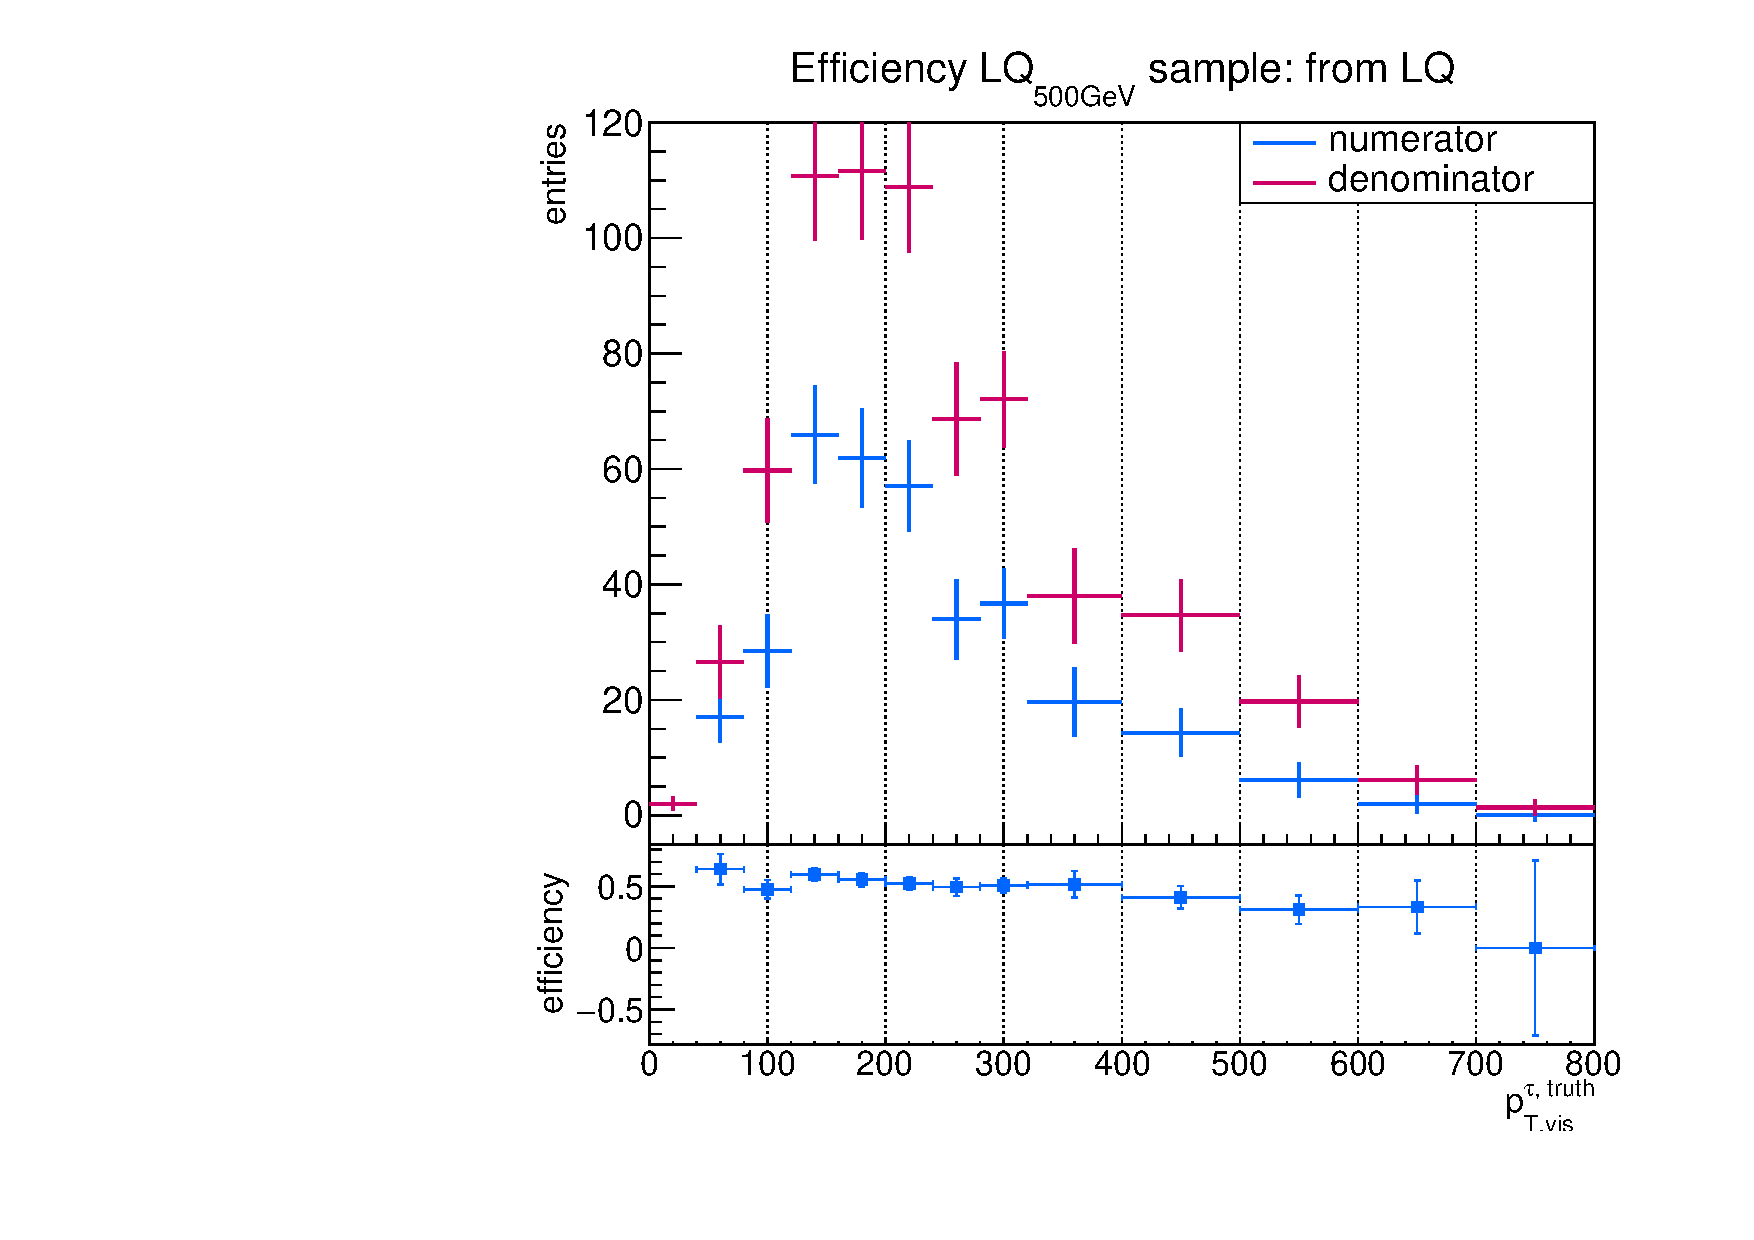
\includegraphics[width=\textwidth]{figures/plots/LQ75/Divided_LQ.pdf}
                \subcaption{Efficiency of taus originating LQs of $\SI{51.3\pm 1.2}{\percent}$ for the low mass LQ events.}
                \label{DividedfromLQ:signal:allLQ75}
                \end{subfigure}
                %
                \begin{subfigure}[t]{0.49\textwidth}
                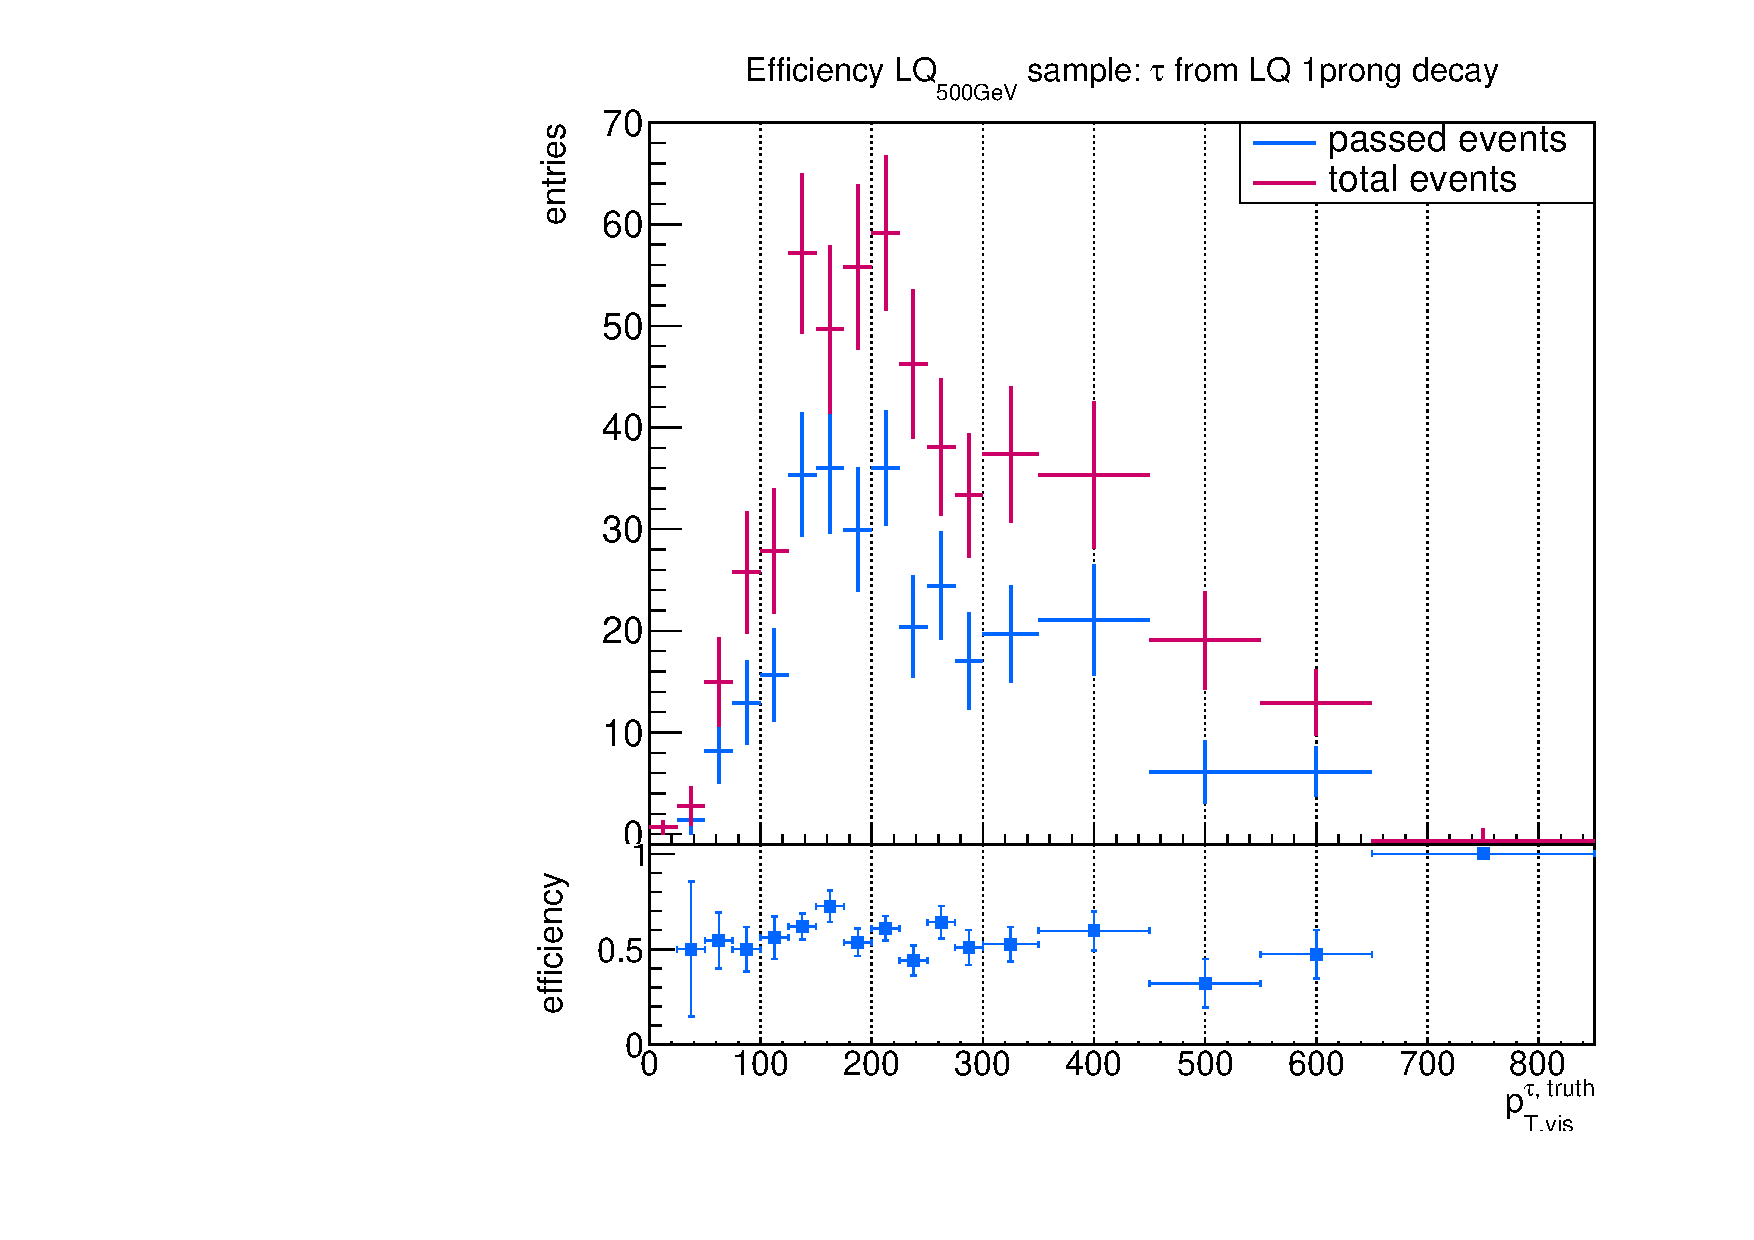
\includegraphics[width=\textwidth]{figures/plots/LQ75/Divided_fromLQ1prong.pdf}
                \subcaption{Efficiency of taus originating LQs and decaying in the 1-prong mode. The efficiency is $\SI{55.5\pm 1.4}{\percent}$ for the low mass LQ events.}
                \label{DividedfromLQ:signal:1prongLQ75}
                \end{subfigure}
                %
                \begin{subfigure}[t]{0.49\textwidth}
                \includegraphics[width=\textwidth]{figures/plots/LQ75/Divided_fromLQ3prong.pdf}
                \subcaption{Efficiency of taus originating LQs and decaying in the 3-prong mode. The efficiency is $\SI{38.2\pm 2.4}{\percent}$ for the low mass LQ events.}
                \label{DividedfromLQ:signal:3prong}
                \end{subfigure}
\caption[Efficiency of taus originating LQs for the low mass LQ signal events.]{Efficiency of taus originating LQs for the low mass LQ signal events. The efficiency is defined as the number of taus matched to a hadronic truth tau over the number of truth taus passing the basic selection.}
\label{DividedFromLQ:signal:LQ75}
\end{figure}
%
%
\begin{figure}
  \centering
                \begin{subfigure}[t]{0.49\textwidth}
                \includegraphics[width=\textwidth]{figures/plots/LQ76/Divided_LQ.pdf}
                \subcaption{Efficiency of taus originating LQs of $\SI{50.7\pm 1.5}{\percent}$ for the high mass LQ events.}
                \label{DividedfromLQ:signal:allLQ76}
                \end{subfigure}
                %
                \begin{subfigure}[t]{0.49\textwidth}
                \includegraphics[width=\textwidth]{figures/plots/LQ76/Divided_fromLQ1prong.pdf}
                \subcaption{Efficiency of taus originating LQs and decaying in the 1-prong mode. The efficiency is $\SI{55.0\pm 1.7}{\percent}$ for the high mass LQ events.}
                \label{DividedfromLQ:signal:1prongLQ76}
                \end{subfigure}
                %
                \begin{subfigure}[t]{0.49\textwidth}
                \includegraphics[width=\textwidth]{figures/plots/LQ76/Divided_fromLQ3prong.pdf}
                \subcaption{Efficiency of taus originating LQs and decaying in the 3-prong mode. The efficiency is $\SI{36.3\pm 3.0}{\percent}$ for the high mass LQ events.}
                \label{DividedfromLQ:signal:3prongLQ76}
                \end{subfigure}            
\caption[Efficiency of taus originating LQs for the high mass LQ signal events.]{Efficiency of taus originating LQs for the high mass LQ signal events. The efficiency is defined as the number of taus matched to a hadronic truth tau over the number of truth taus passing the basic selection.}
\label{DividedFromLQ:signal:LQ76}
\end{figure}
%
For the high mass point leptoquarks the efficiency dependence on the taus' transverse momentum is constantly over the whole momentum range (see fig. \ref{DividedFromLQ:signal:LQ76}). Like for the low mass point, the 1-prong case reveals no considerable dependence on the taus' $p_T$. More fluctuations in efficiency can be observed in case of 3-prong (see fig. \ref{DividedfromLQ:signal:3prongLQ76}). The slight efficiency decrease for the low mass point sample could be an effect due to the higher mass point of the second LQ sample and the resulting more expanded $p_T$ spectrum, because it shows not such effects.  
%HT,ST Gedöns prompt | LQ
The dependence of the efficiency on kinematic variables like $H_T$, $H_{T,\text{had}}$, $S_T$, $S_{T,\text{lep}}$ defined in eq. (\ref{STlepgedöns})-(\ref{HTgedöns}) and the number of jets is also available for the leptoquark related events. \newline
%HT und HThad
%Figure \ref{Dividedprompt:signal:HTgedöns} shows the efficiency depending on the variable $H_T$ and $H_{T,\text{had}}$ for the sub-selections, where taus originate from weak gauge bosons.
The dependence between $H_{T}$ ($H_{T,\text{had}}$) and the efficiency in case of the sub-category, where tau leptons originate from LQs, are shown in figure \ref{DividedFromLQ:signal:HTgedöns}. The $H_T$ ($H_{T,\text{had}}$) spectrum covers a larger range for the $\SI{1}{\tera\electronvolt}$ leptoquarks sample due to its higher mass. The $H_T$ distribution extends up to $\SI{3}{\tera\electronvolt}$ (see fig. \ref{DividedFromLQ:signal:HTLQ76}) compared to figure \ref{DividedFromLQ:signal:HTLQ75}, which extends only to $\SI{2.5}{\tera\electronvolt}$. The $H_{T,\text{had}}$ distribution extends up to $\SI{2.5}{\tera\electronvolt}$ (see fig. \ref{DividedFromLQ:signal:HThadLQ76}) compared to figure \ref{DividedFromLQ:signal:HThadLQ75}, which extends to $\SI{1.2}{\tera\electronvolt}$. The efficiency trend over the whole spectrum is constant besides some fluctuations.\newline
%
\begin{figure}
  \centering
                \begin{subfigure}[t]{0.49\textwidth}
                \includegraphics[width=\textwidth]{figures/plots/LQ75/Divided_fromLQHT.pdf}
                \subcaption{Efficiency of taus originating from leptoquarks of depending on $H_{T}$ low mass LQ sample.}
                \label{DividedFromLQ:signal:HTLQ75}
                \end{subfigure}
                %
                \begin{subfigure}[t]{0.49\textwidth}
                \includegraphics[width=\textwidth]{figures/plots/LQ75/Divided_fromLQHThad.pdf}
                \subcaption{Efficiency of taus originating from leptoquarks of depending on $H_{T,\text{had}}$ low mass LQ sample.}
                \label{DividedFromLQ:signal:HThadLQ75}
                \end{subfigure}
                %
                \begin{subfigure}[t]{0.49\textwidth}
                \includegraphics[width=\textwidth]{figures/plots/LQ76/Divided_fromLQHT.pdf}
                \subcaption{Efficiency of taus originating from leptoquarks of depending on $H_{T}$ high mass LQ sample.}
                \label{DividedFromLQ:signal:HTLQ76}
                \end{subfigure}
                %
                \begin{subfigure}[t]{0.49\textwidth}
                \includegraphics[width=\textwidth]{figures/plots/LQ76/Divided_fromLQHThad.pdf}
                \subcaption{Efficiency of taus originating from leptoquarks of depending on $H_{T,\text{had}}$ high mass LQ sample.}
                \label{DividedFromLQ:signal:HThadLQ76}
                \end{subfigure}
\caption[Efficiency of taus originating from leptoquarks for the LQ signal events.]{Efficiency of taus originating from leptoquarks depending on $H_{T}$ (a), (c) and $H_{T,\text{had}}$ (b), (d) for the LQ signal events.}
\label{DividedFromLQ:signal:HTgedöns}
\end{figure}
%
%ST und STlep
Taking into account not only jets, electrons and muons, but also taus and missing energy for example one can study the correlation between the efficiency and $S_T$ ($S_{T,\text{lep}}$). This is done in figure \ref{DividedFromLQ:signal:STgedöns} for taus originating from Higgs bosons. The efficiency depends only slightly on the variable $S_T$ (see fig. \ref{DividedFromLQ:signal:STLQ75}) or $S_{T,\text{lep}}$ (see fig. \ref{DividedFromLQ:signal:STlepLQ75}) over the whole spectrum, whereas in case of the more massive LQ sample the efficiency increases towards the high momenta end of the spectrum. This involves the range of $\SI{2600}{\giga\electronvolt}$ onwards for $S_T$ and $\SI{2000}{\giga\electronvolt}$ onwards for $S_{T,\text{lep}}$. This difference can exist because of the different mass points of the leptoquarks. The spectrum of the $\SI{1}{\tera\electronvolt}$ naturally extends to a higher momenta values.\newline
%
\begin{figure}
  \centering
                \begin{subfigure}[t]{0.49\textwidth}
                \includegraphics[width=\textwidth]{figures/plots/LQ75/Divided_fromLQST.pdf}
                \subcaption{Efficiency of taus originating from leptoquarks of depending on $S_{T}$ low mass LQ sample.}
                \label{DividedFromLQ:signal:STLQ75}
                \end{subfigure}
                %
                \begin{subfigure}[t]{0.49\textwidth}
                \includegraphics[width=\textwidth]{figures/plots/LQ75/Divided_fromLQSTlep.pdf}
                \subcaption{Efficiency of taus originating from leptoquarks of depending on $S_{T,\text{lep}}$ low mass LQ sample.}
                \label{DividedFromLQ:signal:STlepLQ75}
                \end{subfigure}
                %
                \begin{subfigure}[t]{0.49\textwidth}
                \includegraphics[width=\textwidth]{figures/plots/LQ76/Divided_fromLQST.pdf}
                \subcaption{Efficiency of taus originating from leptoquarks of depending on $S_{T}$ high mass LQ sample.}
                \label{DividedFromLQ:signal:STLQ76}
                \end{subfigure}
                %
                \begin{subfigure}[t]{0.49\textwidth}
                \includegraphics[width=\textwidth]{figures/plots/LQ76/Divided_fromLQSTlep.pdf}
                \subcaption{Efficiency of taus originating from leptoquarks of depending on $S_{T,\text{lep}}$ high mass LQ sample.}
                \label{DividedFromLQ:signal:STlepLQ76}
                \end{subfigure}
\caption[Efficiency of taus originating from leptoquarks for the LQ signal events.]{Efficiency of taus originating from leptoquarks depending on $S_{T}$ (a), (c) and $S_{T,\text{lep}}$ (b), (d) for the LQ signal events.}
\label{DividedFromLQ:signal:STgedöns}
\end{figure}
%
%njets
The jet multiplicity depicted against the efficiency can be found in figure \ref{Divided:fromLQ:njets} and shows an interesting feature in both LQ samples. No tau entries for two jets survived the condition that taus are directly from LQ and matched to a truth tau. The low efficiency for two jets in case of the $t\bar{t}H$ sample (see fig. \ref{Divided:fromH:njets}) may indicate that the already tight conditions for two jets evoked in case of taus originating from LQ that no event survives. 
%
\begin{figure}
  \centering
                \begin{subfigure}[t]{0.49\textwidth}
                \includegraphics[width=\textwidth]{figures/plots/LQ75/Divided_fromLQnjets.pdf}
                \subcaption{Efficiency of taus originating from LQs depending on the number of jets for the LQ sample with low mass point.}
                \label{DividedFromLQ:signal:njetsLQ75}
                \end{subfigure}
                %
                \begin{subfigure}[t]{0.49\textwidth}
                \includegraphics[width=\textwidth]{figures/plots/LQ76/Divided_fromLQnjets.pdf}
                \subcaption{Efficiency of taus originating from LQs depending on the number of jets for the LQ sample with high mass point.}
                \label{DividedFromLQ:signal:njetsLQ76}
                \end{subfigure}
\caption[Efficiency of taus originating from LQs depending on the number of jets.]{Efficiency of taus originating from LQs depending on the number of jets.}
\label{Divided:fromLQ:njets}
\end{figure}
%
%dR min max Gedöns LQ
The following describes the geometric separation between taus and leptons, taus and jets as well as taus and b-jets for the LQ signal samples.\newline
%dR taulepton
The minimum separation between taus and light leptons (electrons and muons) is shown in figure \ref{dRFromLQ:signal:taulepton} for both signal samples. It is the efficiency for taus originating from $H^0$ bosons. The minimum separation is not only concentrated on a small $\Delta R$ range, but extends over the whole separation spectrum. A maximum number of taus with minimal separation can be found at $\Delta R=1.6$ in case of the low mass point sample. Below $\Delta R<0.4$ no taus can be found, which is explained by the overlap removal (cf. section \ref{overlapremoval}). The maximum separation for the $\SI{500}{\giga\electronvolt}$ sample (see fig. \ref{dRFromLQ:signal:taulepton:maxLQ75}) indicates most tau events at $\Delta R=3.0$. Below $\Delta R<0.8$ no entry can be found. An interesting feature is that for the maximum separation two efficiency peaks are present at a separation of $1.0$ and $1.6$. For the $\SI{1}{\tera\electronvolt}$ signal sample the minimum separation (see fig. \ref{dRFromLQ:signal:taulepton:minLQ76}) does not undercut the value of $0.4$ which can be explained again by the overlap removal. Comparing figure \ref{dRFromLQ:signal:taulepton:minLQ75} and \ref{dRFromLQ:signal:taulepton:minLQ76} shows that in case of the high mass point LQ sample no maximum number of taus can be found around $\Delta R=1.6$. In this case it is more a plateau. Again, two efficiency peaks show up at a separation of $1.0$ and $2.0$. The maximum separation (see fig. \ref{dRFromLQ:signal:taulepton:maxLQ76}) indicates slightly higher efficiency at the end of the separation distribution.\newline     
%
\begin{figure}
  \centering
                \begin{subfigure}[t]{0.49\textwidth}
                \includegraphics[width=\textwidth]{figures/plots/LQ75/Divided_fromLQ_mindR_taulepton.pdf}
                \subcaption{Minimum separation between taus originating from LQs events and leptons for the low mass point LQ sample.}
                \label{dRFromLQ:signal:taulepton:minLQ75}
                \end{subfigure}
                %
                \begin{subfigure}[t]{0.49\textwidth}
                \includegraphics[width=\textwidth]{figures/plots/LQ75/Divided_maxdR_fromLQ_taulepton.pdf}
                \subcaption{Maximum separation between taus originating from LQs events and leptons for the low mass point LQ sample.}
                \label{dRFromLQ:signal:taulepton:maxLQ75}
                \end{subfigure}
                 %
                \begin{subfigure}[t]{0.49\textwidth}
                \includegraphics[width=\textwidth]{figures/plots/LQ76/Divided_fromLQ_mindR_taulepton.pdf}
                \subcaption{Minimum separation between taus originating from LQs events and leptons for the high mass point LQ sample.}
                \label{dRFromLQ:signal:taulepton:minLQ76}
                \end{subfigure}
                 %
                \begin{subfigure}[t]{0.49\textwidth}
                \includegraphics[width=\textwidth]{figures/plots/LQ76/Divided_maxdR_fromLQ_taulepton.pdf}
                \subcaption{Maximum separation between taus originating from LQs events and leptons for the high mass point LQ sample.}
                \label{dRFromLQ:signal:taulepton:maxLQ76}
                \end{subfigure}
\caption[Efficiency of separation between taus originating from LQs and leptons.]{Efficiency of minimum and maximum separation between taus originating from LQs and leptons (electrons and muons).}
\label{dRFromLQ:signal:taulepton}
\end{figure}
%
Correspondingly to the background samples the minimum and maximum separation between taus and jets is shown in figure \ref{dRFromLQ:signal:taujet} for taus originating directly from LQs. Similar to the separation in the $t\bar{t}H$ sample (cf. figure \ref{dR:fromH:taujets}) the minimum separation has only high efficiency values at $\Delta R<0.5$ and no entries otherwise in the spectrum. This can be explained by the jet fake rates, which are expected in that separation region. The maximum separation for both signal samples resembles in prinicple that from the $t\bar{t}H$ sample with the most taus at a separation of $3.0$. No number of taus are found below $\Delta R=1.2$ and $\Delta R=1.4$ for the low and high mass point signal sample respectively. \newline
%\ref{dRprompt:signal:taujet} $W^\pm$ and $Z^0$ and in figure \ref{dRFromLQ:signal:taujet} for taus originating directly from LQs.\newline
%
\begin{figure}
  \centering
                \begin{subfigure}[t]{0.49\textwidth}
                \includegraphics[width=\textwidth]{figures/plots/LQ75/Divided_fromLQ_mindR_taujet.pdf}
                \subcaption{Minimum separation between taus originating from LQs events and jets for the low mass point LQ sample.}
                \label{dRFromLQ:signal:taujet:minLQ75}
                \end{subfigure}
                %
                \begin{subfigure}[t]{0.49\textwidth}
                \includegraphics[width=\textwidth]{figures/plots/LQ75/Divided_maxdR_fromLQ_taujet.pdf}
                \subcaption{Maximum separation between taus originating from LQs events and jets for the low mass point LQ sample.}
                \label{dRFromLQ:signal:taujet:maxLQ75}
                \end{subfigure}
                 %
                \begin{subfigure}[t]{0.49\textwidth}
                \includegraphics[width=\textwidth]{figures/plots/LQ76/Divided_fromLQ_mindR_taujet.pdf}
                \subcaption{Minimum separation between taus originating from LQs events and jets for the high mass point LQ sample.}
                \label{dRFromLQ:signal:taujet:minLQ76}
                \end{subfigure}
                 %
                \begin{subfigure}[t]{0.49\textwidth}
                \includegraphics[width=\textwidth]{figures/plots/LQ76/Divided_maxdR_fromLQ_taujet.pdf}
                \subcaption{Maximum separation between taus originating from LQs events and jets for the high mass point LQ sample.}
                \label{dRFromLQ:signal:taujet:maxLQ76}
                \end{subfigure}
\caption[Efficiency of separation between taus originating from LQs and jets.]{Efficiency of minimum and maximum separation between taus originating from LQs and jets.}
\label{dRFromLQ:signal:taujet}
\end{figure}
%
%The special case of the minimum and maximum separation between taus and b-flavor jets is shown in figure \ref{dRprompt:signal:taubjet} for the sub-category taus originating from $W^\pm$ and $Z^0$ bosons.
The special case of the minimum and maximum separation between taus and b-flavor jets is shown in figure \ref{dRFromLQ:signal:taubjet} for the sub-category taus originating from LQs. The separation between taus and b-jets in the $\SI{500}{\giga\electronvolt}$ sample show a broad spectrum over the whole separation range. The minimum separation (see fig. \ref{dRFromLQ:signal:taubjet:minLQ75}) and maximum separation (see fig. \ref{dRFromLQ:signal:taubjet:maxLQ75}) show two efficiency peaks within the range of $1.0<\Delta R<2.0$ and $1.0<\Delta R<2.2$ respectively. Small contributions are found for the minimum separation at $<0.4$ (see fig. \ref{dRFromLQ:signal:taubjet:minLQ76}). The $\SI{1}{\tera\electronvolt}$ sample also shows low efficiency in the range of $<0.4$ for the minumum separation. Again peaks of efficiency show up here in the range of $1.0$ and $1.4$ for the minimum and maximum separation (see fig. \ref{dRFromLQ:signal:taubjet:maxLQ76}) respectively.
%The separation between taus and b-jets in case of the sub-selection, where taus originate from LQs are shown in figure \ref{dRFromLQ:signal:taubjet}.
%
\begin{figure}
  \centering
                \begin{subfigure}[t]{0.49\textwidth}
                \includegraphics[width=\textwidth]{figures/plots/LQ75/Divided_mindR_fromLQ_taubjet.pdf}
                \subcaption{Minimum separation between taus originating from LQs events and b-jets for the low mass point LQ sample.}
                \label{dRFromLQ:signal:taubjet:minLQ75}
                \end{subfigure}
                %
                \begin{subfigure}[t]{0.49\textwidth}
                \includegraphics[width=\textwidth]{figures/plots/LQ75/Divided_maxdR_fromLQ_taubjet.pdf}
                \subcaption{Maximum separation between taus originating from LQs events and b-jets for the low mass point LQ sample.}
                \label{dRFromLQ:signal:taubjet:maxLQ75}
                \end{subfigure}
                 %
                \begin{subfigure}[t]{0.49\textwidth}
                \includegraphics[width=\textwidth]{figures/plots/LQ76/Divided_mindR_fromLQ_taubjet.pdf}
                \subcaption{Minimum separation between taus originating from LQs events and b-jets for the high mass point LQ sample.}
                \label{dRFromLQ:signal:taubjet:minLQ76}
                \end{subfigure}
                 %
                \begin{subfigure}[t]{0.49\textwidth}
                \includegraphics[width=\textwidth]{figures/plots/LQ76/Divided_maxdR_fromLQ_taubjet.pdf}
                \subcaption{Maximum separation between taus originating from LQs events and b-jets for the high mass point LQ sample.}
                \label{dRFromLQ:signal:taubjet:maxLQ76}
                \end{subfigure}
\caption[Efficiency of separation between taus originating from LQs and b-jets.]{Efficiency of minimum and maximum separation between taus originating from LQs and b-jets.}
\label{dRFromLQ:signal:taubjet}
\end{figure}
%
\section{Kinematics}\label{Kinematics}
%%%%%%%%%%%%%%%%%%%%%%%%%%%%%%%%%%%%%%%%%%%%%%%%%%%%%%%%%%%%%%%%%%%%%%%%%%%%%%%%%%%%%%%%%%%%%%%%%%%%%%%%%%%%%
%%%%%%%%%%%%%%%%%%%%%%%%%%%%%%%%%%%%%%%%%%%%%%%%%%%%%%%%%%%%%%%%%%%%%%%%%%%%%%%%%%%%%%%%%%%%%%%%%%%%%%%%%%%%%
%%%%%%%%%%%%%%%%%%%%%%%%%%%%%%%%%%%%%%%%%%%%%%%%%%%%%%%%%%%%%%%%%%%%%%%%%%%%%%%%%%%%%%%%%%%%%%%%%%%%%%%%%%%%%
%%%%%%%%%%%%%%%%%%%%%%%%%%%%%%%%%%%%%%%%%%%%%%%%%%%%%%%%%%%%%%%%%%%%%%%%%%%%%%%%%%%%%%%%%%%%%%%%%%%%%%%%%%%%%
%%%%%%%%%%%%%%%%%%%%%%%%%%%%%%%%%%%%%%%%%%%%%%%%%%%%%%%%%%%%%%%%%%%%%%%%%%%%%%%%%%%%%%%%%%%%%%%%%%%%%%%%%%%%%
%%%%%%%%%%%%%%%%%%%%%%%%%%%%%%%%%%%%%%%%%%%%%%%%%%%%%%%%%%%%%%%%%%%%%%%%%%%%%%%%%%%%%%%%%%%%%%%%%%%%%%%%%%%%%
The signal and background efficiencies in section \ref{signalANDbgEff} help to understand especially the role of the tau lepton for the relevant $t\tau^{-}+\bar{t}\tau^{+}$ channel. The next step into the direction of signal studies is to compare the event yield for signal and background samples in the different channels of the event selection (cf. section \ref{eventselection}). This is done by studying kinematic variables for the tau lepton like the transverse momentum, angular distribution, the variables defined in eq. (\ref{STlepgedöns})-(\ref{HTgedöns}) (cf. section \ref{bgeff}) and the separation between taus and objects like electrons, jets and b-jets. The comparison is done with the background and signal MC samples together with data of the data-taking years 2015 until 2018. This reveals, if the signature of the chosen event selection can be extracted and detected within the known standard model processes. The data in this context gives the possibility of reference how well data is resembled by the MC simulation, although this work is not a full LQ search. No systematic variations are applied on the Monte Carlo simulations, which would be the normal procedure for a full search. For data the luminosity of \SI{140}{\per\femto\barn} (cf. table \ref{datalumi}) is available.\par
%tau pT
The transverse momentum distribution of all tau leptons is shown in figure \ref{taupt} for different event selections.
%
\begin{figure}
  \centering
                \begin{subfigure}[t]{0.49\textwidth}
                \includegraphics[width=\textwidth]{figures/plots/kinLQ75/tau_pT_2j2b_1tau.pdf}
                \subcaption{$p_T$ distribution of the tau leptons, when selecting at least two b-jets and at least one additional tau.}
                \label{taupt:2b1tau}
                \end{subfigure}
                %
                \begin{subfigure}[t]{0.49\textwidth}
                \includegraphics[width=\textwidth]{figures/plots/kinLQ75/tau_pT_2j2b_2tau.pdf}
                \subcaption{$p_T$ distribution of the tau leptons, when selecting at least two b-jets and at least two additional tau.}
                \label{taupt:2b2tau}
                \end{subfigure}
                 %
                \begin{subfigure}[t]{0.49\textwidth}
                \includegraphics[width=\textwidth]{figures/plots/kinLQ75/tau_pT_2j1b_1tau.pdf}
                \subcaption{$p_T$ distribution of the tau leptons, when selecting at least one b-jets and at least one additional tau.}
                \label{taupt:1b1tau}
                \end{subfigure}
                 %
                \begin{subfigure}[t]{0.49\textwidth}
                \includegraphics[width=\textwidth]{figures/plots/kinLQ75/tau_pT_2j1b_2tau.pdf}
                \subcaption{$p_T$ distribution of the tau leptons, when selecting at least one b-jets and at least two additional tau.}
                \label{taupt:1b2tau}
                \end{subfigure}
\caption[Transverse momentum distribution of all tau leptons for different event selections.]{Transverse momentum distribution of all tau leptons for different event selections.}
\label{taupt}
\end{figure}
%
The selection of at least two b-jets and at least one tau shows (see figure \ref{taupt:2b1tau}) that up to transverse momenta of $\SI{80}{\giga\electronvolt}$ the LQ signal is hidden from top-quark pair and Higgs contributions. But from that threshold on the momentum distribution of the low mass signal sample exceeds the background. For the high mass point sample this happens at $\SI{360}{\giga\electronvolt}$. The MC background samples agree well with data from $\SI{50}{\giga\electronvolt}$ onward, besides one outlier. Before that value data exceeds the background taken into account. The discrepancy can be explained such that more contributions should be taken into account like vector bosons and additional jets, di-boson events or single-top contributions. Tightening the selection to at least two taus (see figure \ref{taupt:2b2tau}) will reveal even more signal compared to relatively small background. The event yield for data shows that only few events in this selection is expected. The disadvantage in this selection is the few events in general, which results in low statistics. The looser selection of taking only at least one b-jet and at least one tau (see figure \ref{taupt:1b1tau}) shifts the threshold for the signal up to $\SI{100}{\giga\electronvolt}$ and $\SI{350}{\giga\electronvolt}$ for the low and high mass point LQ sample respectively, but allows at the same time higher statistics. This effect is clearly visible in the selection of at least one b-jet and at least two tau leptons shown in figure \ref{taupt:1b2tau}. The discrepancy between data and MC in the lower $p_T$ range also exists here, as it depends not directly on the chosen selection. The transverse momentum of taus in data does not exceed \SI{350}{\giga\electronvolt} and $\SI{150}{\giga\electronvolt}$ for the selection with at least one tau and at least two taus respectively. This would be interesting threshold for $p_T$ cuts to optimize the signal (see also section \ref{significance}).\par
%tauphi
The distribution of the azimuthal angle of the tau leptons for different event selection is shown in figure \ref{tauphi}. It gives the same picture as for the transverse momentum distribution including the lack of MC events. For the selection of at least two b-jets and at least one tau the signal samples are hidden by the background over the whole $\phi$ range (see figure \ref{tauphi:2b1tau} and \ref{tauphi:1b1tau}). Only the at least two tau selection reveals the LQ signal. Better statistics can be achieved by using the selection with at least one b-jet and at least two taus (see figure \ref{tauphi:1b2tau}).\par
%
\begin{figure}
  \centering
                \begin{subfigure}[t]{0.49\textwidth}
                \includegraphics[width=\textwidth]{figures/plots/kinLQ75/tau_phi_2j2b_1tau.pdf}
                \subcaption{$\phi$ distribution of the tau leptons, when selecting at least two b-jets and at least one additional tau.}
                \label{tauphi:2b1tau}
                \end{subfigure}
                %
                \begin{subfigure}[t]{0.49\textwidth}
                \includegraphics[width=\textwidth]{figures/plots/kinLQ75/tau_phi_2j2b_2tau.pdf}
                \subcaption{$\phi$ distribution of the tau leptons, when selecting at least two b-jets and at least two additional tau.}
                \label{tauphi:2b2tau}
                \end{subfigure}
                 %
                \begin{subfigure}[t]{0.49\textwidth}
                \includegraphics[width=\textwidth]{figures/plots/kinLQ75/tau_phi_2j1b_1tau.pdf}
                \subcaption{$\phi$ distribution of the tau leptons, when selecting at least one b-jets and at least one additional tau.}
                \label{tauphi:1b1tau}
                \end{subfigure}
                 %
                \begin{subfigure}[t]{0.49\textwidth}
                \includegraphics[width=\textwidth]{figures/plots/kinLQ75/tau_phi_2j1b_2tau.pdf}
                \subcaption{$\phi$ distribution of the tau leptons, when selecting at least one b-jets and at least two additional tau.}
                \label{tauphi:1b2tau}
                \end{subfigure}
\caption[Azimuthal angle distribution of all tau leptons for different event selections.]{Azimuthal angle distribution of all tau leptons for different event selections.}
\label{tauphi}
\end{figure}
%
%tau eta
The pseudorapidity distribution shows the same trend as the $p_T$ and $\phi$ distribution described above and is shown in figure \ref{taueta}. Although the $\eta$ distribution of the LQ signal has more events concentrated in the region of roughly $|\eta|<1.5$ compared to the standard model prediction and data, this difference in shape cannot be used as discriminating variable. The background hides too much in with this selection. Even the high mass point LQ sample can not be extracted in the selection of at least two taus. In general the high $p_T$ range and the selection of two taus is more dominated from Higgs background processes, whereas the top-quark pair background processes cover the lower transverse momentum range and selection with less than two taus. This is due to real tau production in the $t\bar{t}H$ sample. \par
%
\begin{figure}
  \centering
                \begin{subfigure}[t]{0.49\textwidth}
                \includegraphics[width=\textwidth]{figures/plots/kinLQ75/tau_eta_2j2b_1tau.pdf}
                \subcaption{$\eta$ distribution of the tau leptons, when selecting at least two b-jets and at least one additional tau.}
                \label{taueta:2b1tau}
                \end{subfigure}
                %
                \begin{subfigure}[t]{0.49\textwidth}
                \includegraphics[width=\textwidth]{figures/plots/kinLQ75/tau_eta_2j2b_2tau.pdf}
                \subcaption{$\eta$ distribution of the tau leptons, when selecting at least two b-jets and at least two additional tau.}
                \label{taueta:2b2tau}
                \end{subfigure}
                 %
                \begin{subfigure}[t]{0.49\textwidth}
                \includegraphics[width=\textwidth]{figures/plots/kinLQ75/tau_eta_2j1b_1tau.pdf}
                \subcaption{$\eta$ distribution of the tau leptons, when selecting at least one b-jets and at least one additional tau.}
                \label{taueta:1b1tau}
                \end{subfigure}
                 %
                \begin{subfigure}[t]{0.49\textwidth}
                \includegraphics[width=\textwidth]{figures/plots/kinLQ75/tau_eta_2j1b_2tau.pdf}
                \subcaption{$\eta$ distribution of the tau leptons, when selecting at least one b-jets and at least two additional tau.}
                \label{taueta:1b2tau}
                \end{subfigure}
\caption[Pseudorapidity distribution of all taus lepton for different event selections.]{Pseudorapidity distribution of all tau leptons for different event selections.}
\label{taueta}
\end{figure}
%
%MET
Following the definition of eq. \ref{STgedöns} (cf. section \ref{bgeff}) the distribution of the missing energy for different selections is shown in figure \ref{MET}. The missing energy is not a optimal discriminant variable, because the signal is not well separated over the whole $\cancel{E}_T$ range in the selection of at least one b-jet and at least one tau (see \ref{MET:1b1tau}). The signal is in fact better separated in the selection of at least two b-jets and at least one tau as depicted in figure \ref{MET:2b1tau}. The at least two tau condition improves the separation (see figure \ref{MET:2b2tau} and \ref{MET:1b2tau}) between signal and background. Although the studied $t\tau^{-}+\bar{t}\tau^{+}$ channel has sources of neutrinos responsible for missing transverse energy through the decay of tau leptons or leptonic $W^\pm$ decays, this is not enough to discriminate it from background neutrino contributions. Again, at least two taus selected induces a more $t\bar{t}H$ dominated background. \par   
%
\begin{figure}
  \centering
                \begin{subfigure}[t]{0.49\textwidth}
                \includegraphics[width=\textwidth]{figures/plots/kinLQ75/MET_2j2b_1tau.pdf}
                \subcaption{$\cancel{E}_T$ distribution, when selecting at least two b-jets and at least one additional tau.}
                \label{MET:2b1tau}
                \end{subfigure}
                %
                \begin{subfigure}[t]{0.49\textwidth}
                \includegraphics[width=\textwidth]{figures/plots/kinLQ75/MET_2j2b_2tau.pdf}
                \subcaption{$\cancel{E}_T$ distribution, when selecting at least two b-jets and at least two additional tau.}
                \label{MET:2b2tau}
                \end{subfigure}
                 %
                \begin{subfigure}[t]{0.49\textwidth}
                \includegraphics[width=\textwidth]{figures/plots/kinLQ75/MET_2j1b_1tau.pdf}
                \subcaption{$\cancel{E}_T$ distribution, when selecting at least one b-jets and at least one additional tau.}
                \label{MET:1b1tau}
                \end{subfigure}
                 %
                \begin{subfigure}[t]{0.49\textwidth}
                \includegraphics[width=\textwidth]{figures/plots/kinLQ75/MET_2j1b_2tau.pdf}
                \subcaption{$\cancel{E}_T$ distribution, when selecting at least one b-jets and at least two additional tau.}
                \label{MET:1b2tau}
                \end{subfigure}
\caption[Missing energy distribution for different event selections.]{Missing energy distribution for different event selections.}
\label{MET}
\end{figure}
%
%HT
The distribution of $H_T$ is shown in figure \ref{HT}. Because this distribution is the sum of the transverse momenta of electrons, muons and jets this is good discriminating variable for particles with high masses like the leptoquarks. High masses like the $\SI{0.5}{\tera\electronvolt}$ or even $\SI{1}{\tera\electronvolt}$ produce a broader $H_T$ spectrum extending to higher transverse momenta, which then in turn can be distinguished from standard model events. Figure \ref{HT:2b1tau} shows that the background decreases from $\SI{600}{\giga\electronvolt}$ on and reveals at least the $\SI{500}{\giga\electronvolt}$ mass LQ signal. The selection of at least one tau is not sufficient for the high LQ mass point. The best extraction results are gained from selecting at least two taus and is shown in figure \ref{HT:2b2tau} and \ref{HT:1b2tau}. These two selections again show that the $t\bar{t}H$ events are more dominant for the two tau selection due to its abundant tau events. Data has higher event numbers for the selection with at least one tau, which can be explained by the lack of additional contributions. Nevertheless for two tau selection it is a good approximation. The statistics is higher for the selection of at least two b-jets.\par    
%
\begin{figure}
  \centering
                \begin{subfigure}[t]{0.49\textwidth}
                \includegraphics[width=\textwidth]{figures/plots/kinLQ75/HT_2j2b_1tau.pdf}
                \subcaption{$H_T$ distribution of the tau leptons, when selecting at least two b-jets and at least one additional tau.}
                \label{HT:2b1tau}
                \end{subfigure}
                %
                \begin{subfigure}[t]{0.49\textwidth}
                \includegraphics[width=\textwidth]{figures/plots/kinLQ75/HT_2j2b_2tau.pdf}
                \subcaption{$H_T$ distribution of the tau leptons, when selecting at least two b-jets and at least two additional tau.}
                \label{HT:2b2tau}
                \end{subfigure}
                 %
                \begin{subfigure}[t]{0.49\textwidth}
                \includegraphics[width=\textwidth]{figures/plots/kinLQ75/HT_2j1b_1tau.pdf}
                \subcaption{$H_T$ distribution of the tau leptons, when selecting at least one b-jets and at least one additional tau.}
                \label{HT:1b1tau}
                \end{subfigure}
                 %
                \begin{subfigure}[t]{0.49\textwidth}
                \includegraphics[width=\textwidth]{figures/plots/kinLQ75/HT_2j1b_2tau.pdf}
                \subcaption{$H_T$ distribution of the tau leptons, when selecting at least one b-jets and at least two additional tau.}
                \label{HT:1b2tau}
                \end{subfigure}
\caption[$H_T$ distribution of the tau lepton for different event selections.]{$H_T$ distribution of the tau lepton for different event selections.}
\label{HT}
\end{figure}
%
%HThad
The variable $H_{T,\text{had}}$ in principle shows the same trend as the $H_T$ distribution for a discriminating variable. Nevertheless the effect of extracting the signal is not as good as for $H_T$. The reason is that less objects are included in the variable. $H_{T,\text{had}}$ only contains the sum of the jets' momenta. The plots are shown in figure \ref{HThad}. As a conclusion drawn from the comparison of $H_T$ and $H_{T,\text{had}}$ distribution is that the discrimination is better for variables containing more objects. \par
%
\begin{figure}
  \centering
                \begin{subfigure}[t]{0.49\textwidth}
                \includegraphics[width=\textwidth]{figures/plots/kinLQ75/HThad_2j2b_1tau.pdf}
                \subcaption{$H_{T,\text{had}}$ distribution of the tau leptons, when selecting at least two b-jets and at least one additional tau.}
                \label{HThad:2b1tau}
                \end{subfigure}
                %
                \begin{subfigure}[t]{0.49\textwidth}
                \includegraphics[width=\textwidth]{figures/plots/kinLQ75/HThad_2j2b_2tau.pdf}
                \subcaption{$H_{T,\text{had}}$ distribution of the tau leptons, when selecting at least two b-jets and at least two additional tau.}
                \label{HThad:2b2tau}
                \end{subfigure}
                 %
                \begin{subfigure}[t]{0.49\textwidth}
                \includegraphics[width=\textwidth]{figures/plots/kinLQ75/HThad_2j1b_1tau.pdf}
                \subcaption{$H_{T,\text{had}}$ distribution of the tau leptons, when selecting at least one b-jets and at least one additional tau.}
                \label{HThad:1b1tau}
                \end{subfigure}
                 %
                \begin{subfigure}[t]{0.49\textwidth}
                \includegraphics[width=\textwidth]{figures/plots/kinLQ75/HThad_2j1b_2tau.pdf}
                \subcaption{$H_{T,\text{had}}$ distribution of the tau leptons, when selecting at least one b-jets and at least two additional tau.}
                \label{HThad:1b2tau}
                \end{subfigure}
\caption[$H_{T,\text{had}}$ distribution of the tau lepton for different event selections.]{$H_{T,\text{had}}$ distribution of the tau lepton for different event selections.}
\label{HThad}
\end{figure}
%
%ST
The most objects are covered by the $S_T$ variable. Its distribution is shown in figure \ref{ST}. From the findings of the comparison between $H_T$ and $H_{T,\text{had}}$ the choice for the discrimination variable should be $S_T$. This is confirmed by the fact that it is possible to differentiate between signal and background in the selection of at least on b-jet and at least one tau (see figure \ref{ST:1b1tau}) as well as in the selection of at least two b-jets and at least one tau (see figure \ref{ST:2b1tau}). Taking into account at least two tau leptons means an further improvement of the signal selection (see figure \ref{ST:1b2tau} and \ref{ST:2b2tau}). As a result the high mass point sample can be distinguished optimally in this selection. Due to its high LQ mass the $S_T$ spectrum reaches high values up to $\SI{3.0}{\tera\electronvolt}$. \par
%
\begin{figure}
  \centering
                \begin{subfigure}[t]{0.49\textwidth}
                \includegraphics[width=\textwidth]{figures/plots/kinLQ75/ST_2j2b_1tau.pdf}
                \subcaption{$S_T$ distribution of the tau leptons, when selecting at least two b-jets and at least one additional tau.}
                \label{ST:2b1tau}
                \end{subfigure}
                %
                \begin{subfigure}[t]{0.49\textwidth}
                \includegraphics[width=\textwidth]{figures/plots/kinLQ75/ST_2j2b_2tau.pdf}
                \subcaption{$S_T$ distribution of the tau leptons, when selecting at least two b-jets and at least two additional tau.}
                \label{ST:2b2tau}
                \end{subfigure}
                 %
                \begin{subfigure}[t]{0.49\textwidth}
                \includegraphics[width=\textwidth]{figures/plots/kinLQ75/ST_2j1b_1tau.pdf}
                \subcaption{$S_T$ distribution of the tau leptons, when selecting at least one b-jets and at least one additional tau.}
                \label{ST:1b1tau}
                \end{subfigure}
                 %
                \begin{subfigure}[t]{0.49\textwidth}
                \includegraphics[width=\textwidth]{figures/plots/kinLQ75/ST_2j1b_2tau.pdf}
                \subcaption{$S_T$ distribution of the tau leptons, when selecting at least one b-jets and at least two additional tau.}
                \label{ST:1b2tau}
                \end{subfigure}
\caption[$S_T$ distribution of the tau lepton for different event selections.]{$S_T$ distribution of the tau lepton for different event selections.}
\label{ST}
\end{figure}
%
%STlep
Even excluding the jets in the definition of $S_T$ resulting in the possibly discriminating variable $S_{T,\text{lep}}$ (see figure \ref{STlep}), the distribution is also capable to show a difference in signal and background at $\SI{400}{\giga\electronvolt}$ (see figure \ref{STlep:2b1tau} and \ref{STlep:1b1tau}) in the at least one tau selection of the low mass point LQ sample. But still it is possible to extract the high mass point LQ signal from background in the same selection with at least one tau. The threshold is $\sim\SI{1}{\tera\electronvolt}$. The selection of at least two taus gives similar results to that of $S_T$ (see figure \ref{STlep:2b2tau} and \ref{STlep:1b2tau}) with a optimal extraction of the signal samples. From that point of view $S_{T,\text{lep}}$ should be preferred over $H_T$ or the better option is to take $S_T$. \par
%
\begin{figure}
  \centering
                \begin{subfigure}[t]{0.49\textwidth}
                \includegraphics[width=\textwidth]{figures/plots/kinLQ75/STlep_2j2b_1tau.pdf}
                \subcaption{$S_{T,\text{lep}}$ distribution of the tau leptons, when selecting at least two b-jets and at least one additional tau.}
                \label{STlep:2b1tau}
                \end{subfigure}
                %
                \begin{subfigure}[t]{0.49\textwidth}
                \includegraphics[width=\textwidth]{figures/plots/kinLQ75/STlep_2j2b_2tau.pdf}
                \subcaption{$S_{T,\text{lep}}$ distribution of the tau leptons, when selecting at least two b-jets and at least two additional tau.}
                \label{STlep:2b2tau}
                \end{subfigure}
                 %
                \begin{subfigure}[t]{0.49\textwidth}
                \includegraphics[width=\textwidth]{figures/plots/kinLQ75/STlep_2j1b_1tau.pdf}
                \subcaption{$S_{T,\text{lep}}$ distribution of the tau leptons, when selecting at least one b-jets and at least one additional tau.}
                \label{STlep:1b1tau}
                \end{subfigure}
                 %
                \begin{subfigure}[t]{0.49\textwidth}
                \includegraphics[width=\textwidth]{figures/plots/kinLQ75/STlep_2j1b_2tau.pdf}
                \subcaption{$S_{T,\text{lep}}$ distribution of the tau leptons, when selecting at least one b-jets and at least two additional tau.}
                \label{STlep:1b2tau}
                \end{subfigure}
\caption[$S_{T,\text{lep}}$ distribution of the tau lepton for different event selections.]{$S_{T,\text{lep}}$ distribution of the tau lepton for different event selections.}
\label{STlep}
\end{figure}
%
%dR
Minimum and maximum separation $\Delta R$ between taus and leptons, taus and jets as well as taus and b-jets within the event selection are partly convenient for a discrimination between signal and background.\newline
%min dR <tau,lepton>
The minimum separation between taus and leptons (electrons and muons) are shown in figure \ref{mindR:taulepton} for the different selections. The best discrimination can be reached for the selection of at least two tau leptons preferring the case with at least 1-bjet due to sufficient statistics (see figure \ref{mindR:taulepton:2b2tau} and \ref{mindR:taulepton:1b2tau}). Nevertheless, in the case of selecting two taus the high mass point LQ signal cannot be extracted from background processes. Within the selection of only one tau both signals are exceeded by background events (see figure \ref{mindR:taulepton:2b1tau} and \ref{mindR:taulepton:1b2tau}). The encountered discrepancies between data and background MC simulations are present again, which confirms that a small amount of other background contributions is missing in that consideration. More $t\bar{t}H$ events are found in the two tau selection compared to at least one tau, which agrees with the general findings above. \par
%
\begin{figure}
  \centering
                \begin{subfigure}[t]{0.49\textwidth}
                \includegraphics[width=\textwidth]{figures/plots/kinLQ75/mindR_taulepton_2j2b_1tau.pdf}
                \subcaption{Minimum separation between taus and leptons (electrons and muons), when selecting at least two b-jets and at least one additional tau.}
                \label{mindR:taulepton:2b1tau}
                \end{subfigure}
                %
                \begin{subfigure}[t]{0.49\textwidth}
                \includegraphics[width=\textwidth]{figures/plots/kinLQ75/mindR_taulepton_2j2b_2tau.pdf}
                \subcaption{Minimum separation between taus and leptons (electrons and muons), when selecting at least two b-jets and at least two additional tau.}
                \label{mindR:taulepton:2b2tau}
                \end{subfigure}
                 %
                \begin{subfigure}[t]{0.49\textwidth}
                \includegraphics[width=\textwidth]{figures/plots/kinLQ75/mindR_taulepton_2j1b_1tau.pdf}
                \subcaption{Minimum separation between taus and leptons (electrons and muons), when selecting at least one b-jets and at least one additional tau.}
                \label{mindR:taulepton:1b1tau}
                \end{subfigure}
                 %
                \begin{subfigure}[t]{0.49\textwidth}
                \includegraphics[width=\textwidth]{figures/plots/kinLQ75/mindR_taulepton_2j1b_2tau.pdf}
                \subcaption{Minimum separation between taus and leptons (electrons and muons), when selecting at least one b-jets and at least two additional tau.}
                \label{mindR:taulepton:1b2tau}
                \end{subfigure}
\caption[Minimum separation between taus and leptons (electrons and muons) for different event selections.]{Minimum separation between taus and leptons (electrons and muons) for different event selections.}
\label{mindR:taulepton}
\end{figure}
%
%max dR taulepton
The maximum separation between taus and leptons (electrons and muons) are shown in figure \ref{maxdR:taulepton}. The best discrimination between signal and background can be achieved with the selection of at least two taus, but only for the low mass LQ sample. Although this is not the best option compared to $S_T$ variable or the taus' transverse momentum for example.\par
%
\begin{figure}
  \centering
                \begin{subfigure}[t]{0.49\textwidth}
                \includegraphics[width=\textwidth]{figures/plots/kinLQ75/maxdR_taulepton_2j2b_1tau.pdf}
                \subcaption{Maximum separation between taus and leptons (electrons and muons), when selecting at least two b-jets and at least one additional tau.}
                \label{maxdR:taulepton:2b1tau}
                \end{subfigure}
                %
                \begin{subfigure}[t]{0.49\textwidth}
                \includegraphics[width=\textwidth]{figures/plots/kinLQ75/maxdR_taulepton_2j2b_2tau.pdf}
                \subcaption{Maximum separation between taus and leptons (electrons and muons), when selecting at least two b-jets and at least two additional tau.}
                \label{maxdR:taulepton:2b2tau}
                \end{subfigure}
                 %
                \begin{subfigure}[t]{0.49\textwidth}
                \includegraphics[width=\textwidth]{figures/plots/kinLQ75/maxdR_taulepton_2j1b_1tau.pdf}
                \subcaption{Maximum separation between taus and leptons (electrons and muons), when selecting at least one b-jets and at least one additional tau.}
                \label{maxdR:taulepton:1b1tau}
                \end{subfigure}
                 %
                \begin{subfigure}[t]{0.49\textwidth}
                \includegraphics[width=\textwidth]{figures/plots/kinLQ75/maxdR_taulepton_2j1b_2tau.pdf}
                \subcaption{Maximum separation between taus and leptons (electrons and muons), when selecting at least one b-jets and at least two additional tau.}
                \label{maxdR:taulepton:1b2tau}
                \end{subfigure}
\caption[Maximum separation between taus and leptons (electrons and muons) for different event selections.]{Maximum separation between taus and leptons (electrons and muons) for different event selections.}
\label{maxdR:taulepton}
\end{figure}
%
%min dR <tau,jet>
The minimum and maximum separation between taus and jets as shown in figure \ref{mindR:taujet} and \ref{maxdR:taujet} as discrimination option is also not the best option compared to $S_T$ or tau related distributions. The signal events exceed the background only in the selection with at least two taus for the low mass point LQ signal with the disadvantage of lower statistics. This variable agrees with the findings of the tau and lepton separation. \par
%
\begin{figure}
  \centering
                \begin{subfigure}[t]{0.49\textwidth}
                \includegraphics[width=\textwidth]{figures/plots/kinLQ75/mindR_taujet_2j2b_1tau.pdf}
                \subcaption{Minimum separation between taus and jets, when selecting at least two b-jets and at least one additional tau.}
                \label{mindR:taujet:2b1tau}
                \end{subfigure}
                %
                \begin{subfigure}[t]{0.49\textwidth}
                \includegraphics[width=\textwidth]{figures/plots/kinLQ75/mindR_taujet_2j2b_2tau.pdf}
                \subcaption{Minimum separation between taus and jets, when selecting at least two b-jets and at least two additional tau.}
                \label{mindR:taujet:2b2tau}
                \end{subfigure}
                 %
                \begin{subfigure}[t]{0.49\textwidth}
                \includegraphics[width=\textwidth]{figures/plots/kinLQ75/mindR_taujet_2j1b_1tau.pdf}
                \subcaption{Minimum separation between taus and jets, when selecting at least one b-jets and at least one additional tau.}
                \label{mindR:taujet:1b1tau}
                \end{subfigure}
                 %
                \begin{subfigure}[t]{0.49\textwidth}
                \includegraphics[width=\textwidth]{figures/plots/kinLQ75/mindR_taujet_2j1b_2tau.pdf}
                \subcaption{Minimum separation between taus and jets, when selecting at least one b-jets and at least two additional tau.}
                \label{mindR:taujet:1b2tau}
                \end{subfigure}
\caption[Minimum separation between taus and jets for different event selections.]{Minimum separation between taus and jets for different event selections.}
\label{mindR:taujet}
\end{figure}
%
%
\begin{figure}
  \centering
                \begin{subfigure}[t]{0.49\textwidth}
                \includegraphics[width=\textwidth]{figures/plots/kinLQ75/maxdR_taujet_2j2b_1tau.pdf}
                \subcaption{Maximum separation between taus and jets, when selecting at least two b-jets and at least one additional tau.}
                \label{maxdR:taujet:2b1tau}
                \end{subfigure}
                %
                \begin{subfigure}[t]{0.49\textwidth}
                \includegraphics[width=\textwidth]{figures/plots/kinLQ75/maxdR_taujet_2j2b_2tau.pdf}
                \subcaption{Maximum separation between taus and jets, when selecting at least two b-jets and at least two additional tau.}
                \label{maxdR:taujet:2b2tau}
                \end{subfigure}
                 %
                \begin{subfigure}[t]{0.49\textwidth}
                \includegraphics[width=\textwidth]{figures/plots/kinLQ75/maxdR_taujet_2j1b_1tau.pdf}
                \subcaption{Maximum separation between taus and jets, when selecting at least one b-jets and at least one additional tau.}
                \label{maxdR:taujet:1b1tau}
                \end{subfigure}
                 %
                \begin{subfigure}[t]{0.49\textwidth}
                \includegraphics[width=\textwidth]{figures/plots/kinLQ75/maxdR_taujet_2j1b_2tau.pdf}
                \subcaption{Maximum separation between taus and jets, when selecting at least one b-jets and at least two additional tau.}
                \label{maxdR:taujet:1b2tau}
                \end{subfigure}
\caption[Maximum separation between taus and jets for different event selections.]{Maximum separation between taus and jets for different event selections.}
\label{maxdR:taujet}
\end{figure}
%
%min dR <tau,bjet>
Following the example of the minimum and maximum separation between taus and jets the separation between taus and b-jets are shown in figure \ref{mindR:taubjet} and \ref{maxdR:taubjet} and give similar results. Taking this separating variable as discriminant is not the best option due to the low difference between background and high mass point LQ signal.\par 
%
\begin{figure}
  \centering
                \begin{subfigure}[t]{0.49\textwidth}
                \includegraphics[width=\textwidth]{figures/plots/kinLQ75/mindR_taubjet_2j2b_1tau.pdf}
                \subcaption{Minimum separation between taus and b-jets, when selecting at least two b-jets and at least one additional tau.}
                \label{mindR:taubjet:2b1tau}
                \end{subfigure}
                %
                \begin{subfigure}[t]{0.49\textwidth}
                \includegraphics[width=\textwidth]{figures/plots/kinLQ75/mindR_taubjet_2j2b_2tau.pdf}
                \subcaption{Minimum separation between taus and b-jets, when selecting at least two b-jets and at least two additional tau.}
                \label{mindR:taubjet:2b2tau}
                \end{subfigure}
                 %
                \begin{subfigure}[t]{0.49\textwidth}
                \includegraphics[width=\textwidth]{figures/plots/kinLQ75/mindR_taubjet_2j1b_1tau.pdf}
                \subcaption{Minimum separation between taus and b-jets, when selecting at least one b-jets and at least one additional tau.}
                \label{mindR:taubjet:1b1tau}
                \end{subfigure}
                 %
                \begin{subfigure}[t]{0.49\textwidth}
                \includegraphics[width=\textwidth]{figures/plots/kinLQ75/mindR_taubjet_2j1b_2tau.pdf}
                \subcaption{Minimum separation between taus and b-jets, when selecting at least one b-jets and at least two additional tau.}
                \label{mindR:taubjet:1b2tau}
                \end{subfigure}
\caption[Minimum separation between taus and b-jets for different event selections.]{Minimum separation between taus and b-jets for different event selections.}
\label{mindR:taubjet}
\end{figure}
%
%
\begin{figure}
  \centering
                \begin{subfigure}[t]{0.49\textwidth}
                \includegraphics[width=\textwidth]{figures/plots/kinLQ75/maxdR_taubjet_2j2b_1tau.pdf}
                \subcaption{Maximum separation between taus and b-jets, when selecting at least two b-jets and at least one additional tau.}
                \label{maxdR:taubjet:2b1tau}
                \end{subfigure}
                %
                \begin{subfigure}[t]{0.49\textwidth}
                \includegraphics[width=\textwidth]{figures/plots/kinLQ75/maxdR_taubjet_2j2b_2tau.pdf}
                \subcaption{Maximum separation between taus and b-jets, when selecting at least two b-jets and at least two additional tau.}
                \label{maxdR:taubjet:2b2tau}
                \end{subfigure}
                 %
                \begin{subfigure}[t]{0.49\textwidth}
                \includegraphics[width=\textwidth]{figures/plots/kinLQ75/maxdR_taubjet_2j1b_1tau.pdf}
                \subcaption{Maximum separation between taus and b-jets, when selecting at least one b-jets and at least one additional tau.}
                \label{maxdR:taubjet:1b1tau}
                \end{subfigure}
                 %
                \begin{subfigure}[t]{0.49\textwidth}
                \includegraphics[width=\textwidth]{figures/plots/kinLQ75/maxdR_taubjet_2j1b_2tau.pdf}
                \subcaption{Maximum separation between taus and b-jets, when selecting at least one b-jets and at least two additional tau.}
                \label{maxdR:taubjet:1b2tau}
                \end{subfigure}
\caption[Maximum separation between taus and b-jets for different event selections.]{Maximum separation between taus and b-jets for different event selections.}
\label{maxdR:taubjet}
\end{figure}
%
%Kinematics conclusion
As a conclusion the findings of this section shows that variables like the tau transverse momentum or the $S_T$ distributions are good candidates for signal extraction and offer the possibility to cut on that values for a signal optimization. In detail this means that the selection of at least two taus should be the choice because of the larger differences in both signal samples compared to the background. The advantage of selecting at least one b-jet is that it provides better statistics compared to the two b-jet case. The background estimation with $t\bar{t}$ and $t\bar{t}H$ agrees with data in case of the two tau selection, which also shows that in this selection the Higgs contributions are more dominant than in selections with less than two taus. Nevertheless some background contributions are missing, which is shown by the selections with less than one tau especially in the low transverse momentum region or the full range of the angular distribution and the separation $\Delta R$.  
% beiträge aus single top, usw (mal auf die Folie von Yoshi schauen, was man da so reinnimmt: Z,W+jets...) 1% 2017 Data fehlen --> good agreement?
%%%%%%%%%%%%%%%%%%%%%%%%%%%%%%%%%%%%%%%%%%%%%%%%%%%%%%%%%%%%%%%%%%%%%%%%%%%%%%%%%%%%%%%%%%%%%%%%%%%%%%%%%%%%%
\section{Discovery significance}\label{significance}
%%%%%%%%%%%%%%%%%%%%%%%%%%%%%%%%%%%%%%%%%%%%%%%%%%%%%%%%%%%%%%%%%%%%%%%%%%%%%%%%%%%%%%%%%%%%%%%%%%%%%%%%%%%%%
%%%%%%%%%%%%%%%%%%%%%%%%%%%%%%%%%%%%%%%%%%%%%%%%%%%%%%%%%%%%%%%%%%%%%%%%%%%%%%%%%%%%%%%%%%%%%%%%%%%%%%%%%%%%%
%%%%%%%%%%%%%%%%%%%%%%%%%%%%%%%%%%%%%%%%%%%%%%%%%%%%%%%%%%%%%%%%%%%%%%%%%%%%%%%%%%%%%%%%%%%%%%%%%%%%%%%%%%%%%
The discovery significance provides a benchmark for a quantitative measurement of the leptoquark signal extraction out of the background contributions. Section \ref{Kinematics} already showed possible candidates for discriminant variables in the chosen event selection. This chapter gives insight to the discovery significance for the different event selections and shows the variation of the significance by cutting on discriminant variables like the taus' transverse momentum and $S_T$ (cf. eq. (\ref{STgedöns})).\par
When searching for new physics a certain number of events $n$ is observed, following the Poisson distribution with a mean of $s+b$ that is the number of signal events $s$ and backgroud events $b$. The discovery significance can be treated as statistical test using the Gausian $p$-value with the hypothesis that $s$ becomes a hypothesized number of signal events. This can be achived by a statistic based on the profile likelihood ratio \cite{AsimovSignificance}:
\begin{align}
                \lambda(s)=\frac{L\left(s,\hat{\hat{\theta}}(s)\right)}{L\left(\hat{s},\hat{\theta}\right)}\,\text{.}
\label{profilelikelihoodratio}
\end{align}
Here $L(s,\theta)$ is the likelihood function, representing the probability for the measurement, under the assumption of the signal parameter s and any additional nuisance parameter $\theta$. The double-hat refers to the nuisance parameter $\theta$ that maximize the likelihood for a specific $s$. Thus, it is the profile likelihood. The denominator is the maximum of the likelihood. \cite{AsimovSignificance}\newline
If the number of background events is not known, $b$ can be treated es such nuisance parameter. To further constrain the background events a control measurement with $m$ events can be performed, where the signal is absent. The control measurement follows a Poisson statistic with the mean value of $\tau b$. In this context $\tau$ represents a scale factor. The resulting likelihood function for that problem is the product \cite{AsimovSignificance}:
\begin{align}
                L(s,b)=\frac{(s+b)^n}{n!}e^{-(s+b)}\frac{\tau b}{m!}e^{-\tau b}\,\text{.}
\label{likelihoodfunction}
\end{align}
%
\begin{figure}
  \centering
                \begin{subfigure}[t]{0.49\textwidth}
                \includegraphics[width=\textwidth]{figures/plots/Significance/2b-jet_1tau.pdf}
                                \subcaption{Discovery significance for the signal LQ samples in the selection of at least two b-jets and at least one additional tau lepton.}
                \label{Significance:2b1tau}
                \end{subfigure}
                %
                \begin{subfigure}[t]{0.49\textwidth}
                \includegraphics[width=\textwidth]{figures/plots/Significance/2b-jet_2tau.pdf}
                \subcaption{Discovery significance for the signal LQ samples in the selection of at least two b-jets and at least two additional tau leptons.}
                \label{Significance:2b2tau}
                \end{subfigure}
\caption[Discovery significance for the signal LQ samples in the selection of at least two b-jets.]{Discovery significance for the signal LQ samples in the selection of at least two b-jets.}
\label{Significance:2b}
\end{figure}
%
With the help of Wilks theorem \cite{Wilks} and the replacement of the data values $n$ and $m$ by their expectation values $s+b$ and $\tau b$ in the \textit{Asimov approximation} gives the expectation significance \cite{AsimovSignificance}:
\begin{align}
           Z_A=\sum_{n=0}^{N}\left[2\left((s+b)\ln\left[\frac{(s+b)(b+\sigma_b^2)}{b^2+(s+b)\sigma_b^2}\right]-\frac{b^2}{\sigma_b^2}\ln\left[1+\frac{\sigma_b^2s}{b(b+\sigma_b^2)}\right]\right)\right]^\frac{1}{2}
\label{ZA}
\end{align}
with the variance of $\hat{b}$ that maximizes the likelihood given by $\sigma_b^2=\frac{b}{\tau}$. Here a conservative estimation was made for the background variance and is set to $\sigma_b=\SI{50}{\percent}$. If the real variance has a smaller variance the impact of the significance increase would be higher.\par
%This formula is also true for cases that deviate from the special case $s<<b$.
The expected discovery significance for the two leptoquark signal samples are calculated for the different event selection with at least one or two b-jets and at least one or two additional taus (cf. \ref{eventselection}) in respect to the branching fraction $\beta(LQ\rightarrow t\tau)$ of the leptoquark (cf. section \ref{effmodels}). The used leptoquark MC samples (cf. section \ref{MCsamples}) consider LQ decays with a branching fraction of $\beta=1$. The following is done in order to obtain the dependency of the significance on the branching ratio and treat $\beta$ as a free parameter follwing the basic idea of more generic LQ searches described in section \ref{effmodels}:
The relation
\begin{align}
                s(\beta)\propto\sigma\beta(LQ\rightarrow t\tau)^2
\label{sbeta}
\end{align}
%
\begin{figure}
  \centering
                \begin{subfigure}[t]{0.49\textwidth}
                \includegraphics[width=\textwidth]{figures/plots/Significance/1b-jet_1tau.pdf}
                \subcaption{Discovery significance for the signal LQ samples in the selection of at least one b-jet and at least one additional tau lepton.}
                \label{Significance:1b1tau}
                \end{subfigure}
                %
                \begin{subfigure}[t]{0.49\textwidth}
                \includegraphics[width=\textwidth]{figures/plots/Significance/1b-jet_2tau.pdf}
                \subcaption{Discovery significance for the signal LQ samples in the selection of at least one b-jet and at least two additional tau leptons.}
                \label{Significance:1b2tau}
                \end{subfigure}
\caption[Discovery significance for the signal LQ samples in the selection of at least one b-jet.]{Discovery significance for the signal LQ samples in the selection of at least one b-jet.}
\label{Significance:1b}
\end{figure}
%
holds true for the number of signal events $s(\beta)$ at branching fraction $\beta(LQ\rightarrow t\tau)$ and the given cross section $\sigma$. The square of the branching ratio is valid, because leptoquark pairs are considered as signal events. According to eq. (\ref{sbeta}), the case of $\beta=1$ results in $s(\beta=1)\propto\sigma$. Considering the previous two findings and taking the branching ratio as free parameter, the number of signal events becomes $s(\beta)\propto s(\beta=1)\beta^2$ for the general case.\newline
The discovery significance for the signal samples in the selection of at least two b-jets is shown in \ref{Significance:2b}. The significance follows the expected parabola curve and is greatest for the branching fraction with no further decay modes ($\beta=1$). Due to the small production cross sections in the high mass point LQ sample the significance is very low compared to the low mass point sample. The discovery significance when selecting at least one tau is $9.7$ and $0.12$ for the low and the high mass point respectively (see fig. \ref{Significance:2b1tau}). As the plots showed in section \ref{Kinematics} the selection with at least two taus increases the significance, although the increase in figure \ref{Significance:2b2tau} is marginally ($12$ and $0.18$). This can be explained by the general decrease of statistics due to the tight cut requiring at least two b-jets. Figure \ref{Significance:1b} with its selection of at least one b-jet stands in comparison to this with higher statistics. The significance is as high as $11$ and $0.13$ for the $\SI{500}{\giga\electronvolt}$ LQ mass point and the $\SI{1}{\tera\electronvolt}$ LQ mass point respectively. This is valid for the additional selection of at least one tau lepton (see fig. \ref{Significance:1b1tau}). Selecting at least two additional taus creates a significance shown in figure \ref{Significance:1b2tau}. The looser selection with at least one b-jet agrees with the results of section \ref{Kinematics}. The discovery significance is higher compared to the two b-jet selection. For selecting at least two tau the significance is $17$ and $0.24$ for the low and high mass point respectively (see fig. \ref{Significance:1b2tau}).\newline
%
\begin{figure}
  \centering
                \begin{subfigure}[t]{0.49\textwidth}
                \includegraphics[width=\textwidth]{figures/plots/Significance/xcut_pt_2b-jet_1tau.pdf}
                \subcaption{Discovery significance for selecting at least two b-jets and additionally at least one tau.}
                \label{xcut:pt:2b1tau}
                \end{subfigure}
                %
                \begin{subfigure}[t]{0.49\textwidth}
                \includegraphics[width=\textwidth]{figures/plots/Significance/xcut_pt_2b-jet_2tau.pdf}
                \subcaption{Discovery significance for selecting at least two b-jets and additionally at least two taus.}
                \label{xcut:pt:2b2tau}
                \end{subfigure}
                %
                \begin{subfigure}[t]{0.49\textwidth}
                \includegraphics[width=\textwidth]{figures/plots/Significance/xcut_pt_1b-jet_1tau.pdf}
                \subcaption{Discovery significance for selecting at least one b-jet and additionally at least one tau.}
                \label{xcut:pt:1b1tau}
                \end{subfigure}
                %
                \begin{subfigure}[t]{0.49\textwidth}
                \includegraphics[width=\textwidth]{figures/plots/Significance/xcut_pt_1b-jet_2tau.pdf}
                \subcaption{Discovery significance for selecting at least one b-jet and additionally at least two taus.}
                \label{xcut:pt:1b2tau}
                \end{subfigure}
\caption[Discovery significance depending on the taus' transverse momentum cut value.]{Discovery significance depending on the taus' transverse momentum cut value for different event selections at a branching fraction of $\beta=1$. }
\label{xcut:pt}
\end{figure}
%
In agreement with section \ref{Kinematics} the highest significance for the LQ signal can be observed with selecting at least one b-jet and additionally at least two tau leptons.\par
The next step is to search for cuts on kinematic variables to further improve the signal significance. This work presents a first approach for signal optimization in the variables $S_T$ (cf. eq. (\ref{STgedöns})) and in the taus' transverse momentum. In order to find optimal cut values the significance depending on the cut threshold is calculated. Figure \ref{xcut:pt} shows the significance varied by different cut values on the taus' $p_T$ for the different event selections. The cut thresholds are divided in steps of $\SI{5}{\giga\electronvolt}$. When selecting at least two b-jets and at least one tau a cut at $\SI{355}{\giga\electronvolt}$ (see fig. \ref{xcut:pt:2b1tau}) increases the significance up to $\SI{22}{}$ for signal sample with mass point $\SI{500}{\giga\electronvolt}$. An increase of significance is reached for the $\SI{1}{\tera\electronvolt}$ LQ sample up to $\SI{0.92}{}$ with a transverse momentum cut of $\SI{655}{\giga\electronvolt}$. For the selection of at least two b-jets and at least two taus the increase of significance up to $19$ is achieved with a cut at $\SI{240}{\giga\electronvolt}$ and up to $0.63$ with a cut at $\SI{425}{\giga\electronvolt}$ for the low and high mass point respectively (see fig. \ref{xcut:pt:2b2tau}). Increased significance of $18$ and $0.71$ is observed for the selection of at least one b-jet and at least one tau lepton, if $p_T$ is cut at $\SI{355}{\giga\electronvolt}$ and $\SI{715}{\giga\electronvolt}$ for the low and high mass point sample respectively (see fig. \ref{xcut:pt:1b1tau}). Correspondingly, the discovery significance is greatest with $12$ and $0.34$ with a $\SI{230}{\giga\electronvolt}$ and $\SI{425}{\giga\electronvolt}$ cut, when selecting at least one b-jet and at least two taus (see fig. \ref{xcut:pt:1b2tau}). \newline
%
\begin{figure}
  \centering
                \begin{subfigure}[t]{0.49\textwidth}
                \includegraphics[width=\textwidth]{figures/plots/Significance/xcut_2b-jet_1tau.pdf}
                \subcaption{Discovery significance for selecting at least two b-jets and additionally at least one tau.}
                \label{xcut:ST:2b1tau}
                \end{subfigure}
                %
                \begin{subfigure}[t]{0.49\textwidth}
                \includegraphics[width=\textwidth]{figures/plots/Significance/xcut_2b-jet_2tau.pdf}
                \subcaption{Discovery significance for selecting at least two b-jets and additionally at least two taus.}
                \label{xcut:ST:2b2tau}
                \end{subfigure}
                %
                \begin{subfigure}[t]{0.49\textwidth}
                \includegraphics[width=\textwidth]{figures/plots/Significance/xcut_1b-jet_1tau.pdf}
                \subcaption{Discovery significance for selecting at least one b-jet and additionally at least one tau.}
                \label{xcut:ST:1b1tau}
                \end{subfigure}
                %
                \begin{subfigure}[t]{0.49\textwidth}
                \includegraphics[width=\textwidth]{figures/plots/Significance/xcut_1b-jet_2tau.pdf}
                \subcaption{Discovery significance for selecting at least one b-jet and additionally at least two taus.}
                \label{xcut:ST:1b2tau}
                \end{subfigure}
\caption[Discovery significance depending on the $S_T$ cut value.]{Discovery significance depending on $S_T$ (see eq. (\ref{STgedöns})) cut value for different event selections at a branching fraction of $\beta=1$.}
\label{xcut:ST}
\end{figure}
%
Figure \ref{xcut:ST} shows the significance varied by different $S_T$ cut values (see eq. (\ref{STgedöns})) for the different event selections. The cut thresholds are divided in steps of $\SI{10}{\giga\electronvolt}$. The sifnificance reaches values of $22$ and $1.1$ at $S_T$ cuts of $\SI{710}{\giga\electronvolt}$ and $\SI{1430}{\giga\electronvolt}$ in the selection of at least two b-jets and at least one tau lepton (see fig. \ref{xcut:ST:2b1tau}). This corresponds to the low and high LQ signal sample. For the selection with at least two b-jets and two tau leptons the increase of the discovery significance is up to $19$ and $0.68$ at $\SI{470}{\giga\electronvolt}$ and $\SI{850}{\giga\electronvolt}$ cuts (see fig. \ref{xcut:pt:2b2tau}). In case of at least one b-jet and at least one tau lepton the increase of significance is up to $18$ and $0.71$ at cuts based on $\SI{710}{\giga\electronvolt}$ and $\SI{1430}{\giga\electronvolt}$ for the low and high mass point sample respectively (see fig. \ref{xcut:pt:1b1tau}). Cuts on $S_T$ of $\SI{460}{\giga\electronvolt}$ and $\SI{840}{\giga\electronvolt}$ result in an increase of up to $12$ and $0.39$ in the discovery significance (see fig. \ref{xcut:pt:1b2tau}).\par
The general trend is that within a chosen b-jet selection the significance reaches higher values in the one tau selection compared to the two tau selection. This can be explained by higher available statistics in that specific selection. The difference of the b-jet selection shows that selecting at least one b-jet results in higher significance values due to the looser nature of that requirement. At the same time the significance is already at high values with the two tau selection. Table \ref{xcuts} summarizes all siginificance increases for the different selections and the two kinematic variables.
%	
	\begin{table}[htbp]
		\centering
                \footnotesize
                \renewcommand{\arraystretch}{1.2}
		\begin{tabular*}{\linewidth}{@{\extracolsep{\fill}}cccccc}
		\hline
		\hline
		\multirow{2}{*}{\textbf{selection}}  & \textbf{LQ}  & \textbf{kinematic variable}  & \textbf{increased}      & \textbf{cut}/$\SI{}{\giga\electronvolt}$ 
		\\
                &\textbf{sample}&\textbf{variable}&\textbf{siginficance value}
                \\
		\hline
		\multirow{4}{*}{$\geq 2\,$b-jets $+\geq 1\,\tau$} &\SI{500}{\giga\electronvolt} mass point  & $p_T$      & $18$      & $\SI{355}{}$
		\\
                &\SI{1}{\tera\electronvolt} mass point  &       $p_T$   & $0.71$        & $715$
                \\
                &\SI{500}{\giga\electronvolt} mass point  &       $S_T$   & $18$        & $710$
                \\
                &\SI{1}{\tera\electronvolt} mass point  &       $S_T$   & $0.88$        & $1430$
                \\
		\hline
		\multirow{4}{*}{$\geq 2\,$b-jets $+\geq 2\,\tau$} &\SI{500}{\giga\electronvolt} mass point  & $p_T$      & $12$      & $\SI{230}{}$
		\\
                &\SI{1}{\tera\electronvolt} mass point  &       $p_T$   & $0.34$        & $425$
                \\
                &\SI{500}{\giga\electronvolt} mass point  &       $S_T$   & $12$        & $460$
                \\
                &\SI{1}{\tera\electronvolt} mass point  &       $S_T$   & $0.39$        & $840$
                \\
		\hline
                \multirow{4}{*}{$\geq 1\,$b-jets $+\geq 1\,\tau$}&\SI{500}{\giga\electronvolt} mass point   & $p_T$      & $22$      & $\SI{355}{}$
		\\
                &\SI{1}{\tera\electronvolt} mass point  &       $p_T$   & $0.92$        & $655$
                \\
                &\SI{500}{\giga\electronvolt} mass point  &       $S_T$   & $22$        & $710$
                \\
                &\SI{1}{\tera\electronvolt} mass point  &       $S_T$   & $1.1$        & $1430$
                \\
		\hline
                \multirow{4}{*}{$\geq 1\,$b-jets $+\geq 2\,\tau$}&\SI{500}{\giga\electronvolt} mass point   & $p_T$      & $19$      & $\SI{240}{}$
		\\
                &\SI{1}{\tera\electronvolt} mass point  &       $p_T$   & $0.63$        & $425$
                \\
                &\SI{500}{\giga\electronvolt} mass point  &       $S_T$   & $19$        & $470$
                \\
                &\SI{1}{\tera\electronvolt} mass point  &       $S_T$   & $0.68$        & $850$
                \\
                \hline
		\hline
		\end{tabular*}
		\caption[Overview of the discovery significance increase in the kinematic variables $p_T$ and $S_T$ for the different event selections.]{Overview of the discovery significance increase in the kinematic variables transverse momentum of all reconstructed taus $p_T$ and $S_T$ for the different event selections. }
		\label{xcuts}
                \renewcommand{\arraystretch}{1}
                \end{table}
%
%The caveat of this method to optimize the significance is that the cuts on tau $p_T$ and $S_T$ has to be selected carefully due to sufficient signal events.
%Diskussion hier fertig, am Besten wäre ein Fehler-Angabe noch beim std::out --> das ist selbst für 2tau immer noch gut im Rahmen für LQ76
Sudden downward changes in the significance curve can be explained by a sudden drop of signal and background events at the same time. Limit coniderations of eq. (\ref{ZA}) show that $\lim_{b\rightarrow 0}Z_A=\lim_{s\rightarrow 0}Z_A=0$. Local maxima are the result of a sudden drop of background events, whereas the signal events are constant, e.g. no $t\bar{t}$ background for high $p_T$ ($S_T$).\par
The transverse momentum and the variable $S_T$ are good discriminant variables providing high discovery significance for at least the low mass point LQ sample witin the chosen event selection. This covers at least one b-jet and at least two tau leptons. Due to the low cross section for the $\SI{1}{\tera\electronvolt}$ LQ sample the significance with at maximum $1$ is not as high as expected. Taking the tau $p_T$ and $S_T$ at the same time as parameter $\theta$ in eq. (\ref{profilelikelihoodratio}) would further increase the discovery significance.
%%%%%%%%%%%%%%%%%%%%%%%%%%%%%%%%%%%%%%%%%%%%%%%%%%%%%%%%%%%%%%%%%%%%%%%%%%%%%%%%%%%%%%%%%%%%%%%%%%%%%%%%%%%%%
\chapter{Conclusion}
The tau reconstruction efficiency and fake rate study shows that the background contributions contaminating the potential leptoquark signal in the $t\tau^{-}+\bar{t}\tau^{+}$ can be approximated by contributions mainly from $t\bar{t}$ and $t\bar{t}H$ processes within the chosen event selection. Measured data are best resembled by these two background samples especially for the selection of at least two tau leptons. Fake candidates like jets faking a hadronic tau show a strong jet $p_T$ dependence on the fake rate. Tau reconstruction efficiencies for the leptoquark signal sample leads to the conclusion that the efficiency only slightly depends on the taus' $p_T$, whereas the minimum and maximum separation between taus and different objects like jets, b-jets or leptons show efficiency dependence. One step further would be to include systematic uncertainties into the efficiency and fake study as well as additional background processes for more accuracy.\newline
Various kinematic distributions of data in comparison to the simulated background events and the simulated leptoquark events within the performed selections revealed insight to the signal extraction. The best option is to choose the selection with at least one b-jet and additional tau leptons, where more events survive in order to contribute to higher statistics compared to the selections of at least two b-jets and additional taus. Promising variables to further apply cuts on are the reconstructed taus $p_T$ or $S_T$ distribution. Furthermore the study of kinematic distributions revealed that the proportion of dominant $t\bar{t}H$ events incereases with the selection of at least two tau leptons.\newline
Insight to the discovery significance for both simulated leptoquark events are based the previously mentioned reconstructed taus $p_T$ and $S_T$ variables are given. Within the chosen event selection the discovery significance for the low mass point sample reaches values of $17$. Further steps would include a more detailed study of the proposed cuts to increase the signal significance first and foremost also for the high mass point leptoquarks with their low production cross section. To do so a maximum likelihood ratio taking the reconstructed tau $p_T$ and $S_T$ at the same time as parameter would be step towards a discovery significance increase. A full search strategy for the leptoquarks with the decay characteristics of $t\tau^{-}+\bar{t}\tau^{+}$ would involve clear definitions of signal, background and control regions, altough the selection of different b-jet and tau multiplicity as well as variations of the requirement opposite and same sign leptons provides diverse definition possibilites for such a task.\newline
%%%%%%%%%%%%%%%%%%%%%%%%%%%%%%%%%%%%%%%%%%%%%%%%%%%%%%%%%%%%%%%%%%%%%%%%%%%%%%%%%%%%%%%%%%%%%%%%%%%%%%%%%%%%%
%\appendix
%\chapter{Appendix}
%\section{Efficiency plots of tau leptons originating from weak gauge bosons}\label{promptplots}
%Efficiencies following the example of section \ref{bgeff} and \ref{signaleff} are available for tau lepotons originating from $W^\pm$ and $Z^0$ bosons. Due to the overlap removal of taus and light leptons these efficiencies are smaller compared to other tau selections. A collection of those plots can be found in this chapter.
%%% prompt plots for the appendix
%%%%%%%%%%%%%%%%%%%%%%%%%%%%%%%%
%
\begin{figure}
  \centering
                \begin{subfigure}[t]{0.49\textwidth}
                \includegraphics[width=\textwidth]{figures/plots/ttH/Divided_prompt.pdf}
                \subcaption{Efficiency of taus originating from bosons of the weak interaction ($W^\pm$, $Z^0$) of $\SI{36.76\pm 0.51}{\percent}$ for the Higgs events.}
                \label{Dividedprompt:bg:all}
                \end{subfigure}
                %
                \begin{subfigure}[t]{0.49\textwidth}
                \includegraphics[width=\textwidth]{figures/plots/ttH/Divided_prompt1prong.pdf}
                \subcaption{Efficiency of taus originating from bosons of the weak interaction ($W^\pm$, $Z^0$) and decaying in the 1-prong mode. The efficiency is $\SI{40.16\pm 0.62}{\percent}$ for the Higgs events.}
                \label{Dividedprompt:bg:1prong}
                \end{subfigure}
                %
                \begin{subfigure}[t]{0.49\textwidth}
                \includegraphics[width=\textwidth]{figures/plots/ttH/Divided_prompt3prong.pdf}
                \subcaption{Efficiency of taus originating from bosons of the weak interaction ($W^\pm$, $Z^0$) and decaying in the 3-prong mode. The efficiency is $\SI{29.01\pm 0.88}{\percent}$ for the Higgs events.}
                \label{Dividedprompt:bg:3prong}
                \end{subfigure}
   %             
\caption[Efficiency of taus originating from bosons of the weak interaction ($W^\pm$, $Z^0$) for the Higgs background events.]{Efficiency of taus originating from bosons of the weak interaction ($W^\pm$, $Z^0$) for the Higgs background events. The efficiency is defined as the number of taus passing the basic selection and matched to a hadronic truth tau as well as the origin is from a $W^\pm$ or $Z^0$ boson over the total number of taus passing the basic selection and originating from a $W^\pm$ or $Z^0$ boson.}
\label{Dividedprompt:bg:ttH}
\end{figure}
%
%
\begin{figure}
  \centering
                \begin{subfigure}[t]{0.49\textwidth}
                \includegraphics[width=\textwidth]{figures/plots/ttH/Divided_promptHT.pdf}
                \subcaption{Efficiency of taus originating from $W^\pm$, and $Z^0$ bosons of depending on $H_{T}$ for the Higgs events.}
                \label{Divided:prompt:HT}
                \end{subfigure}
                %
                \begin{subfigure}[t]{0.49\textwidth}
                \includegraphics[width=\textwidth]{figures/plots/ttH/Divided_promptHThad.pdf}
                \subcaption{Efficiency of taus originating from $W^\pm$, and $Z^0$ bosons of depending on $H_{T,\text{had}}$ for the Higgs events.}
                \label{Divided:prompt:HThad}
                \end{subfigure}
\caption[Efficiency of taus originating from $W^\pm$, and $Z^0$ bosons for the Higgs background events.]{Efficiency of taus originating from $W^\pm$, and $Z^0$ bosons depending on $H_{T}$ (a) and $H_{T,\text{had}}$ (b)for the Higgs background events.}
\label{Divided:prompt:HTgedöns}
\end{figure}
%
%
\begin{figure}
  \centering
                \begin{subfigure}[t]{0.49\textwidth}
                \includegraphics[width=\textwidth]{figures/plots/ttH/Divided_promptST.pdf}
                \subcaption{Efficiency of taus originating from $W^\pm$, and $Z^0$ bosons of depending on $S_{T}$ for the Higgs events.}
                \label{Divided:prompt:ST}
                \end{subfigure}
                %
                \begin{subfigure}[t]{0.49\textwidth}
                \includegraphics[width=\textwidth]{figures/plots/ttH/Divided_promptSTlep.pdf}
                \subcaption{Efficiency of taus originating from $W^\pm$, and $Z^0$ bosons of depending on $S_{T,\text{lep}}$ for the Higgs events.}
                \label{Divided:prompt:STlep}
\end{subfigure}
\caption[Efficiency of taus originating from $W^\pm$, and $Z^0$ bosons for the Higgs background events.]{Efficiency of taus originating from $W^\pm$, and $Z^0$ bosons depending on $S_{T}$ (a) and $S_{T,\text{lep}}$ (b) for the Higgs background events.}
\label{Divided:prompt:STgedöns}
\end{figure}
%
%
\begin{figure}
                \includegraphics[width=\textwidth]{figures/plots/ttH/Divided_promptnjets.pdf}
                \caption{Efficiency of taus originating from $W^\pm$ and $Z^0$ bosons depending on the number of jets for the Higgs events.}
         \label{Divided:prompt:njets}
\end{figure}
%
%
%
\begin{figure}
  \centering
                \begin{subfigure}[t]{0.49\textwidth}
                \includegraphics[width=\textwidth]{figures/plots/ttH/Divided_pr_mindR_taulepton.pdf}
                \subcaption{Minimum separation between taus originating from $W^\pm$, $Z^0$ events and leptons.}
                \label{dR:prompt:taulepton:min}
                \end{subfigure}
                %
                \begin{subfigure}[t]{0.49\textwidth}
                \includegraphics[width=\textwidth]{figures/plots/ttH/Divided_maxdR_pr_taulepton.pdf}
                \subcaption{Maximum separation between taus originating from $W^\pm$, $Z^0$ events and leptons.}
                \label{dR:prompt:taulepton:max}
                \end{subfigure}
\caption[Efficiency of taus originating from $W^\pm$, $Z^0$ for the separation between taus and leptons.]{Efficiency of taus originating from $W^\pm$, $Z^0$ for the minimum and maximum separation between taus and leptons (electrons and muons).}
\label{dR:prompt:taulepton}
\end{figure}
%
%
\begin{figure}
  \centering
                \begin{subfigure}[t]{0.49\textwidth}
                \includegraphics[width=\textwidth]{figures/plots/ttH/Divided_pr_mindR_taujet.pdf}
                \subcaption{Minimum separation between taus originating from $W^\pm$, $Z^0$ events and jets.}
                \label{dR:prompt:taujets:min}
                \end{subfigure}
                %
                \begin{subfigure}[t]{0.49\textwidth}
                \includegraphics[width=\textwidth]{figures/plots/ttH/Divided_maxdR_pr_taujet.pdf}
                \subcaption{Maximum separation between taus originating from $W^\pm$, $Z^0$ events and jets.}
                \label{dR:prompt:taujets:max}
                \end{subfigure}
\caption[Efficiency of taus originating from $W^\pm$, $Z^0$ for the separation between taus and jets.]{Efficiency of taus originating from $W^\pm$, $Z^0$ for the minimum and maximum separation between taus and jets.}
\label{dR:prompt:taujets}
\end{figure}
%
%
\begin{figure}
  \centering
                \begin{subfigure}[t]{0.49\textwidth}
                \includegraphics[width=\textwidth]{figures/plots/ttH/Divided_pr_mindR_taujet.pdf}
                \subcaption{Minimum separation between taus originating from $W^\pm$, $Z^0$ events and b-jets.}
                \label{dR:prompt:taubjets:min}
                \end{subfigure}
                %
                \begin{subfigure}[t]{0.49\textwidth}
                \includegraphics[width=\textwidth]{figures/plots/ttH/Divided_maxdR_pr_taujet.pdf}
                \subcaption{Maximum separation between taus originating from $W^\pm$, $Z^0$ events and b-jets.}
                \label{dR:prompt:taubjets:max}
                \end{subfigure}
\caption[Efficiency of taus originating from $W^\pm$, $Z^0$ for the separation between taus and b-jets.]{Efficiency of taus originating from $W^\pm$, $Z^0$ for the minimum and maximum separation between taus and b-jets.}
\label{dR:prompt:taubjets}
\end{figure}
%
%
\begin{figure}
  \centering
                \begin{subfigure}[t]{0.49\textwidth}
                \includegraphics[width=\textwidth]{figures/plots/LQ75/Divided_prompt.pdf}
                \subcaption{Efficiency of taus originating from bosons of the weak interaction ($W^\pm$, $Z^0$) of $\SI{32.4\pm 4.4}{\percent}$ for the low mass LQ events.}
                \label{Dividedprompt:signal:allLQ75}
                \end{subfigure}
                %
                \begin{subfigure}[t]{0.49\textwidth}
                \includegraphics[width=\textwidth]{figures/plots/LQ75/Divided_prompt1prong.pdf}
                \subcaption{Efficiency of taus originating from bosons of the weak interaction ($W^\pm$, $Z^0$) and decaying in the 1-prong mode. The efficiency is $\SI{32.9\pm 5.3}{\percent}$ for the low mass LQ events.}
                \label{Dividedprompt:signal:1prongLQ75}
                \end{subfigure}
                %
                \begin{subfigure}[t]{0.49\textwidth}
                \includegraphics[width=\textwidth]{figures/plots/LQ75/Divided_prompt3prong.pdf}
                \subcaption{Efficiency of taus originating from bosons of the weak interaction ($W^\pm$, $Z^0$) and decaying in the 3-prong mode. The efficiency is $\SI{34.5\pm 8.8}{\percent}$ for the low mass LQ events.}
                \label{Dividedprompt:signal:3prongLQ75}
                \end{subfigure}
\caption[Efficiency of taus originating from bosons of the weak interaction ($W^\pm$, $Z^0$) for the low mass LQ signal events.]{Efficiency of taus originating from bosons of the weak interaction ($W^\pm$, $Z^0$) for the low mass LQ signal events. The efficiency is defined as the number of taus passing the basic selection and matched to a hadronic truth tau as well as the origin is from a $W^\pm$ or $Z^0$ boson over the total number of taus passing the basic selection and originating from a $W^\pm$ or $Z^0$ boson.}
\label{Dividedprompt:signal:LQ75}
\end{figure}


\begin{figure}
  \centering
                \begin{subfigure}[t]{0.49\textwidth}
                \includegraphics[width=\textwidth]{figures/plots/LQ76/Divided_prompt.pdf}
                \subcaption{Efficiency of taus originating from bosons of the weak interaction ($W^\pm$, $Z^0$) of $\SI{20.8\pm 3.3}{\percent}$ for the high mass LQ events.}
                \label{Dividedprompt:signal:allLQ76}
                \end{subfigure}
                %
                \begin{subfigure}[t]{0.49\textwidth}
                \includegraphics[width=\textwidth]{figures/plots/LQ76/Divided_prompt1prong.pdf}
                \subcaption{Efficiency of taus originating from bosons of the weak interaction ($W^\pm$, $Z^0$) and decaying in the 1-prong mode. The efficiency is $\SI{23.6\pm 4.1}{\percent}$ for the high mass LQ events.}
                \label{Dividedprompt:signal:1prongLQ76}
                \end{subfigure}
                %
                \begin{subfigure}[t]{0.49\textwidth}
                \includegraphics[width=\textwidth]{figures/plots/LQ76/Divided_prompt3prong.pdf}
                \subcaption{Efficiency of taus originating from bosons of the weak interaction ($W^\pm$, $Z^0$) and decaying in the 3-prong mode. The efficiency is $\SI{12.5\pm 5.8}{\percent}$ for the high mass LQ events.}
                \label{Dividedprompt:signal:3prongLQ76}
                \end{subfigure}            
\caption[Efficiency of taus originating from bosons of the weak interaction ($W^\pm$, $Z^0$) for the high mass LQ signal events.]{Efficiency of taus originating from bosons of the weak interaction ($W^\pm$, $Z^0$) for the high mass LQ signal events. The efficiency is defined as the number of taus passing the basic selection and matched to a hadronic truth tau as well as the origin is from a $W^\pm$ or $Z^0$ boson over the total number of taus passing the basic selection and originating from a $W^\pm$ or $Z^0$ boson.}
\label{Dividedprompt:signal:LQ76}
\end{figure}
%
%
\begin{figure}
  \centering    
                \begin{subfigure}[t]{0.49\textwidth}
                \includegraphics[width=\textwidth]{figures/plots/LQ75/Divided_fromLQST.pdf}
                \subcaption{Efficiency of taus originating from $W^\pm$ and $Z^0$ bosons of depending on $S_{T}$ low mass LQ sample.}
                \label{Dividedprompt:signal:STLQ75}
                \end{subfigure}
                %
                \begin{subfigure}[t]{0.49\textwidth}
                \includegraphics[width=\textwidth]{figures/plots/LQ75/Divided_fromLQSTlep.pdf}
                \subcaption{Efficiency of taus originating from $W^\pm$ and $Z^0$ bosons of depending on $S_{T,\text{lep}}$ low mass LQ sample.}
                \label{Dividedprompt:signal:STlepLQ75}
                \end{subfigure}
                %
                \begin{subfigure}[t]{0.49\textwidth}
                \includegraphics[width=\textwidth]{figures/plots/LQ76/Divided_fromLQST.pdf}
                \subcaption{Efficiency of taus originating from $W^\pm$ and $Z^0$ bosons of depending on $S_{T}$ high mass LQ sample.}
                \label{Dividedprompt:signal:STLQ76}
                \end{subfigure}
                %
                \begin{subfigure}[t]{0.49\textwidth}
                \includegraphics[width=\textwidth]{figures/plots/LQ76/Divided_fromLQSTlep.pdf}
                \subcaption{Efficiency of taus originating from $W^\pm$ and $Z^0$ bosons of depending on $S_{T,\text{lep}}$ high mass LQ sample.}
                \label{Dividedprompt:signal:STlepLQ76}
                \end{subfigure}
\caption[Efficiency of taus originating from $W^\pm$ and $Z^0$ bosons for the LQ signal events.]{Efficiency of taus originating from $W^\pm$ and $Z^0$ bosons depending on $S_{T}$ (a), (c) and $S_{T,\text{lep}}$ (b), (d) for the LQ signal events.}
\label{Dividedprompt:signal:STgedöns}
\end{figure}
%
%
\begin{figure}
  \centering
                \begin{subfigure}[t]{0.49\textwidth}
                \includegraphics[width=\textwidth]{figures/plots/LQ75/Divided_promptnjets.pdf}
                \subcaption{Efficiency of taus originating from $W^\pm$, and $Z^0$ bosons depending on the number of jets for the LQ sample with low mass point.}
                \label{Dividedprompt:signal:njetsLQ75}
                \end{subfigure}
                %
                \begin{subfigure}[t]{0.49\textwidth}
                \includegraphics[width=\textwidth]{figures/plots/LQ76/Divided_promptnjets.pdf}
                \subcaption{Efficiency of taus originating from $W^\pm$, and $Z^0$ bosons depending on the number of jets for the LQ sample with high mass point.}
                \label{Dividedprompt:signal:njetsLQ76}
                \end{subfigure}
\caption[Efficiency of taus originating from LQs for the LQ signal events.]{Efficiency of taus originating LQs depending on the number of jets.}
\label{Divided:prompt:njets}
\end{figure}
%
%
\begin{figure}
  \centering
                \begin{subfigure}[t]{0.49\textwidth}
                \includegraphics[width=\textwidth]{figures/plots/LQ75/Divided_pr_mindR_taulepton.pdf}
                \subcaption{Minimum separation between taus originating from $W^\pm$, $Z^0$ events and leptons for the low mass point LQ sample.}
                \label{dRprompt:signal:taulepton:minLQ75}
                \end{subfigure}
               %
                \begin{subfigure}[t]{0.49\textwidth}
                \includegraphics[width=\textwidth]{figures/plots/LQ75/Divided_maxdR_pr_taulepton.pdf}
                \subcaption{Maximum separation between taus originating from $W^\pm$, $Z^0$ events and leptons for the low mass point LQ sample.}
                \label{dRprompt:signal:taulepton:maxLQ75}
                \end{subfigure}
                 %
                \begin{subfigure}[t]{0.49\textwidth}
                \includegraphics[width=\textwidth]{figures/plots/LQ76/Divided_pr_mindR_taulepton.pdf}
                \subcaption{Minimum separation between taus originating from $W^\pm$, $Z^0$ events and leptons for the high mass point LQ sample.}
                \label{dRprompt:signal:taulepton:minLQ76}
                \end{subfigure}
                 %
                \begin{subfigure}[t]{0.49\textwidth}
                \includegraphics[width=\textwidth]{figures/plots/LQ76/Divided_maxdR_pr_taulepton.pdf}
                \subcaption{Maximum separation between taus originating from $W^\pm$, $Z^0$ events and leptons for the high mass point LQ sample.}
                \label{dRprompt:signal:taulepton:maxLQ76}
                \end{subfigure}
\caption[Efficiency of separation between taus originating from $W^\pm$, $Z^0$ and leptons.]{Efficiency of minimum and maximum separation between taus originating from $W^\pm$, $Z^0$ and leptons (electrons and muons).}
\label{dRprompt:signal:taulepton}
\end{figure}
%
%
\begin{figure}
  \centering
                \begin{subfigure}[t]{0.49\textwidth}
                \includegraphics[width=\textwidth]{figures/plots/LQ75/Divided_pr_mindR_taujet.pdf}
                \subcaption{Minimum separation between taus originating from $W^\pm$, $Z^0$ events and jets for the low mass point LQ sample.}
                \label{dRprompt:signal:taujet:minLQ75}
                \end{subfigure}
                %
                \begin{subfigure}[t]{0.49\textwidth}
                \includegraphics[width=\textwidth]{figures/plots/LQ75/Divided_maxdR_pr_taujet.pdf}
                \subcaption{Maximum separation between taus originating from $W^\pm$, $Z^0$ events and jets for the low mass point LQ sample.}
                \label{dRprompt:signal:taujet:maxLQ75}
                \end{subfigure}
                 %
                \begin{subfigure}[t]{0.49\textwidth}
                \includegraphics[width=\textwidth]{figures/plots/LQ76/Divided_pr_mindR_taujet.pdf}
                \subcaption{Minimum separation between taus originating from $W^\pm$, $Z^0$ events and jets for the high mass point LQ sample.}
                \label{dRprompt:signal:taujet:minLQ76}
                \end{subfigure}
                 %
                \begin{subfigure}[t]{0.49\textwidth}
                \includegraphics[width=\textwidth]{figures/plots/LQ76/Divided_maxdR_pr_taujet.pdf}
                \subcaption{Maximum separation between taus originating from $W^\pm$, $Z^0$ events and jets for the high mass point LQ sample.}
                \label{dRprompt:signal:taujet:maxLQ76}
                \end{subfigure}
\caption[Efficiency of separation between taus originating from $W^\pm$, $Z^0$ and jets.]{Efficiency of minimum and maximum separation between taus originating from $W^\pm$, $Z^0$ and jets.}
\label{dRprompt:signal:taujet}
\end{figure}
%
%
\begin{figure}
  \centering
                \begin{subfigure}[t]{0.49\textwidth}
                \includegraphics[width=\textwidth]{figures/plots/LQ75/Divided_mindR_pr_taubjet.pdf}
                \subcaption{Minimum separation between taus originating from $W^\pm$, $Z^0$ events and b-jets for the low mass point LQ sample.}
                \label{dRprompt:signal:taubjet:minLQ75}
                \end{subfigure}
                %
                \begin{subfigure}[t]{0.49\textwidth}
                \includegraphics[width=\textwidth]{figures/plots/LQ75/Divided_maxdR_pr_taubjet.pdf}
                \subcaption{Maximum separation between taus originating from $W^\pm$, $Z^0$ events and b-jets for the low mass point LQ sample.}
                \label{dRprompt:signal:taubjet:maxLQ75}
                \end{subfigure}
                 %
                \begin{subfigure}[t]{0.49\textwidth}
                \includegraphics[width=\textwidth]{figures/plots/LQ76/Divided_mindR_pr_taubjet.pdf}
                \subcaption{Minimum separation between taus originating from $W^\pm$, $Z^0$ events and b-jets for the high mass point LQ sample.}
                \label{dRprompt:signal:taubjet:minLQ76}
                \end{subfigure}
                 %
                \begin{subfigure}[t]{0.49\textwidth}
                \includegraphics[width=\textwidth]{figures/plots/LQ76/Divided_maxdR_pr_taubjet.pdf}
                \subcaption{Maximum separation between taus originating from $W^\pm$, $Z^0$ events and b-jets for the high mass point LQ sample.}
                \label{dRprompt:signal:taubjet:maxLQ76}
                \end{subfigure}
\caption[Efficiency of separation between taus originating from $W^\pm$, $Z^0$ and b-jets.]{Efficiency of minimum and maximum separation between taus originating from $W^\pm$, $Z^0$ and b-jets.}
\label{dRprompt:signal:taubjet}
\end{figure}


%%%%%%%%%%%%%%%%%%%%%%%%%%%%%%%%%%%%%%%%%%%%%%%%%%%%%%%%%%%%%%%%%%%%%%%%%%%%%%%%%%%%%%%%%%%%%%%%%%%%%%%%%%%%%
\listoffigures
\addcontentsline{toc}{chapter}{List of figures}%fügt das Bildverzeichnis zum Inhaltsverzeichnis
\listoftables
\addcontentsline{toc}{chapter}{List of tables}%fügt das Tabellenverzeichnis zum Inhaltsverzeichnis
%%%%%%%%%%%%%%%%%%%%%%%%%%%%%%%%%%%%%%%%%%%%%%%%%%%%%%%%%%%%%%%%%%%%%%%%%%%%%%%%%%%%%%%%%%%%%%%%%%%%%%%%%%%%%%
%Literaturverzeichnis-----------------------------------------------------------------------------------------
\bibliographystyle{unsrt}
\bibliography{Literatur}
\addcontentsline{toc}{chapter}{Bibliography}%fügt das Literaturverzeichnis zum Inhaltsverzeichnis
%%%%%%%%%%%%%%%%%%%%%%%%%%%%%%%%%%%%%%%%%%%%%%%%%%%%%%%%%%%%%%%%%%%%%%%%%%%%%%%%%%%%%%%%%%%%%%%%%%%%%%%%%%%%%%
\chapter*{Acknowledgement}
This thesis would have been impossible without the aid and support of the following people and therefore I would like to thank \textit{you}:
\begin{itemize}
 \item Professor Thomas Trefzger for the opportunity to write my master thesis at the chair Lehrstuhl f\"{u}r Physik und ihre Didaktik and the great team work within the outreach project Netzwerk Teilchenwelt.
 \item Professor Raimund Str\"{o}hmer for all the contstructive suggestions and the very helpful discussions.
 \item Dr. Mahsana Haleem for the supervision of my thesis, the detailed explanations even in times when you were not at the institute and all the instructive discussions about my topic and beyond.
 \item Verena Herget for the great time as colleague in the office, all the chatting about this and that, the proofreading in the evening and at weekends, the team work within the outreach project, for your friendship and the various leisure activities =). 
 \item Dr. Deb Sankar Bhattacharya for all the helpful hints and the well-spent time for our photography projects - we are the ``Tr\"{o}deltrupp'' xD.
 \item Denise B\"{o}hm for the fruitful collaboration within the outreach project and beyond: I enjoyed the time with you!
 \item Dr. Stephan L\"{u}ck for the best lunch times in the kitchen - sorry for eating your salad - and all the inspiring chats about photography, film series, computers, games or whatever other topics we have found so far xD.
 \item Thorben Swirski for the proofreading, the happy debugging and the helpful explanations. 
 \item Robin Boshuis and Lucas Klein for the pleasant atmosphere in the office as part-time colleagues ;)
 \item Susan Sch\"{a}fer and Florian Treisch for your effort to organize the team building activites besides the work and the great time: I really enjoyed it!
 \item all other members of the chair and the secretaries for the pleasant atmosphere you created and that you were always helpful. Thanks. =) 
 \item my close family, especially my parents and siblings, you always provided unfailing support and continuous encouragement throughout my years of study and writing this thesis. This accomplishment would not have been possible without them. Thank you. \pgfornament[scale=0.11,ydelta=-4pt]{34}
\end{itemize}
%%%%%%%%%%%%%%%%%%%%%%%%%%%%%%%%%%%%%%%%%%%%%%%%%%%%%%%%%%%%%%%%%%%%%%%%%%%%%%%%%%%%%%%%%%%%%%%%%%%%%%%%%%%%%
\chapter*{Declaration of Authorship}
I hereby declare that I am the sole author of this master thesis and that I have not used any sources other than those listed in the bibliography and identified as references.\newline
I further declare that I have not submitted this thesis at any other institution in order to obtain a degree.
\\\\
W\"{u}rzburg, 17 January 2019.
\\\\\\\\\\
\underline{\hspace{8cm}}\\
Daniel Adlkofer
\end{document}
